\chapter{Ergebnisse}\label{ergebnisse}

In diesem Kapitel werden die Ergebnisse der Korpusuntersuchung \is{Korpus} präsentiert. Um eine Übersicht über die Gebrauchsfrequenz von adnominalem \object{dër} zu bekommen, liefert Abschnitt \ref{sec:ergeb-ther-freq} eine Gegenüberstellung aller Phrasen mit und ohne \object{dër}. Anschließend widmet sich Abschnitt~\ref{sec:ergeb-definitheit} dem funktionalen Spektrum von \object{dër}, indem zunächst die Ergebnisse zur Stichprobenanalyse dargestellt werden (je 100 NPs wurden im Isidor, Tatian und Otfrids Evangelienbuch nach Definitheitskontexten \is{Definitheitskontext} klassifiziert). Anschließend wird die Distribution von \object{dër} bei ausgewählten Unika \is{Unikum} sowie Superlativkonstruktionen \is{Superlativ} offengelegt. In Abschnitt~\ref{sec:ergeb-faktoren} zeigt sich, welche Korrelationen es zwischen dem Gebrauch von \object{dër} und den kognitiven Faktoren \isi{Belebtheit}, \isi{Individualität}, \isi{Relevanz} sowie \isi{Agentivität} gibt. 
Im Anschluss dokumentiert Abschnitt~\ref{erg:struktur.np} die Struktur der \is{Nominalphrase (NP)} Nominalphrase. Die Ergebnisse liegen u.a. einer Proxysuche \is{Proxy} nach spezifischen Strukturtypen zugrunde, die zu Beginn des Abschnitts erläutert werden. Es wird hier auch überprüft, wie das Stellungsverhalten \is{Wortstellung} von \object{dër} und anderen Determinierern \is{Determinierer} ausfällt. Zudem werden Korrelationen von Adjektivflexion \is{Flexion}\is{Adjektiv}und \object{dër}-Setzung offengelegt. 

\section{Überblick: Frequenz von [\object{dër}\,+\,N]}\label{sec:ergeb-ther-freq}\largerpage

Tabelle~\ref{tab:ther-freq-abs} zeigt die absoluten Häufigkeiten von \object{dër} in den fünf untersuchten Texten; in Tabelle~\ref{tab:ther-freq-rel} sieht man die entsprechenden relativen Werte. Hierbei wird noch nicht zwischen \object{dër} als De"-mon"-strativ-"- \is{Demonstrativartikel} oder \isi{Definitartikel} unterschieden. Auf diese funktionalen Differenzen wird in Abschnitt \ref{sec:ergeb-definitheit} eingegangen. Die Ergebnisse beruhen auf folgender \isi{Operationalisierung}: In den Texten wurden alle \isi{Token} mit dem PoS-Tag \hervor{NA} (=\,Nomen \is{Gattungsname} Appellativum) gesucht und anschließend ermittelt, ob den einzelnden NAs ein  \object{dër} unmittelbar oder im  Abstand von max. einem \isi{Token} vorausgeht. Dabei wurde darauf geachtet, dass Nomen und Determinierer \is{Determinierer} in \isi{Kasus}, \isi{Numerus} und \isi{Genus} übereinstimmen. Die Häufigkeiten in der Zeile \hervor{NAs \is{Gattungsname} mit \object{dër}} repräsentieren entsprechend zwei Strukturtypen:\footnote{In der Tabelle zusammengefasst als \object{dër} (+ \_\_ ) NA.}  
%\footnote{Nachfolgend werden folgende Abkürzungen (vgl. auch Abschnitt \ref{sec:textauswahl}) verwendet: Isidor (I), Monseer Matthäus (M), Tatian (T), Otfrid (O) und Notker (N).}

\begin{itemize}
\item[a.] [\object{dër}\,+\,Nomen Appellativum], z.B. \object{ther forasago}
\item[b.] [\object{dër}\,+\,X\,+\,Nomen Appellativum],
z.B. \object{ther heilac geist} % schreibung nachgucken
\end{itemize}

% R-script: NA-artikel #2
\begin{table}
\centering
% latex table generated in R 3.2.3 by xtable 1.8-2 package
% Fri Feb  3 11:30:15 2017
\begin{tabular}{rrrrrr}
  \hline
 \textbf{Struktur} & \textbf{I (790)} & \textbf{M (810)} & \textbf{T (840)} & \textbf{O (870)} & \textbf{N (1025)} \\ 
  \hline
NAs mit \object{dër} & 189 & 125 & 1446 & 2839 & 617 \\ 
  NAs ohne \object{dër} & 801 & 673 & 4569 & 6882 & 1604 \\ 
  Summe & 990 & 798 & 6015 & 9721 & 2221 \\ 
   \hline
\end{tabular}

\caption{Absolute Häufigkeiten von \object{dër} (+ \_\_ ) NA}
\label{tab:ther-freq-abs}
\end{table}

\begin{table}
\centering
% latex table generated in R 3.2.3 by xtable 1.8-2 package
% Fri Feb  3 11:30:15 2017
\begin{tabular}{rrrrrr}
 \lsptoprule
 {Struktur} & {I (790)} & {M (810)} & {T (840)} & {O (870)} & {N (1025)} \\ 
  \midrule
NAs mit \object{dër} & 19.10 & 15.70 & 24.00 & 29.20 & 27.80 \\ 
  NAs ohne \object{dër} & 80.90 & 84.30 & 76.00 & 70.80 & 72.20 \\ 
  Summe & 100.00 & 100.00 & 100.00 & 100.00 & 100.00 \\ 
   \lspbottomrule
\end{tabular}

\caption{Relative Häufigkeiten von \object{dër} (+ \_\_ ) NA}
\label{tab:ther-freq-rel}
\end{table}

Zum besseren Vergleich wurden die Daten aus Tabelle~\ref{tab:ther-freq-abs} und \ref{tab:ther-freq-rel} in Abbildung~\ref{abb:art-freq} überführt.  

\vfill
% R-script: NA-artikel #1.1 Absolute Zahlen & #1.2 Relative Zahlen
\begin{figure}
\begin{subfigure}[b]{.5\linewidth}
  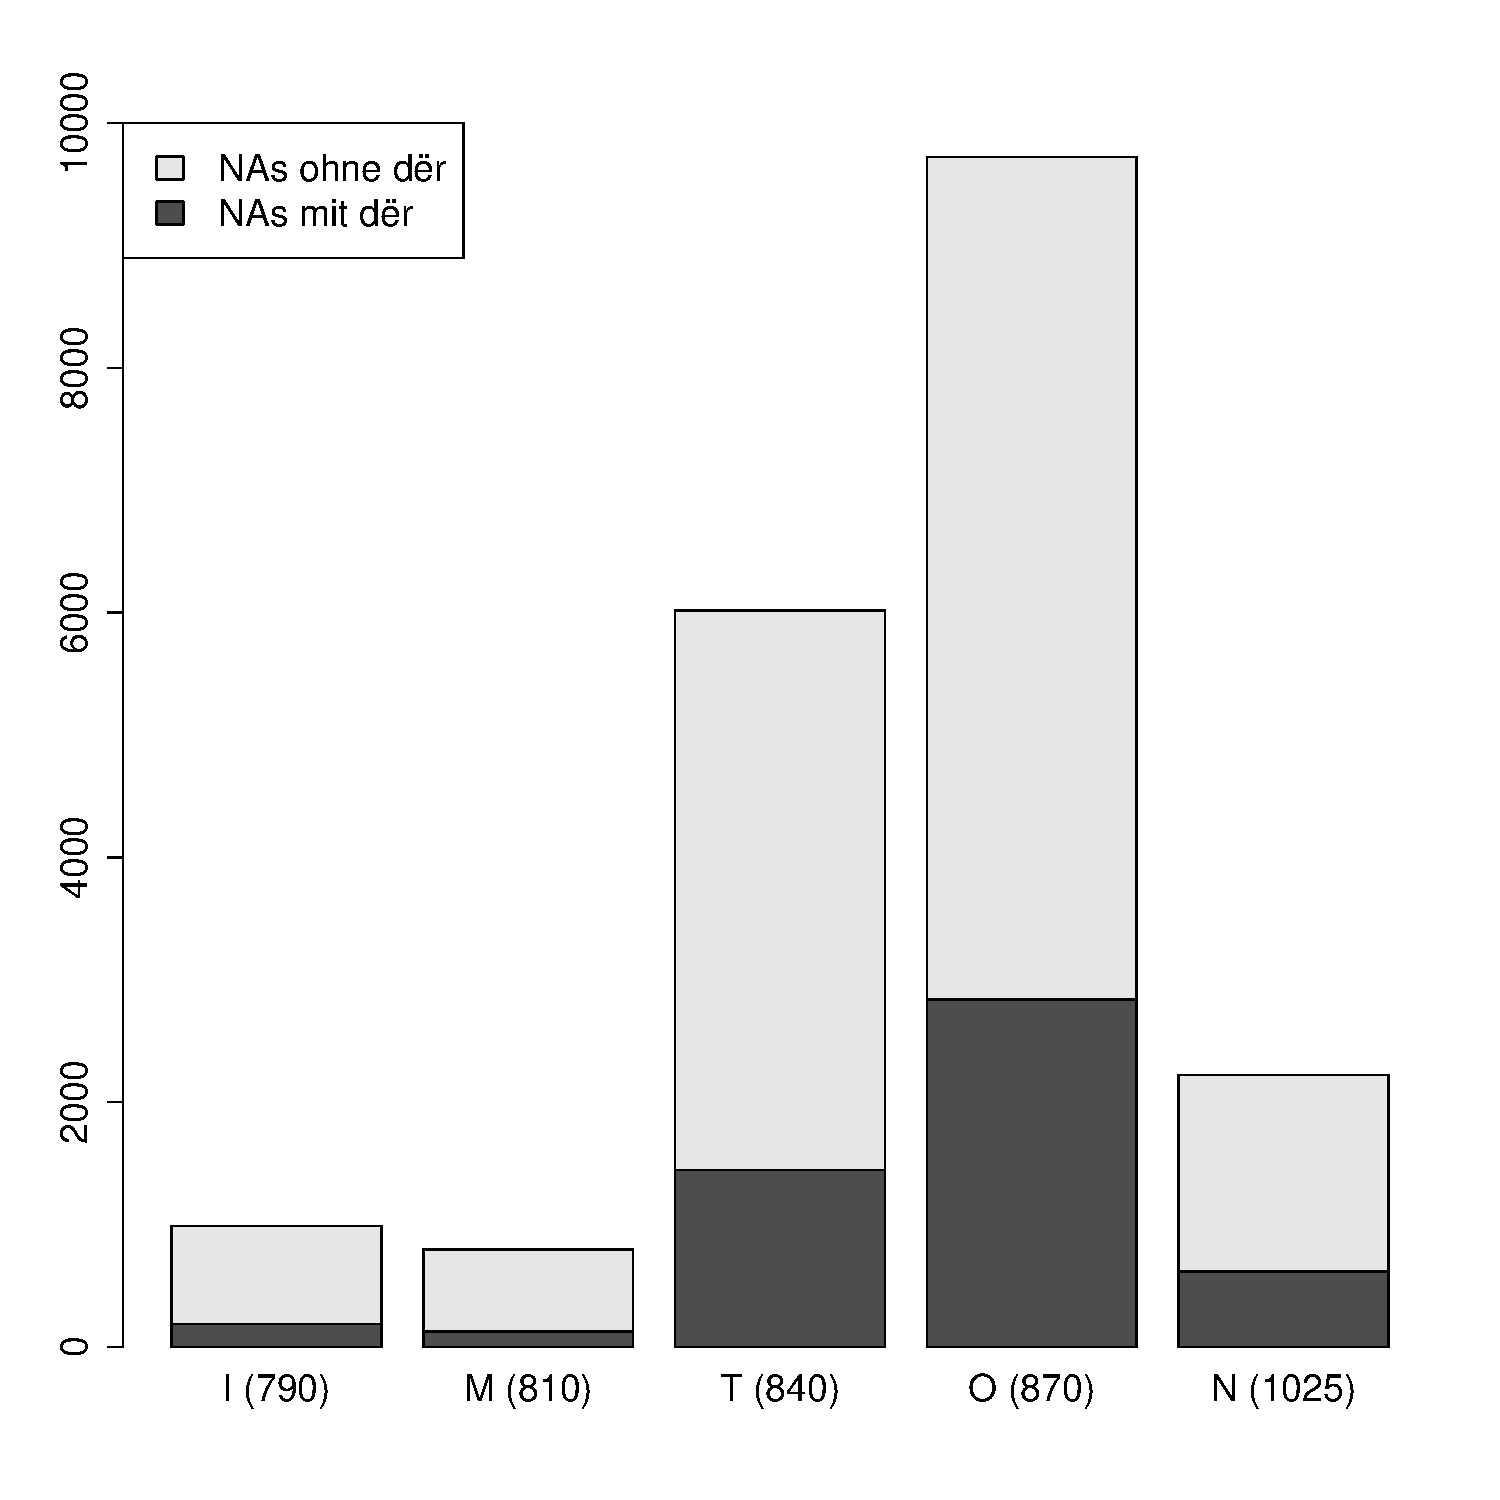
\includegraphics[width=\linewidth]{generated/images/artikel-anzahl-abs}
\caption {Absolute Zahlen}
\label{fig:art-abs}
\end{subfigure}%
\begin{subfigure}[b]{.5\linewidth}
  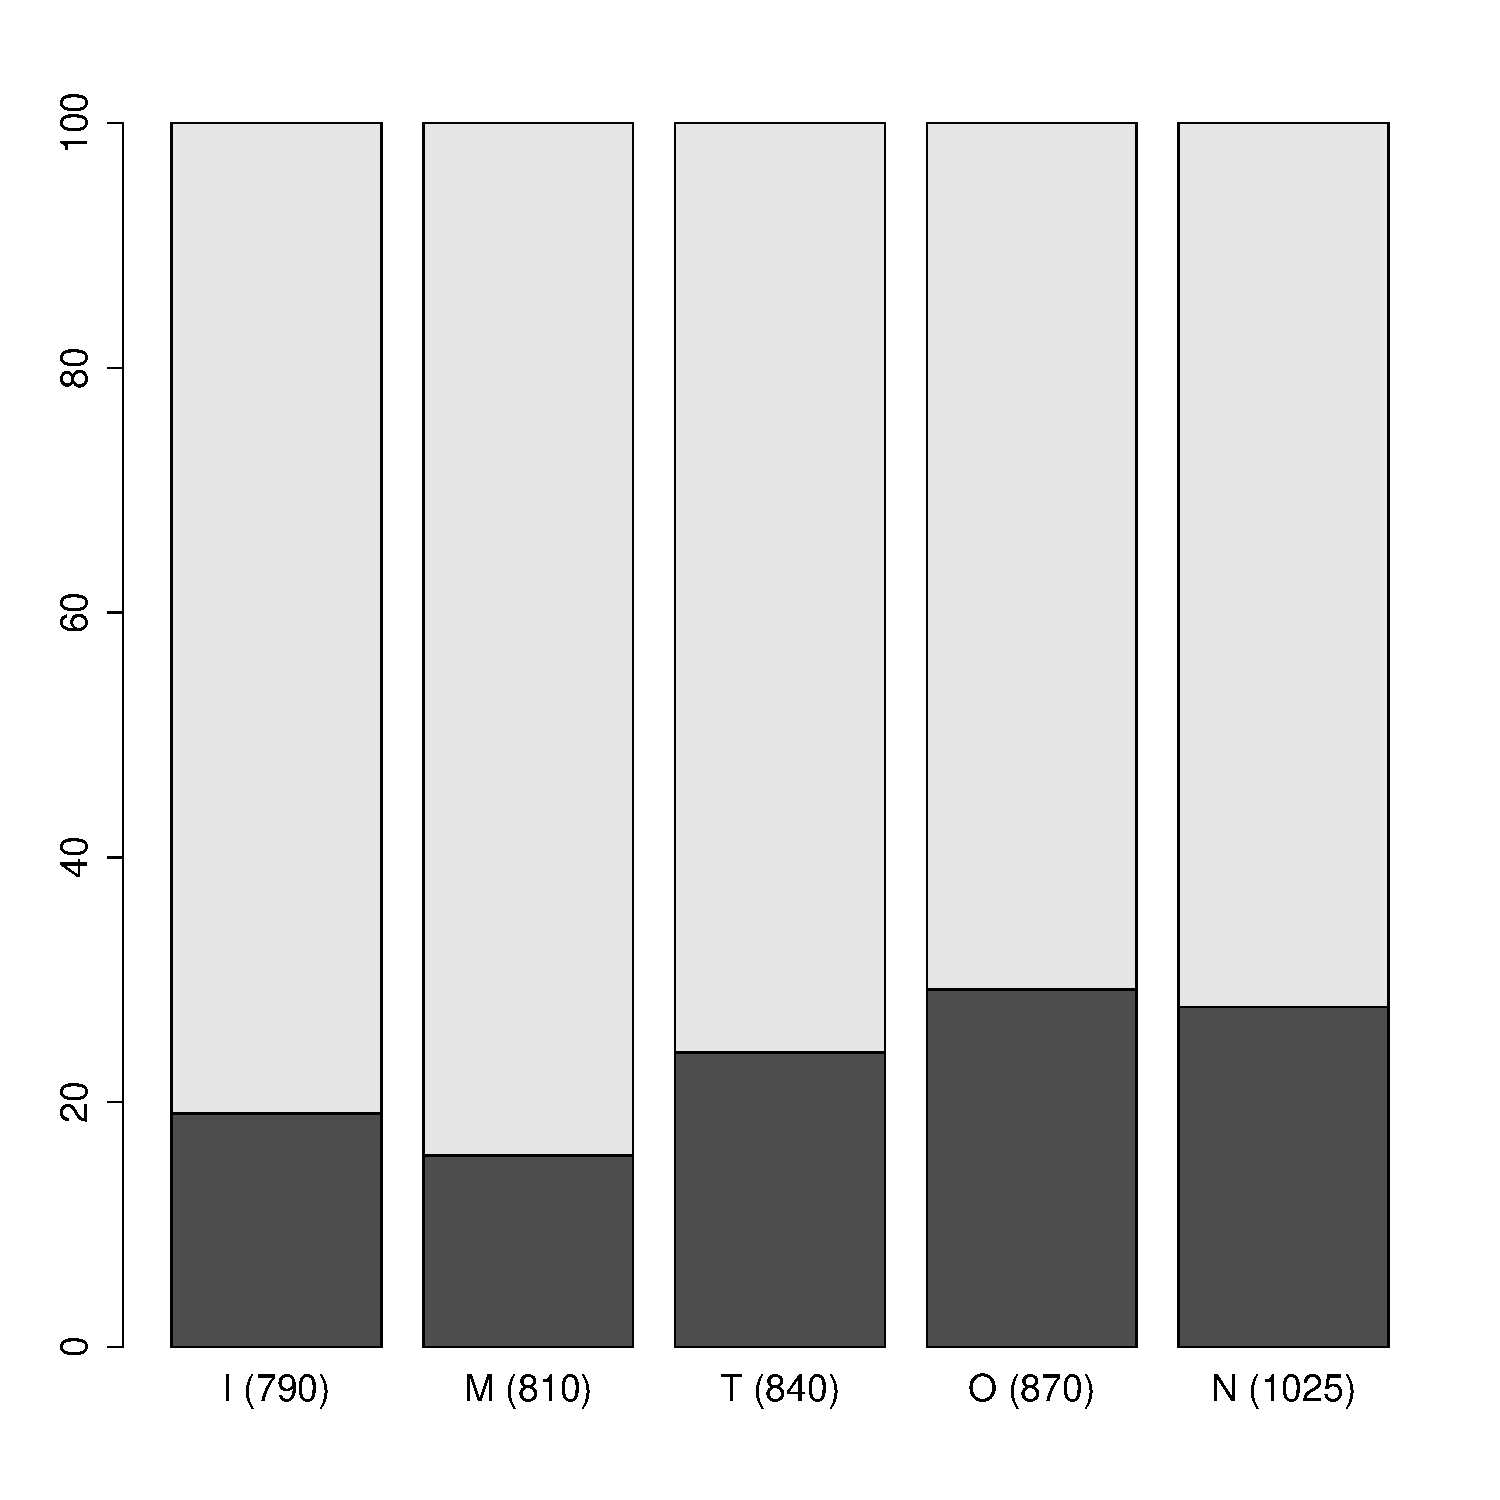
\includegraphics[width=\linewidth]{generated/images/artikel-anzahl-rel}
\caption {Relative Zahlen}
\label{fig:art-rel}
\end{subfigure}
\caption{Frequenz von \object{dër}}
\label{abb:art-freq}
\end{figure}
\vfill\pagebreak


Die relativen Zahlen auf der rechten Seite in Abbildung~\ref{abb:art-freq} verdeutlichen, dass \object{dër} immer mehr an Frequenz gewinnt.
Das älteste Denkmal (Isidor) sowie die jüngste Überlieferung (Notker) fallen allerdings aus der Reihe: Die Frequenzunterschiede zwischen Isidor und Monseer Matthäus sowie Otfrid und Notker sind jedoch nicht signifikant ($p > 0{,}05$, $\chi^2$-Test) und lassen sich vermutlich auf die Textsorte zurückführen. Wie schon in Abschnitt \ref{sec:textauswahl} erläutert, sind beim argumentativ ausgerichteten Isidor Bezüge auf zuvor genannte bzw. zentrale biblische Referenten häufig. Das Artikelwort \object{dër} kann helfen, diese Bezüge herzustellen. Doch wie die Ausführungen in \ref{sec:ergeb-defkontexte} zeigen werden, nutzt der Isidor-Übersetzer \object{dër} durchaus auch in semantischen Definitheitskontexten \is{Semantische Definita} und erweist sich dementsprechend als äußerst progressiv. Als einziger philosophischer Text enthält Notkers Boethius naturgemäß viele \is{Abstraktum} Abstrakta, die entsprechend lange undeterminiert bleiben und damit die \object{dër}-Frequenz nach unten drücken (vgl. hierzu Abschnitt \ref{sec:ergeb-faktoren}). 
Die Frequenzunterschiede zwischen den drei zeitlich dazwischen liegenden Schriftstücken sind hingegen hoch signifikant ($p < 0{,}001$, $\chi^2$-Test). Dabei sind der Monseer Matthäus, Tatian und Otfrid gut miteinander vergleichbar: Sie bestehen jeweils aus Erzählungen über die Taten Christi. Es scheint zudem, als würde auch das Reimschema \is{Reim} bei Otfrids Evangelienbuch (dem einzigen poetischen Text) dem Gebrauch von \object{dër} als Phraseneinleiter nicht entgegenstehen.  

\section{Das funktionale Spektrum von \object{dër}}\label{sec:ergeb-definitheit}

In Abschnitt \ref{sec:ergeb-defkontexte} werden die Ergebnisse der Stichprobenanalyse zu den Definitheitskontexten \is{Definitheitskontext} im Isidor, Tatian und bei Otfrid präsentiert. Anschließend fokussieren die Daten in Abschnitt \ref{sec:ergeb-superaltiv} und \ref{sec:ergeb-monosem} genuin abstrakt-definite Gebrauchskontexte, indem zunächst alle Superlativkonstruktionen \is{Superlativ} und dann ausgewählte Unika \is{Unikum} in den Texten betrachtet werden.  

\subsection{Definitheitskontexte}\label{sec:ergeb-defkontexte}

Pro Text wurde eine zufällige Stichprobe von 100 \isi{Token} mit dem PoS-Tag \hervor{NA} (Nomen Appellativum) \is{Gattungsname} ausgewählt und nach Definitheits- bzw. Indefinitheitskontexten \is{Indefinitheit}\is{Definitheitskontext}annotiert. Die nachfolgenden Werte entsprechen Nomen, die den Kern einer NP in Satzgliedfunktion bilden.\footnote{Die Stichprobe kann im R-Skript \hervor{aufbereitung.annotierte.daten} nachvollzogen werden. Dieses kann ebenso wie die annotierten Daten in \textcite{HZKYL4_2020} eingesehen werden.}   
Zentral für den funktionalen Wandel, ist die Frage, ob und in welchem Maße
[\object{dër}\,+\,N]-Phrasen \is{Phrase} gebraucht werden, um Referenten zu denotieren, die auch ohne explizite Vorerwähnung im Text oder im größeren Diskurskontext für den Adressaten identifizierbar sind, d.h. in den semantischen Definitheitskontexten \is{Semantische Definita} auftreten (vgl. Abschnitt \ref{sec:pragsem}). Ambige Fälle, die in allen Texten vorgekommen sind, werden später in Abschnitt \ref{sec:disk-bruecken} als mögliche Brückenkontexte \is{Brückenkontext} analysiert. 

%\subsubsection{Isidor} 

In der nachfolgenden Tabelle ist die Verteilung der 
100 annotierten NPs aus dem Isidor auf die unterschiedlichen Kontexttypen dargestellt. 16 der 100 NPs tragen ein \object{dër}.


\begin{table}
\centering
\begin{tabular}{llrrr}
\lsptoprule
{Definitheitsart}                                 & {Gebrauchskontexte}        & {mit \object{dër}} & {ohne \object{dër}} & {Summe} \\ \midrule
\multirow{4}{*}{Pragmatisch} & Situativ               & 0       & 0        & 0      \\
                                          & Anaphorisch            & 3       & 2        & 5      \\
                                          & Diskursdeiktisch       & 0       & 1        & 1      \\
                                          & Anamnestisch           & 2       & 0        & 2      \\ \midrule
\multirow{4}{*}{Semantisch}  & Abstrakt-situativ      & 7       & 25       & 32     \\
                                          & Assoziativ-anaphorisch & 0       & 1        & 1      \\
                                          & Monoreferenz                      & 1       & 17       & 18     \\
                                          & Generisch              & 1       & 6        & 7      \\ \midrule
\multirow{3}{*}{Nicht-definit}  & Nicht-spezifisch       & 0       & 11       & 11 \\
                                          & Spezifisch-indefinit   & 0       & 1        & 1      \\
                                          & Indefinit              & 0       & 6        & 6      \\ \midrule
\multirow{2}{*}{Andere Fälle}                   & mit Possessiva                    & 0       & 12       & 12     \\
                                          & Ambige Fälle                      & 2       & 2        & 4      \\ \midrule
\multicolumn{2}{c}{Summe}                                                    & 16      & 84       & 100    \\ \lspbottomrule
\end{tabular}
\caption{Definitheits- und Indefinitheitskontexte \is{Indefinitheit}\is{Definitheitskontext}im Isidor}
\label{tab:definitheit-I}
\end{table}
%basierend auf: Stichprobe.Definitheit.R
%\inputtable{generated/tables/definitheit-I}{Definitheitskontexte im Isidor}{tab:definitheit-I}

Erwartet wurde, dass in diesem frühen ahd. Text vor allem Referenten mit [\object{dër}\,+\,N]-Phrasen \is{Phrase} denotiert werden, die durch den unmittelbaren Text oder einen vorherigen Diskurs vorerwähnt sind und dadurch identifizierbar wurden \is{Pragmatische Definita} (=\,prag\-ma\-tische Gebrauchskontexte). Daher überrascht es, dass nur fünf der 16 Phrasen diesem Definitheitstypus entsprechen (3 $\times$ anaphorisch \is{anaphorisch} und 2 \is{anamnestisch} $\times$ anamnestisch). In Beispiel \REF{ex:I1051} ist ein Beleg für den  anaphorischen Gebrauch \is{anaphorisch} aufgeführt. Mit \object{dher aerlose man} wird auf einen  zuvor erwähnten König Bezug genommen.  

% Basis:
%\begin{exe}
\ex \label{ex:I1051} \gll \object{Ibu} \object{dhanne} \object{einic} \object{chilaubit} \object{0} \object{dhazs} \object{dhiz} \object{fona} \object{cyre} \object{persero} \object{chuninge} \object{sii} \object{chiforabodot} \object{0} \object{bichnaa} \object{sih} \object{dher} \object{0} \object{dhazs} \object{izs} \object{uuidharzuomi} \object{endi} \object{heidhanliih} \object{ist} \object{eomanne} \object{zi} \object{chilaubanne} \object{0} \object{dhazs} \object{dher} \object{aerloso} \object{\underline{man}} \object{endi} \object{dher} \object{heidheno} \object{abgudim} \object{gheldendo} \object{christ} \object{0} \object{got} \object{endi} \object{druhtin} \object{uurdi} \object{chinemnit} \object{. } \\
{wenn} {dann} {irgendein} {glauben} {} {dass} {dieser} {von} {Kyrus} {Perser} {König} {sein} {ankündigen} {} {klarmachen} {sich} {der} {} {dass} {er} {widersinnig} {und} {heidnisch} {sein} {(irgend)jemand} {zu} {glauben} {} {dass} {der} {gottlos} {Mann} {und} {der} {Heide} {Götzen(bilder)} {geben} {Christus} {} {Gott} {und} {Herr} {werden} {nennen} {}\\
\glt TODO: nhd. Übersetzung (I.3,3)
\end{exe}


\begin{exe}
\ex \label{ex:I1051} \gll  dhazs dhiz fona cyre persero chuninge dhazs \textit{dher} \textit{aerloso} \textit{man} \\
{dass} {dieser} {von} {Kyrus} {Perser} {König} {dass} {dieser} {gottlose} {Mann} \\
\glt   \extrans{dass dieser Perserkönig von Kyrus dass  dieser gottlose Mann} (I 3,3)
\end{exe}

Der Beleg in \REF{ex:I2524} ist exemplarisch für den anamnestischen \is{anamnestisch} Gebrauch. Für die \isi{Phrase} \object{dhurach dhen selbun heilegun forasagun} gibt es keinen unmittelbar vorerwähnten Antezedens. Trotzdem kann man davon ausgehen, dass die Leserschaft weiß, dass es sich um den Propheten handelt, der schon in einigen Abschnitten vorher erwähnt wurde.
%Basis
%\begin{exe}
\ex \label{ex:I2524} \gll \object{So} \object{auh} \object{in} \object{andreru} \object{stedi} \object{dhurah} \object{dhen} \object{selbun} \object{heilegun} \object{\underline{forasagun}} \object{uuard} \object{dhera} \object{dhrinissa} \object{bauhnunc} \object{sus} \object{araughit} \object{: } \\
{so} {auch} {in} {anderer} {Stätte} {durch} {der} {selber} {heilig} {Prophet} {werden} {der} {Dreiheit} {Bezeichnung} {so} {offenbaren} {}\\
\glt TODO: nhd. Übersetzung (I.4,8)
\end{exe}


\begin{exe}
\ex \label{ex:I2524} \gll So auh in andreru stedi \textit{dhurah} \textit{dhen} \textit{selbun} \textit{heilegun} \textit{forasagun} uuard dhera dhrinissa bauhnunc sus araughit  \\
{so} {auch} {in} {anderer} {Stelle} {durch} {den} {selben} {heiligen} {Propheten} {ward} {der} {Dreifaltigkeit} {Bezeichnung} {so} {offenbart} \\
\glt   \extrans{Auch an andere Stelle wird durch diesen selben heiligen Propheten die Bezeichnung der Dreifaltigkeit offenbart.} (I 4,8)
\end{exe}

Mit den restlichen [\object{dër}\,+\,N]-Belegen werden Referenten denotiert, die auch ohne den Kontext eindeutig identifizierbar sind. In einem Fall liegt Monoreferenz vor. Die \object{dër}-\isi{Phrase} ist in eine indirekte Frage eingebettet: \object{huueo dher sunu mahti fona fater chiboran uuerdhan} \extrans{wie der Sohn vom Vater (Gott) geboren werden konnte} (I 2,3). 

In \REF{ex:I683} ist ein Beispiel für den abstrakt-situativen \is{abstrakt-situativ} Gebrauch. 
%Basis
%\begin{exe}
\ex \label{ex:I683} \gll \object{Christus} \object{auur} \object{sus} \object{quham} \object{fona} \object{fater} \object{ziuuaare} \object{so selp so} \object{dhiu} \object{\underline{berahtnissi}} \object{fona} \object{sunnun} \object{0} \object{so} \object{uuort} \object{fona} \object{munde} \object{0} \object{so} \object{uuiisduom} \object{fona} \object{herzin} \object{. } \\
{Christus} {aber} {so} {kommen} {von} {Vater} {gewiss} {ebenso wie} {der} {Ehre} {von} {Sonne} {} {so} {Wort} {von} {Mund} {} {so} {Weisheit} {von} {Herz} {}\\
\glt TODO: nhd. Übersetzung (I.2,5)
\end{exe}

\begin{exe}
\ex \label{ex:I683} \gll {Christus} {auur} {sus} {quham} {fona} {fater} {ziuuaare} {so selp so} {\textit{dhiu}} {\textit{berahtnissi}} {fona} {sunnun}, {so} {uuort} {fona} {munde}, {so} {uuiisduom} {fona} {herzin} \\
{Christus} {aber} {so} {kam} {von} {Vater} {gewiss} {ebenso wie} {der} {Glanz} {von} {Sonne}, {so} {Wort} {von} {Mund}, {so} {Weisheit} {von} {Herz} {}\\
\glt \extrans{Christus aber kam gewiss vom Vater genauso wie der Glanz von der Sonne, wie das Wort vom Mund, die Weisheit vom Herz} (I 2,5)
\end{exe}

Interessanterweise konnte ein \object{dër}-Beleg auch als generisch \is{generisch} klassifiziert werden, s. \REF{ex:I4768}. Mit \object{dhea iudea} wird eine allgemeine Charakterisierung über die Juden vorgenommen. 
%Basis:
%\begin{exe}
\ex \label{ex:I4768} \gll \object{Dhea} \object{\underline{iudea}} \object{auur} \object{dhurah} \object{iro} \object{grimmin} \object{mit} \object{dhemu} \object{unscama} \object{habendin} \object{andine} \object{quhedhant} \object{leogando} \object{dhazs} \object{noh} \object{ni} \object{sii} \object{dhazs} \object{ziidh} \object{arfullit} \object{0} \object{ni} \object{uueizs} \object{ih} \object{einigan} \object{chuninc} \object{fona} \object{iudases} \object{edhile} \object{noh} \object{in} \object{uzssonondem} \object{endum} \object{oostarriihhes} \object{uualdendan} \object{. } \\
{der} {Juden} {aber} {durch} {er} {Grimm} {mit} {der} {Schamlosigkeit} {haben} {Stirn} {sprechen} {lügen} {dass} {noch} {nicht} {sein} {der} {Zeit} {erfüllen} {} {nicht} {wissen} {ich} {irgendein} {König} {von} {Judas} {Adel} {noch} {in} {äußerst} {Ende} {Ost(franken)reich} {walten} {}\\
\glt TODO: nhd. Übersetzung (I.8,2)
\end{exe}


\begin{exe}
\ex \label{ex:I4768} \gll {\textit{Dhea}} {\textit{iudea}} {auur} {dhurah} {iro} {grimmin} {mit} {der} {unscama} {habendin} {andine} {quhedhant} {leogando} {dhazs}\\
{der} {Juden} {aber} {durch} {ihren} {Ingrimm} {mit} {der} {Schamlosigkeit} {haben} {Stirn} {sprechen} {lügend} {dass}\\
\glt \extrans{Aber die Juden sagen durch ihren Ingrimm mit Schamlosigkeit lügend, dass}(I 8,2)
\end{exe}

In allen 16 Fällen erfolgt die \object{dër}-Setzung entgegen der Vorlage, so dass lateinischen Interferenzen ausgeschlossen werden können. Zu den nicht-spezifischen Referenten \is{Spezifizität} gehören adverbiale \is{Adverbial} Angaben wie \object{duruh riuwa} \extrans{durch Reue}(I 5,10) oder Nomen in Funktionsverbefügen wie \object{man wërdan} \extrans{Mensch werden} (I 5,1). Der eine spezifisch-indefinite \is{Spezifizität} Beleg bezieht sich auf die \isi{Phrase} \object{mit sumes chirunes uuagu} \extrans{mit einer gewissen Waage} (I 4,9). In der Gruppe \hervor{indefinite Referenten} addieren sich Belege mit weniger salienten und unspezifischen \is{Spezifizität} Referenten wie \object{oba drato
hoh hohsedal} \extrans{auf einem hohen Thron} (I 4,10). Die Gruppe \hervor{mit Possessiva} \is{Possessivum}enthält \is{Phrase} Phrasen, die durch einen \is{Possessivum} Possessivartikel eingeleitet werden. 

%\subsubsection{Tatian} 

Im Vergleich zum Isidor nehmen im Tatian die semantisch-definiten Kontexte \is{Semantische Definita} mehr Raum ein. Wie in Tabelle~\ref{tab:definitheit-T} zu sehen ist, enthalten knapp ein Drittel (11 von 35 Belege) der abstrakt-situativen \is{abstrakt-situativ} Gebrauchskontexte ein \object{dër}.

\begin{table}
\centering
\begin{tabular}{llrrr}
\lsptoprule
{Definitheitsart}                                 & {Gebrauchskontext}        & {mit \object{dër}} & {ohne \object{dër}} & {Summe} \\ \midrule
\multirow{4}{*}{Pragmatisch} & Situativ               & 0       & 1        & 1      \\
                                          & Anaphorisch            & 1       & 3        & 4      \\
                                          & Diskursdeiktisch       & 0       & 1        & 1      \\
                                          & Anamnestisch           & 1       & 0        & 1      \\ \midrule
\multirow{4}{*}{Semantisch}  & Abstrakt-situativ      & 11       & 24       & 35 \\
                                          & Assoziativ-anaphorisch & 2       & 1        & 3      \\
                                          & Monoreferenz                      & 10       & 1       & 11     \\
                                          & Generisch              & 0       & 4        & 4      \\ \midrule
\multirow{3}{*}{Nicht-definit}  & Nicht-spezifisch       & 0       & 10       & 10     \\
                                          & Spezifisch-indefinit   & 0       & 2        & 2      \\
                                          & Indefinit              & 0       & 9        & 9      \\ \midrule
\multirow{2}{*}{Andere Fälle}                   & mit Possessiva                    & 0       & 14       & 14     \\
                                          & Ambige Fälle                      & 2       & 3        & 5      \\ \midrule
\multicolumn{2}{c}{Summe}                                                    & 27      & 73       & 100    \\ \lspbottomrule
\end{tabular}
\caption{Definitheits- und Indefinitheitskontexte \is{Indefinitheit}\is{Definitheitskontext}im Tatian}
\label{tab:definitheit-T}
\end{table}

%%basierend auf:
%\inputtable{generated/tables/definitheit-T}{Definitheitskontexte im Tatian}{tab:definitheit-T}

 Die Fälle von Monoreferenz mit \object{dër} beziehen sich immer auf \object{Jesus}; 8 Mal steht es in Kombination mit \object{heilant}, ansonsten mit \object{sun}. Zudem finden sich unter den insgesamt 27 \object{dër}-Phrasen \is{Phrase} auch zwei assoziativ-anaphorische \is{assoziativ-anaphorisch} Kontexte, s. hierfür exemplarisch der Beleg in \REF{ex:T27561}. 

% Basis 
%\begin{exe}
\ex \label{ex:T27561} \gll \object{Maria} \object{habenti} \object{salbfaz} \object{salbun} \object{fon} \object{narthu} \object{gitana} \object{diura} \object{0} \object{inti} \object{gibrohanemo} \object{goz} \object{ubar} \object{sin} \object{houbit} \object{linentes} \object{0} \object{inti} \object{salbota} \object{sine} \object{fuozi} \object{inti} \object{suarb} \object{mit} \object{ira} \object{locon} \object{0} \object{inti} \object{thaz} \object{hus} \object{uuas} \object{gifullit} \object{fon} \object{themo} \object{\underline{stanke}} \object{thera} \object{salbun} \object{.} \\
{Maria} {haben} {Salbgefäß} {Salbe} {von} {Narde(nöl)} {tun} {teuer} {} {und} {(ab)brechen} {(ver)gießen} {über} {sein} {Haupt} {niedersinken} {} {und} {(ein)salben} {sein (eigen)} {Fuß} {und} {abreiben} {mit} {er} {Locke} {} {und} {dieser} {Haus} {sein} {(er)füllen} {von} {dieser} {(Wohl)geruch} {dieser} {Salbe} {}\\
\glt TODO: nhd. Übersetzung (T.138,1)
\end{exe}


\begin{exe}
\ex \label{ex:T27561} \gll {inti} {salbota} {sine} {fuozi} {inti} {suarb} {mit} {ira} {locon}, {inti} {thaz} {hus} {uuas} {gifullit} {fon} {\textit{themo}} {\textit{stanke}} {thera} {salbun}  \\
{und} {salbte} {seinen } {Fuß} {und} {rieb} {mit} {ihren} {Locken}, {und} {das} {Haus} {war} {erfüllt} {von} {dem} {Geruch} {der} {Salbe} \\
\glt \extrans{Und sie salbte seine Füße und trocknete sie mit ihren Haaren ab und das Haus war mit dem Geruch der Salbe gefüllt} (T 138,1)
\end{exe}

Generische Phrasen mit \object{dër} waren in der Stichprobe nicht dabei. Die Untersuchung von \textcite{Oubouzar1989,Oubouzar1992} hat allerdings gezeigt, dass diese im Tatian durchaus vorhanden sind (vgl. auch Abschnitt \ref{sec:pragsem}). Alle \object{dër}-Setzungen sind \is{Differenzbeleg} Differenzbelege, d.h. in der lateinischen Vorlage gibt es keine \isi{Demonstrativartikel} als Äquivalent.

%\subsubsection{Otfrid} 

Tabelle~\ref{tab:definitheit-O} zeigt die Verteilung der definiten bzw. indefiniten Gebrauchskontexte auf die 100 NPs bei Otfrid. Fast die Hälfte aller abstrakt-situativen \is{abstrakt-situativ} Gebrauchskontexte (18 von 37 Belege) werden hier mithilfe von \object{dër}-Phrasen \is{Phrase} zum Ausdruck gebracht.

\begin{table}
\centering
\begin{tabular}{llrrr}
\lsptoprule
{Definitheitsart}                                 & {Gebrauchskontext}        & {mit \object{dër}} & {ohne \object{dër}} & {Summe} \\ \midrule
\multirow{4}{*}{Pragmatisch} & Situativ               & 0                & 1                 & 1 \\
                                          & Anaphorisch            & 1                & 1 & 2               \\
                                          & Diskursdeiktisch       & 0                & 1                 & 1               \\
                                          & Anamnestisch           & 0                & 0                 & 0               \\  \midrule
\multirow{4}{*}{Semantisch}  & Abstrakt-situativ      & 18                & 19 & 37              \\
                                          & Assoziativ-anaphorisch & 0                & 0                 & 0               \\
                                          & Monoreferenz                      & 0                & 5                & 5              \\
                                          & Generisch              & 2                & 2                 & 4               \\  \midrule
\multirow{3}{*}{Nicht-definit}  & Nicht-spezifisch       & 0                & 22                & 22              \\
                                          & Spezifisch-indefinit   & 0                & 1                 & 1               \\
                                          & Indefinit              & 0                & 11                 & 11               \\  \midrule
\multirow{2}{*}{Andere Fälle}                   & mit Possessiva                    & 1                & 11                & 12              \\
                                          & Ambige Fälle                      & 2                & 2                 & 4               \\  \midrule
\multicolumn{2}{c}{Summe}                                                    & 24               & 76                & 100             \\ \lspbottomrule
\end{tabular}
\caption{Definitheits- und Indefinitheitskontexte \is{Indefinitheit}\is{Definitheitskontext}bei Otfrid}
\label{tab:definitheit-O}
\end{table}\pagebreak

% basierend auf\inputtable{generated/tables/definitheit-O}{Definitheitskontexte im Otfrid}{tab:definitheit-O}

Fälle von assoziativ-anaphorischer \is{assoziativ-anaphorisch} Definitheit sind in der Stichprobe nicht belegt. Generische Ausdrücke kommen gleich häufig mit (vgl. \ref{ex:O62652}) und ohne (vgl. \ref{ex:O72468}) \object{dër} vor.

% Basis:
%\begin{exe}
\ex \label{ex:O62652} \gll \object{Ther} \object{\underline{mán}} \object{ther} \object{thaz} \object{súachit} \object{thes} \object{er} \object{hárto} \object{ruachit} \object{:} \\
{der} {Mensch; Mann} {der} {der} {suchen} {der} {er} {sehr} {sich sehnen} {}\\
\glt TODO: nhd. Übersetzung (O.5,7)
\end{exe}


\begin{exe}
\ex \label{ex:O62652} \gll {\textit{Ther}} {\textit{mán}} {ther} {thaz} {súachit} {thes} {er} {hárto} {ruachit} \\
{der} {Mensch} {der} {das} {sucht} {dessen} {er} {sehr} {sich sehnt} \\
\glt   \extrans{Der Mensch, der das sucht, wonach er sich sehr sehnt} (O V,7)
% Basis
%\begin{exe}
\ex \label{ex:O72468} \gll \object{Hiar} \object{síudit} \object{\underline{mánne}} \object{ana} \object{wánk} \object{io} \object{ther} \object{úbilo} \object{githánk} \object{in} \object{hérzen} \object{joh} \object{in} \object{múate} \object{0} \object{ni} \object{firséhent} \object{sih} \object{zi} \object{gúate} \object{;} \\
{hier} {brennen} {Mensch; Mann} {ohne} {Zweifel} {immer} {der} {übel} {Gedanke; Gesinnung} {in} {Herz} {und} {in} {Sinn} {} {nicht} {schauen} {sich} {zu } {Gutes} {}\\
\glt TODO: nhd. Übersetzung (O.5,23)
\end{exe}


\ex \label{ex:O72468} \gll {Hiar} {síudit} {\textit{mánne}} {ana} {wánk} {io} {ther} {úbilo} {githánk} {in} {hérzen} {joh} {in} {múate}  \\
{hier} {brennt} {(dem) Menschen} {ohne} {Zweifel} {immer} {der} {übel} {Gedanke} {in} {Herz} {und} {in} {Gemüt} \\
\glt   \extrans{Hier brennt dem Menschen zweifellos der üble Gedanke im Herzen und im Gemüt}  (O V,23)
\end{exe}

Die Anzahl der \object{dër}-Phrasen \is{Phrase} im Bereich der semantischen Definita \is{Semantische Definita} ist bei Otfrid im Vergleich zu den beiden älteren Texten also größer. In den pragmatischen Definitheitskontexte \is{Pragmatische Definita} findet sich hingegen nur ein Beleg mit \object{dër}, und zwar im Rahmen eines anaphorischen \is{anaphorisch} Kontexts. Der eine Beleg für den diskursdeiktischen \is{diskursdeiktisch} Bezug wird mit \object{dëser} \is{Demonstrativum}eingeleitet (\object{in thésera noti} \extrans{in dieser Not(lage))}; O III 20), ebenso wie der Beleg mit situativer Referenz \is{situativ} \object{these kísila} \extrans{dieser Kieselstein} (O I,23) sowie der zweite anaphorische \is{anaphorisch} Beleg. Die Ergebnisse sprechen dafür, dass sich [\object{dër}\,+\,N] als Ausdruck für semantische Definitheitskontexte \is{Semantische Definita} etabliert hat. Die Setzung ist allerdings nicht obligatorisch. Die Struktur [\object{dëser}\,+\,N] scheint sich hingegen auf pragmatische Definita \is{Pragmatische Definita} spezialisiert zu haben; bei den semantischen Definita \is{Semantische Definita} kommt sie nicht vor.

\subsection{Superlative}\label{sec:ergeb-superaltiv}

Superlative \is{Superlativ} sind Indikatoren für semantisch-definite \is{Semantische Definita} Gebrauchskontexte  (vgl.\linebreak Abschnitt \ref{sec:nicht-fam}), da unabhängig von der Äußerungssituation  immer nur ein Referent in Frage kommt, der als \object{die beste Schauspielerin} oder \object{das Schönste} ausgezeichnet werden kann. Sprachen mit \isi{Definitartikel} setzen in diesen Kontexten immer einen \isi{Definitartikel} \parencite{Himmelmann2001}. Der Austausch mit einem \isi{Demonstrativum} ist hier nicht möglich. Denn es geht bei dieser Artikelsetzung nicht darum, einen bestimmten Referenten (in Abgrenzung zu anderen potentiellen Referenten) identifizierbar zu \hervor{machen}, sondern die definite Lesart lediglich als solche zu markieren \parencite[41]{Himmelmann1997}.

In Tabelle~\ref{tab:superlative} werden die Häufigkeiten der attributiven Adjektive \is{Adjektiv} im \isi{Superlativ} mit und ohne \object{dër} miteinander verglichen. Tabelle~\ref{tab:subst:superlative} zeigt, wie viele substantivierte \is{Substantivierung} Superlative \is{Superlativ} mit \object{dër} determiniert werden. In beiden Fällen wurde ein Beleg genau dann als mit \object{dër} determiniert gezählt, wenn dem \isi{Superlativ} ein \isi{Token} mit dem PoS-Tag \hervor{DDA} unmittelbar vorausgeht und mit diesen in \isi{Kasus}, \isi{Genus} und \isi{Numerus} übereinstimmt. 

Man sieht, dass der Strukturtyp \is{Superlativ}\is{Adjektiv}[\object{dër}\,+\,Adjektiv\textsubscript{Superlativ}\,+\,N] in allen Texten deutlich häufiger vorkommt als der Strukturtyp [Adjektiv\textsubscript{Superlativ}\,+\,N]. Bei den substantivierten Adjektiven \is{Substantivierung}\is{Adjektiv}gibt es hingegen nur im Tatian und bei Notker mehr Belege mit \object{dër} als ohne. Die wichtigste Beobachtung aus den Daten in Tabelle~\ref{tab:subst:superlative} ist, dass in allen Texten die Struktur \object{dër}\,+\,substantivierter \is{Substantivierung} \isi{Superlativ} belegt und damit grundsätzlich auch schon im frühen Althochdeutschen möglich ist. 

%basierend auf "Adjektive.R"
%\object{dër}-Setzung bei Superlativen: [(\object{dër}\,+\,) Ad\-jek\-tiv\textsubscript{Superlativ}\,+\,N)]
 
 
\begin{table}
\begin{tabular}{lrr}
\lsptoprule
              {Text}         & {mit \object{dër}} & {ohne \object{dër}} \\ \midrule
Isidor (790)           & 2                              & 0                           \\
Monseer Matthäus (810) & 4                              & 1                           \\
Tatian (840)           & 20                             & 7 \\
Otfrid (870)           & 7                            & 5                          \\
Notker (1025)          & 9                             & 1                           \\ \lspbottomrule
\end{tabular}
\caption{Strukturtypen im Vergleich: [\object{dër}\,+ Ad\-jek\-tiv\textsubscript{Superlativ}\,+\,N] vs. [Ad\-jek\-tiv\textsubscript{Superlativ}\,+\,N]}
\label{tab:superlative}
\end{table}

\begin{table}
\begin{tabular}{lrr}
\lsptoprule
              {Text}         & {mit \object{dër}} & {ohne \object{dër}} \\ \midrule
Isidor (790)           & 4                              & 6                           \\
Monseer Matthäus (810) & 3                              & 8                           \\
Tatian (840)           & 26                             & 13 \\
Otfrid (870)           & 2                            & 16                          \\
Notker (1025)          & 15                             & 3                           \\ \lspbottomrule
\end{tabular}
\caption{\object{dër}-Setzung bei substantivierten Superlativen}
\label{tab:subst:superlative}
\end{table}

\subsection{Unika} \label{sec:ergeb-monosem}

Unika \is{Unikum} referieren genau auf einen, im Diskursuniversum bekannten Referenten. Der Gebrauch eines demonstrativen \is{Demonstrativartikel} Artikelwortes, das der Referenzfindung bzw. -abgrenzung \is{Referentialität} dient, ist bei diesen Substantivtypen \is{Substantiv} überflüssig. Tritt ein \object{dër} bei Unika \is{Unikum} auf, ist dies daher ein gutes Indiz dafür, dass der funktionale Wandel Richtung \isi{Definitartikel} im Vollzug ist und das Muster [\object{dër}\,+\,N] sich auch auf semantisch-definite Kontexte \is{Semantische Definita} ausbreitet. Auf Basis der Studien von  \textcite{Graf1905}, \textcite{Bell1907}, \textcite{Hodler1954}, \textcite{Oubouzar1989} sowie der Fallstudie von \textcite[75]{Szczepaniak2011a} wurden Lemmata \is{Lemma} ausgewählt, die auf einzigartige und der ahd. Leserschaft bekannte Referenten verweisen: 

\begin{itemize}
\item Einmalige Referenten in der Natur\\
\object{sunna} \extrans{Sonne}, \object{mano} \extrans{Mond}, \object{himil} \extrans{Himmel}, \object{ërda} \extrans{Erde}, \object{wëralt} \extrans{Welt}
\item Unika aus dem christlichen Kulturkreis:\\
\object{heilant} \extrans{Jesus}, \object{geist} \extrans{(der heilige) Geist}, \object{got} \extrans{Gott},  \object{tiufal} \extrans{Teufel}
\end{itemize}

\noindent 
Die nachfolgenden Tabellen dokumentieren, ob \isi{Token} dieser Lemmata \is{Lemma} mit einem kongruierenden \object{dër} auftreten. Genau wie in Abschnitt \ref{sec:ergeb-ther-freq}  wurde hierfür für die Suche das gesamte \isi{Korpus} als Grundlage genommen und sowohl Fälle mit unmittelbarer Determination (\object{dër}\,+\,N) als auch Belege mit Distanzstellung (\object{dër}\,+\,X\,+\,N) einbezogen.
% Tabellen auf Basis von "lemma.R" 

Bei \object{sunna} und \object{mano} zeigt sich, dass in den frühen Schriftstücken keine Determination mit \object{dër} stattfindet, s. Tabellen~\ref{tab:sonne} und \ref{tab:mond}. 

\begin{table}
\begin{tabular}{lrr}
\lsptoprule
{Text}  & {mit \object{dër}} & {ohne \object{dër}} \\ \midrule
Isidor (790)           & 0                & 2                   \\
Monseer Matthäus (810) & 0                & 3                   \\
Tatian (840)           & 1                & 3                   \\
Otfrid (870)           & 4                & 15                  \\
Notker (1025)          & 10               & 7                   \\ \lspbottomrule
\end{tabular}
\caption{\object{dër}-Setzung bei \object{sunna} \extrans{Sonne}}
\label{tab:sonne}
\end{table}

\begin{table}
\begin{tabular}{lrr}
\lsptoprule
{Text}  & {mit \object{dër}} & {ohne \object{dër}}  \\ \midrule
Isidor (790)           & 0           & 1              \\
Monseer Matthäus (810) & 0           & 1              \\
Tatian (840)           & 0           & 2              \\
Otfrid (870)           & 1           & 3              \\
Notker (1025)          & 3           & 0              \\ \lspbottomrule
\end{tabular}
\caption{\object{dër}-Setzung bei \object{mano} \extrans{Mond}}
\label{tab:mond}
\end{table}

Im Tatian gibt es bei \object{sunna} genau einen Beleg mit \object{dër}, s. \REF{ex:T6760}. Interessanterweise steht, wie auch \textcite[20]{Graf1905} beobachtet, in der lateinischen Vorlage ein \isi{Possessivum}: \object{quia solem suum oriri facit}. Dies könnte laut \textcite[216]{Oubouzar1989} ein Beleg für die funktionale Überschneidung von \object{dër} mit determinierenden \is{Determinierer}\is{Possessivum}Possessiva sein.

%Basiert auf: 
%\begin{exe}
\ex \label{ex:T6760} \gll \object{Thaz} \object{ír} \object{sít} \object{kind} \object{íuuares} \object{fater} \object{thie} \object{in} \object{himile} \object{ist} \object{0} \object{ther} \object{thie} \object{\underline{sunnun}} \object{úf} \object{gangen} \object{tuot} \object{ubar} \object{ubile} \object{inti} \object{ubar} \object{guote} \object{inti} \object{reganot} \object{ubar} \object{rehte} \object{inti} \object{ubar} \object{únrehte} \object{.} \\
{daß} {ihr} {sein} {Kind} {euer} {Vater} {der} {in} {Himmel} {sein} {} {der} {der} {Sonne} {auf} {aufgehen} {tun} {über} {Übel} {und} {über} {Gute} {und} {regnen} {über} {Recht} {und} {über} {Unrecht} {}\\
\glt TODO: nhd. Übersetzung (T.32,3)
\end{exe}


\begin{exe}
\ex \label{ex:T6760} \gll {ther} {\textit{thie}} {\textit{sunnun}} {úf} {gangen} {tuot} \\
{der} {die} {Sonne} {auf} {gehen} {tut}  \\
\glt   \extrans{[Gott] der die Sonne aufgehen lässt} (T 32,3)
\end{exe}

Der erste Nachweis von \object{dër}\,+\,\object{mano} findet sich in Otfrids Evangelienbuch und zwar in einer Paarformel in Verbindung mit \object{sunna}, s. \REF{ex:O68453}.
%  basiert auf: 
%\begin{exe}
\ex \label{ex:O68453} \gll \object{Thia} \object{súnnun} \object{joh} \object{then} \object{\underline{mánon}} \object{so} \object{úbar} \object{fuar} \object{er} \object{gáhon} \object{0} \object{joh} \object{állan} \object{thesan} \object{wóroltring} \object{0} \object{ni} \object{gisah} \object{man} \object{ér} \object{io} \object{sulih} \object{thíng} \object{;} \\
{der} {Sonne} {und} {der} {Mond} {so} {über} {hinweggehen (über)} {er} {schnell} {} {und} {all} {dieser} {Erdkreis} {} {nicht} {sehen} {Mensch; Mann} {eher} {jemals} {solch} {Ding} {}\\
\glt TODO: nhd. Übersetzung (O.5,17)
\end{exe}

\begin{exe}
\ex \label{ex:O68453} \gll {\textit{Thia}} {\textit{súnnun}} {joh} {\textit{then}} {\textit{mánon}} {so} {úbar} {fuar} {er} {gáhon}  \\
{die} {Sonne} {und} {den} {Mond} {so} {über} {fährt} {er} {schnell} \\
\glt   \extrans{So überschreitet er die Sonne und den Mond schnell} (O V,17)
\end{exe}
\noindent 
Hier könnte die Setzung von \object{dër} auch metrisch \is{Metrik} bedingt sein \parencite[20]{Graf1905}. Dennoch kann man davon ausgehen, dass alleine die Möglichkeit, ein \object{dër} mit \object{mano} zu kombinieren, eine Abschwächung der demonstrativen Funktion voraussetzt. Erst bei Notker überwiegen sowohl bei \object{sunna} als auch bei \object{mano} die determinierten Belege, was auf eine  Koventionalisierung von [\object{dër}\,+\,N] hindeutet. Zur Illustration ist nachfolgend ein Beispiel aufgeführt, das sowohl [\object{dër}\,+\,\object{mano}] als auch [\object{dër}\,+\,\object{sunna}] enthält. 
%basiert auf:
%\begin{exe}
\ex \label{ex:N8884} \gll \object{dáz_} \object{ter} \object{mâno} \object{uuîlon} \object{fóllêr} \object{gâendo} \object{gágen} \object{dero} \object{\underline{súnnûn}} \object{. } \\
{dass} {der} {Mond} {bisweilen} {voll} {gehen} {gegen} {der} {Sonne} {}\\
\glt TODO: nhd. Übersetzung (N.1,31)
\end{exe}


\begin{exe}
\ex \label{ex:N8884} \gll {dáz} {\textit{ter}} {\textit{mâno}} {uuîlon} {fóllêr} {gâendo} {gágen} {\textit{dero}} {\textit{súnnûn}}  \\
{dass} {der} {Mond} {bisweilen} {voller} {gehend} {gegen} {der} {Sonne}\\
\glt   \extrans{dass der Mond bisweilen voller wird gegenüber der Sonne} (N 1,31)
\end{exe}

Ein ähnliches Bild zeigt sich auch für die Unika \is{Unikum} \object{himil},  \object{ërda} und \object{wëralt}, s. Tabellen~\ref{tab:himmel} bis~\ref{tab:welt}.     

\begin{table}[H]
\centering
\begin{tabular}{lrr}
\lsptoprule
{Text}  & {mit \object{dër}} & {ohne \object{dër}}  \\ \midrule
Isidor (790)           & 0                 & 1              \\
Monseer Matthäus (810) & 0                 & 1              \\
Tatian (840)           & 0                 & 2              \\
Otfrid (870)           & 6                 & 3              \\
Notker (1025)          & 15                & 0              \\ \lspbottomrule
\end{tabular}
\caption{\object{dër}-Setzung bei \object{himil} \extrans{Himmel}}
\label{tab:himmel}
\end{table}

\begin{table}[H]
\centering
\begin{tabular}{lrr}
\lsptoprule
{Text}  & {mit \object{dër}} & {ohne \object{dër}}  \\ \midrule
Isidor (790)           & 0  & 8     \\
Monseer Matthäus (810) & 0  & 12    \\
Tatian (840)           & 5  & 52    \\
Otfrid (870)           & 5  & 32    \\
Notker (1025)          & 12 & 9     \\ \lspbottomrule
\end{tabular}
\caption{\object{dër}-Setzung bei \object{ërda} \extrans{Erde}}
\label{tab:erde}
\end{table}\largerpage[2]

\begin{table}[H]
\centering
\begin{tabular}{lrr}
\lsptoprule
{Text}  & {mit \object{dër}} & {ohne \object{dër}}  \\ \midrule
Isidor (790)            & 1    & 2    \\
Monseer Matthäus (810) & 0     & 5    \\
Tatian (840)            & 4    & 43   \\
Otfrid (870)             & 15  & 140  \\
Notker (1025)           & 7    & 5    \\ \lspbottomrule
\end{tabular}
\caption{\object{dër}-Setzung bei \object{wëralt} \extrans{Welt}}
\label{tab:welt}
\end{table}

Obwohl \object{himil} in allen Texten immerhin mit  zweistelligen Tokenwerten vertreten ist, findet man in den drei ältesten Texten keinen Beleg in Kombination mit \object{dër}. Erst bei Otfrid treten die ersten Fälle auf. Bei \object{ërda} und \object{wëralt} sind bereits im Tatian schon determinierte Phrasen zu verzeichnen. Die Suchsyntax hat auch einen Beleg von \object{dër} + \object{wëralt} im Isidor hervorgebracht und zwar innerhalb eines \is{Genitivattribut} adnominalen Genitivs: \object{fater dhera zuohaldun uueraldi} (I 5,6). Die Setzung erfolgt sogar entgegen der Vorlage (lat. \object{pater futuri saeculi}). Möglicherweise löst das schwach flektierte \is{Flexion} \isi{Adjektiv} die \object{dër}-Setzung aus (s. Abschnitt \ref{sec:ergeb-adjflex}).
% hier ist der gesamte Beleg:
%\begin{exe}
\ex \label{ex:I3050} \gll \object{»} \object{Chindh} \object{uuirdit} \object{uns} \object{chiboran} \object{0} \object{sunu} \object{uuirdit} \object{uns} \object{chigheban} \object{0} \object{endi} \object{uuirdit} \object{sin} \object{hęrduom} \object{oba} \object{sinem} \object{sculdrom} \object{0} \object{endi} \object{uuirdit} \object{sin} \object{namo} \object{chinemnit} \object{uundarliih} \object{0} \object{chirado} \object{0} \object{got} \object{strengi} \object{0} \object{fater} \object{dhera} \object{zuohaldun} \object{\underline{uueraldi}} \object{0} \object{frido} \object{herosto} \object{. } \\
{} {Kind} {werden} {wir} {gebären} {} {Sohn} {werden} {wir} {geben} {} {und} {werden} {sein} {Herrschaft} {auf} {sein } {Schulter} {} {und} {werden} {sein} {Name} {nennen} {wunderbar} {} {Ratgeber} {} {Gott} {stark} {} {Vater} {der} {zukünftig} {Welt} {} {Friede} {Anführer} {}\\
\glt TODO: nhd. Übersetzung (I.5,1)
\end{exe}

Betrachtet man die Zahlenwerte von \object{himil}, \object{ërda} und \object{wëralt} bei Notker, lässt das leichte Übergewicht an determinierten gegenüber undeterminierten Phrasen vermuten, dass der Gebrauch von \object{dër} auf dem Weg ist, konventionalisiert zu werden.

Was das \isi{Unikum} \object{heilant} (in der Bedeutung \extrans{Jesus Christus}) betrifft, so lassen die Ergebnisse nur wenig Raum für einen Vergleich zwischen den Texten, da nur in den Evangelienharmonien \isi{Token} davon vorkommen, s. Tabelle~\ref{tab:heilant}. Im Tatian liegt das Verhältnis von determinierten zu undeterminierten Phrasen bei 309 zu 20. Die hohe Kookkurrenz von \object{dër}\,+\,\object{heilant} spricht dafür, dass sich die \isi{Konstruktion} als Ganzes kognitiv eingeschleift hat \is{Token-Entrenchment}
 (\textit{Token-Entrenchment}).
Bei Otfrid ist das Verhältnis etwas anders -- 6 \object{dër}-Belegen stehen 10 undeterminierte Belege gegenüber. Für das \isi{Lemma} \object{geist} lassen sich in allen Texten Belege mit \object{dër} finden, s. Tabelle~\ref{tab:geist}. 


\begin{table}[H]
\centering
\begin{tabular}{lrr}
\lsptoprule
{Text}  & {mit \object{dër}} & {ohne \object{dër}} \\ \midrule
Isidor (790)           & 0    & 0     \\
Monseer Matthäus (810) & 0    & 0     \\
Tatian (840)           & 309  & 20    \\
Otfrid (870)           & 6    & 10    \\
Notker (1025)          & 0    & 0     \\ \lspbottomrule
\end{tabular}
\caption{\object{dër}-Setzung bei \object{heilant} \extrans{Heiland (Jesus)}}
\label{tab:heilant}
\end{table}

\begin{table}[H]
\centering
\begin{tabular}{lrr}
\lsptoprule
{Text}  & {mit \object{dër}} & {ohne \object{dër}} \\ \midrule
Isidor (790)           & 3  & 24     \\
Monseer Matthäus (810) & 1  & 3      \\
Tatian (840)           & 17 & 30     \\
Otfrid (870)           & 10 & 10     \\
Notker (1025)          & 0  & 0      \\ \lspbottomrule
\end{tabular}
\caption{\object{dër}-Setzung bei \object{geist} \extrans{(der heilige) Geist}}
\label{tab:geist}
\end{table}

Im Isidor sind es jeweils Kombinationen mit schwachem \isi{Adjektiv} -- zweimal ist es eine Kollokation mit \object{heilac} (\object{in dëmu heilagin geiste}, I 3,7; \object{fona dëmu heilagin geiste}, I 3,10), einmal heißt es \object{dër sëlbo geist} (I 3,10).
Der Gebrauch von \object{dër} ist hier allerdings eindeutig pragmatisch \is{Pragmatische Definita} gesteuert. Der Schreiber nimmt Bezug auf Bibelzitate und hebt hervor, dass in dem vorerwähnten  \object{druhtines gheist} (I 3,7 und 3,10) jeweils \object{der heilige Geist} bzw. \object{der selbe Geist} im Sinne der Dreieinigkeit Gottes gemeint ist. Im Gegensatz hierzu bezieht sich der Einzelbeleg im Monseer Matthäus nicht auf den heiligen Geist, sondern auf den \extrans{unreinen Geist} (\object{dër unreino geist}, M 7,11), der aus dem Menschen heraus fährt. Auch hier handelt es sich also nicht um ein \isi{Unikum}. 
%, entspricht Mt. 12,43), 
%\begin{exe}
\ex \label{ex:M1162} \gll \object{hapet} \object{enti} \object{daz} \object{aer} \object{hapet} \object{\underline{uuir dit}} \object{************* } \object{zuo} \object{in} \object{biuurtim} \object{huuanta} \object{sie} \object{******* } \object{gasehant} \object{enti} \object{gahorrente} \object{ni} \object{nigahorrent} \object{***** } \object{forstantent} \object{Enti} \object{daz} \object{ar ·  fullit} \object{uuer de} \\
{haben; besitzen} {und} {der} {er} {haben; besitzen} {werden} {} {zu (… hin)} {in} {Gleichnis} {da} {er} {} {(an)sehen} {und} {hören} {nicht} {hören} {} {verstehen} {und} {der} {erfüllen; vollende} {werden}\\
\glt TODO: nhd. Übersetzung (M.7,NA)
\end{exe}


\isi{Token} von \object{got} treten bis auf eine Ausnahme nie mit \object{dër} auf, s. Tabelle~\ref{tab:gott}. Das Ergebnis überrascht wenig, da \object{Gott} auch im Gegenwartsdeutschen wie ein Eigenname \is{Eigenname} gebraucht wird und undeterminiert bleibt. 

\begin{table}
\centering
\begin{tabular}{lrr}
\lsptoprule
{Text}  & {mit \object{dër}} & {ohne \object{dër}}  \\ \midrule
Isidor (790)           & 1  & 18     \\
Monseer Matthäus (810) & 0  & 1      \\
Tatian (840)           & 0  & 12     \\
Otfrid (870)           & 0  & 6      \\
Notker (1025)          & 0  & 28     \\ \lspbottomrule
\end{tabular}
\caption{\object{dër}-Setzung bei \object{got} \extrans{Gott}}
\label{tab:gott}
\end{table}

Die einzige mit \object{dër} eingeleitete \isi{Phrase} findet sich im Isidor, s. \REF{ex:I846}. Der Kontext  verdeutlicht, dass hier nicht von Gott selbst, sondern von Jesus Christus als \object{gesalbten Gott} die Rede. Die ganze \isi{Phrase} nimmt anaphorisch \is{anaphorisch} Bezug auf eine vorherige Beschreibung zur Salbung Gottes. 
% basiert auf
%\begin{exe}
\ex \label{ex:I846} \gll \object{Dhar} \object{dhu} \object{chihoris} \object{umbi} \object{dhen} \object{\underline{chisalbodon}} \object{got} \object{meinan} \object{0} \object{zi } \object{uuare} \object{firnim} \object{dhanne} \object{0} \object{dhazs} \object{dhar} \object{ist} \object{christ} \object{chizeihnit} \object{0} \object{so} \object{auh} \object{fona} \object{dhes} \object{chrismen} \object{salbe} \object{ist} \object{chiuuisso} \object{christ} \object{chinemnit} \object{. } \\
{da} {du} {hören} {um} {der} {salben} {Gott} {meinen} {} {zu} {Wahrheit} {vernehmen} {dann} {} {dass} {da} {sein} {Christus} {bezeichnen} {} {so} {auch} {von} {der} {Ölung} {Salbe} {sein} {gewiss} {Christus} {nennen} {}\\
\glt TODO: nhd. Übersetzung (I.3,2)
\end{exe}


Für \object{tiufal} lässt sich hingegen eine Tendenz erkennen, dass \object{dër} zunehmend obligatorisiert wird, s. Tabelle~\ref{tab:teufel}.\largerpage


\begin{exe}
\ex \label{ex:I846} \gll {Dhar} {dhu} {chihoris} {\textit{umbi}} {\textit{dhen}} {\textit{chisalbodon}} {\textit{got}} {meinan},  {zi } {uuare} {firnim} {dhanne}  {dhazs} {dhar} {ist} {christ} {chizeihnit}  \\
{da} {du} {hörst} {von} {den} {gesalbten} {Gott} {sprechen},  {zu} {Wahrheit} {vernehme} {dann} {dass} {da} {ist} {Christus} {bezeichnet}\\
\glt   \extrans{Da hörst du von dem gesalbten Gott, in Wahrheit ist dort Christus gemeint}(I 3,2)
\end{exe}

% s. \REF{ex:I838}. 
%basiert auf
%\begin{exe}
\ex \label{ex:I838} \gll \object{See} \object{hear} \object{nu} \object{ist} \object{fona} \object{gode} \object{chiquhedan} \object{got} \object{chisalbot} \object{0} \object{endi} \object{chiuuisso} \object{ist} \object{christus} \object{in} \object{dheru} \object{selbun} \object{salbidhu} \object{chimeinit} \object{0} \object{dhar} \object{chiquhedan} \object{uuard} \object{\underline{got}} \object{chisalbot} \object{. } \\
{sieh da} {hier} {nun} {sein} {von} {Gott} {sagen} {Gott} {salben} {} {und} {gewiss} {sein} {Christus} {in} {der} {der-} {Salbung} {meinen} {} {da} {sagen} {werden} {Gott} {salben} {}\\
\glt TODO: nhd. Übersetzung (I.3,2)
\end{exe}


\begin{table}
\centering
\begin{tabular}{lrr}
\lsptoprule
{Text}              & {mit \object{dër}} & {ohne \object{dër}} \\ \midrule
Isidor (790)           & 0  & 1     \\
Monseer Matthäus (810) & 1  & 4     \\
Tatian (840)           & 9  & 26    \\
Otfrid (870)           & 19 & 7     \\
Notker (1025)          & 1  & 0     \\ \lspbottomrule
\end{tabular}
\caption{\object{dër}-Setzung bei \object{tiufal} \extrans{Teufel}}
\label{tab:teufel}
\end{table}

Im Tatian machen die determinierten \object{tiufal}-Phrasen \is{Phrase} etwa ein Drittel der Belege aus, im Otfrid sind es mehr als zwei Drittel. Allerdings müssen diese Belege nicht zwangsweise auch unikale Lesarten haben. Der Einzelbeleg bei Notker (\object{tero} \object{ueruuórfenôn} \object{tîeuelo} N 1,28) könnte eine Anapher \is{anaphorisch} sein, denn unmittelbar zuvor ist von \extrans{Dämonen} die Rede (\object{sínt sie non dii. sô sínt sie demones}). Auffällig ist, dass auch hier ein schwaches \isi{Adjektiv} in Kombination mit \object{dër} auftritt.
%basiert auf:
%\begin{exe}
\ex \label{ex:N8091} \gll \object{Uuîo} \object{sólti} \object{íh} \object{tero} \object{ueruuórfenôn} \object{\underline{tîeuelo}} \object{fólléist} \object{fórderôn} \object{.} \\
{wie} {sollen} {ich} {der} {verachten} {Teufel} {Hilfe} {fordern} {}\\
\glt TODO: nhd. Übersetzung (N.1,28)
\end{exe}


Es darf nicht vergessen werden, dass in all den aufgeführten Fällen Präpositionen,  adnominale Genitive \is{Genitivattribut} oder alternative Determinierer \is{Determinierer} \object{dër} im Wege stehen können, vgl. Abschnitt \ref{erg:struktur.np}. Weil diese Restriktionen allerdings für alle Texte gleichermaßen gelten können, ist nicht damit zu rechnen, dass sie das Gesamtbild verzerren.  


\section{Kognitive Einflussfaktoren für die \object{dër}-Setzung} \label{sec:ergeb-faktoren}\largerpage

In diesem Abschnitt werden die Ergebnisse zu den kognitiven Faktoren vorgestellt, welche die Artikelsetzung bedingen können. Die Ergebnisse zur \isi{Belebtheit} (Abschnitt~\ref{sec:ergeb-belebtheit}) beruhen auf der Auswertung des gesamten \isi{Korpus}. Bei menschlichen Referenten wurde auch das Geschlecht annotiert, um sich dem Faktor \isi{Relevanz} (Absch.~\ref{sec:ergeb-relevanz}) zu nähern. Zusätzlich erfolgt eine Auflistung und Diskussion der häufigsten Lemmata \is{Lemma} mit und ohne \object{dër}. Um dem Einfluss von \isi{Individualität} (Absch.~\ref{sec:ergeb-individualität}) auf den Grund zu gehen, wurde der Gebrauch von \object{dër} bei ausgewählten \isi{Massennomen} untersucht und der \isi{Numerus} als Variable einbezogen.
    
\subsection{Belebtheit}\label{sec:ergeb-belebtheit}

Um den Einfluss von \isi{Belebtheit} auf die \object{dër}-Setzung zu überprüfen, wurden alle Appellativa \is{Gattungsname} gemäß der \isi{Annotationsrichtlinien} doppelt \is{Annotation} annotiert. Für die Auswertung wurden nur diejenigen \isi{Token} genutzt, bei denen beide \is{Annotation} Annotationen übereinstimmen (vgl. zum Vorgehen Abschnitt \ref{sec:annotationsschritte}). Es wurde nur dann von einer Determinierung ausgegangen, wenn ein \object{dër} mittelbar oder unmittelbar (z.B. durch ein \isi{Adjektiv} getrennt) vor einem Appellativum \is{Gattungsname} steht und mit diesem in \isi{Kasus}, \isi{Numerus} und \isi{Genus}  übereinstimmt.    

%\subsubsection{Vergleich der Basiskategorien: Menschen, Tiere, Konkreta, Abstrakta}

In Kapitel \ref{chapter:belebtheit} wurde dafür argumentiert, dass die Setzung von \object{dër} nicht zufällig geschieht, sondern von der Belebtheitskategorie \is{Belebtheit} des Referenten abhängig ist: Es ist wahrscheinlicher, dass belebte und insbesondere menschliche Referenten determiniert werden, als konkrete und abstrakte Referenten.\largerpage

Die Diagramme in Abbildung~\ref{fig:bel-basis} zeigen die prozentuale Verteilung der Belege mit und ohne  \object{dër}. Die Anteile der vier Basiskategorien sind vertikal von menschlichen über tierische Referenten und Konkreta \is{Konkretum} bis Abstrakta \is{Abstraktum} in den Balken abgebildet. Auf der X-Achse sind die Belege in Appellativa \is{Gattungsname} mit \object{dër}  und ohne \object{dër}  aufgeteilt.  In Tabelle~\ref{tab:bel-abs} findet man die entsprechenden absoluten Häufigkeiten.

Wie man sieht, lässt sich im Isidor kaum ein Unterschied in der Verteilung feststellen und dies bestätigt auch der Exakte Test nach Fisher ($p = 0{,}87$). Im Monseer Matthäus und im Tatian dominieren bei den \object{dër}-Belegen hingegen eindeutig die belebten Referenten. Die Unterschiede sind auch signifikant (s. $p$-Werte in den Abbildungen). Das Gleiche gilt für Otfrid und Notker, bei denen menschliche, aber auch konkrete Referenten innerhalb der \object{dër}-Belege mehr Raum einnehmen als abstrakte Referenten. Tierbezeichnungen sind in allen Texten nur marginal vertreten. Die Gruppe der Abstrakta \is{Abstraktum} nimmt diachron immer mehr Raum innerhalb der \object{dër}-Belege ein: Während sie im Monseer Matthäus und im Tatian ca. 25\% ausmacht, kommt sie bei Otfrid über 50\% und bei Notker sogar auf knapp 60\%. 

\begin{figure}[p]
\begin{subfigure}[b]{.5\linewidth}
  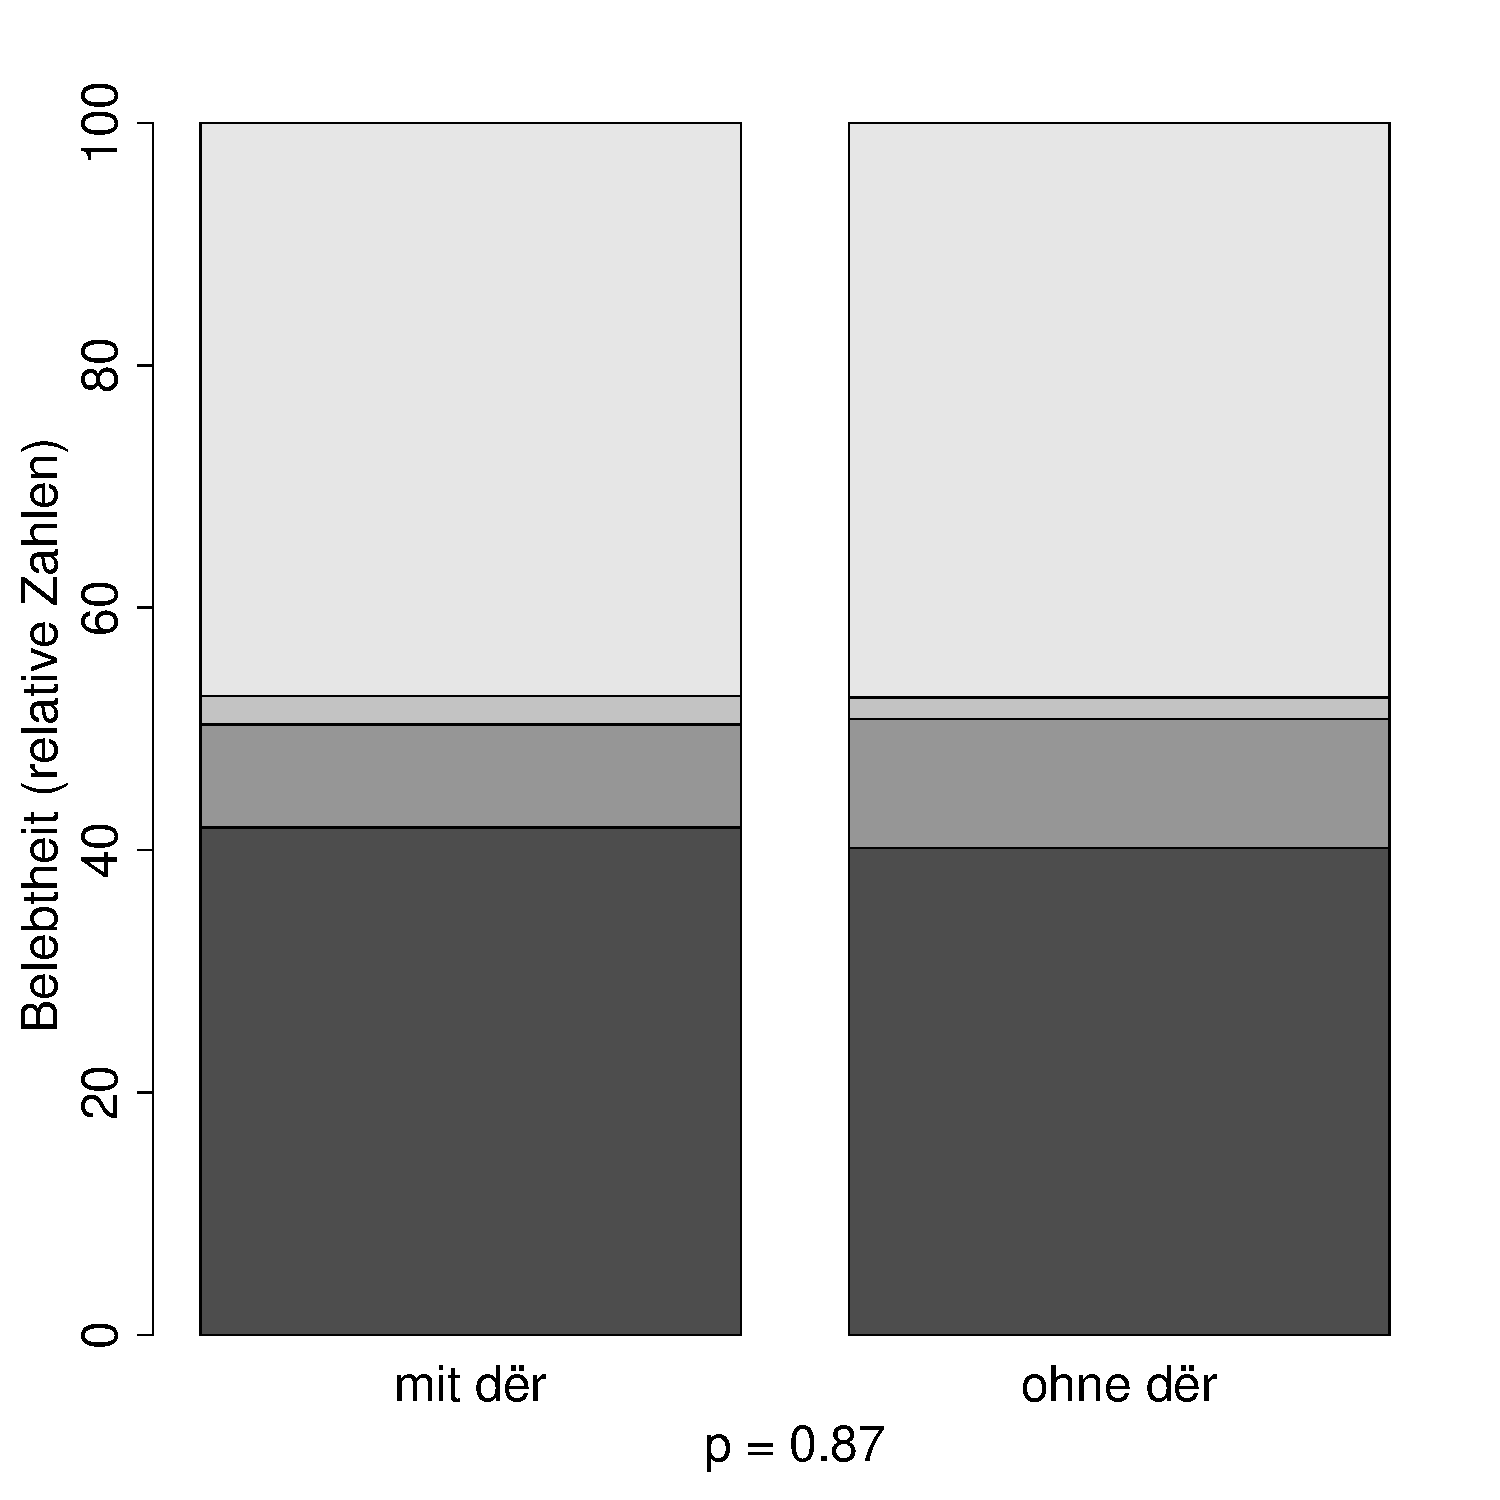
\includegraphics[height=.25\textheight]{generated/images/belebtheit-I}
\caption {Isidor}
\end{subfigure}%
\begin{subfigure}[b]{.5\linewidth}
  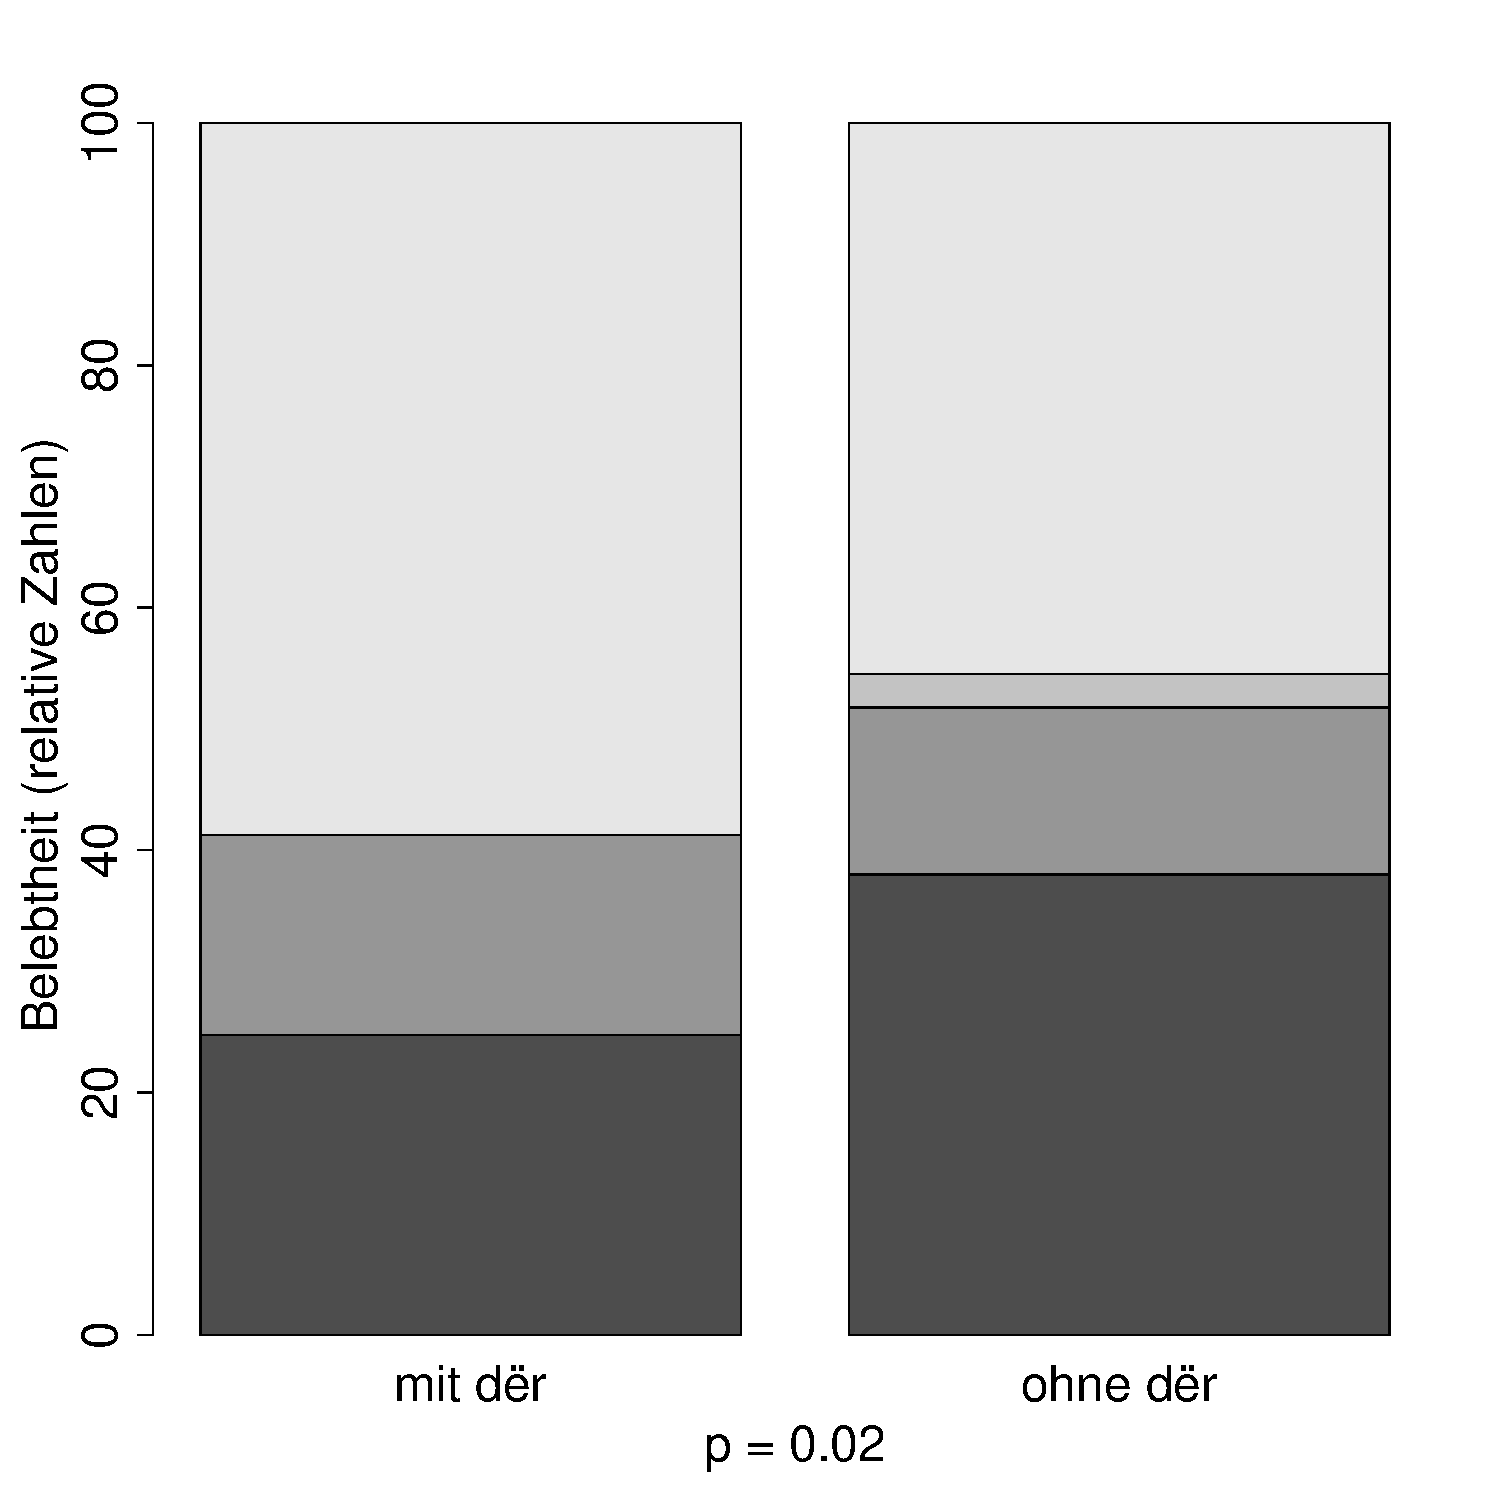
\includegraphics[height=.25\textheight]{generated/images/belebtheit-M}
\caption {Monseer Matthäus}
\end{subfigure}

\begin{subfigure}[b]{.5\linewidth}
  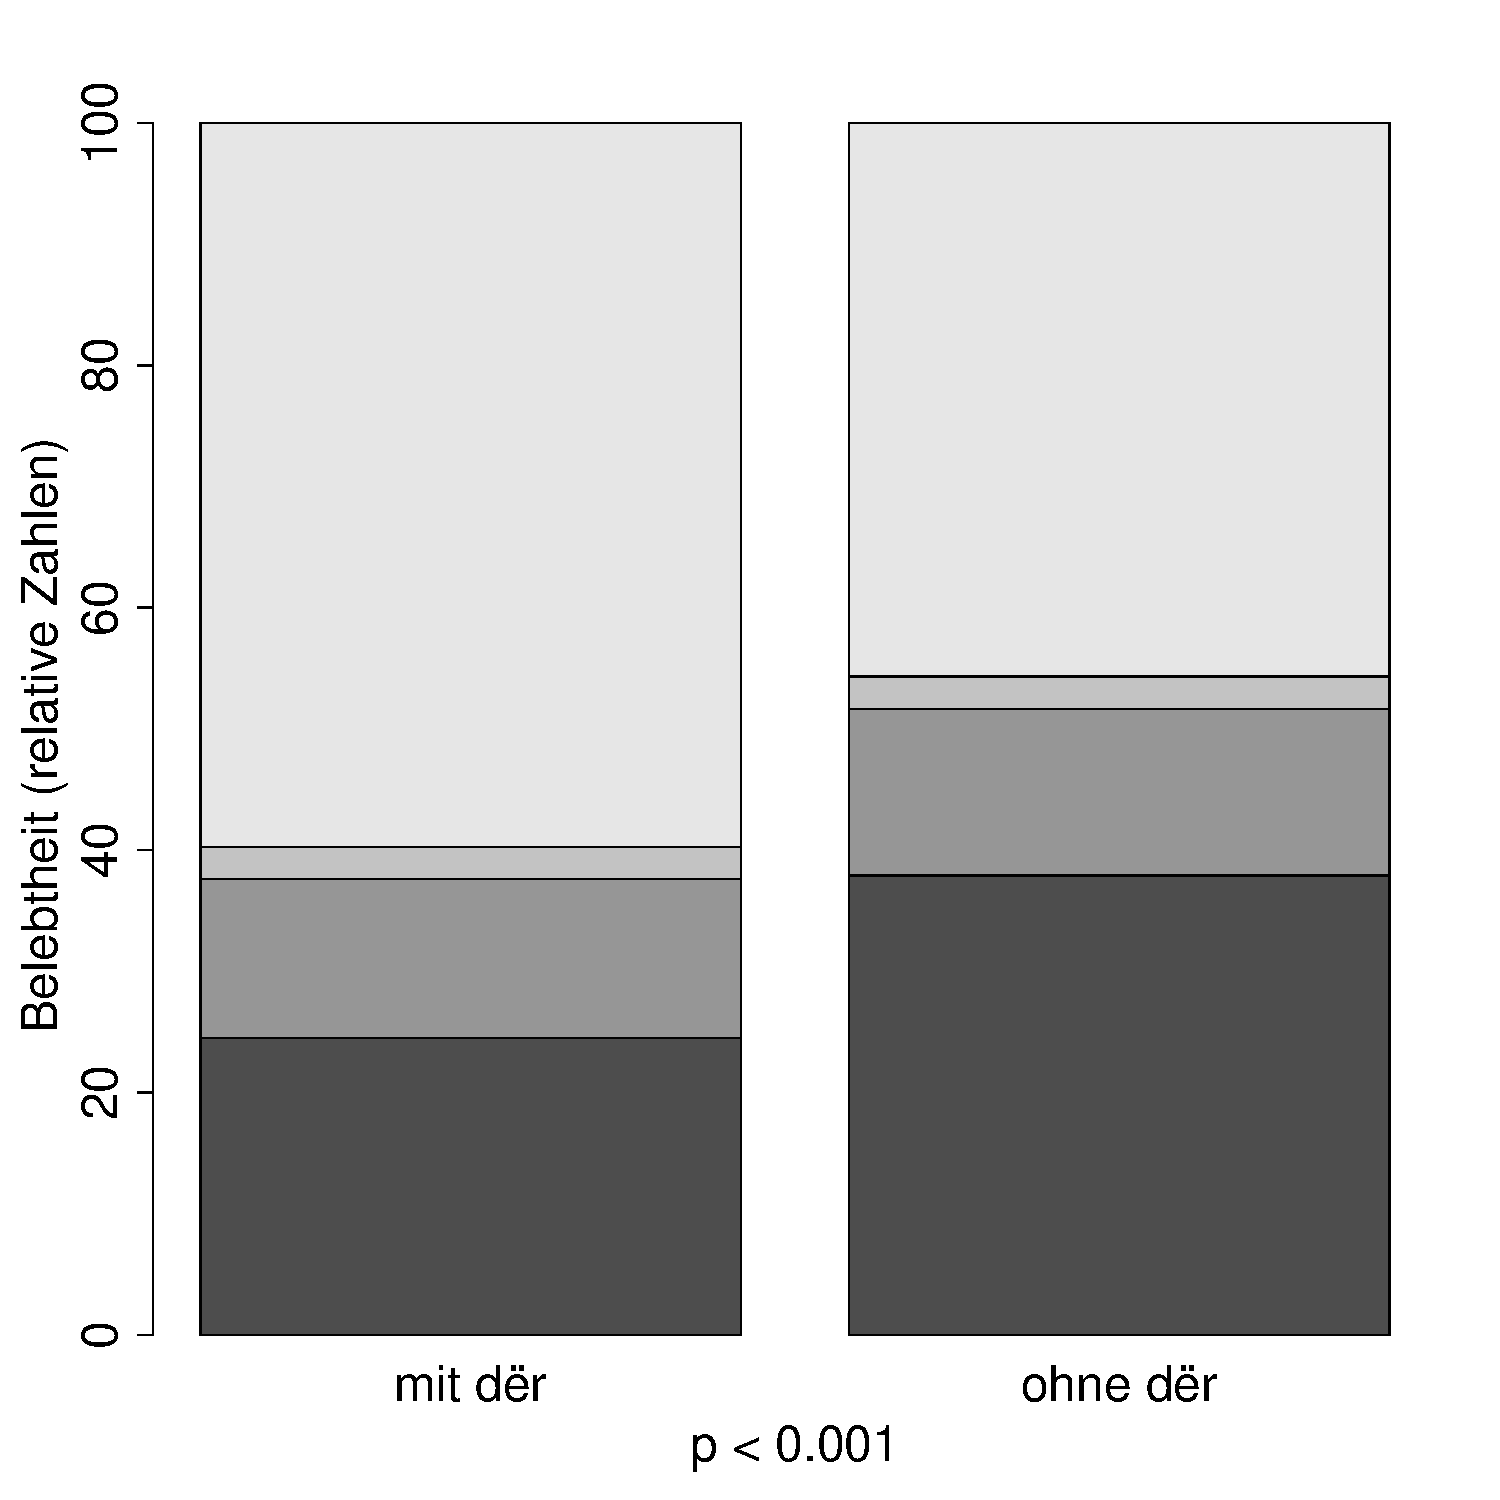
\includegraphics[height=.25\textheight]{generated/images/belebtheit-T}
\caption {Tatian}
\end{subfigure}%
\begin{subfigure}[b]{.5\linewidth}
  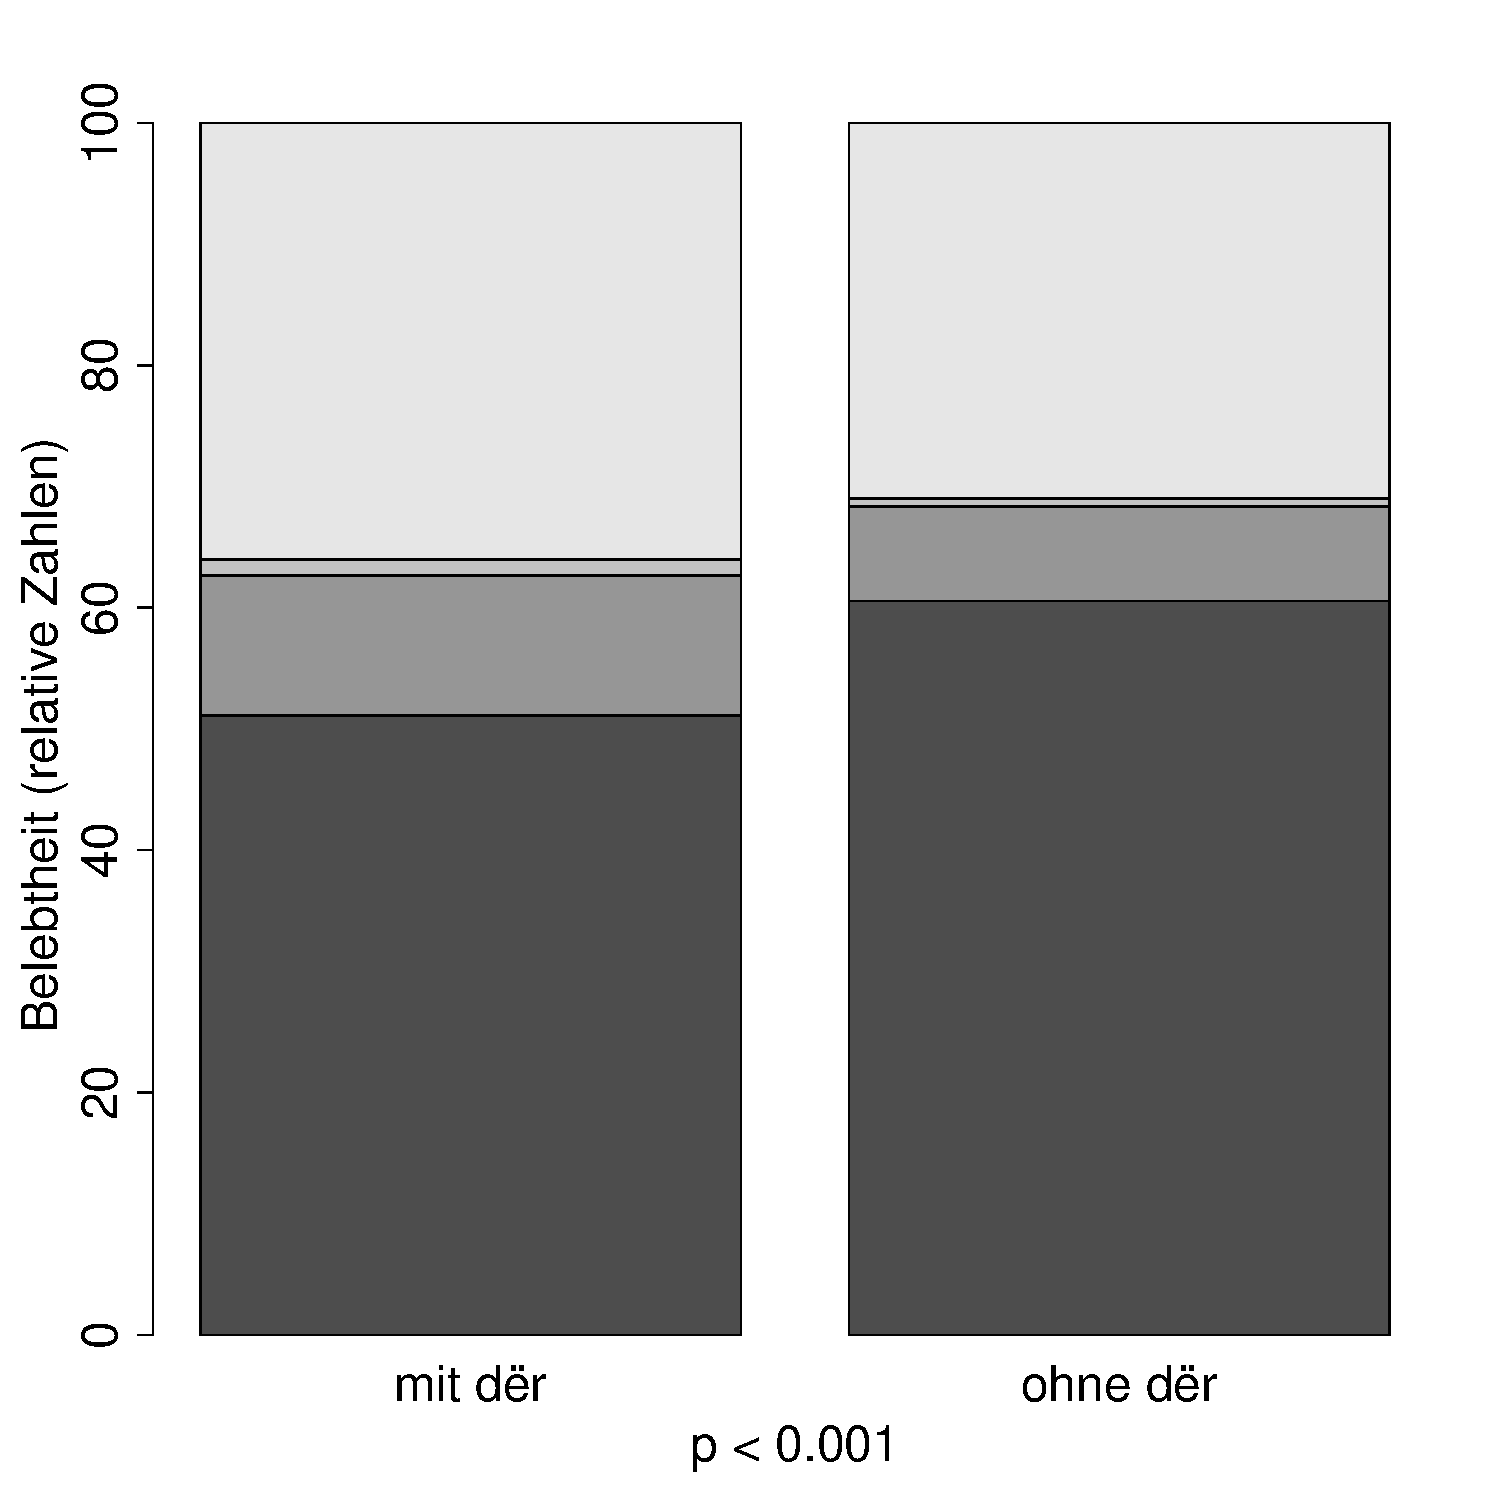
\includegraphics[height=.25\textheight]{generated/images/belebtheit-O}
\caption {Otfrid}
\end{subfigure}

\begin{subfigure}[b]{.5\linewidth}
  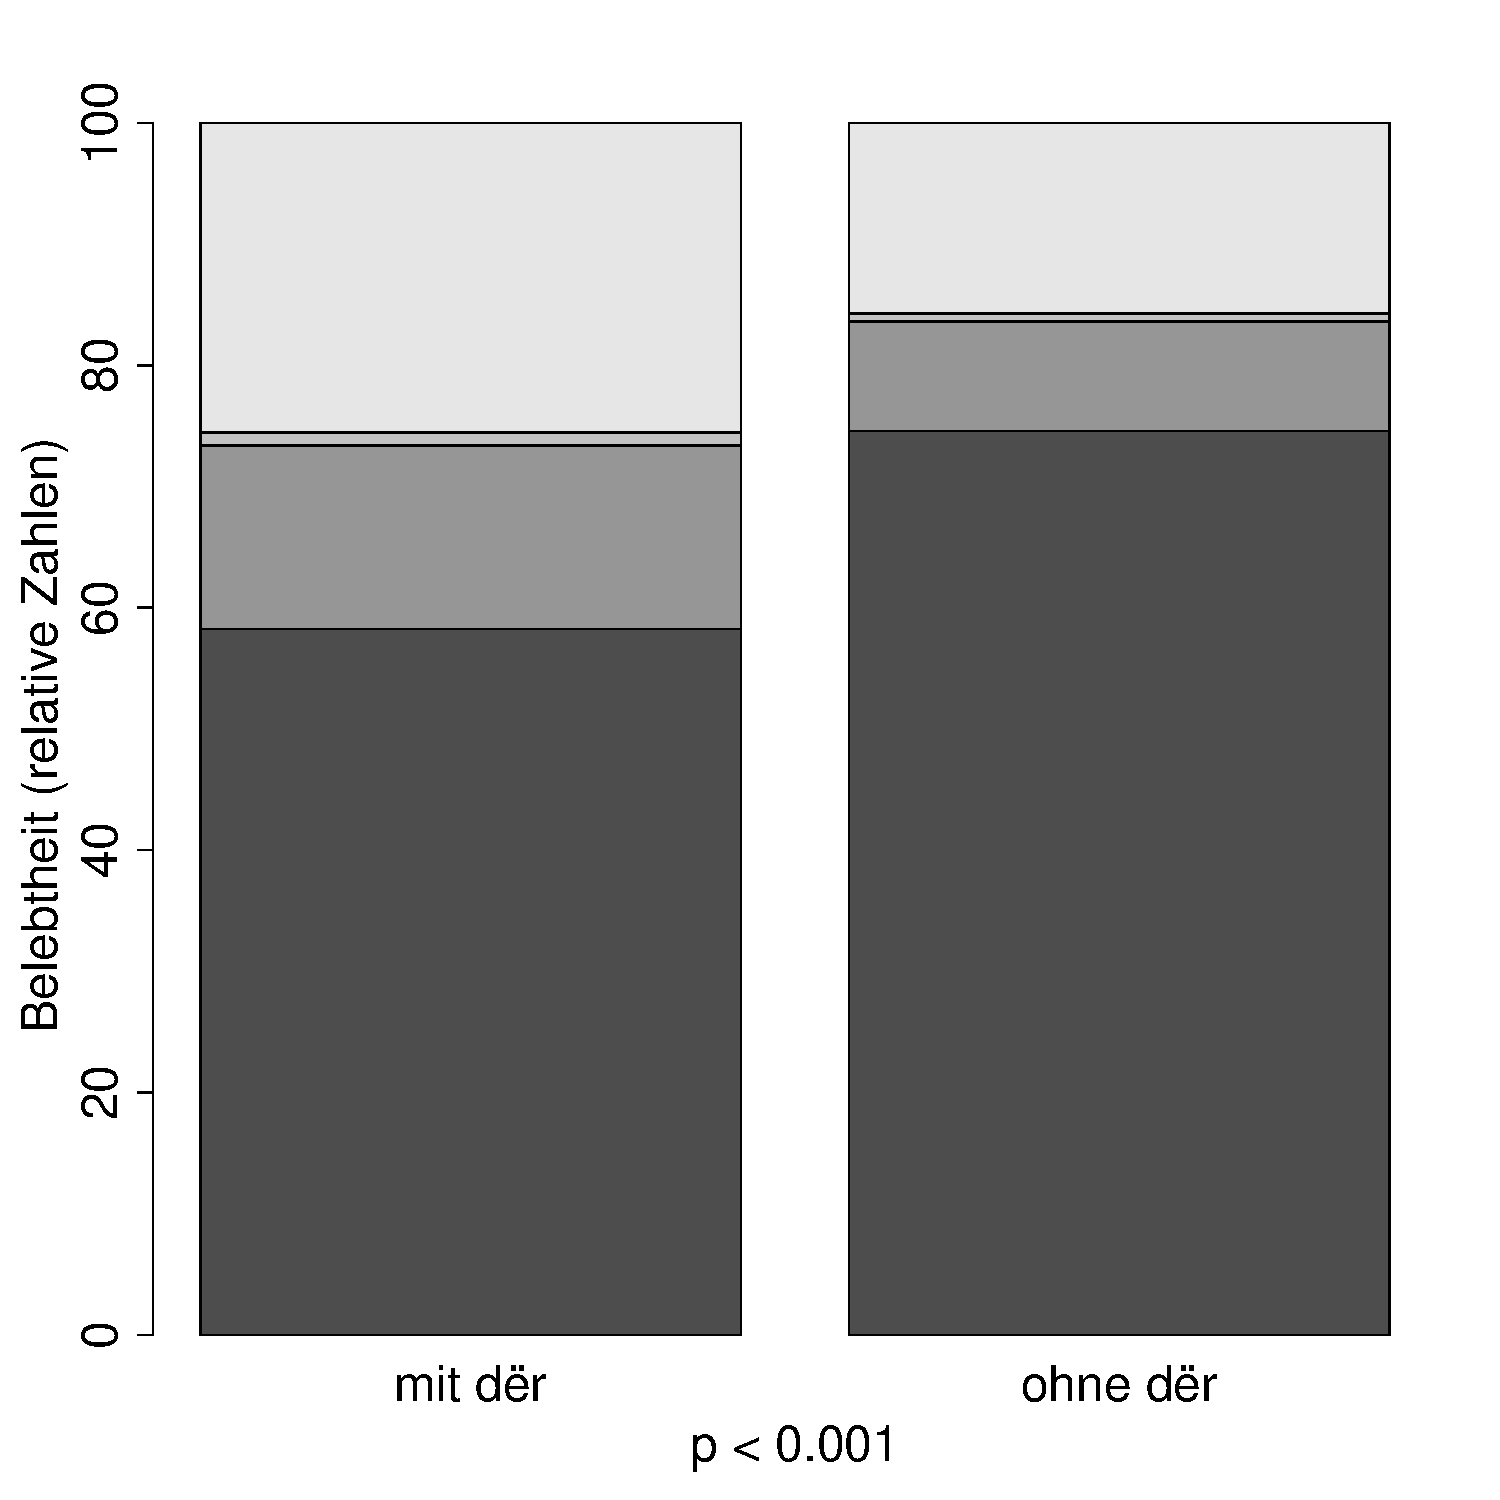
\includegraphics[height=.25\textheight]{generated/images/belebtheit-N}
\caption {Notker}
\end{subfigure}%
\begin{subfigure}[b]{.5\linewidth}
  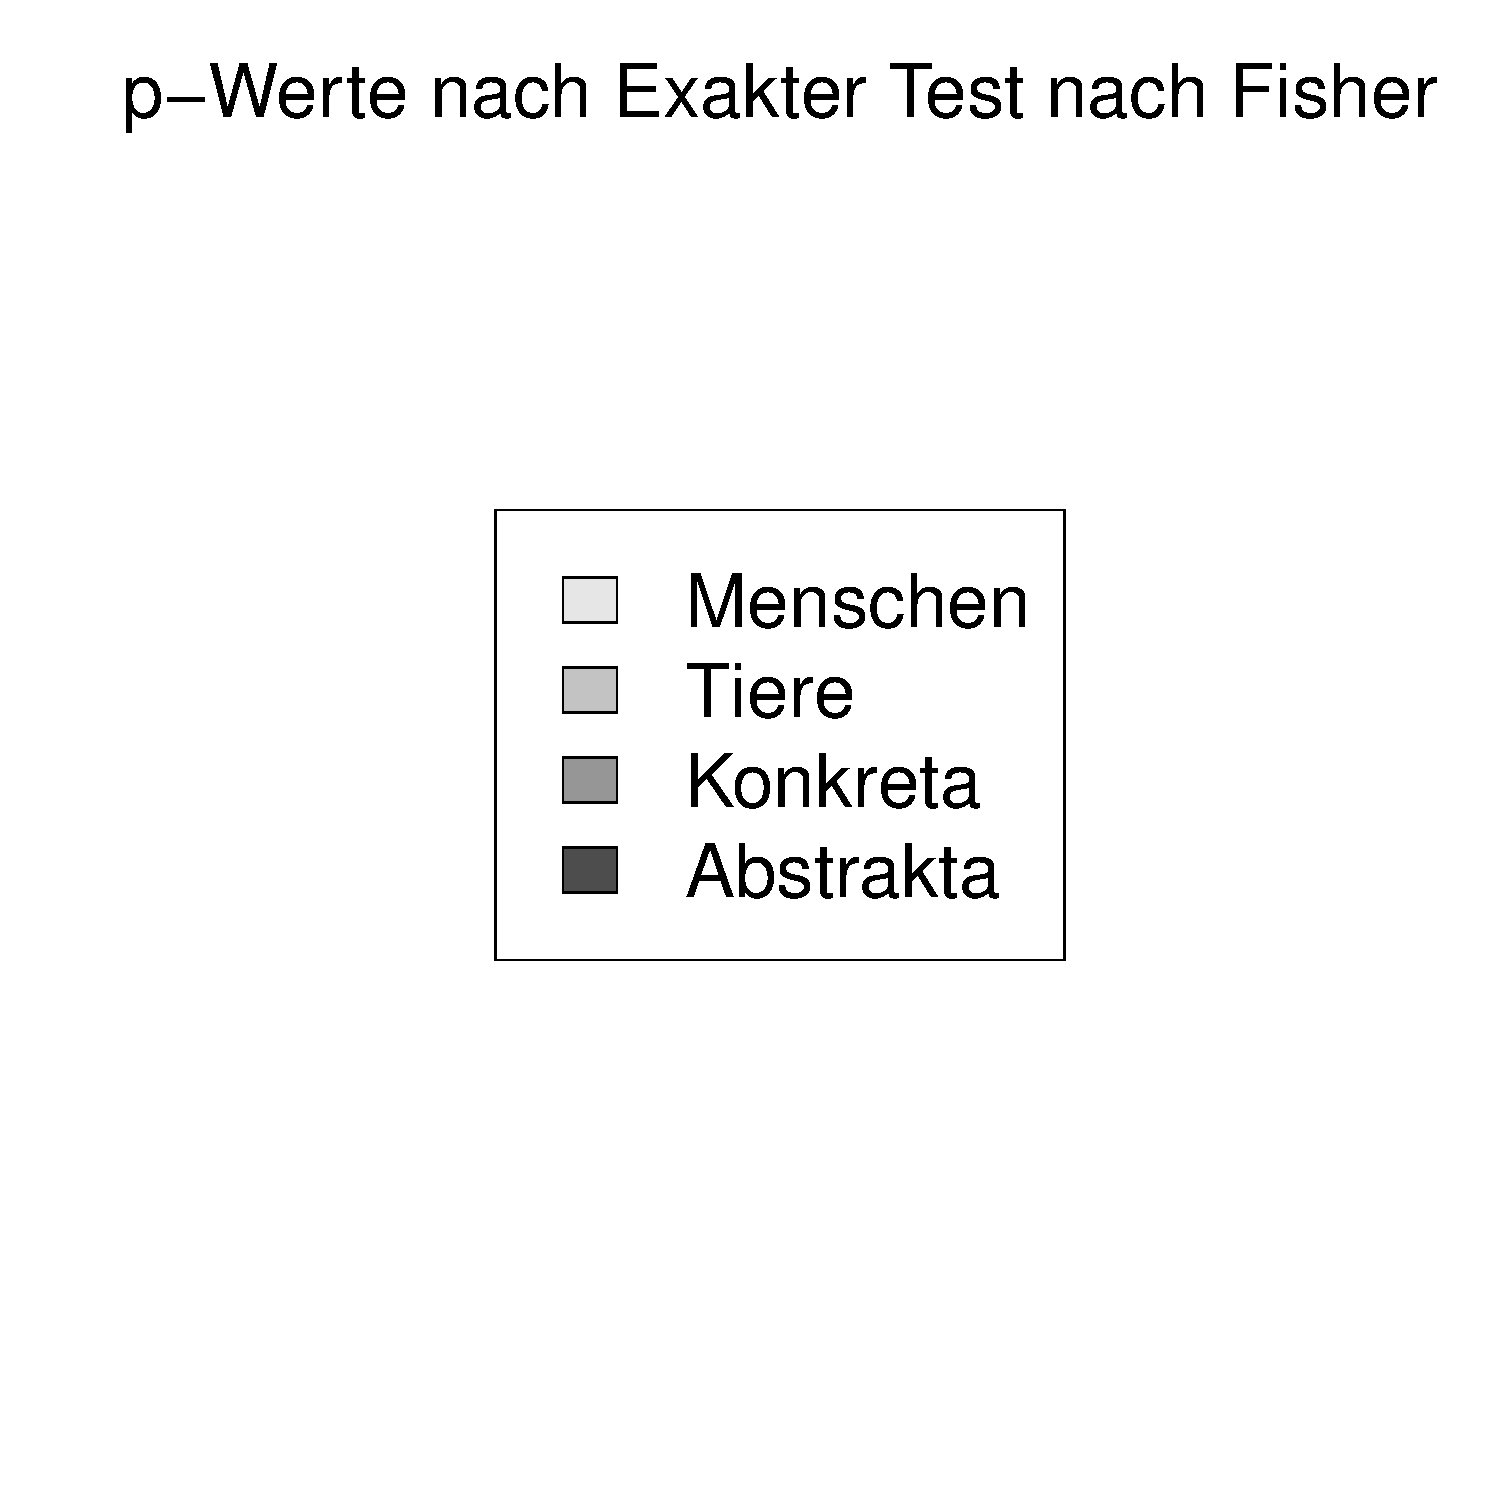
\includegraphics[height=.25\textheight]{generated/images/belebtheit-legende}
\end{subfigure}

\caption{Der Gebrauch von \object{dër} in Korrelation mit den Belebtheitsbasiskategorien}
\label{fig:bel-basis}
\end{figure}

%\inputtable{generated/tables/bel.abs-I}{Gebrauch von \object{dër} in Korrelation mit Belebtheit; \\Isidor, absolute Zahlen}{tab:I}
%\inputtable{generated/tables/bel.abs-M}{Gebrauch von \object{dër} in Korrelation mit Belebtheit; \\Monseer Matthäus, absolute Zahlen}{tab:M}
%\inputtable{generated/tables/bel.abs-T}{Gebrauch von \object{dër} in Korrelation mit Belebtheit; \\Tatian, absolute Zahlen}{tab:T}
%\inputtable{generated/tables/bel.abs-O}{Gebrauch von \object{dër} in Korrelation mit Belebtheit; \\Otfrid, absolute Zahlen}{tab:O}
%\enlargethispage{1ex}
%\inputtable{generated/tables/bel.abs-N}{Gebrauch von \object{dër} in Korrelation mit Belebtheit; \\Notker, absolute Zahlen}{tab:N}

\begin{table}
\begin{tabular}{lrrrrrr}
  \lsptoprule
{Text} & {Struktur} & {Menschen} & {Tiere} & {Konkreta} & {Abstrakta} & {Summe} \\ 
  \midrule
I & mit \object{dër} & 61 & 3 & 11 & 54 & 129 \\ 
 & ohne \object{dër} & 236 & 9 & 53 & 200 & 498 \\ 
 & Summe & 297 & 12 & 64 & 254 & 627 \\ 
   \midrule
M & mit \object{dër} & 57 & 0 & 16 & 24 & 97 \\ 
 & ohne \object{dër} & 195 & 12 & 59 & 163 & 429 \\ 
 & Summe & 252 & 12 & 75 & 187 & 526 \\ 
  \midrule
T & mit \object{dër} & 478 & 21 & 105 & 196 & 800 \\ 
 & ohne \object{dër} & 1333 & 78 & 402 & 1106 & 2919 \\ 
 & Summe & 1811 & 99 & 507 & 1302 & 3719 \\ 
  \midrule
O & mit \object{dër} & 698 & 25 & 224 & 990 & 1937 \\ 
 & ohne \object{dër} & 1490 & 33 & 375 & 2912 & 4810 \\ 
 & Summe & 2188 & 58 & 599 & 3902 & 6747 \\ 
  \midrule
N & mit \object{dër} & 96 & 4 & 57 & 219 & 376 \\ 
 & ohne \object{dër} & 174 & 7 & 100 & 825 & 1106 \\ 
 & Summe & 270 & 11 & 157 & 1044 & 1482 \\ 
   \lspbottomrule
\end{tabular}
\caption{Gebrauch von \object{dër} in Korrelation mit \isi{Belebtheit} (absolute Zahlen)}
\label{tab:bel-abs}
\end{table}

Um zu überprüfen, inwiefern die Häufigkeiten in den einzelnen Kategorien von einer zufälligen Verteilung abweichen, wurden die \hervor{Pearson residuals} \parencite{Gries2012} errechnet. Die Nullhypothese, auf denen die Residuen in Abbildung~\ref{fig:residuals-bel}\footnote{ 
Die Mosaikplots sind folgendermaßen zu lesen: Auf der horizontalen Achse sind die Belege in Appellativa \is{Gattungsname} mit und ohne \object{dër} aufgeteilt. Vertikal sieht man die Anteile der menschlichen, tierischen, konkreten und abstrakten Referenten in diesen Gruppen. Die Einfärbung sowie die Strichart zeigt an, ob eine Belebtheitskategorie \is{Belebtheit} häufiger als erwartet mit bzw. ohne \object{dër} erscheint: Eine blaue Einfärbung mit durchgezogener Umrandung steht für eine Abweichung, die größer ist als erwartet, eine rote Einfärbung mit gestrichelter Linie zeigt an, dass die Abweichung niedriger als erwartet ist -- beides jeweils im Vergleich zu den Nachbarzellen. Je dunkler der Farbton, umso größer ist die Abweichung. Weiße Kästen mit gestrichelten bzw. durchgezogenen Linien spiegeln Tendenzen, aber keine Signifikanz (vgl. auch die Legende an der Seite der Grafiken).} basieren, lautet: Die \isi{Belebtheit} hat keinen Einfluss auf die Setzung von \object{dër}. 

Bei Isidor und dem Monseer Matthäus erlauben es die Daten nicht, die Nullhypothese abzulehnen. Es lässt sich kein Einfluss von der Belebtheitskategorie \is{Belebtheit} auf die Artikelsetzung feststellen. Dennoch sieht man in den Monseer Fragmenten eine leichte Affinität von konkreten und menschlichen Referenten zu \object{dër}. Dass im Isidor die Abstrakta \is{Abstraktum} leichter zur \object{dër}-Setzung tendieren als die \is{Konkretum} Konkreta, liegt vermutlich am Thema: Häufig wird auf abstrakte, biblische Referenten wie \object{drinissa} (\extrans{Dreieinigkeit}) oder  \object{megin} (\extrans{Gewalt, Macht}) verwiesen.
 
Im Tatian ist hingegen deutlich zu sehen, dass menschliche Referenten überzufällig häufiger mit \object{dër} determiniert werden als \is{Abstraktum} Abstrakta. Die Abweichungen sind, wie der Fisher Test (Abbildung \ref{fig:bel-basis}) zeigt, auch signifikant. Bei Otfrid neigen nicht nur Menschen, sondern auch  Tierbezeichnungen und Konkreta \is{Konkretum} stärker zur \object{dër}-Setzung. Ein ähnliches Bild zeigt sich bei Notker. Hier ist der Einfluss von \isi{Belebtheit} nicht mehr so stark, aber immer noch signifikant.    

Damit ausgeschlossen werden kann, dass frequente Lemmata \is{Lemma} den Anteil einer Kategorie nach oben treiben und damit das Bild verzerren, wurden die Hapax Legomena separat ausgewertet, s. Abbildung~\ref{fig:residuals-bel-hapaxe}. Bemerkenswert ist, dass nun auch dem Isidor ein höherer Anteil belebter Referenten bei den \object{dër}-Belegen attestiert werden kann. Bei den anderen Denkmälern hat sich mit Ausnahme von Notker das Bild wenig geändert. 

Auch für diese Verteilung wurden Residuen errechnet, s. Abbildung~\ref{fig:bel-hapaxe-residuals}. Es fällt auf, dass bei Otfrid die belebten Referenten signifikant häufiger in der \object{dër}-Gruppe erscheinen als in der Gruppe ohne \object{dër} ($p = 0{,}01$). In den anderen Texten spiegeln die Residuen zwar eine Tendenz, dass belebte und konkrete Referenten häufiger mit \object{dër}-auftreten; die Verteilung ist aber nicht signifikant (vgl. die $p$-Werte in Abbildung~\ref{fig:bel-hapaxe}). Einzig bei Notker, dem jüngsten Text, zeigt sich kein positiver \is{Belebtheit} Belebtheitseffekt. Die Tendenz geht sogar in die andere Richtung: Belebte Hapaxe werden eher nicht mit \object{dër} determiniert. Diese Verteilung ist allerdings nicht signifikant ($p = 0{,}68$).  

\begin{figure}
\begin{subfigure}[b]{.5\linewidth}
  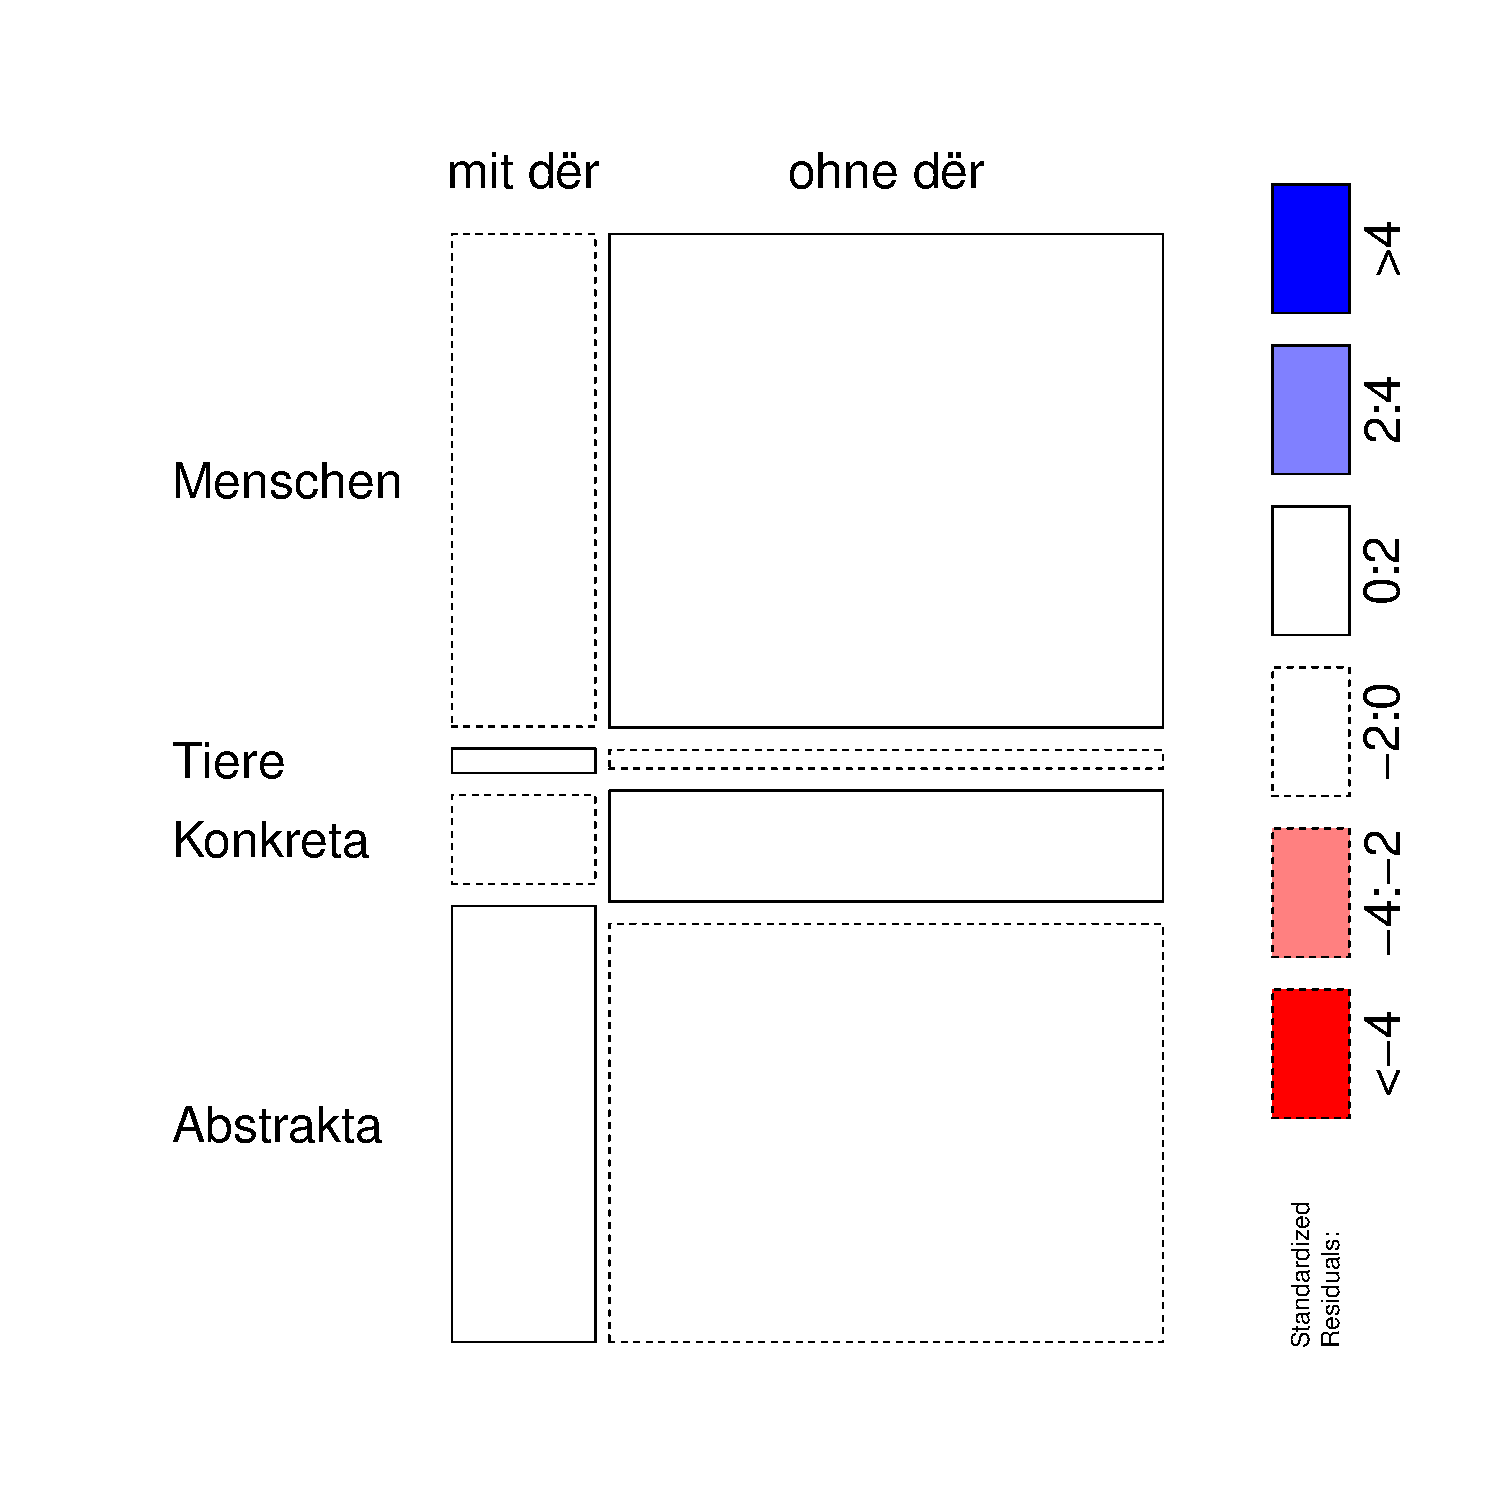
\includegraphics[height=.25\textheight]{generated/images/residuals-bel-I}
\caption {Isidor}
\end{subfigure}%
\begin{subfigure}[b]{.5\linewidth}
  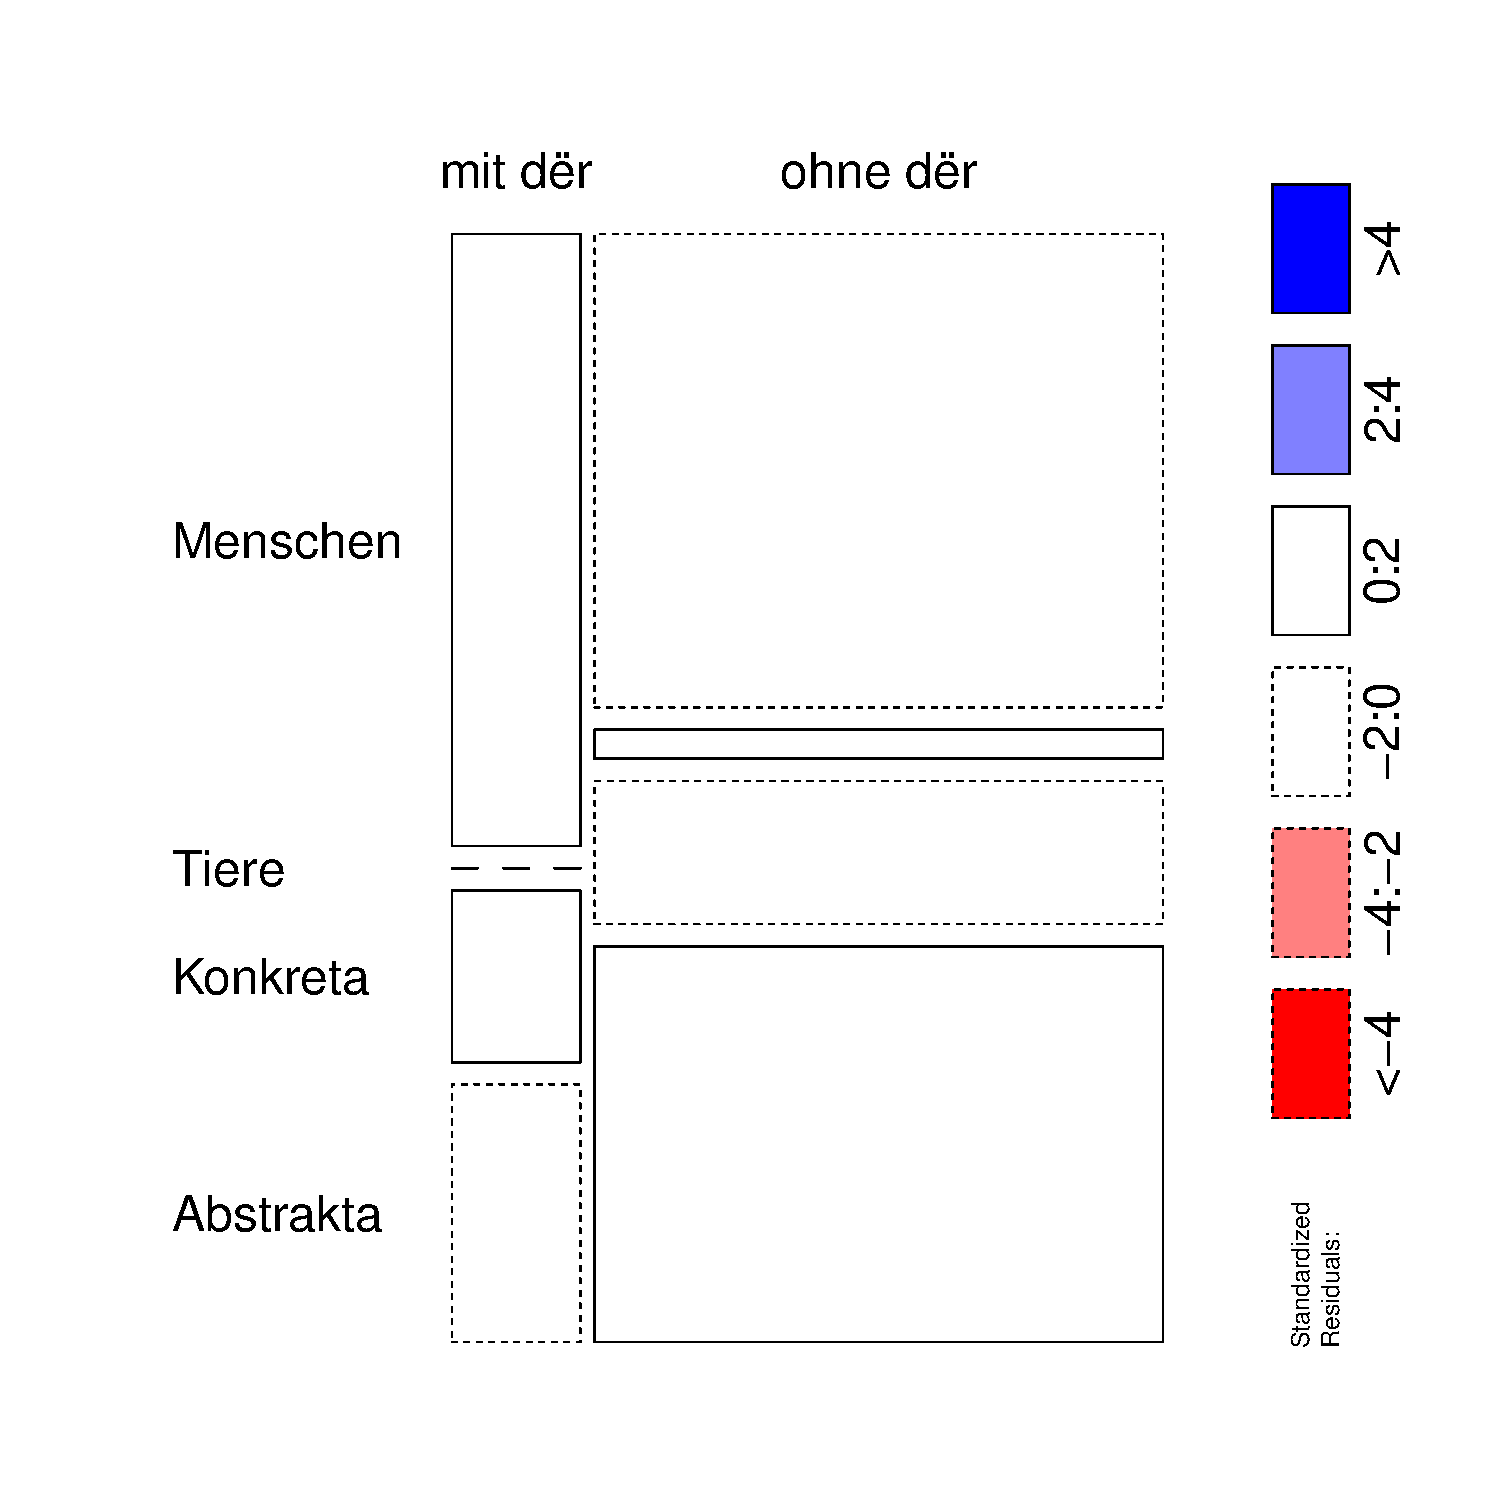
\includegraphics[height=.25\textheight]{generated/images/residuals-bel-M}
\caption {Monseer Matthäus}
\end{subfigure}

\begin{subfigure}[b]{.5\linewidth}
  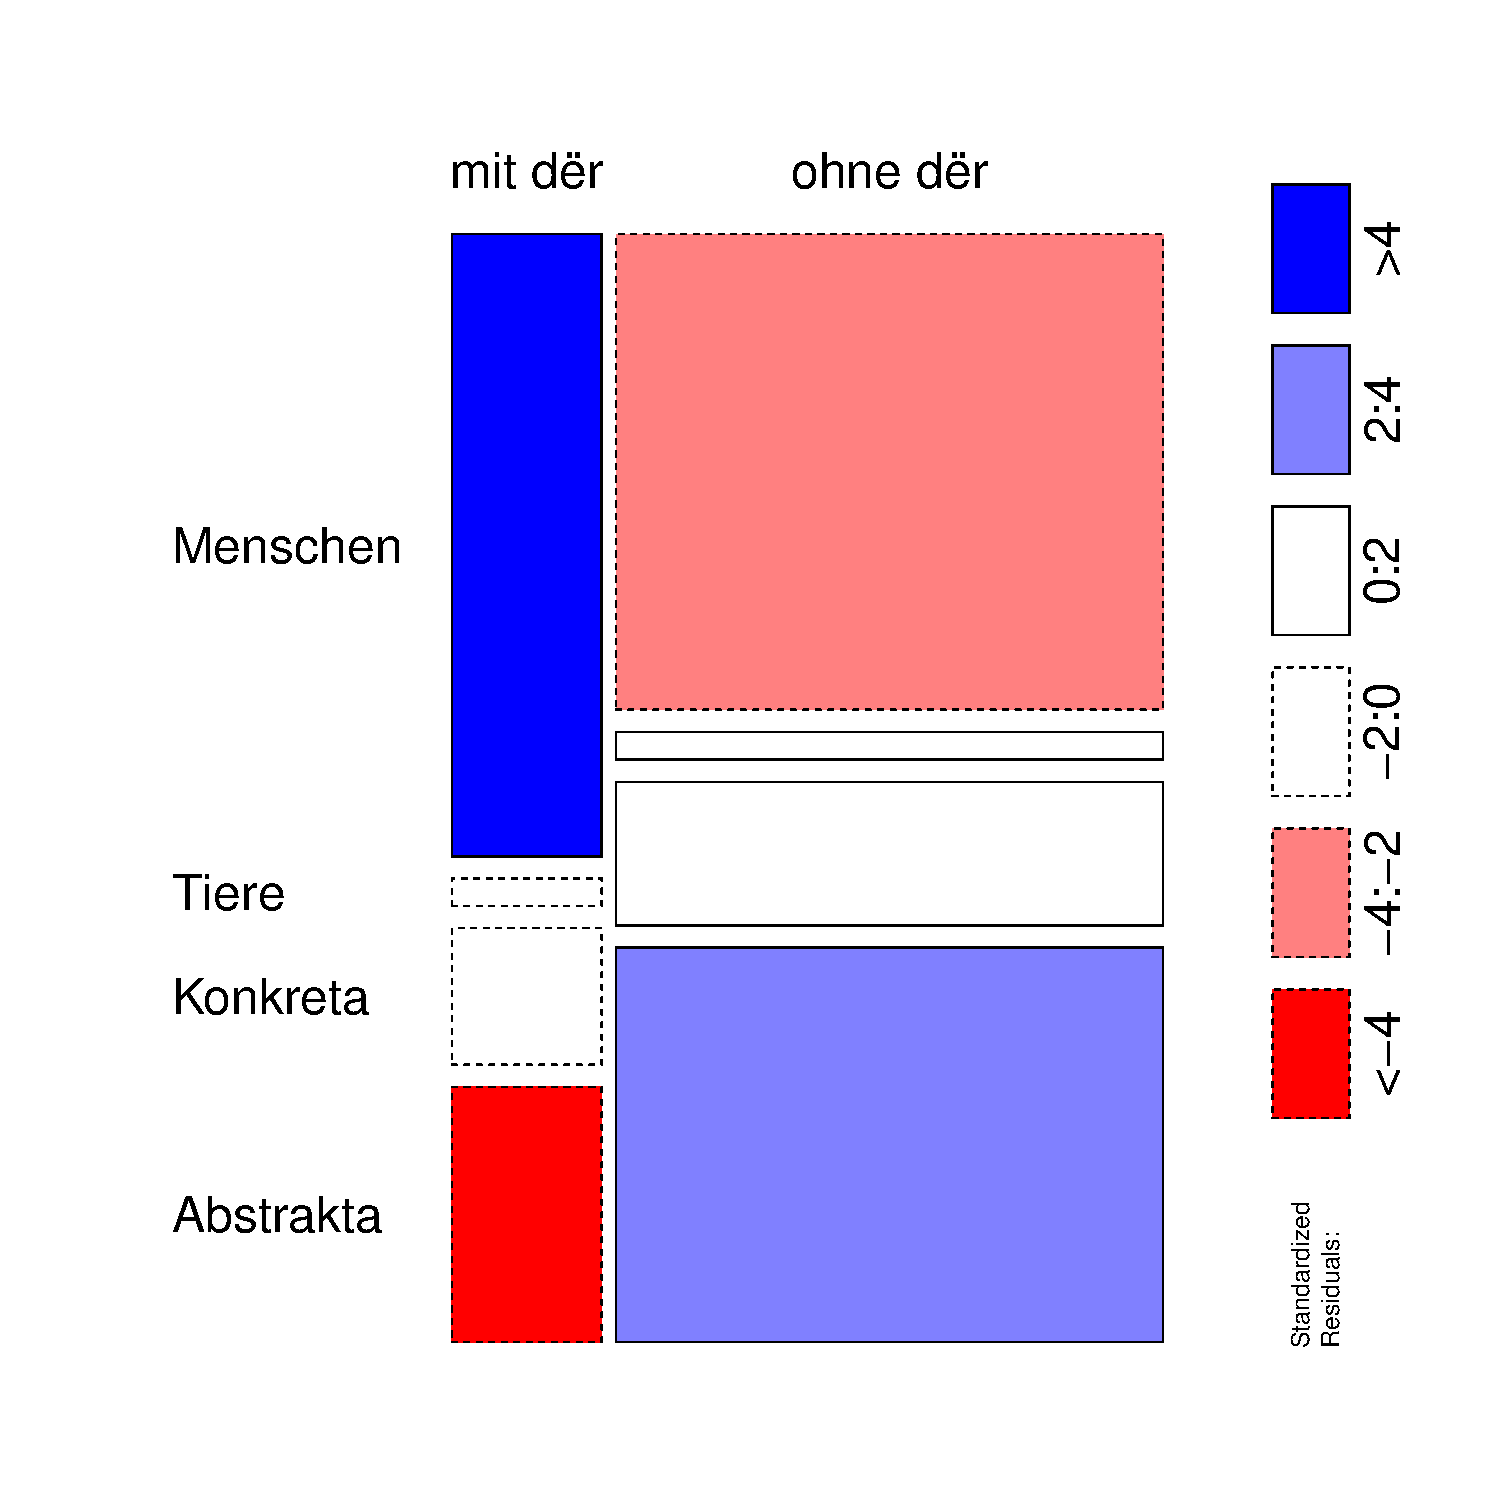
\includegraphics[height=.25\textheight]{generated/images/residuals-bel-T}
\caption {Tatian}
\end{subfigure}%
\begin{subfigure}[b]{.5\linewidth}
  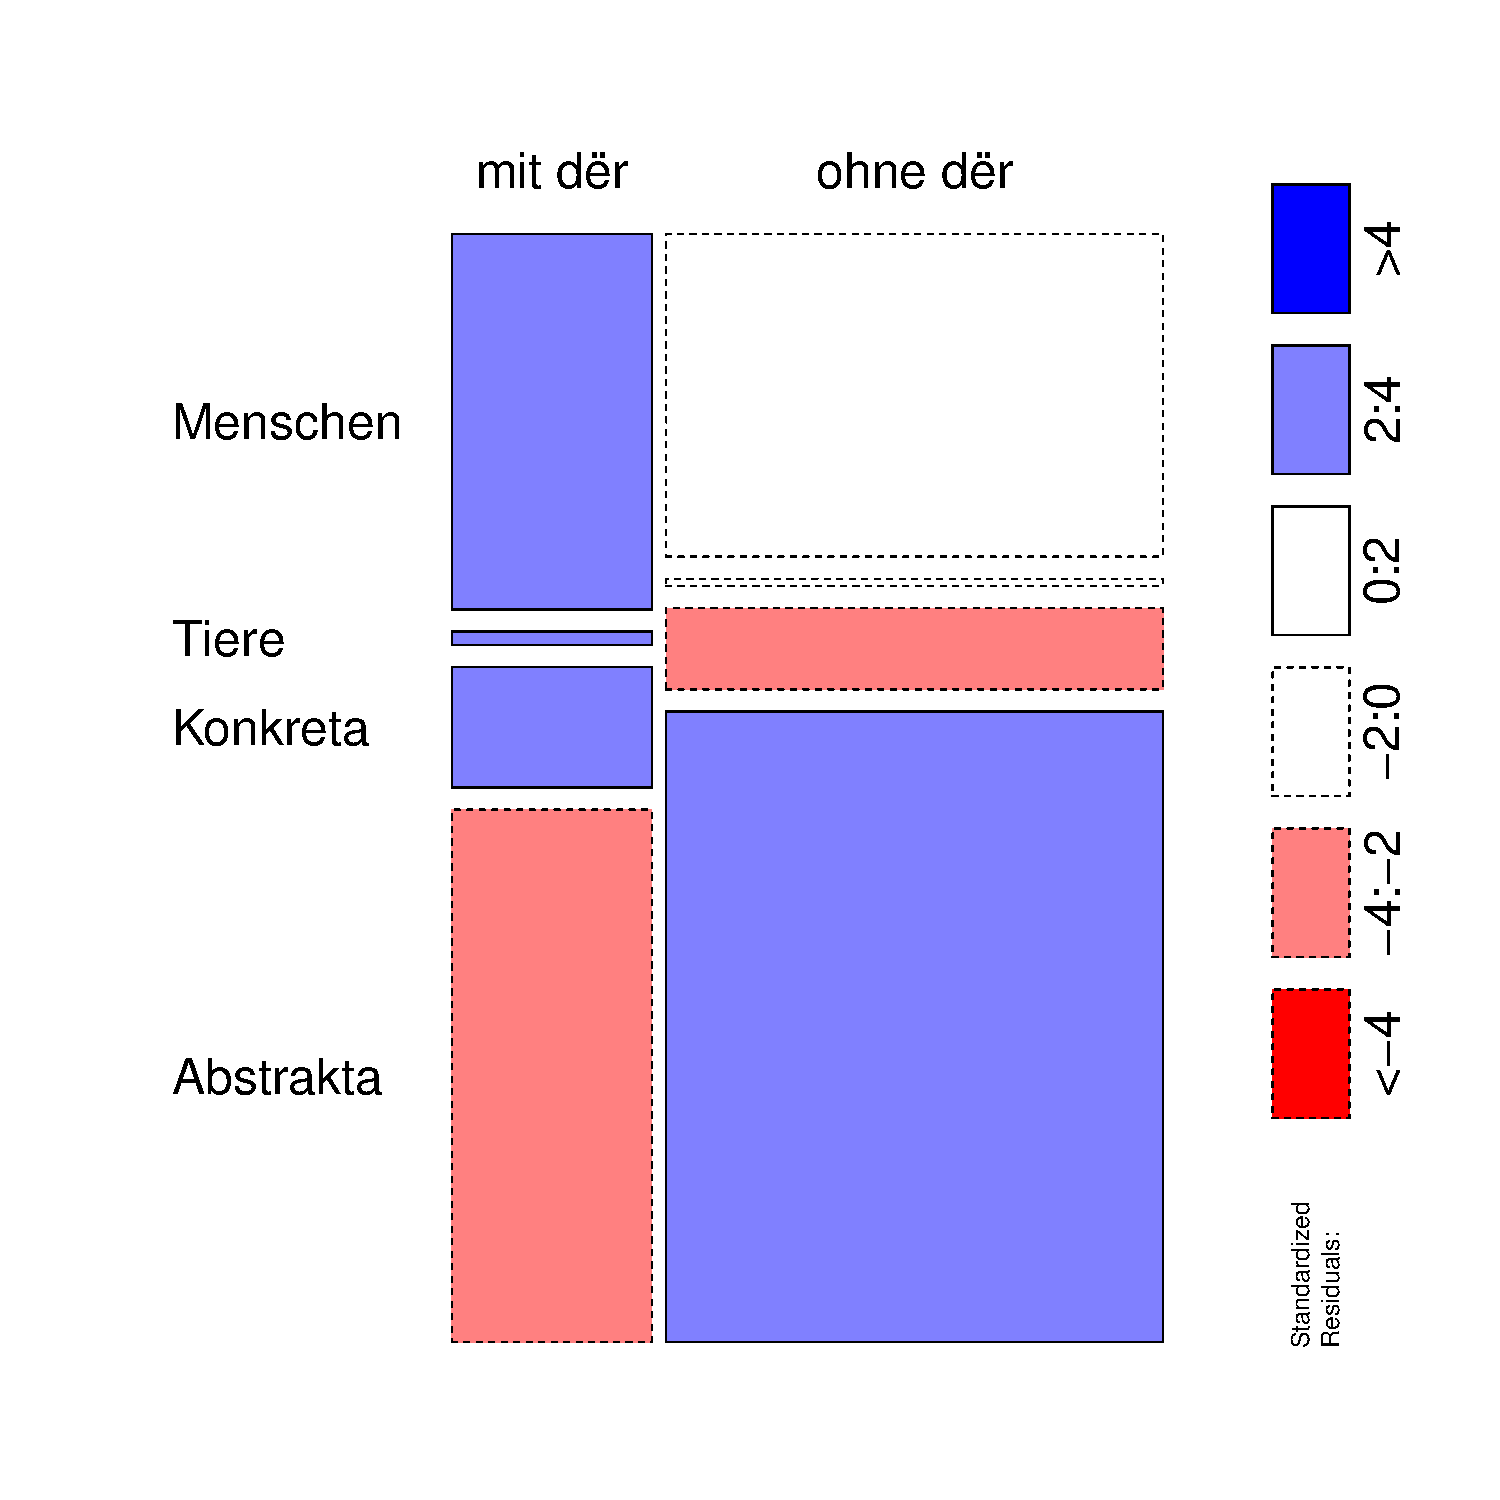
\includegraphics[height=.25\textheight]{generated/images/residuals-bel-O}
\caption {Otfrid}
\end{subfigure}

\begin{subfigure}[b]{.5\linewidth}
  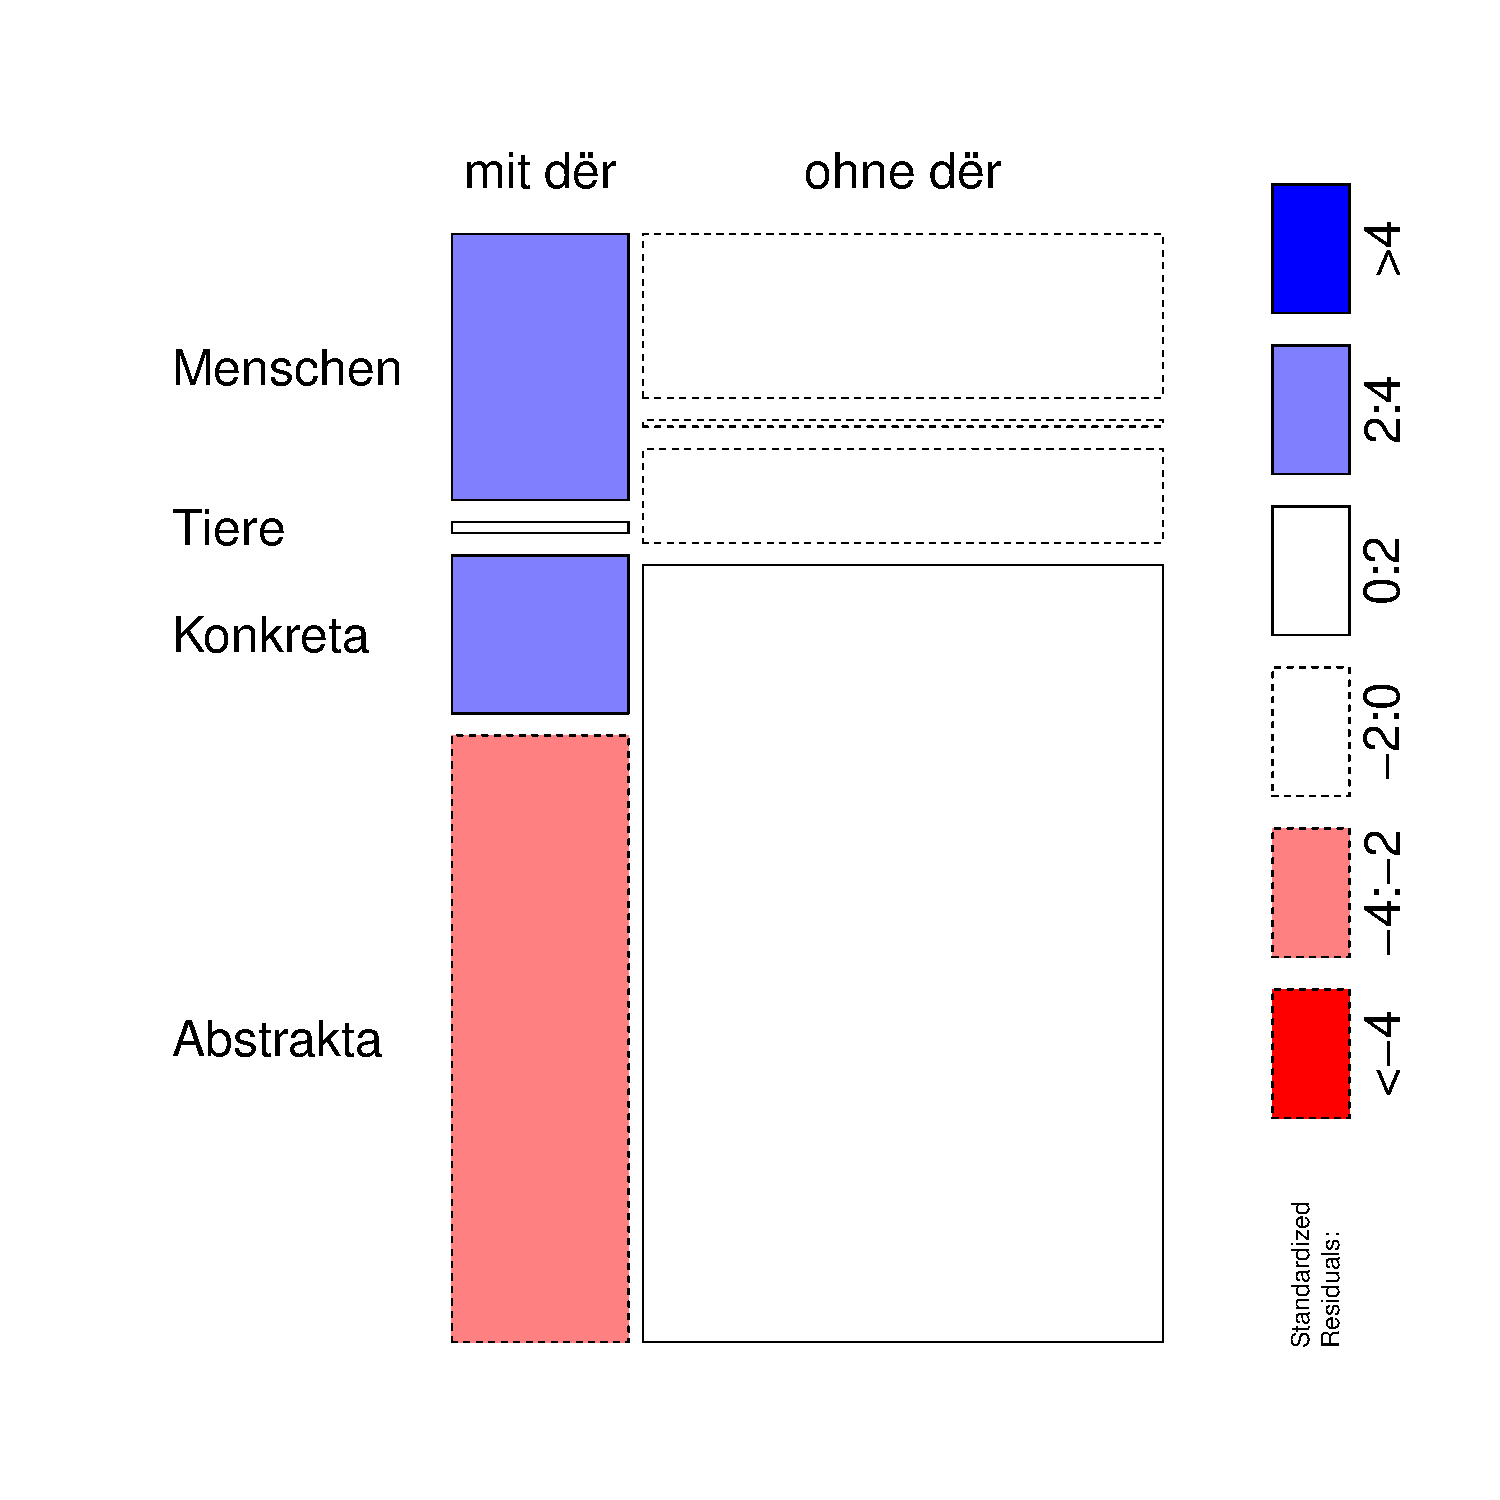
\includegraphics[height=.25\textheight]{generated/images/residuals-bel-N}
\caption {Notker}
\end{subfigure}
\caption{Einfluss von Belebtheit auf \object{dër}-Gebrauch (Residuen)}
\label{fig:residuals-bel}
\end{figure}


\begin{figure}
\begin{subfigure}[b]{.5\linewidth}
  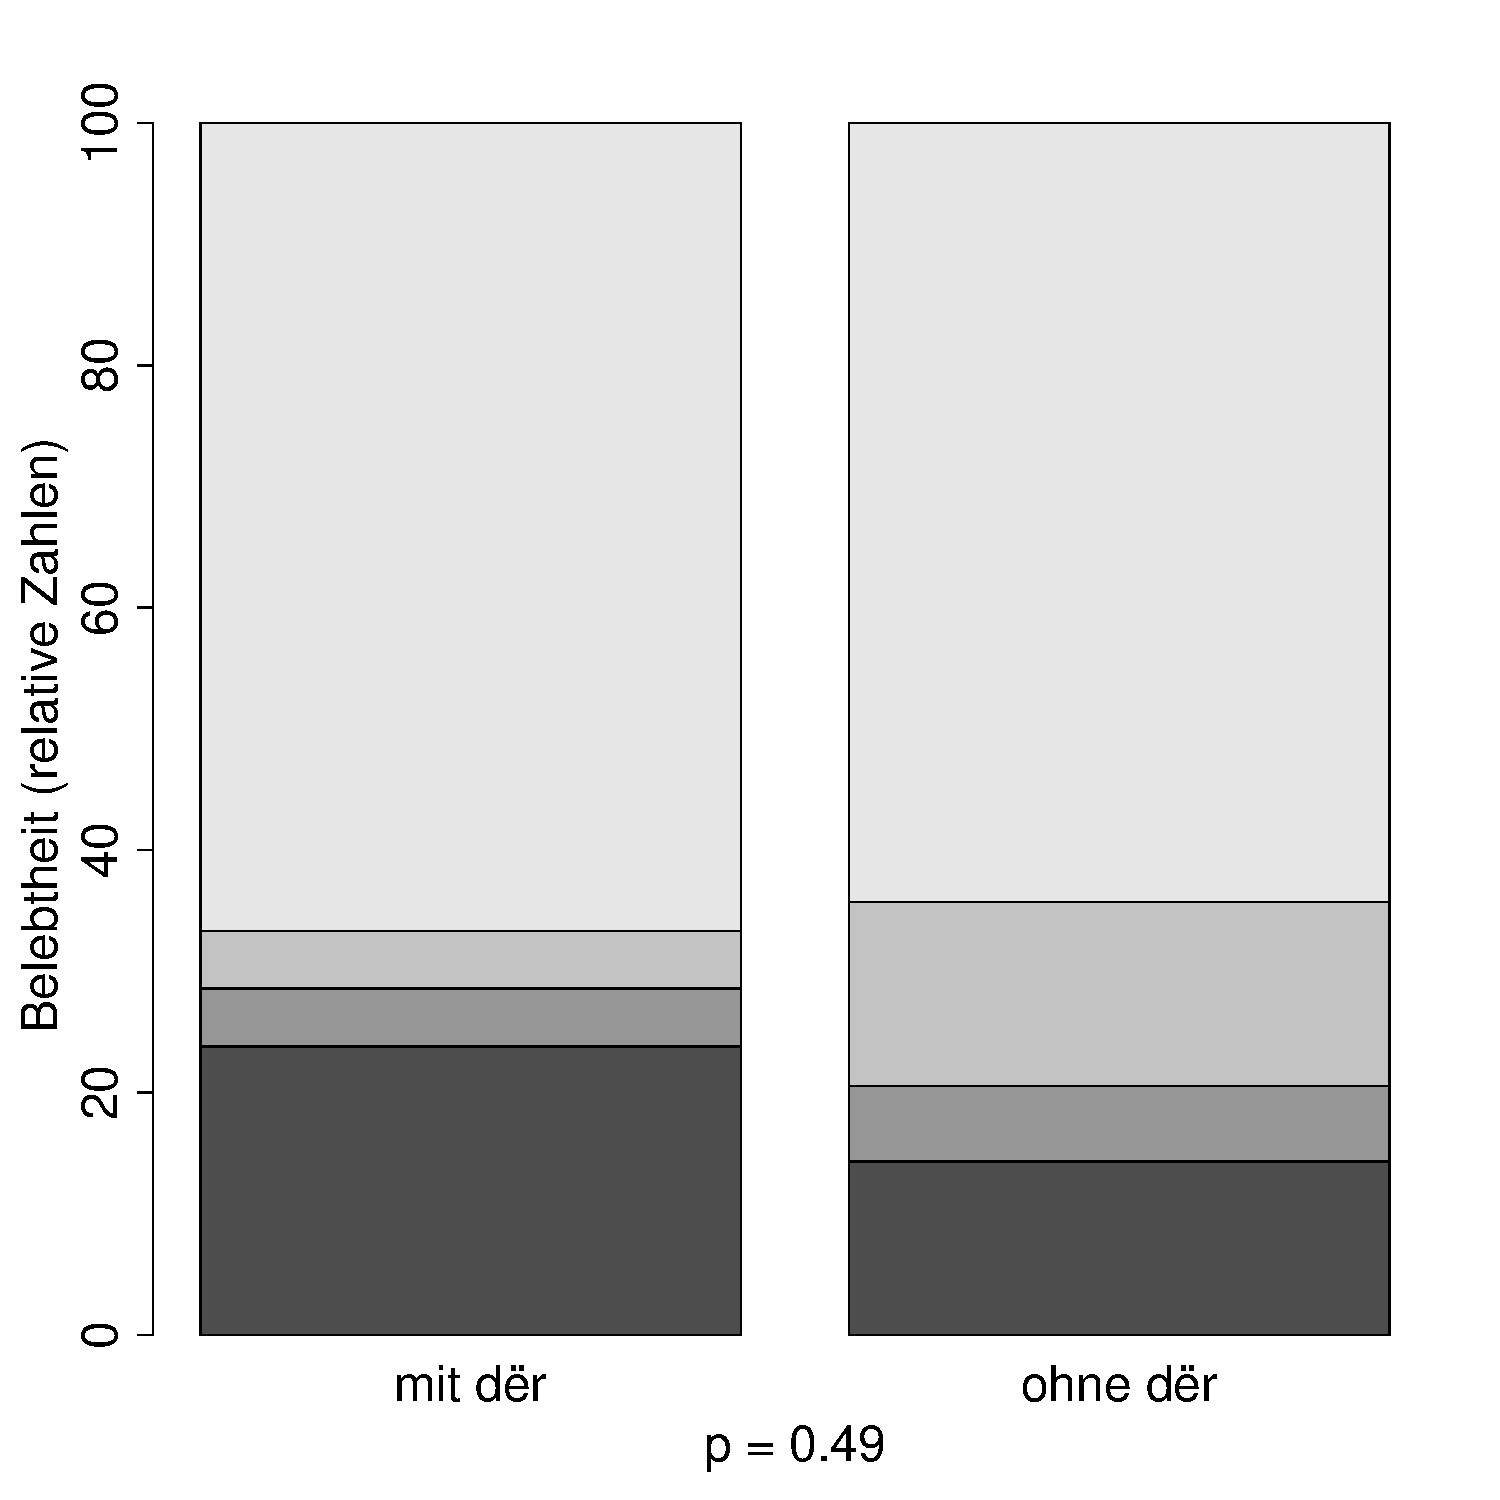
\includegraphics[height=.25\textheight]{generated/images/belebtheit-hapaxe-I}
\caption {Isidor}
\end{subfigure}%
\begin{subfigure}[b]{.5\linewidth}
  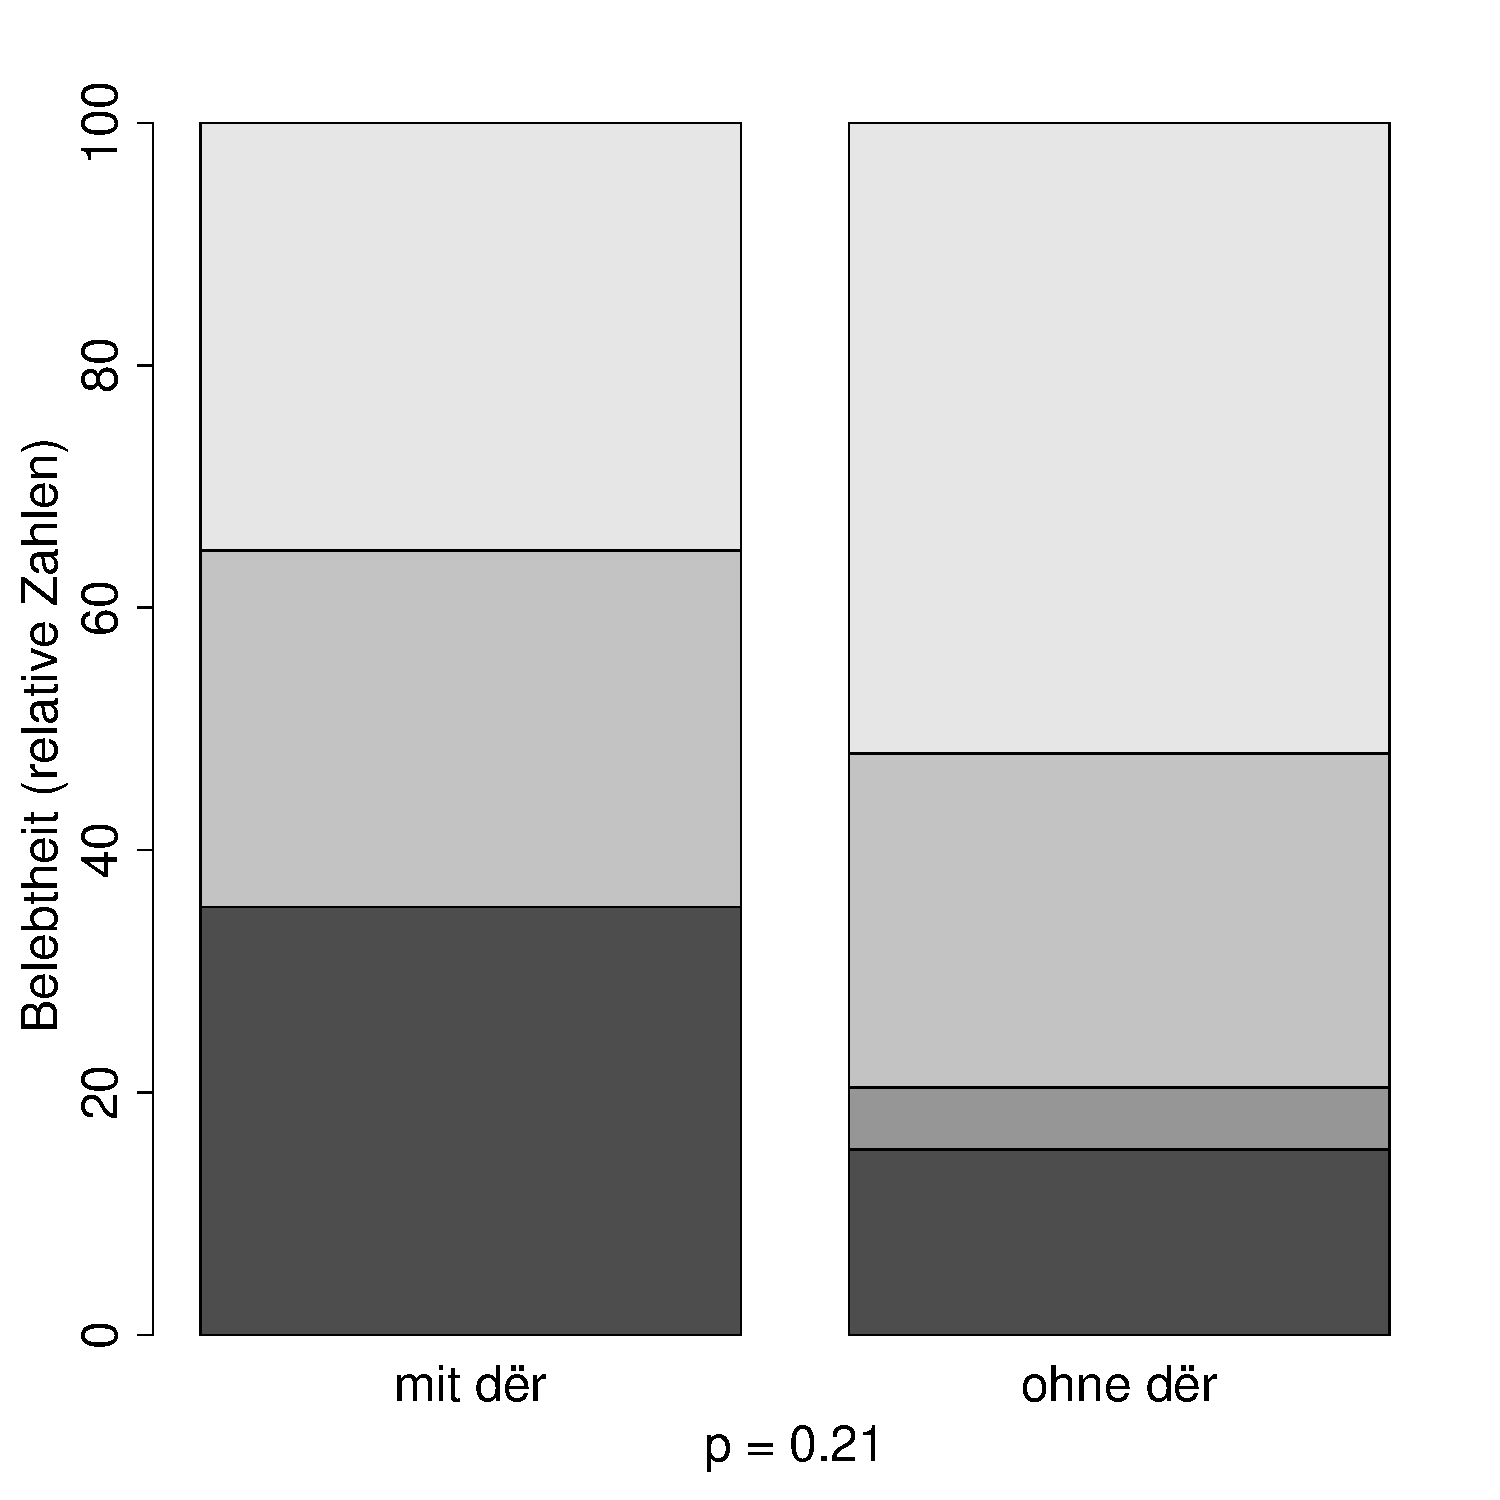
\includegraphics[height=.25\textheight]{generated/images/belebtheit-hapaxe-M}
\caption {Monseer Matthäus}
\end{subfigure}

\begin{subfigure}[b]{.5\linewidth}
  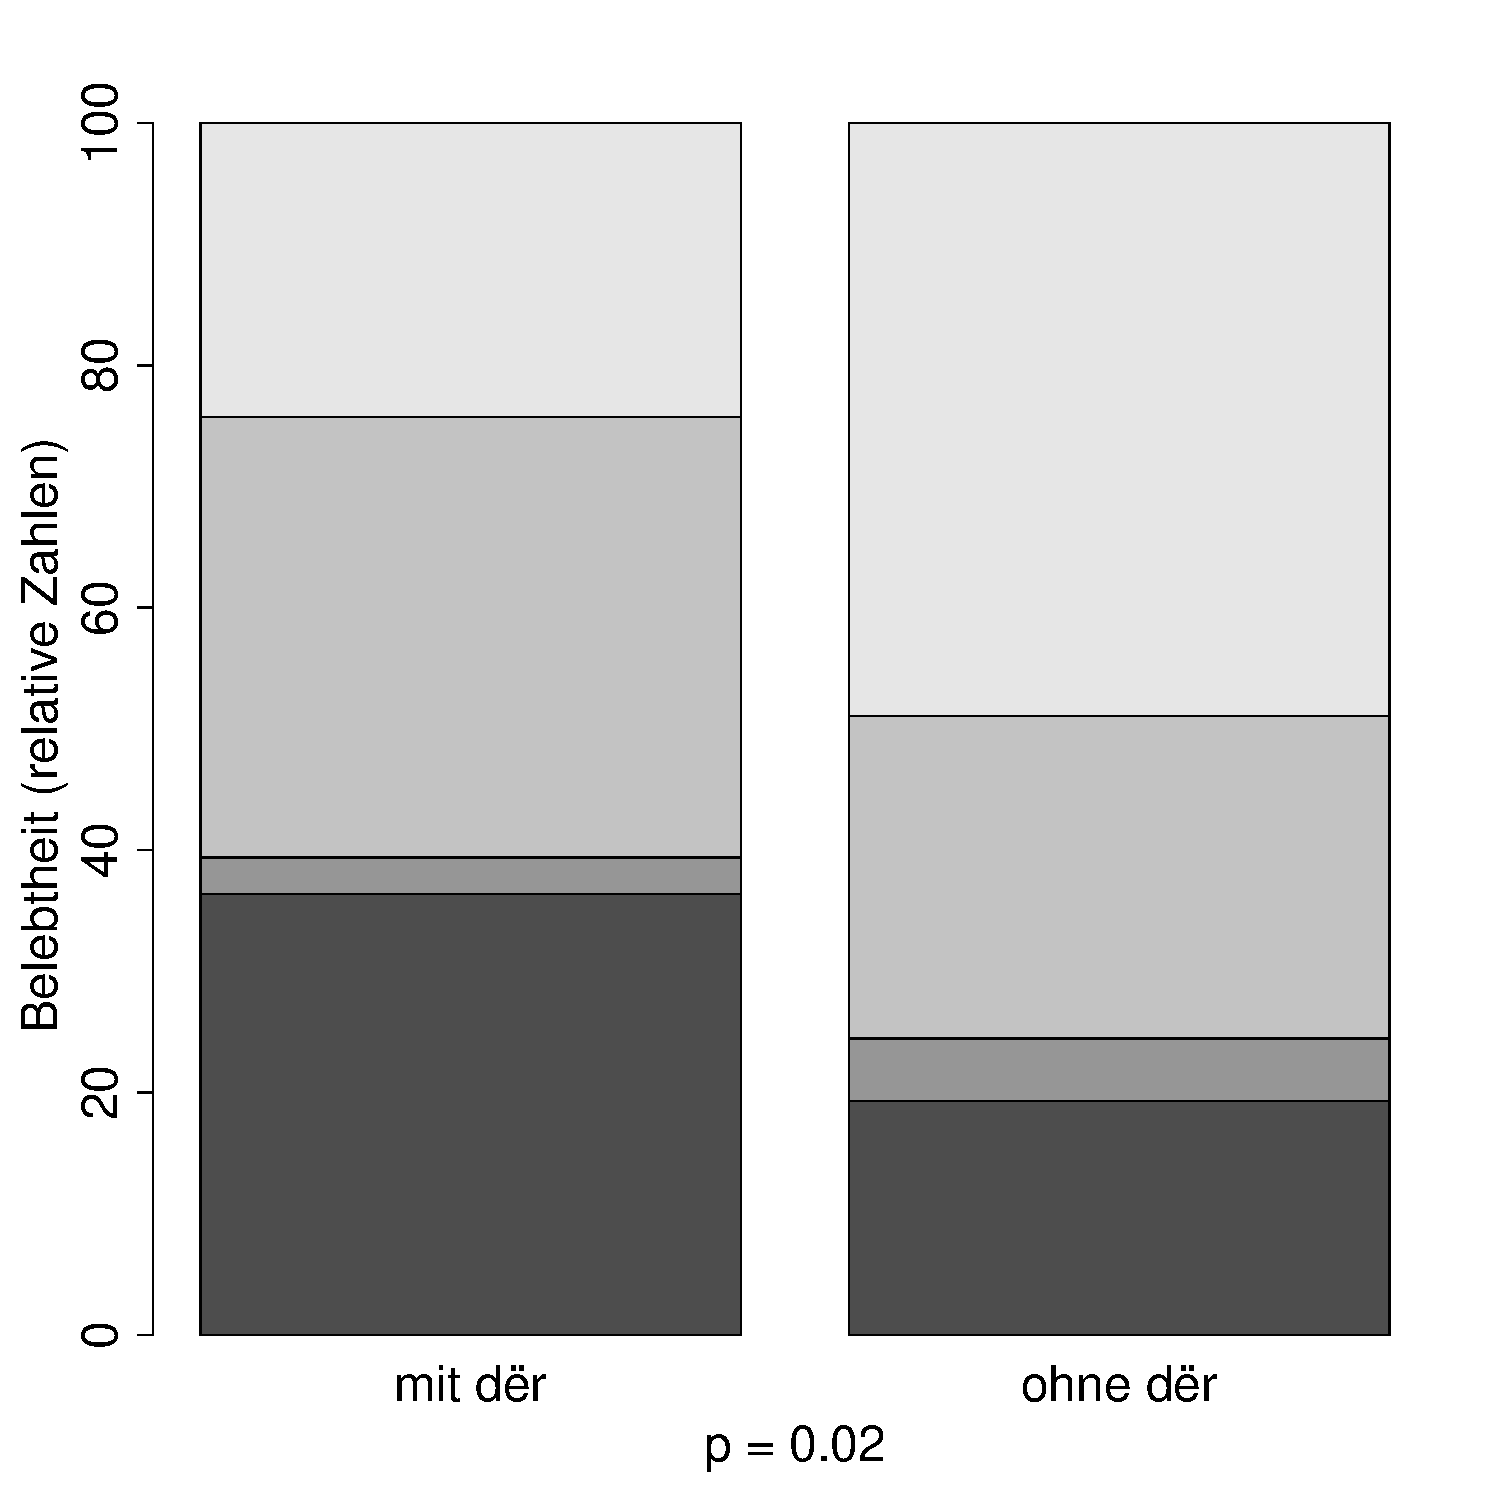
\includegraphics[height=.25\textheight]{generated/images/belebtheit-hapaxe-T}
\caption {Tatian}
\end{subfigure}%
\begin{subfigure}[b]{.5\linewidth}
  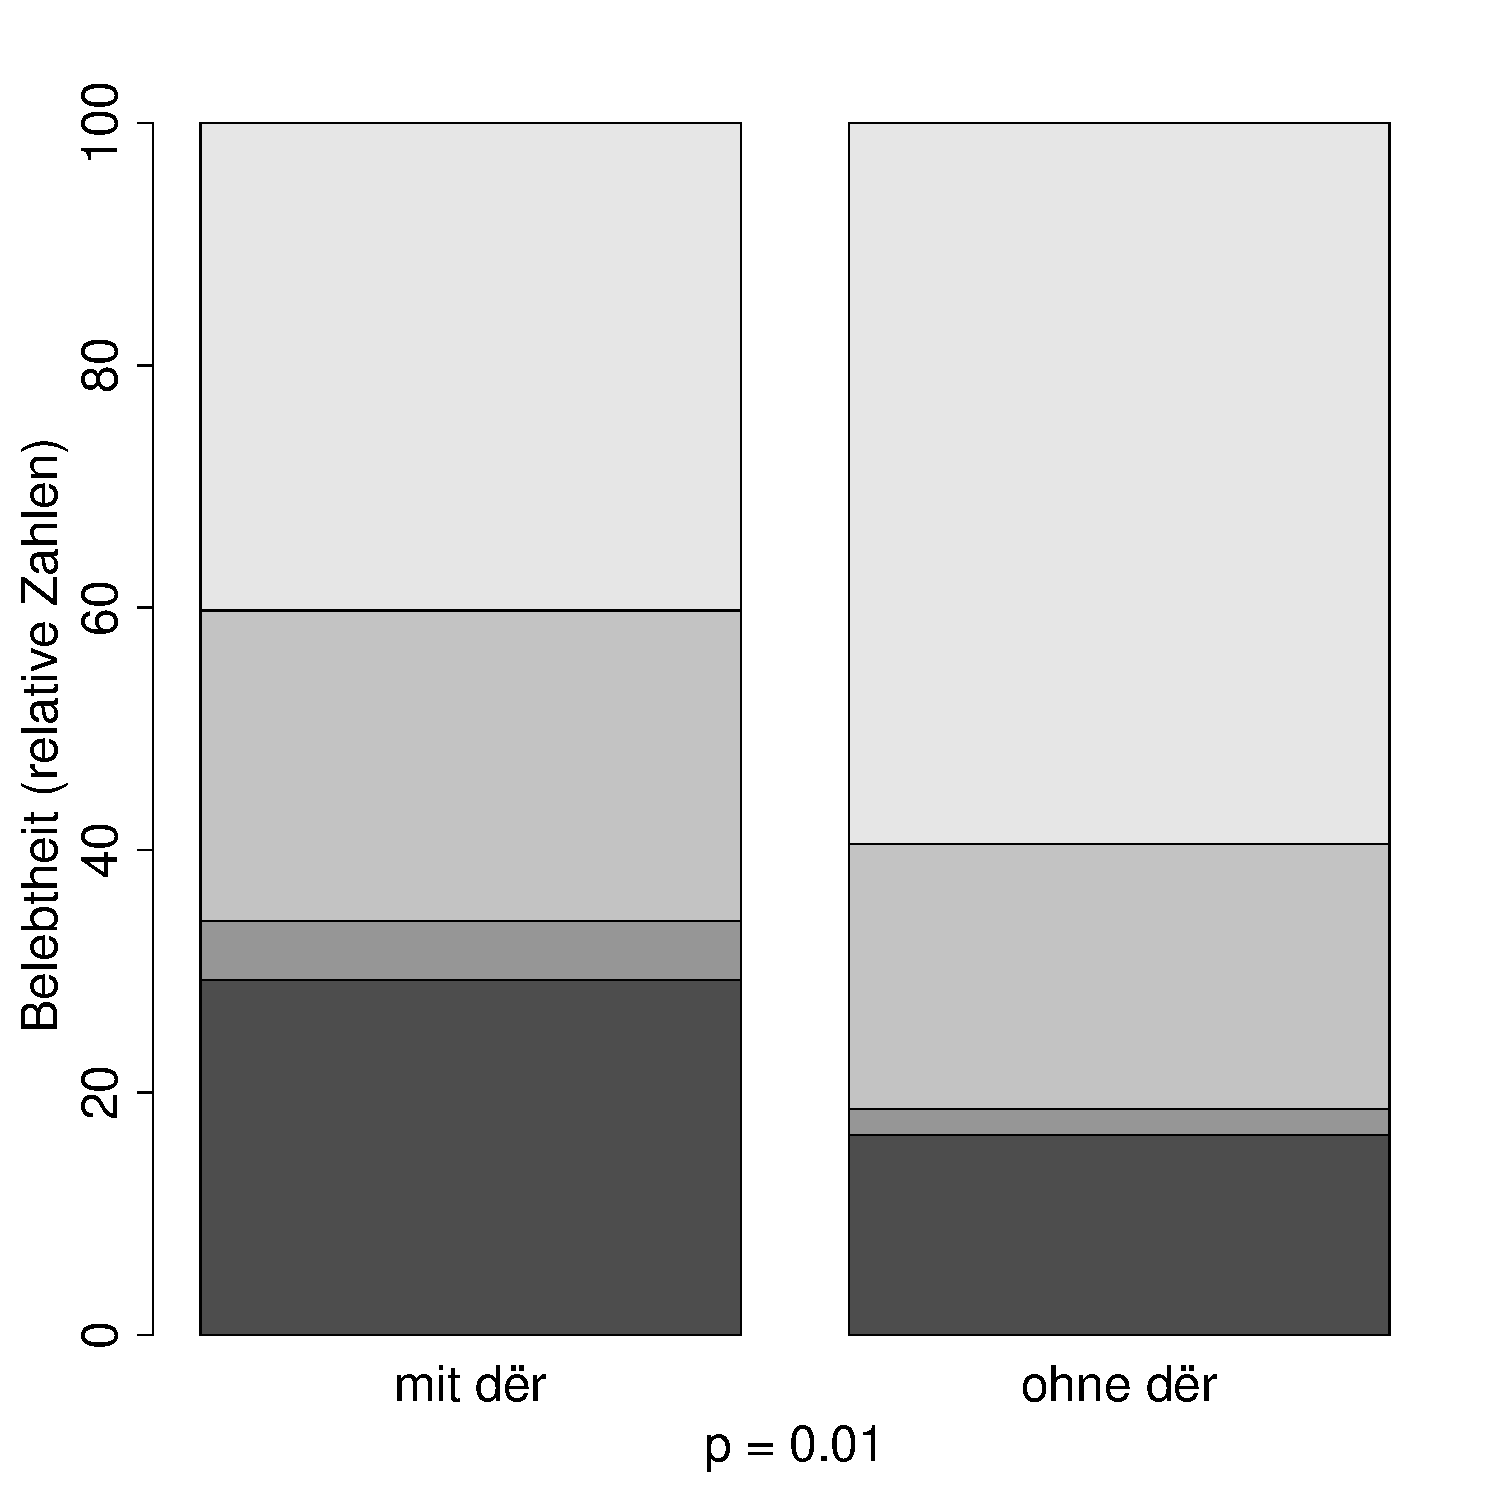
\includegraphics[height=.25\textheight]{generated/images/belebtheit-hapaxe-O}
\caption {Otfrid}
\end{subfigure}

\begin{subfigure}[b]{.5\linewidth}
  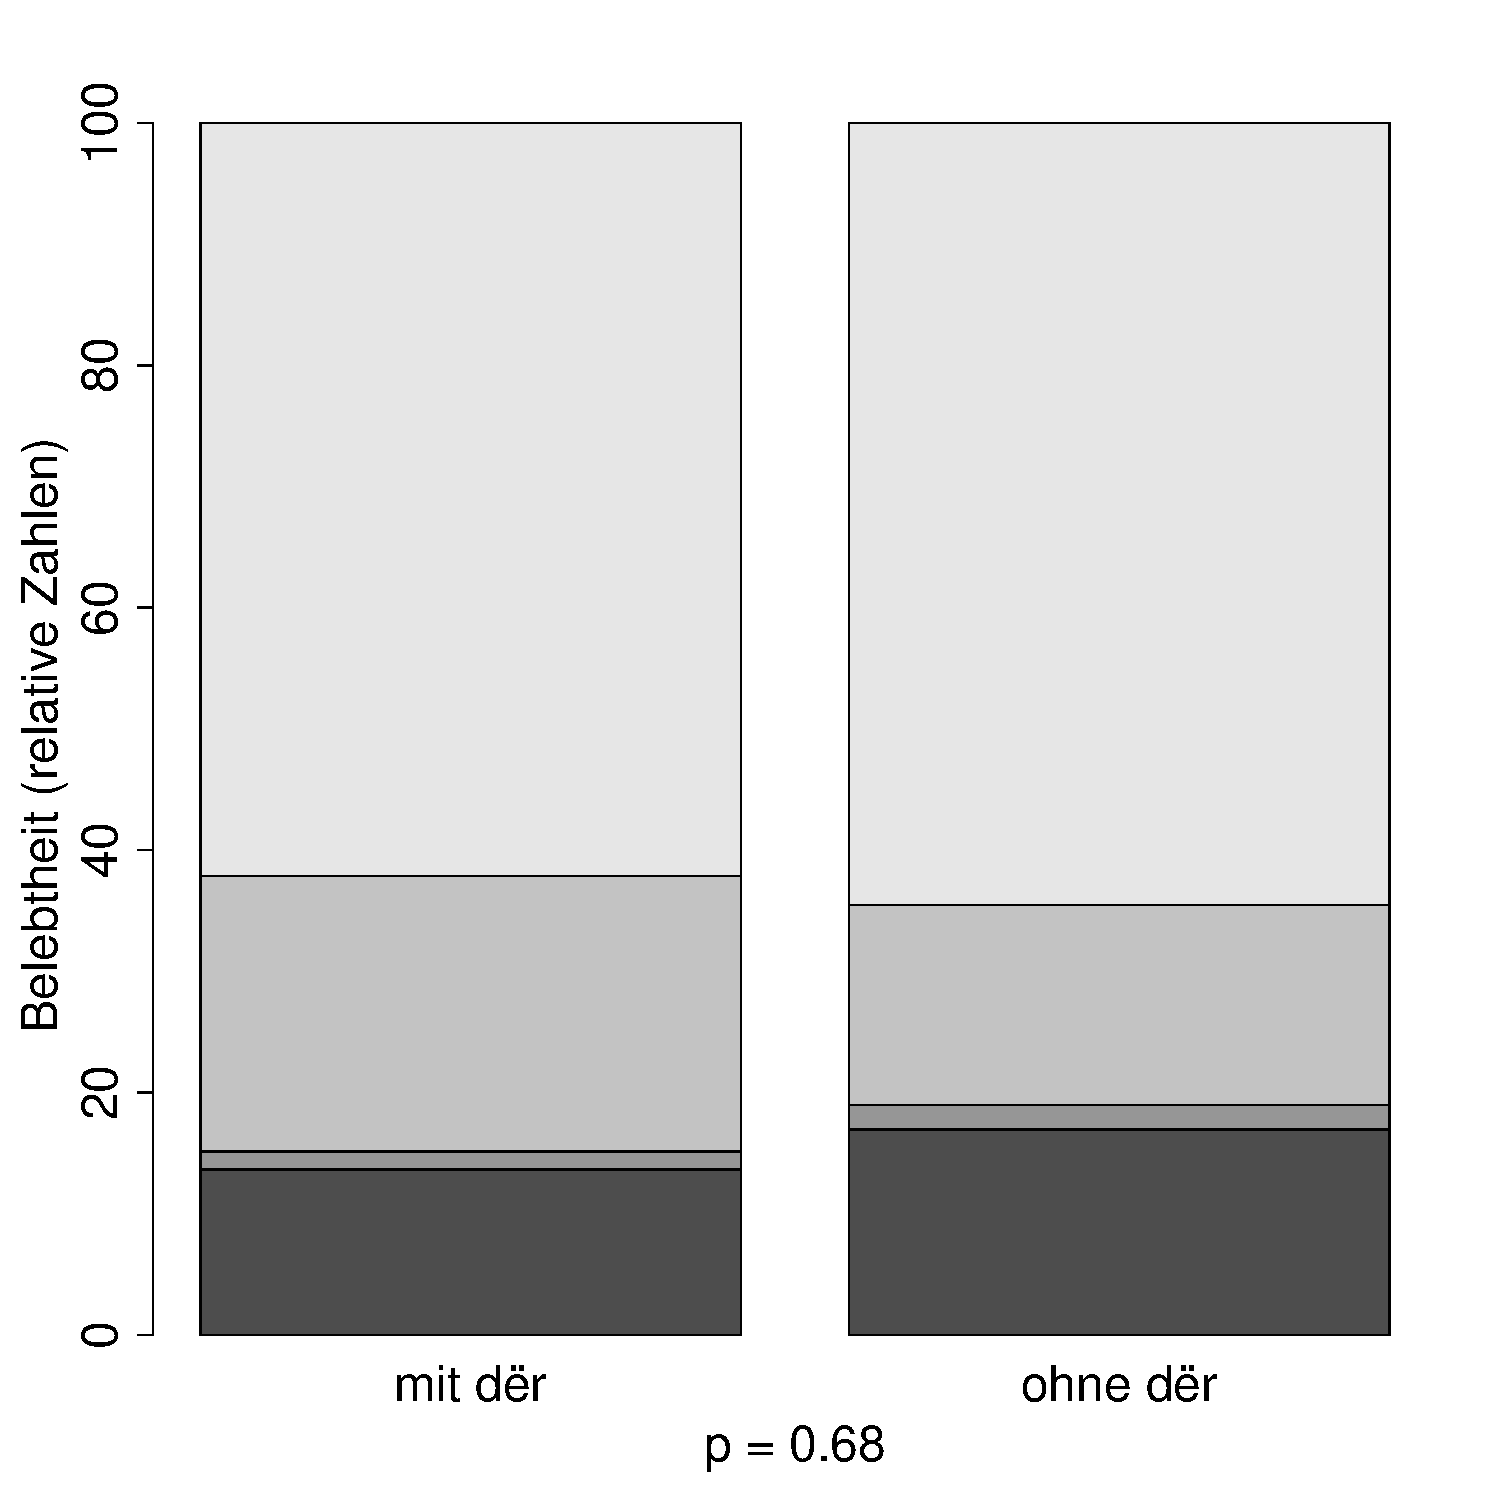
\includegraphics[height=.25\textheight]{generated/images/belebtheit-hapaxe-N}
\caption {Notker}
\end{subfigure}%
\begin{subfigure}[b]{.5\linewidth}
  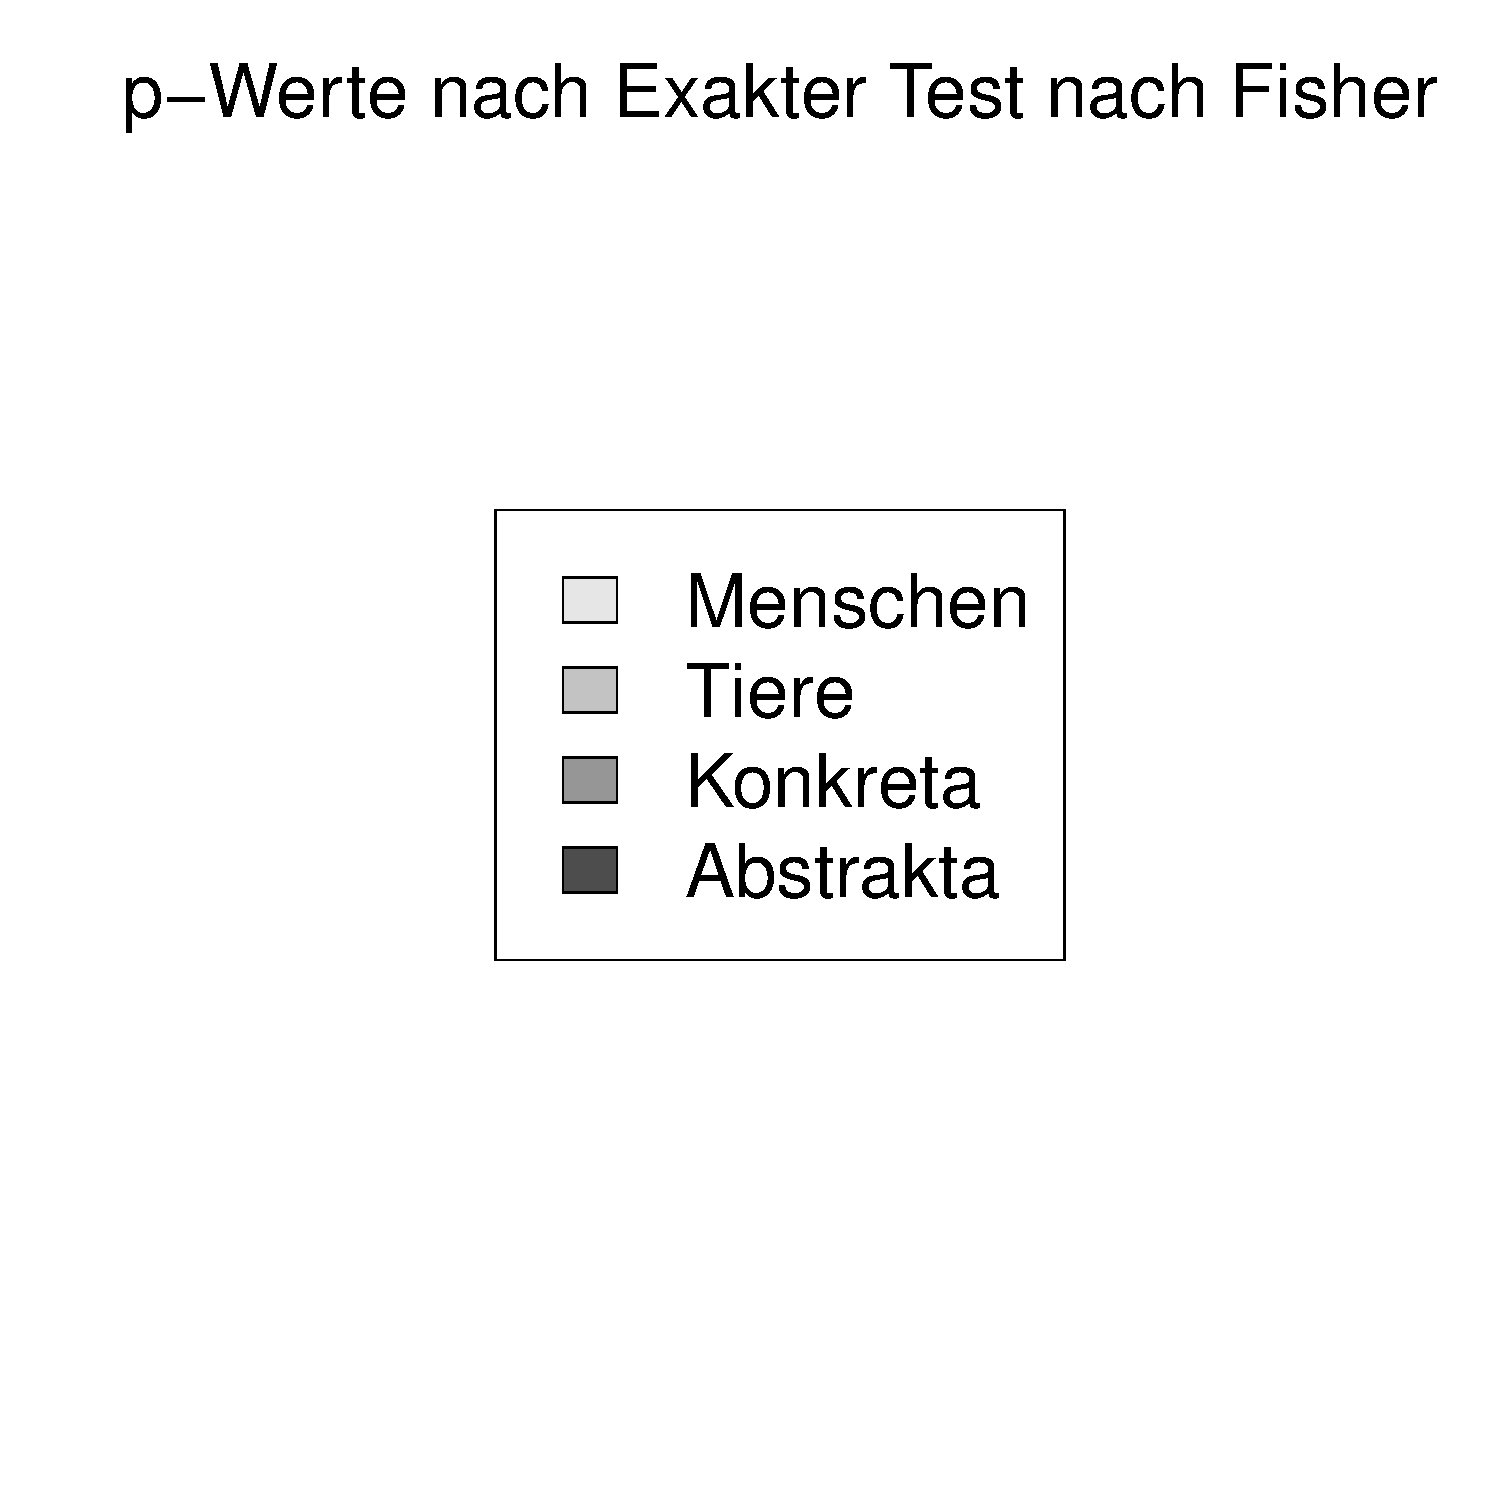
\includegraphics[height=.25\textheight]{generated/images/belebtheit-legende}
\end{subfigure}
\caption{Gebrauch von \object{dër} in Korrelation mit Belebtheit bei Hapax Legomena}\label{fig:bel-hapaxe}
\label{fig:residuals-bel-hapaxe}
\end{figure}

%\inputtable{generated/tables/bel.abs-hapaxe-I}{Gebrauch von \object{dër} in Korrelation mit Belebtheit bei Hapax Legomena; \\Isidor, absolute Zahlen}{tab:hapaxe-I}
%\inputtable{generated/tables/bel.abs-hapaxe-M}{Gebrauch von \object{dër} in Korrelation mit Belebtheit bei Hapax Legomena; \\Monseer Matthäus, absolute Zahlen}{tab:hapaxe-M}
%\inputtable{generated/tables/bel.abs-hapaxe-T}{Gebrauch von \object{dër} in Korrelation mit Belebtheit bei Hapax Legomena; \\Tatian, absolute Zahlen}{tab:hapaxe-T}
%\inputtable{generated/tables/bel.abs-hapaxe-O}{Gebrauch von \object{dër} in Korrelation mit Belebtheit bei Hapax Legomena; \\Otfrid, absolute Zahlen}{tab:hapaxe-O}
%\enlargethispage{1ex}
%\inputtable{generated/tables/bel.abs-hapaxe-N}{Gebrauch von \object{dër} in Korrelation mit Belebtheit bei Hapax Legomena; \\Notker, absolute Zahlen}{tab:hapaxe-N}



\begin{table}
\begin{tabular}{lrrrrrr}
  \lsptoprule
{Text} & {Struktur} & {Menschen} & {Tiere} & {Konkreta} & {Abstrakta} & {Summe} \\  
  \midrule
I & mit \object{dër} & 5 & 1 & 1 & 14 & 21 \\ 
 & ohne \object{dër} & 16 & 7 & 17 & 72 & 112 \\ 
 & Summe & 21 & 8 & 18 & 86 & 133 \\ 
   \midrule
M & mit \object{dër} & 6 & 0 & 5 & 6 & 17 \\ 
 & ohne \object{dër} & 15 & 5 & 27 & 51 & 98 \\ 
 & Summe & 21 & 5 & 32 & 57 & 115 \\ 
  \midrule
T & mit \object{dër} & 12 & 1 & 12 & 8 & 33 \\ 
 & ohne \object{dër} & 45 & 12 & 62 & 114 & 233 \\ 
 & Summe & 57 & 13 & 74 & 122 & 266 \\ 
  \midrule
O & mit \object{dër} & 24 & 4 & 21 & 33 & 82 \\ 
 & ohne \object{dër} & 46 & 6 & 61 & 166 & 279 \\ 
 & Summe & 70 & 10 & 82 & 199 & 361 \\ 
  \midrule
N & mit \object{dër} & 9 & 1 & 15 & 41 & 66 \\ 
 & ohne \object{dër} & 42 & 5 & 41 & 160 & 248 \\ 
 & Summe & 51 & 6 & 56 & 201 & 314 \\ 
   \lspbottomrule
\end{tabular}
\caption{Gebrauch von \object{dër} in Korrelation mit \isi{Belebtheit} bei Hapax Legomena (absolute Zahlen)}
\label{tab:hapaxe}
\end{table}

% Residuals Hapaxe

\begin{figure}
\begin{subfigure}[b]{.5\linewidth}
  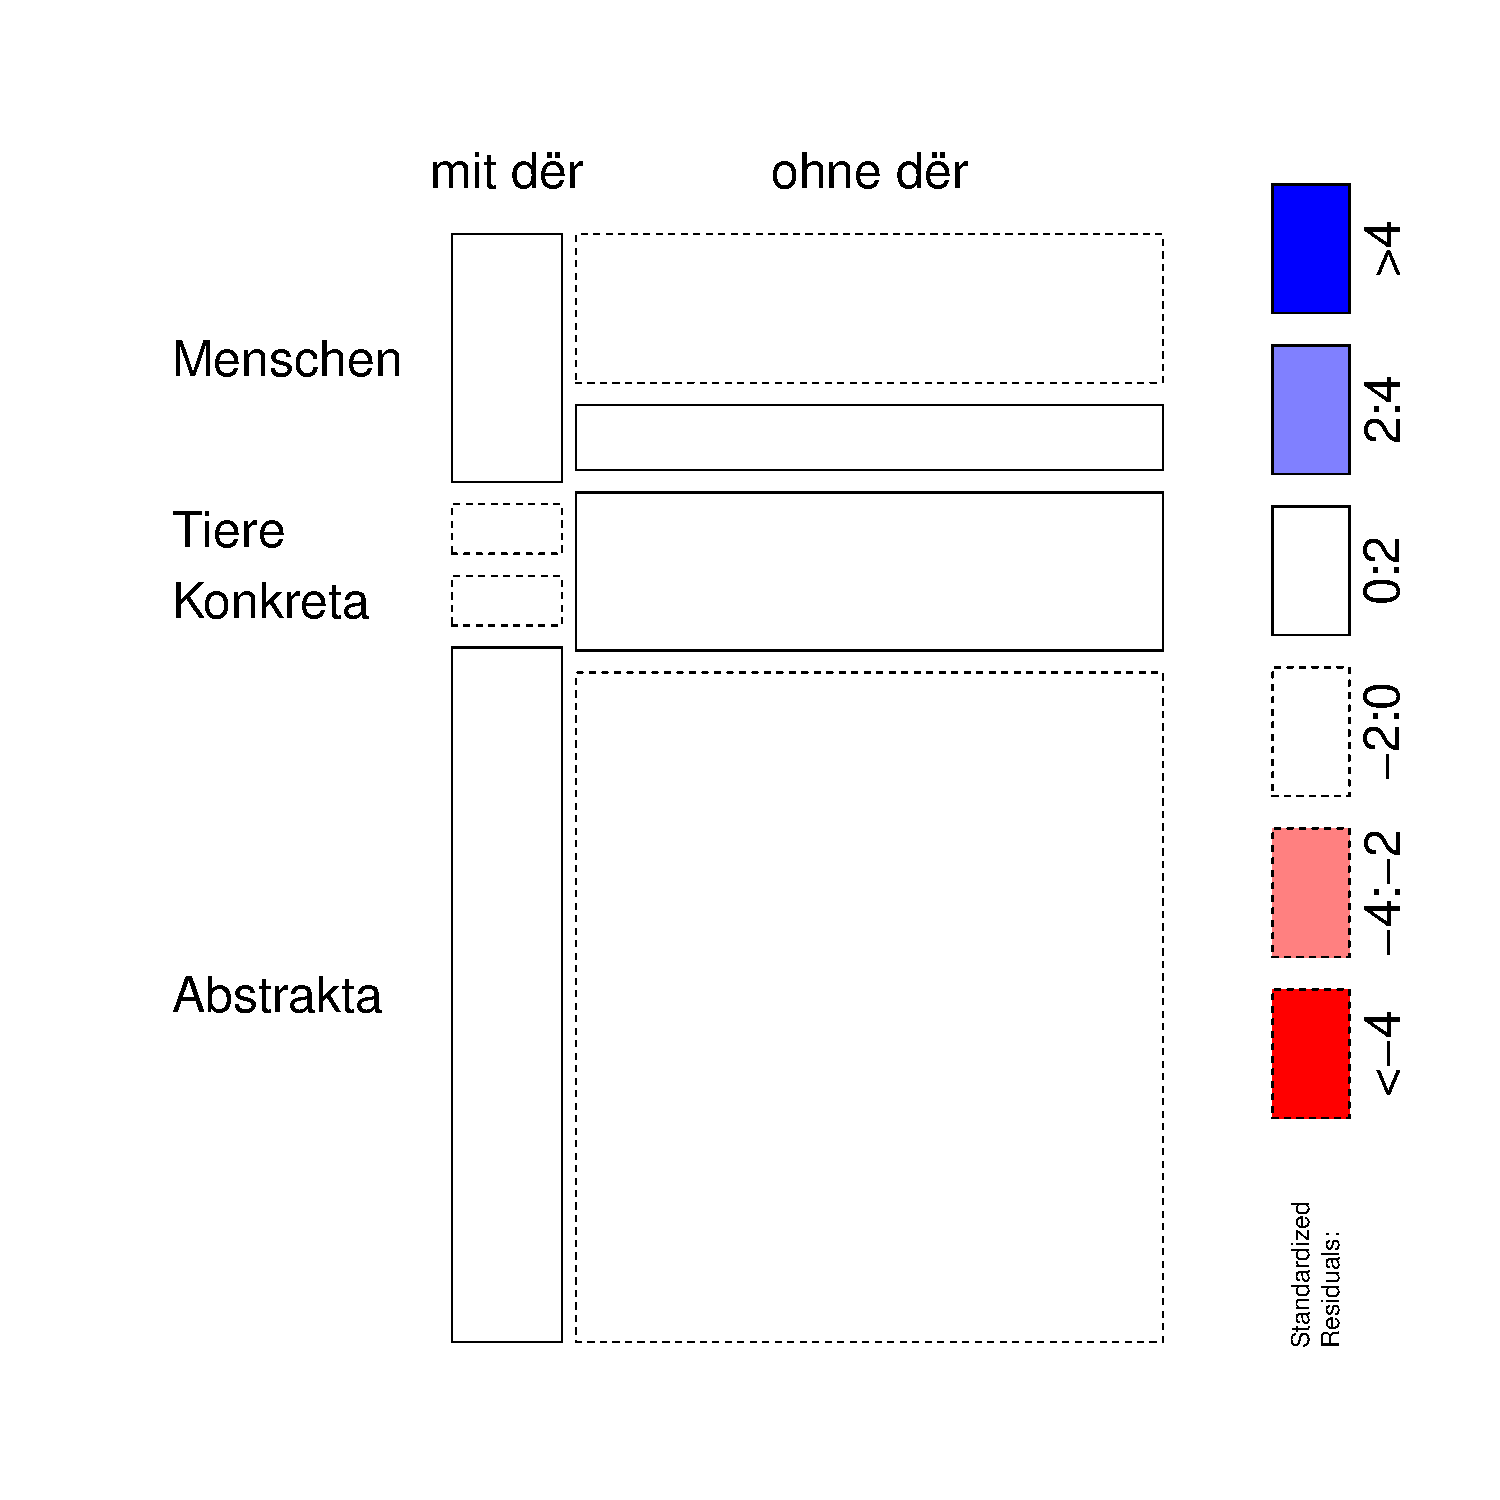
\includegraphics[height=.25\textheight]{generated/images/bel-hapaxe-residuals-I}
\caption {Isidor}
\end{subfigure}%
\begin{subfigure}[b]{.5\linewidth}
  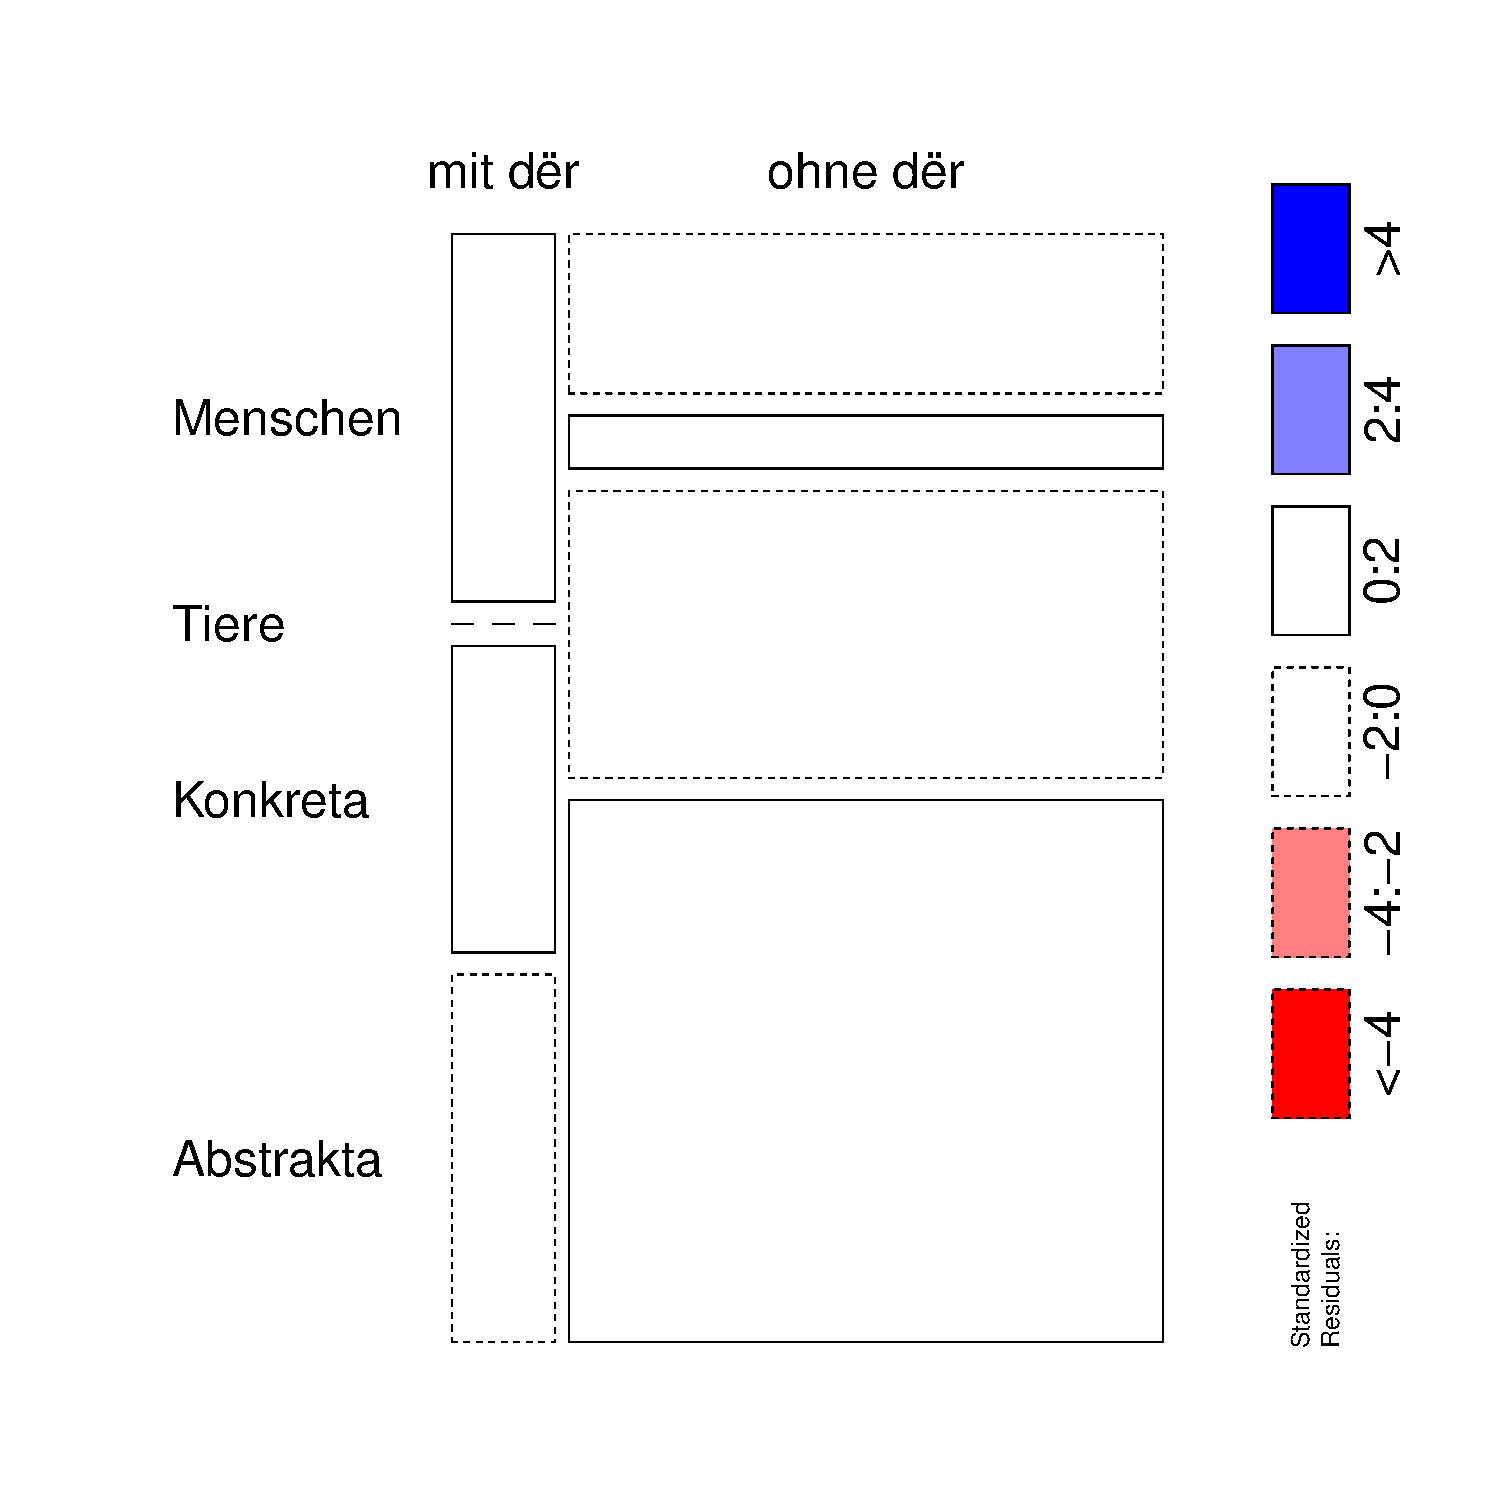
\includegraphics[height=.25\textheight]{generated/images/bel-hapaxe-residuals-M}
\caption {Monseer Matthäus}
\end{subfigure}

\begin{subfigure}[b]{.5\linewidth}
  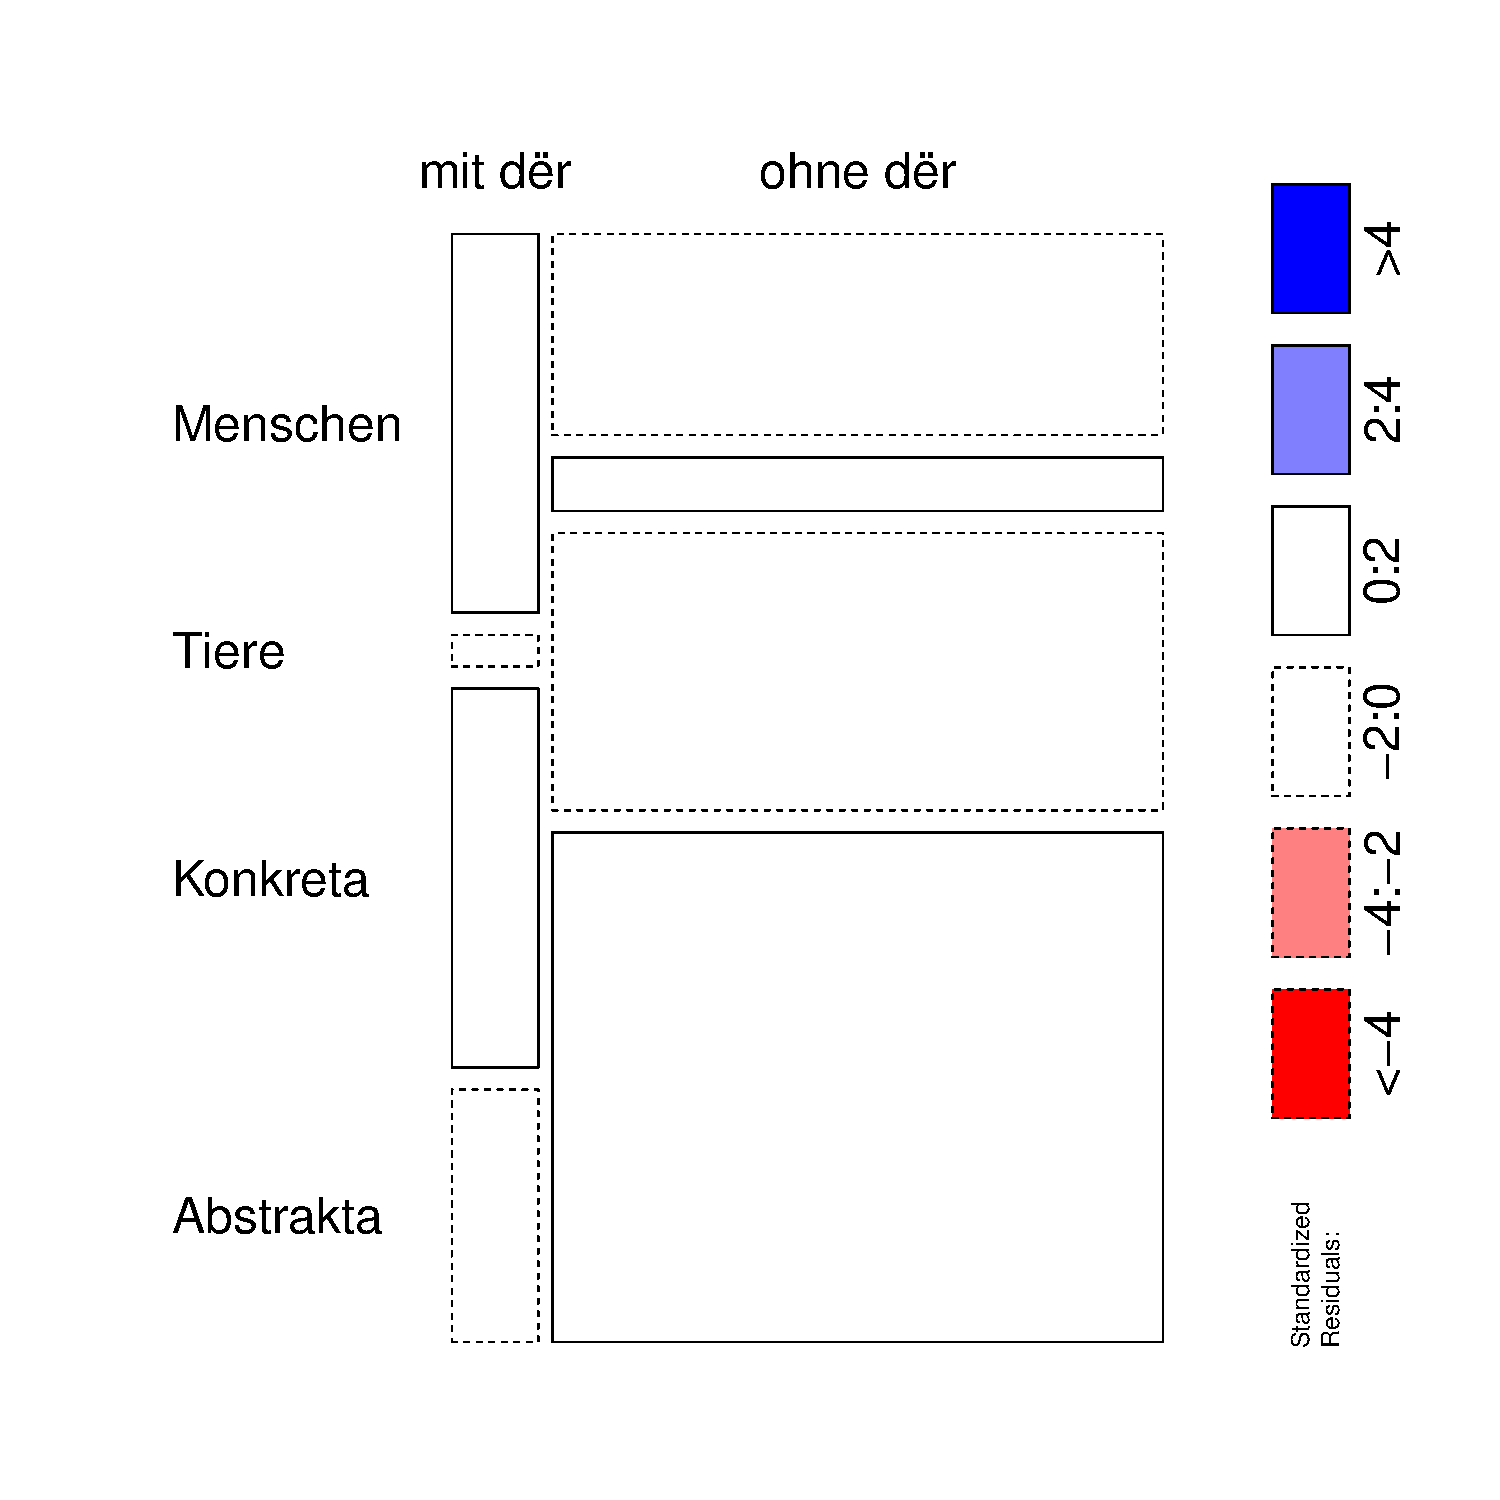
\includegraphics[height=.25\textheight]{generated/images/bel-hapaxe-residuals-T}
\caption {Tatian}
\end{subfigure}%
\begin{subfigure}[b]{.5\linewidth}
  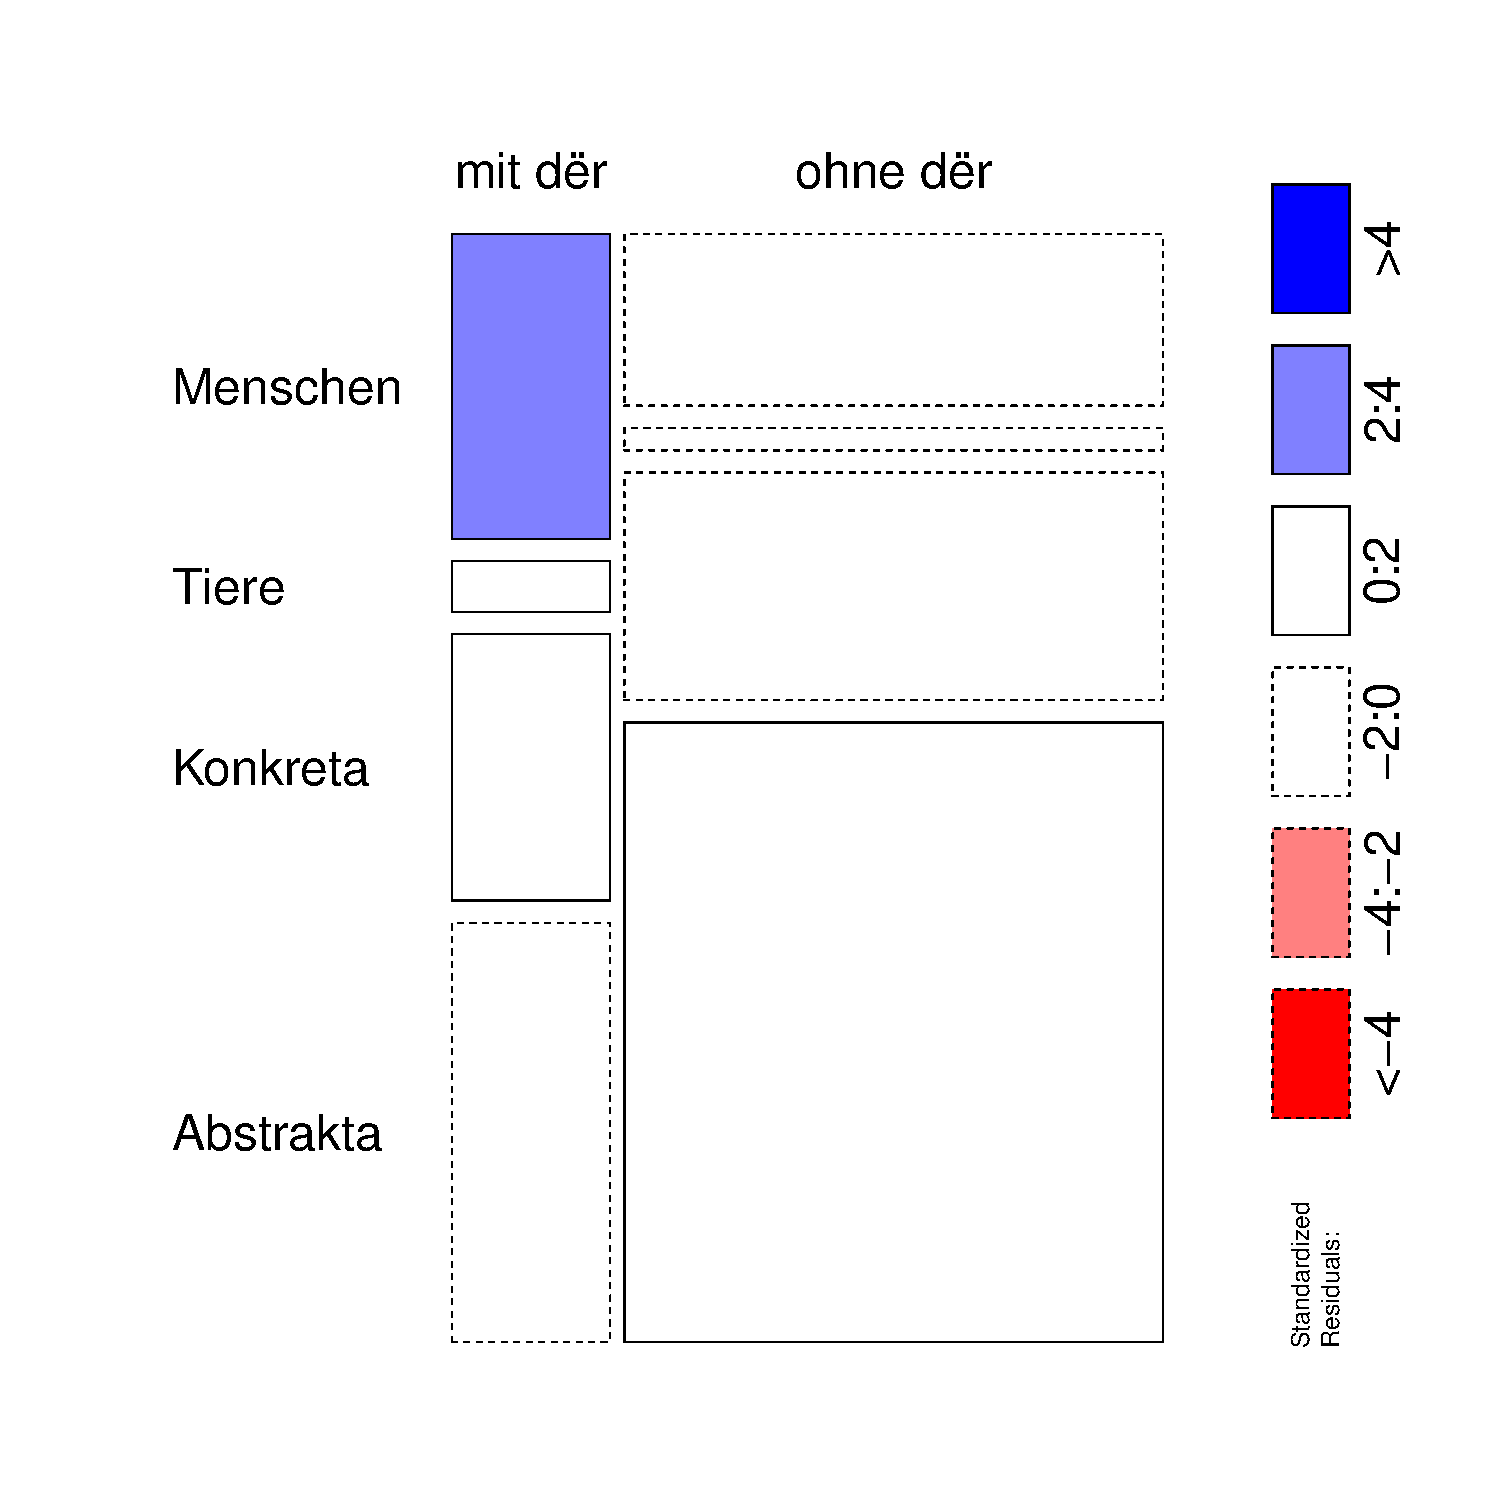
\includegraphics[height=.25\textheight]{generated/images/bel-hapaxe-residuals-O}
\caption {Otfrid}
\end{subfigure}

\begin{subfigure}[b]{.5\linewidth}
  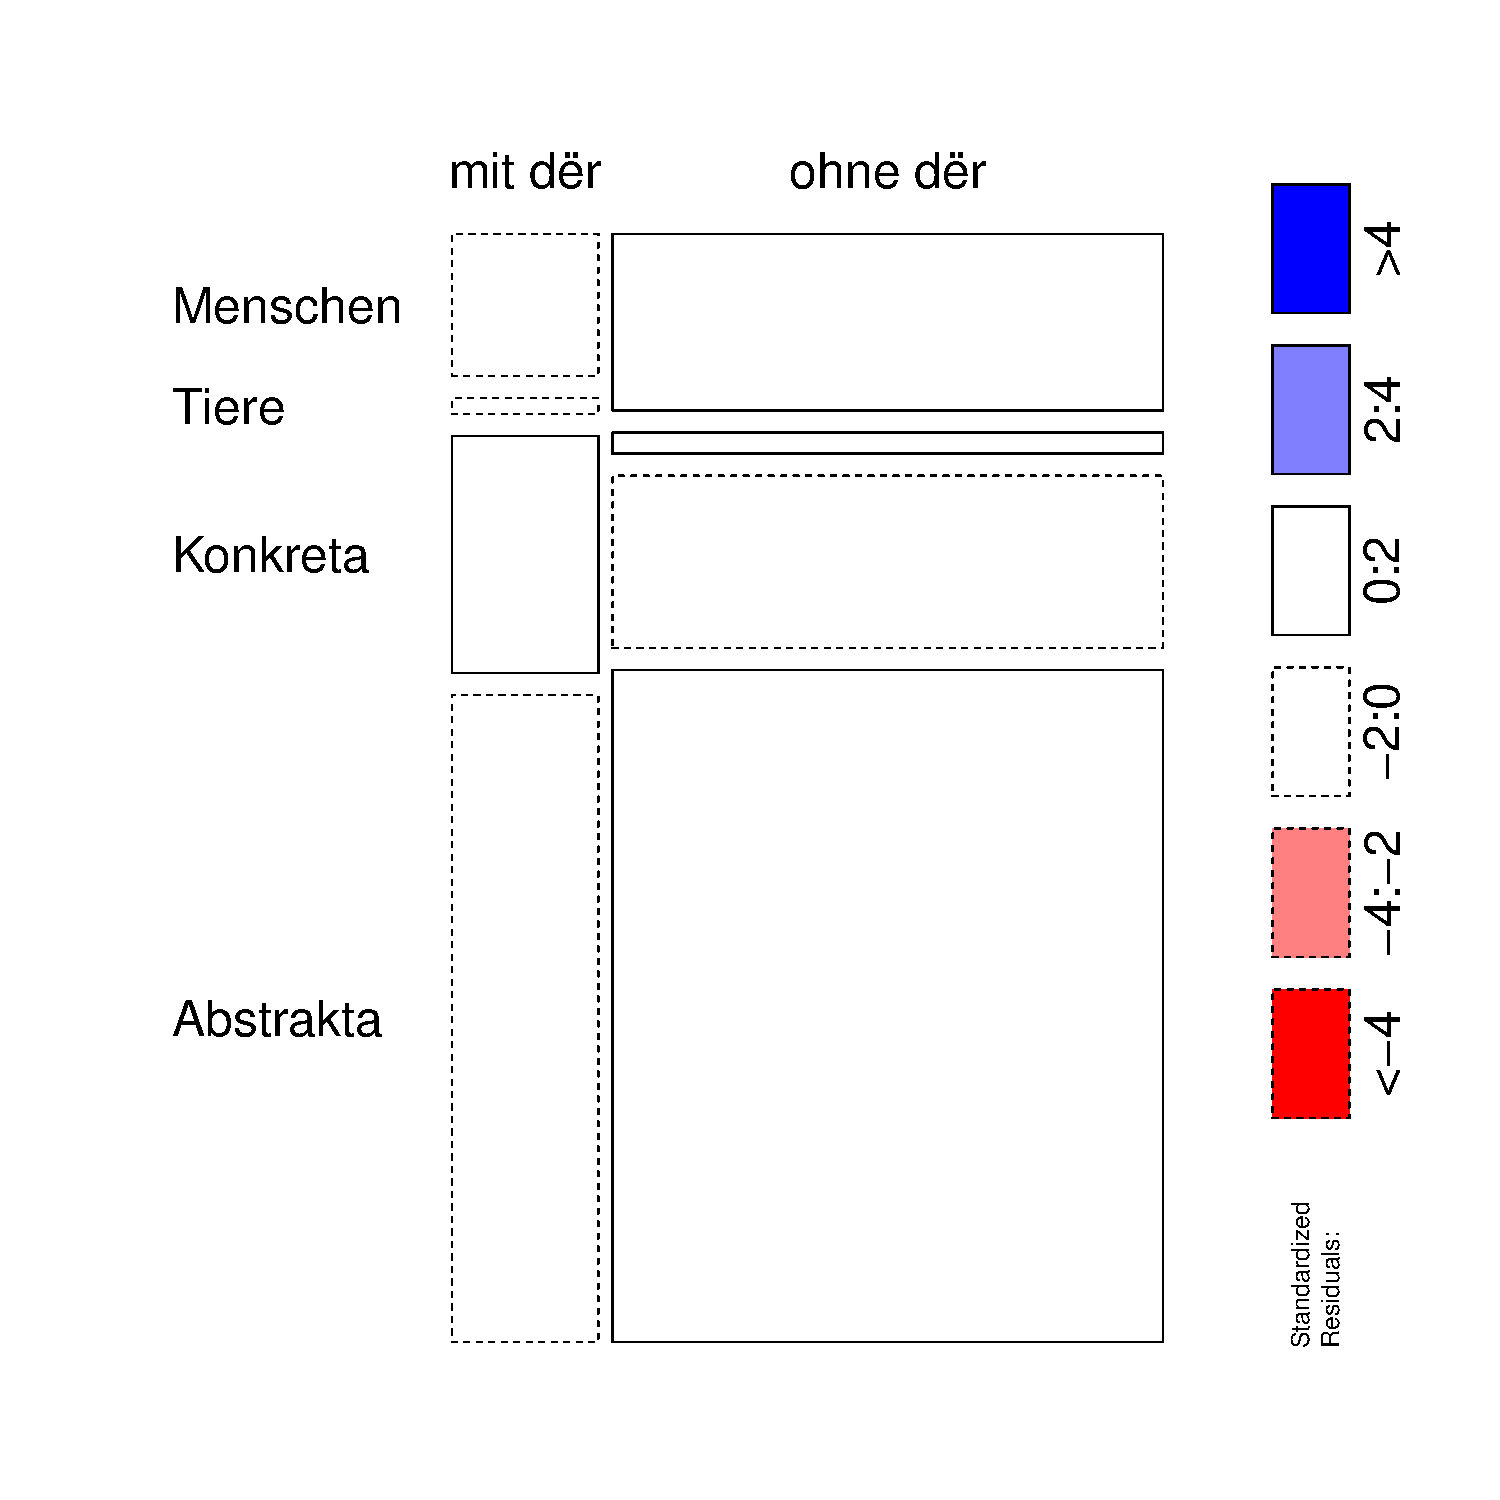
\includegraphics[height=.25\textheight]{generated/images/bel-hapaxe-residuals-N}
\caption {Notker}
\end{subfigure}
\caption{Einfluss von \isi{Belebtheit} auf \object{dër}-Gebrauch bei Hapax Legomena (Residuen)}
\label{fig:bel-hapaxe-residuals}
\end{figure}

%\subsubsection{Subkategorien Konkreta: Körperteile und Orte}
Eine weitere wichtige Gruppe, die im Rahmen der Belebtheitsannotation \is{Belebtheit}\is{Annotation}untersucht wurde, sind Körperteile. Sie sind auf der Belebtheitsskala \is{Belebtheitshierarchie} höher zu verorten als andere \is{Konkretum} Konkreta, da sie nicht veräußerbar sind und vom Menschen stärker kontrolliert werden können. Außerdem weisen sie in der Regel eine eindeutige Referenz \is{Referentialität} auf, so dass sie semantische Definita \is{Semantische Definita} repräsentieren (s.  Abschnitt~\ref{sec:pragsem}). Deshalb kann der emergierende Artikel erst nach dem Verlust seiner demonstrativen Funktion in die Domäne der Körperteile eindringen (vgl. hierzu auch Abschnitt~\ref{sec:schema}). Zudem existiert mit dem Possessivartikel \is{Possessivum} bereits ein \isi{Determinierer}, der den pränominalen Slot besetzt, und Besitzverhältnisse bzw. die Zugehörigkeit von Körperteilen zum Körper anzeigen kann. Es ist deswegen zu erwarten, dass Belege mit \object{dër} hier erst in den späteren Texten zu finden sind.\largerpage[-2]

Wie an den Häufigkeiten in Abbildung~\ref{fig:bel-koerper} abzulesen ist, zeichnet sich in Otfrids Evangelienbuch und Notkers Boethius eine  Kontextexpansion \is{Expansion} von \object{dër} auf den Bereich der Körperteile ab. 
In den drei frühsten Texten kommen nur vereinzelt Phrasen mit \object{dër}\,+\,Körperteil vor: Im Isidor ist es nur ein einzelner Belege (\object{lihhamo}). Im Monseer Matthäus ist der einzige determinierte Beleg \object{bluot}. Beide Referenten sind also keine typischen Vertreter der Kategorien \hervor{Körperteile}. Im Tatian finden sich darüber hinaus auch bei typischen Körperteilen wie \object{hërza}, \object{hand},  \object{mund} und \object{ouga} einzelne Belege mit \object{dër}. Bei Otfrid und Notker machen die determinierten Fälle immerhin knapp ein Drittel der Gesamtbelege aus. Bei Otfrid sind es die Lemmata \is{Lemma} \object{brust},  \object{lihhamo},  \object{ouga} und \object{houbit}, die herausstechen, da diese mit zweistelligen Tokenwerten vertreten sind und in jedem dritten Gebrauch determiniert werden. Alle anderen Lemmata \is{Lemma} für Körperteile bleiben in der Mehrzahl undeterminiert. Bei Notker kommt nur \object{ouga} über eine Tokenzahl von zehn -- in 4 von 14 Fällen steht es mit \object{dër}.

\begin{figure}
\begin{subfigure}[c]{.75\linewidth}
  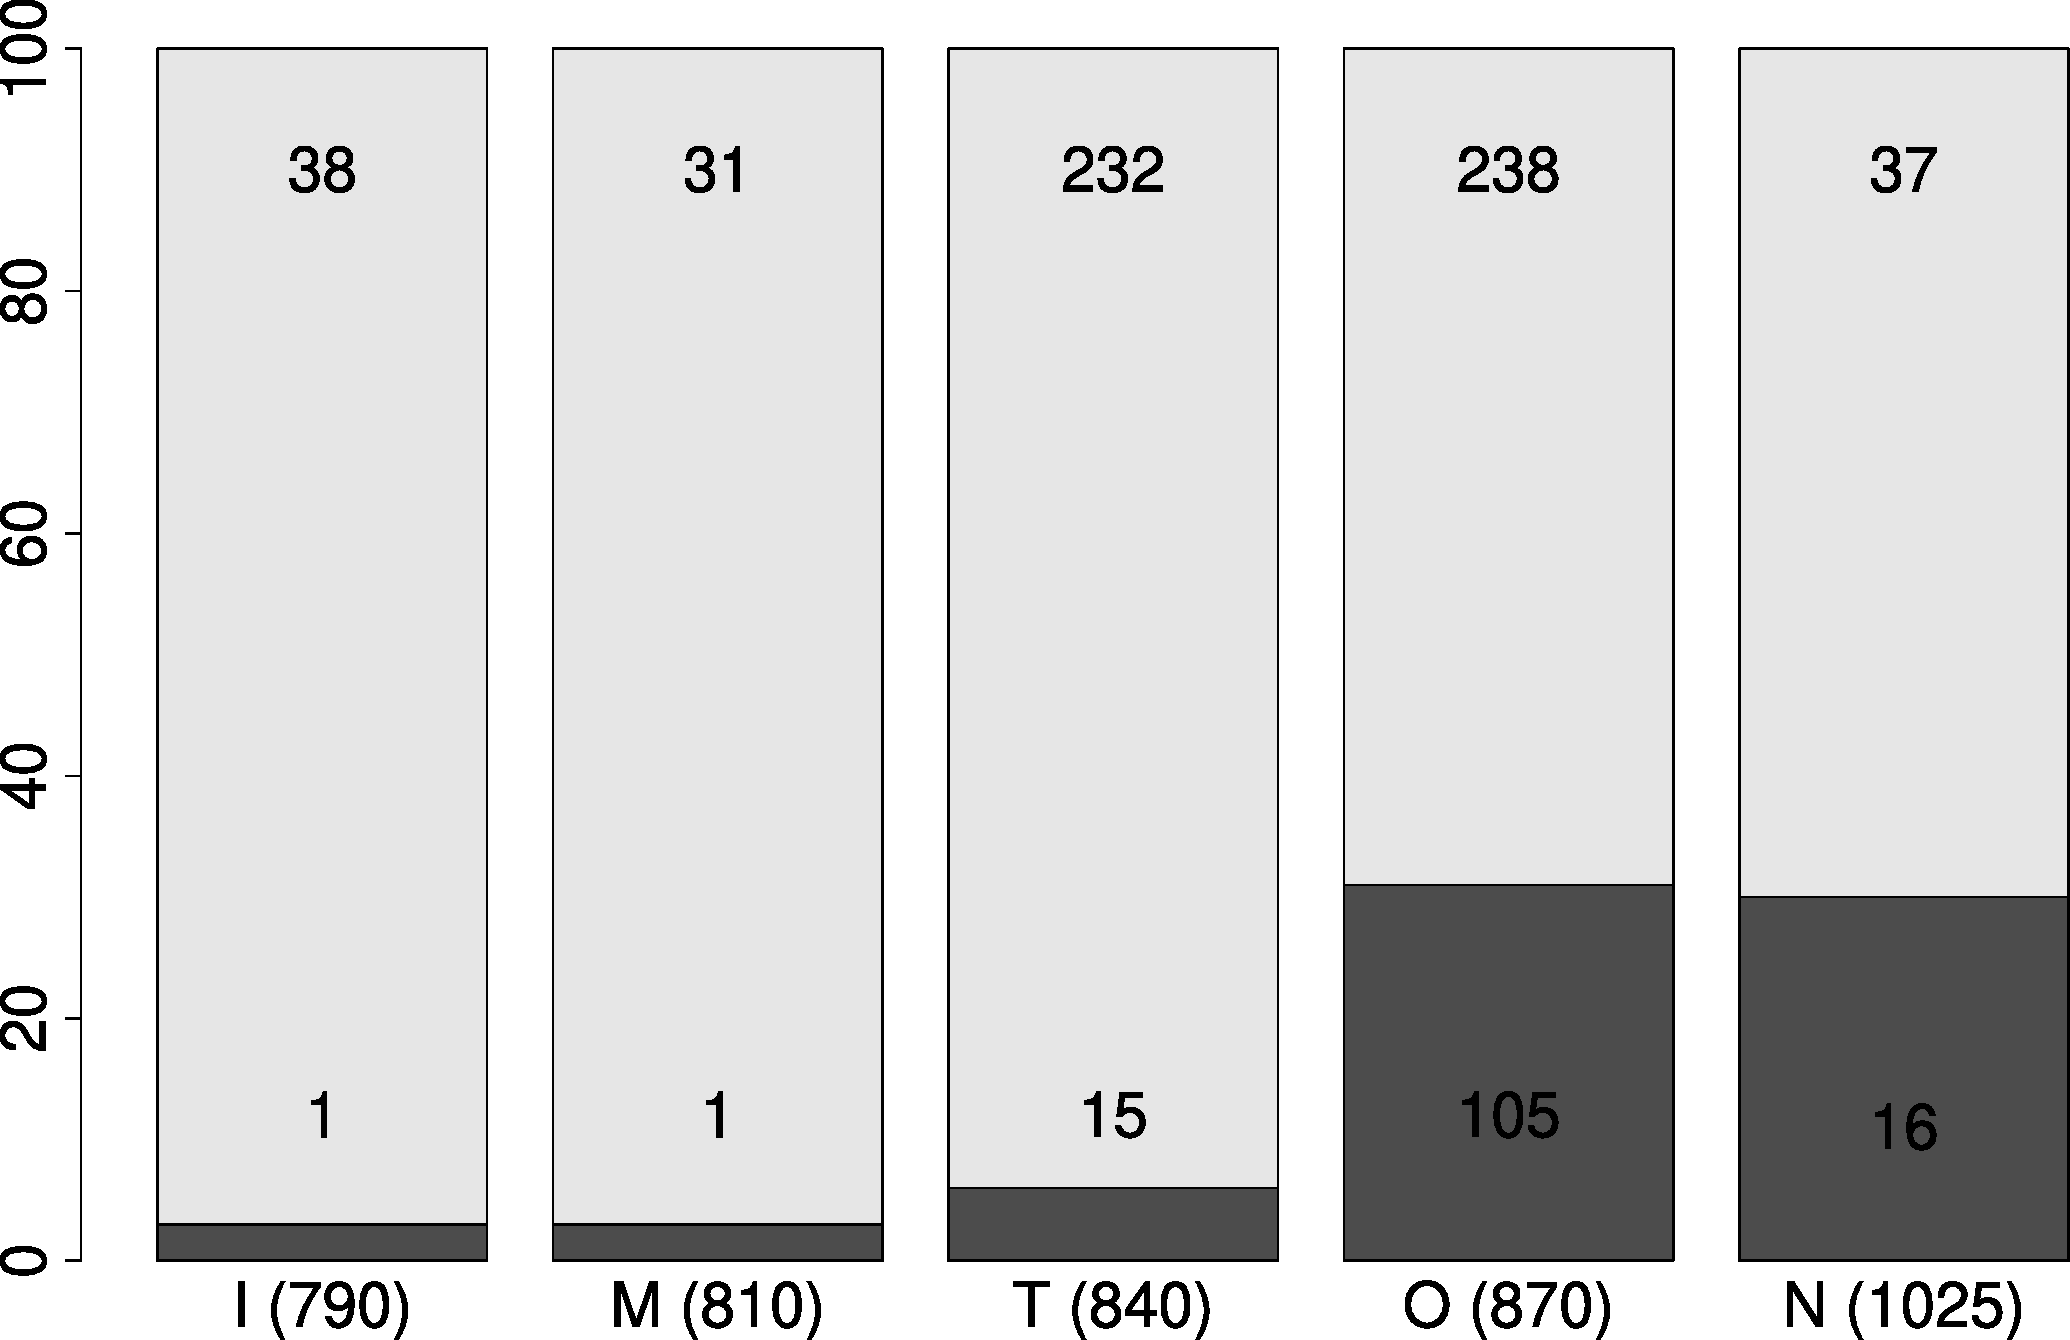
\includegraphics[width=\linewidth]{generated/images/koerper}
\end{subfigure}%
\begin{subfigure}[c]{.2\linewidth}
  
\includegraphics[width=.85\linewidth]{generated/images/ort-legende}
\end{subfigure}

\caption{Gebrauch von \object{dër} bei Bezeichnungen für Körperteile}
\label{fig:bel-koerper}
\end{figure}

Eine weitere Subkategorie der Konkreta \is{Konkretum} sind Orte. Sie wurden separat annotiert, weil sie sich als typische Kandidaten für adverbiale \is{Adverbial} und damit nicht-referentielle Phrasen möglicherweise anders verhalten als die restlichen \is{Konkretum} Konkreta. Der Vergleich von Appellativa \is{Gattungsname} mit und ohne \object{dër} bei dieser Gruppe ist für die einzelnen Texte in Abbildung~\ref{fig:bel:orte} zu sehen. In allen Texten sind Phrasen von \object{dër}\,+\,Ortsangabe zu finden. In den drei ältesten Denkmälern (Isidor, Monseer Matthäus und Tatian) machen diese gut ein Viertel der Belege aus, bei Otfrid sind es fast die Hälfte und auch Notker kommt annähernd auf 25\%. Die Durchsicht der Belege ergibt, dass Orte sowohl auf konkrete Referenten verweisen (z.B. \object{hus} oder \object{burg}) als auch nicht-referentiell auftreten, etwa in der Funktion von adverbialen \is{Adverbial} Angaben in Form von PPs (vgl. auch Abschnitt \ref{sec:ergeb-partizipanten}).
Allein die Tatsache, dass ein Referent auf einen Ort verweist, reicht also nicht aus, um Rückschlüsse auf den Gebrauch von \object{dër} zu ziehen. Faktoren wie Phrasentyp und semantische Rolle \is{Semantische Rolle} müssten in zukünftigen Untersuchungen einbezogen werden.  

\begin{figure}
\begin{subfigure}[c]{.75\linewidth}
  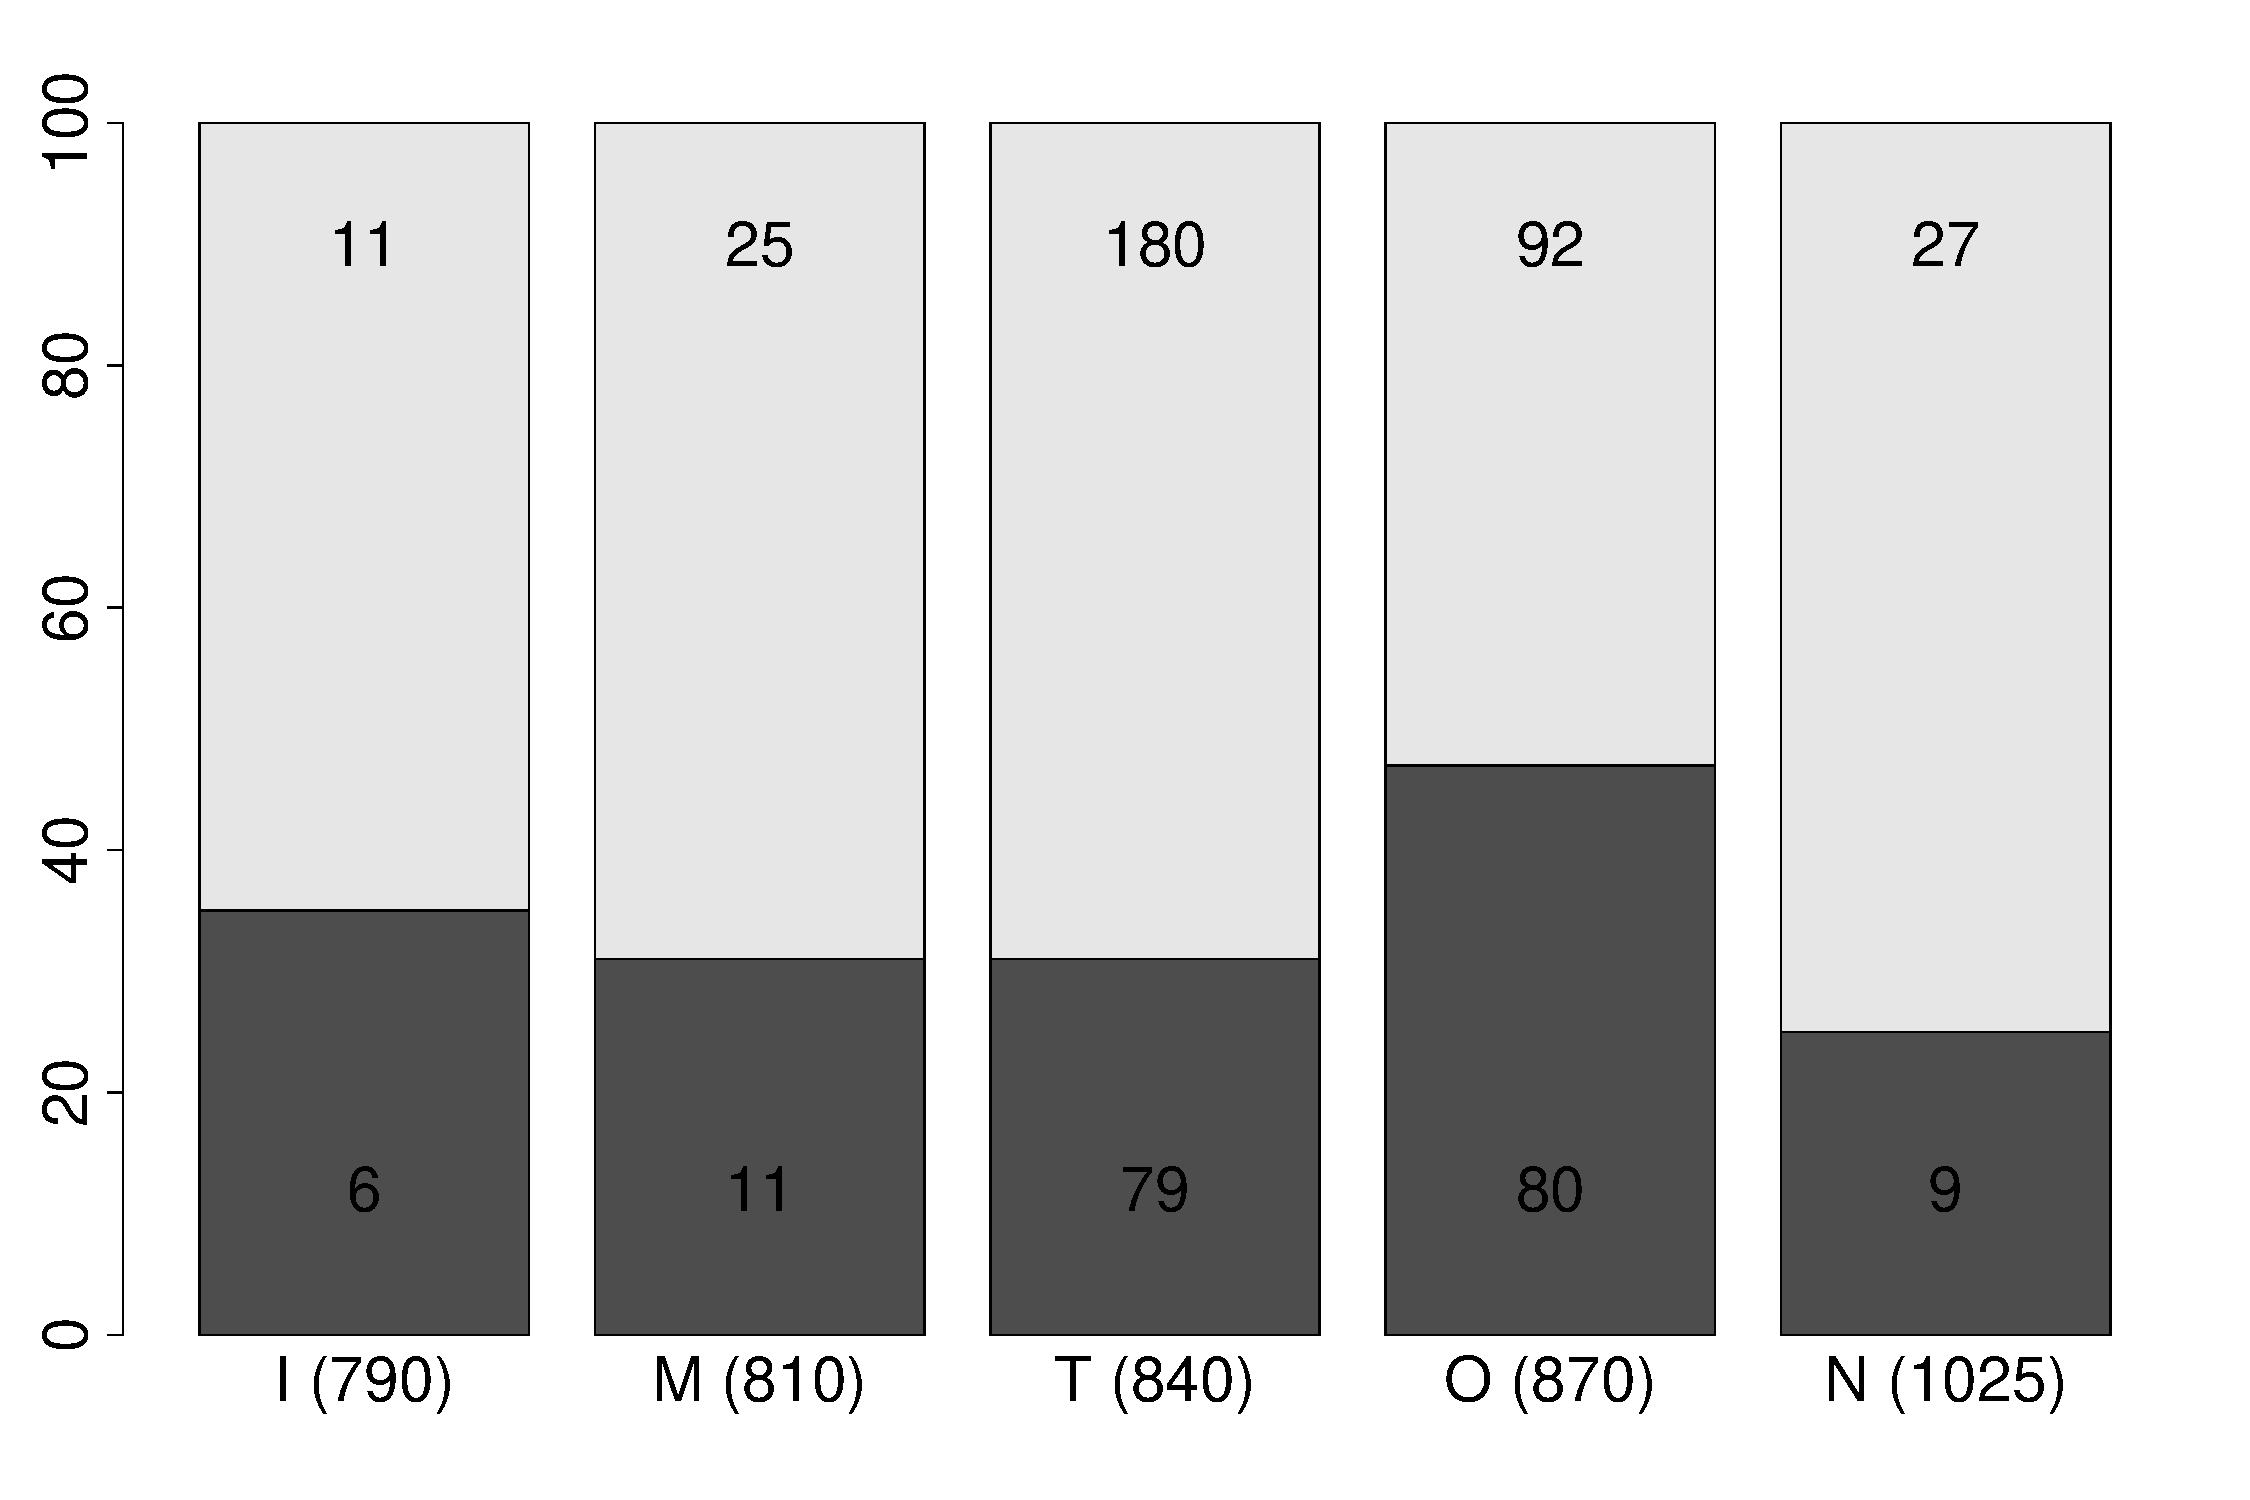
\includegraphics[width=\linewidth]{generated/images/ort}
\end{subfigure}%
\begin{subfigure}[c]{.2\linewidth}
  
\includegraphics[width=.85\linewidth]{generated/images/ort-legende}
\end{subfigure}
\caption{Gebrauch von \object{dër} bei Ortsbezeichnungen}
  \label{fig:bel:orte}
\end{figure} 

% \begin{figure}
% \begin{subfigure}[b]{.5\linewidth}
%   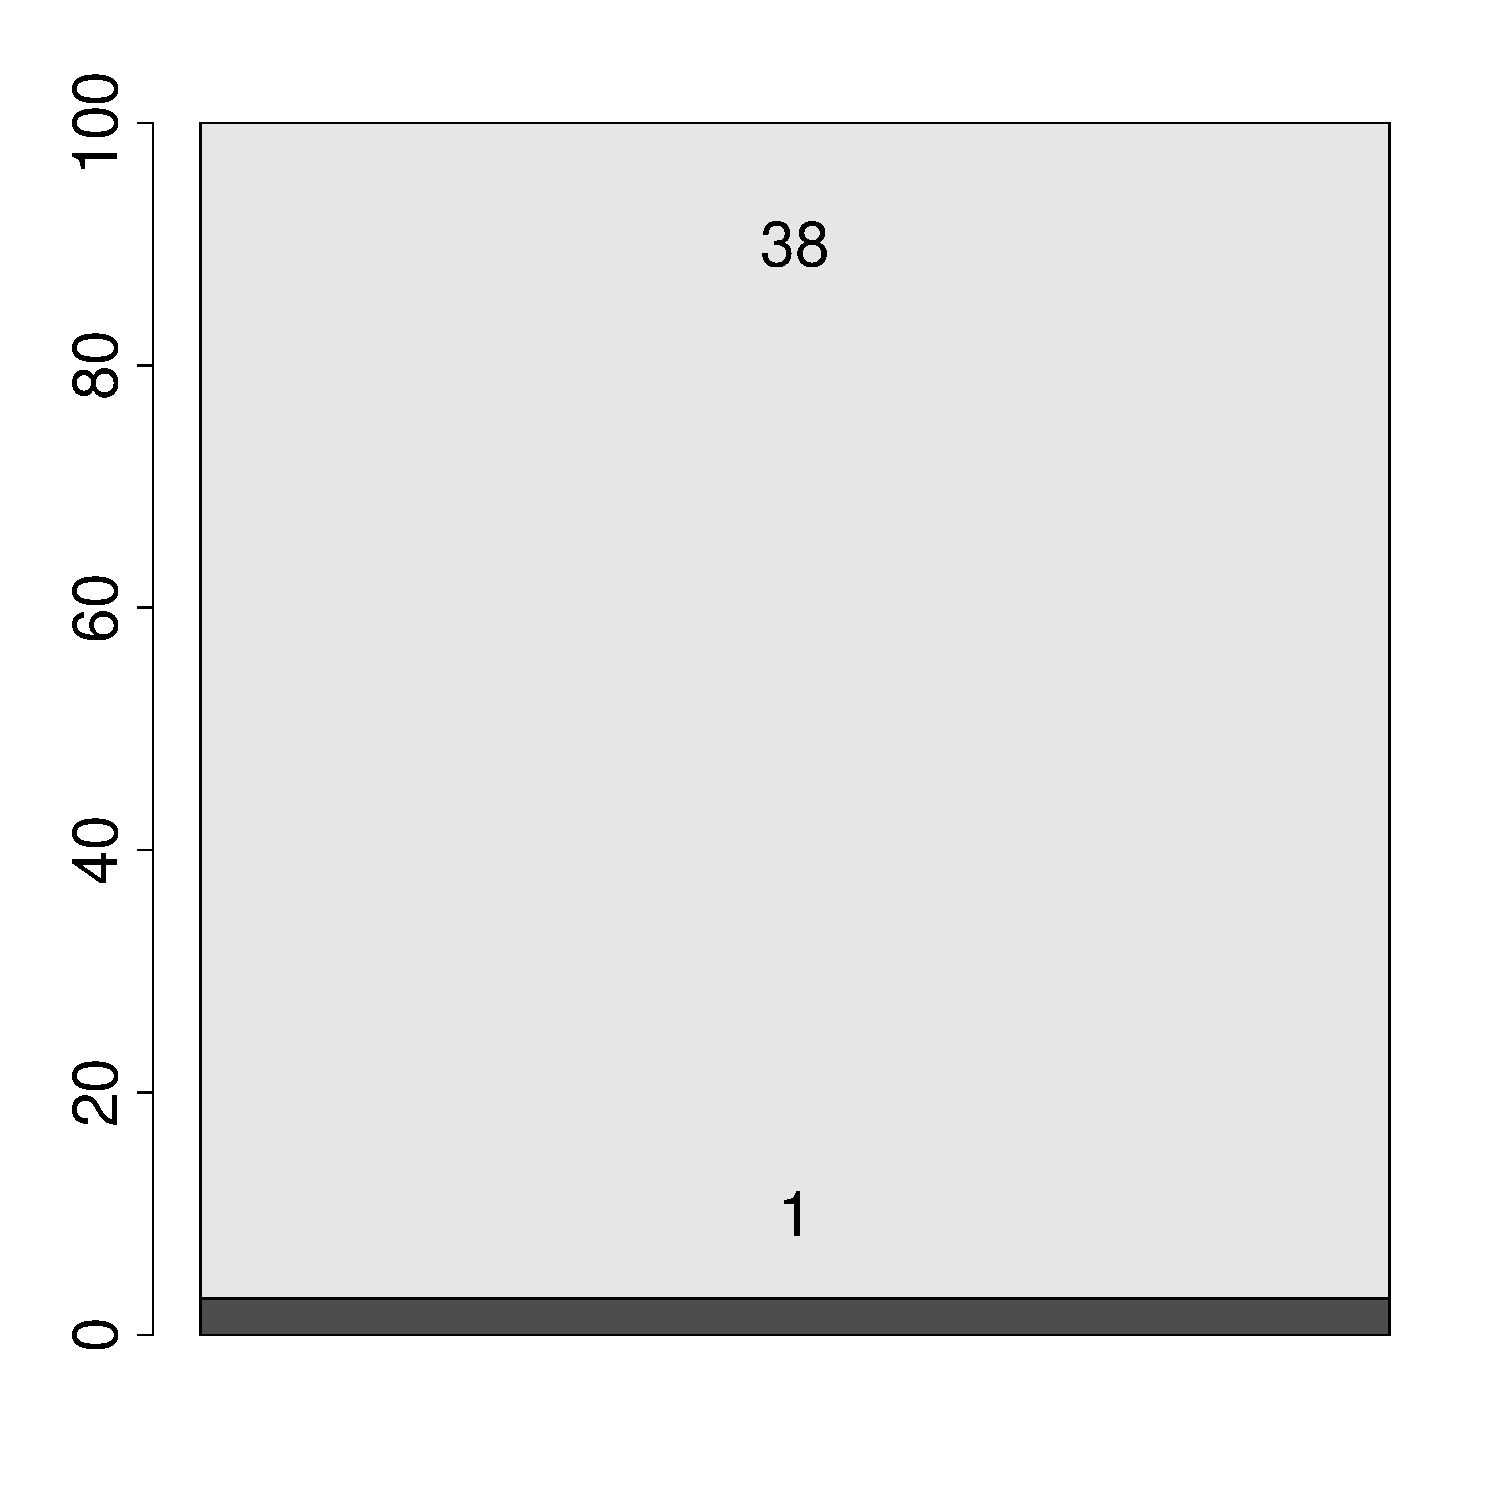
\includegraphics[height=.25\textheight]{generated/images/koerper-I}
% \caption {Isidor}
% \end{subfigure}%
% \begin{subfigure}[b]{.5\linewidth}
%   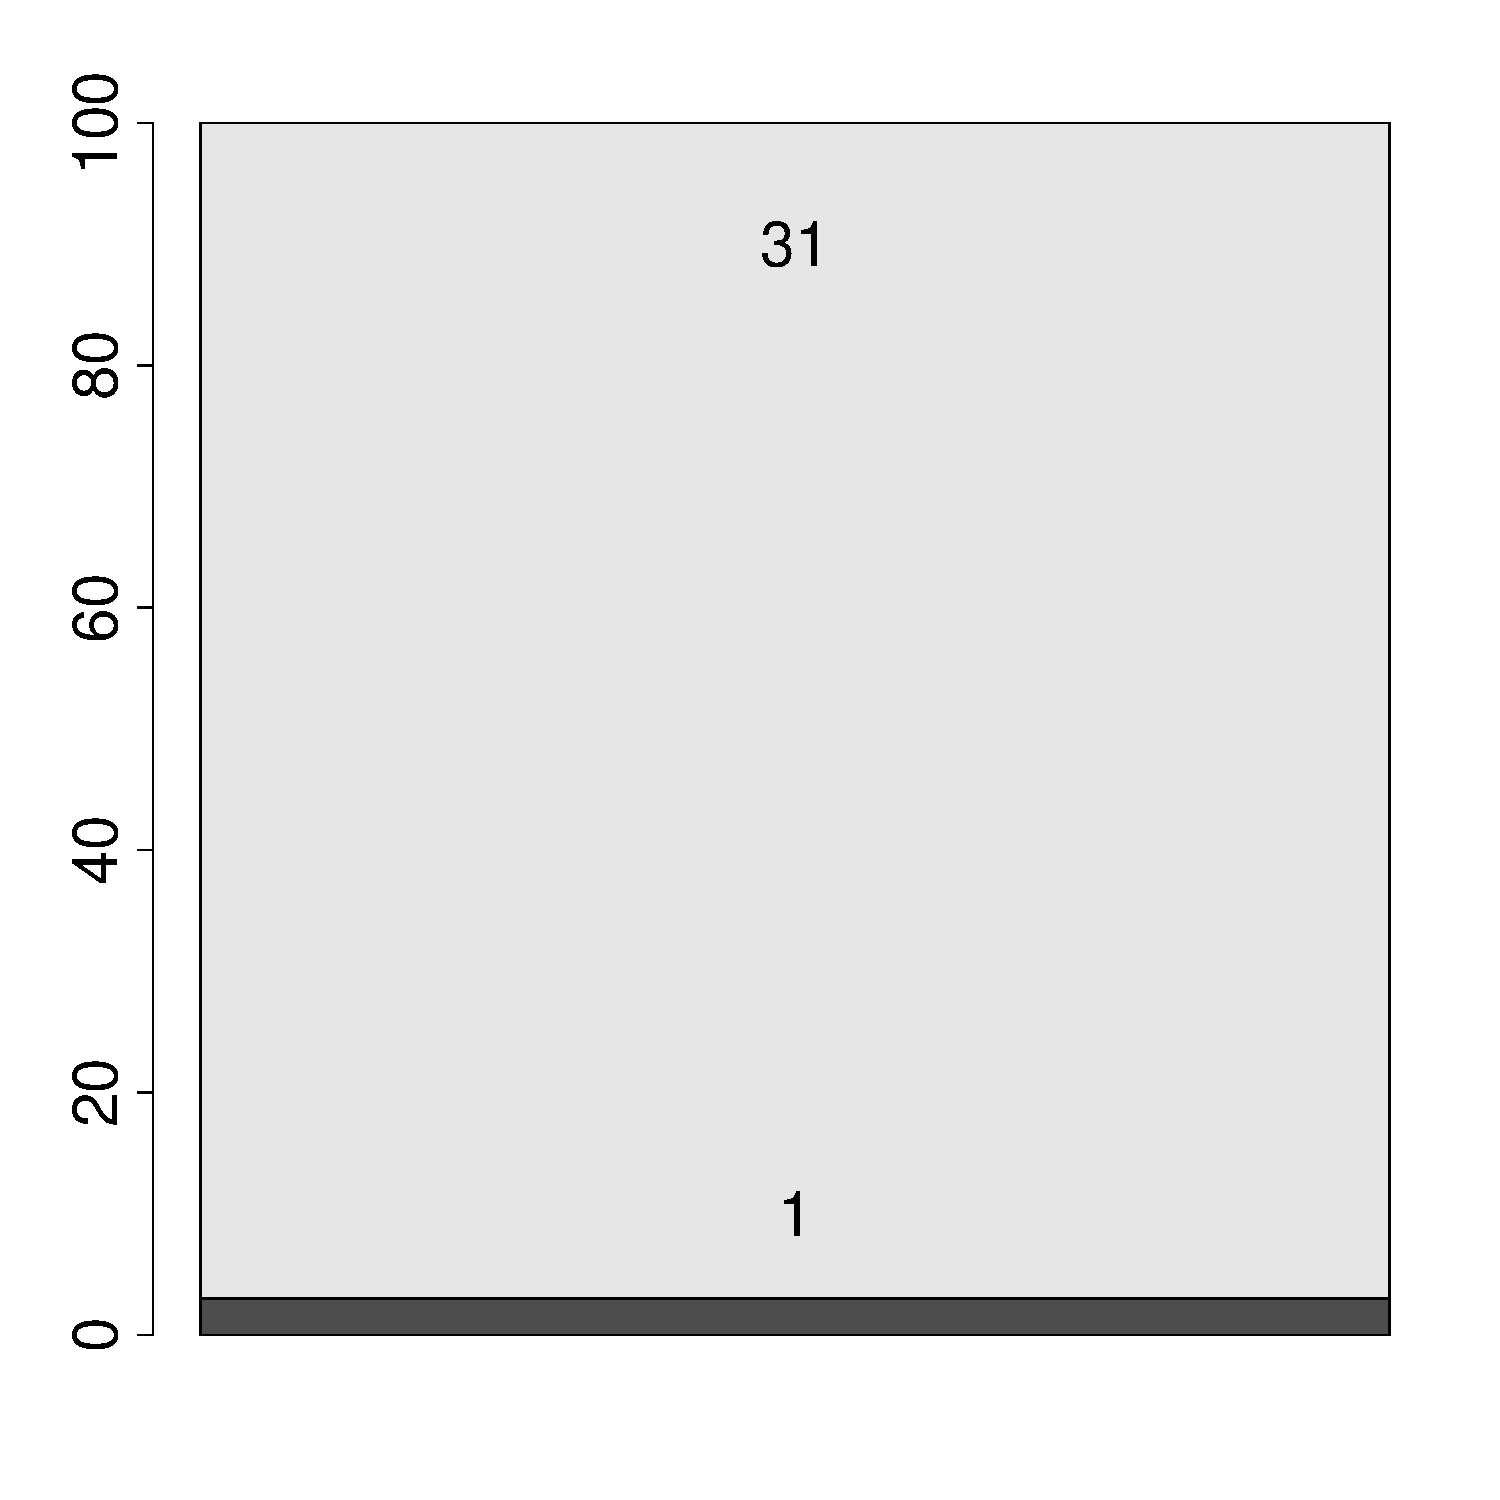
\includegraphics[height=.25\textheight]{generated/images/koerper-M}
% \caption {Monseer Matthäus}
% \end{subfigure}

% \begin{subfigure}[b]{.5\linewidth}
%   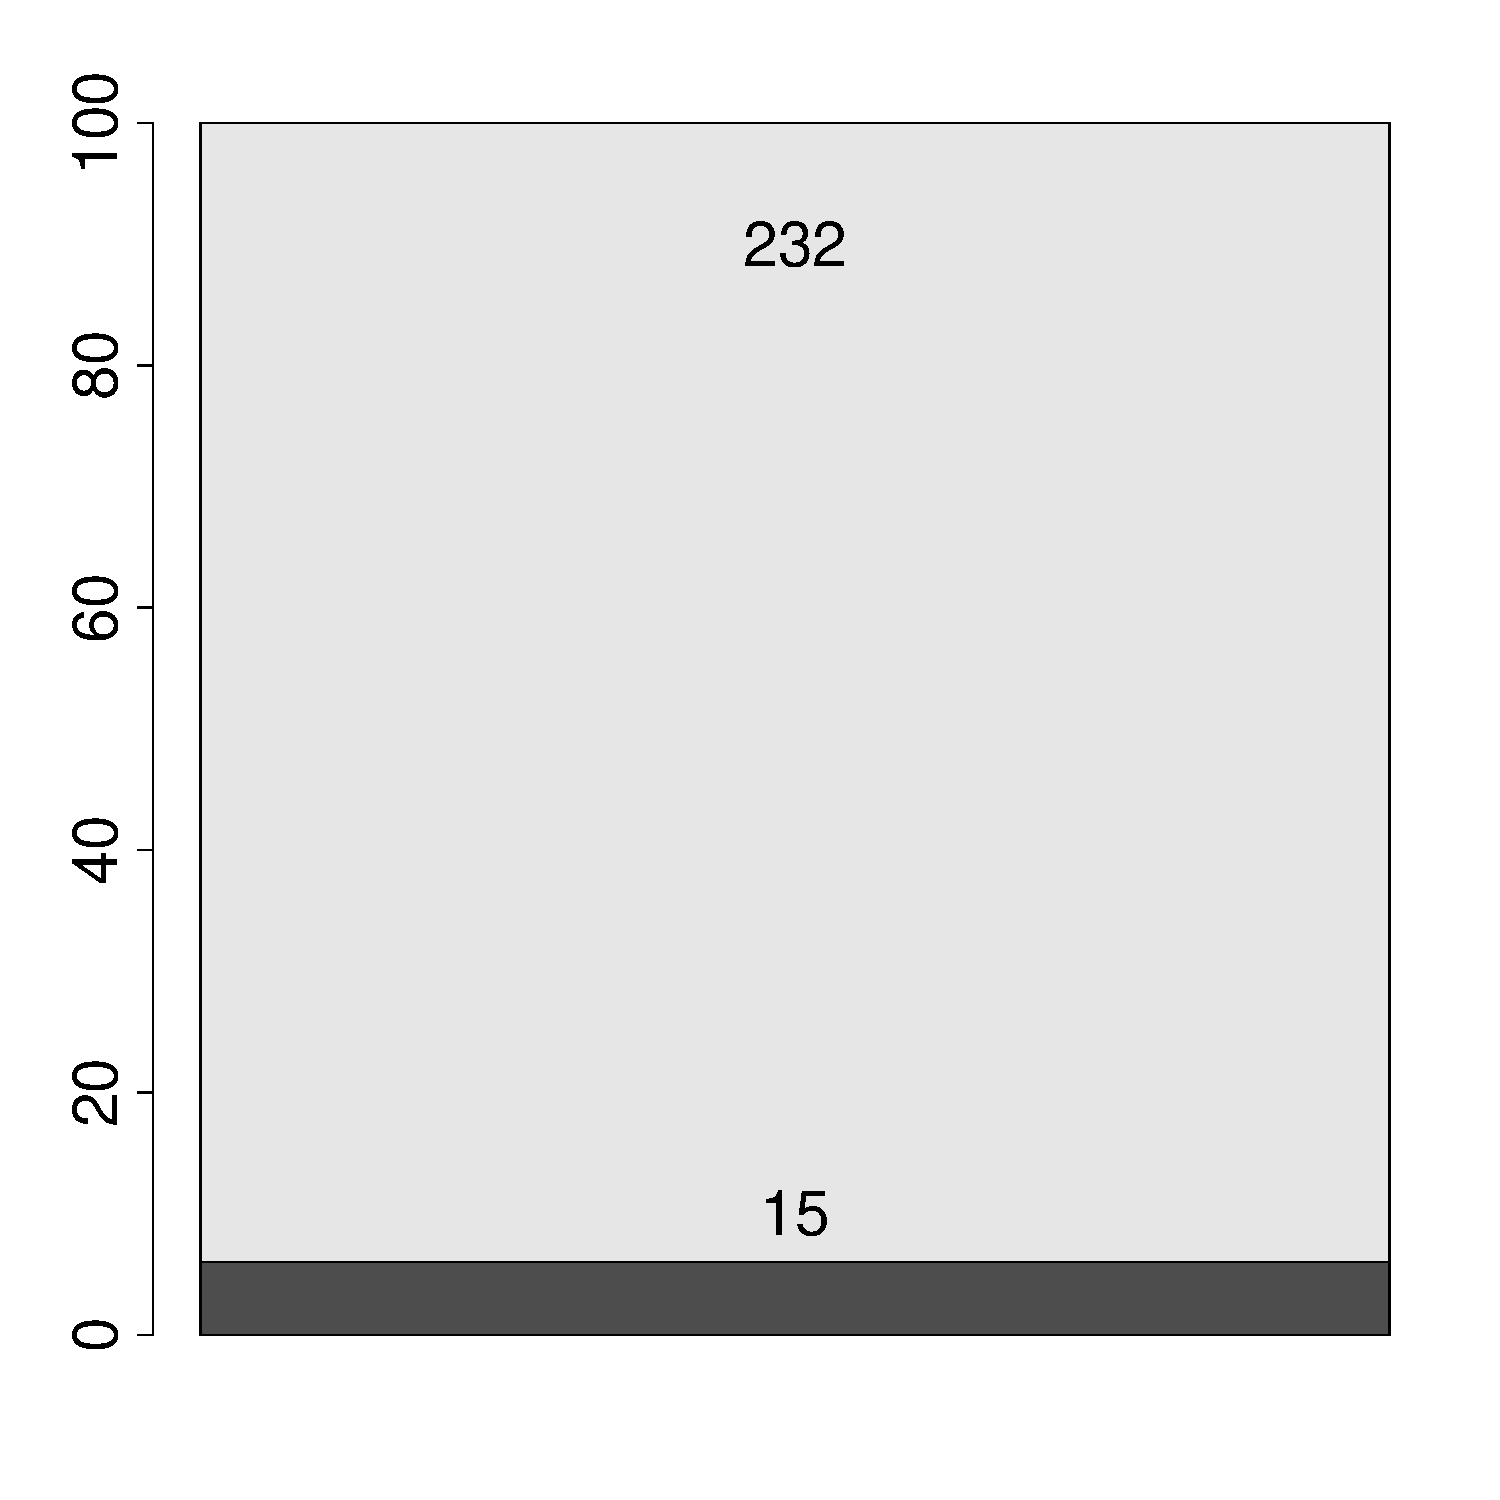
\includegraphics[height=.25\textheight]{generated/images/koerper-T}
% \caption {Tatian}
% \end{subfigure}%
% \begin{subfigure}[b]{.5\linewidth}
%   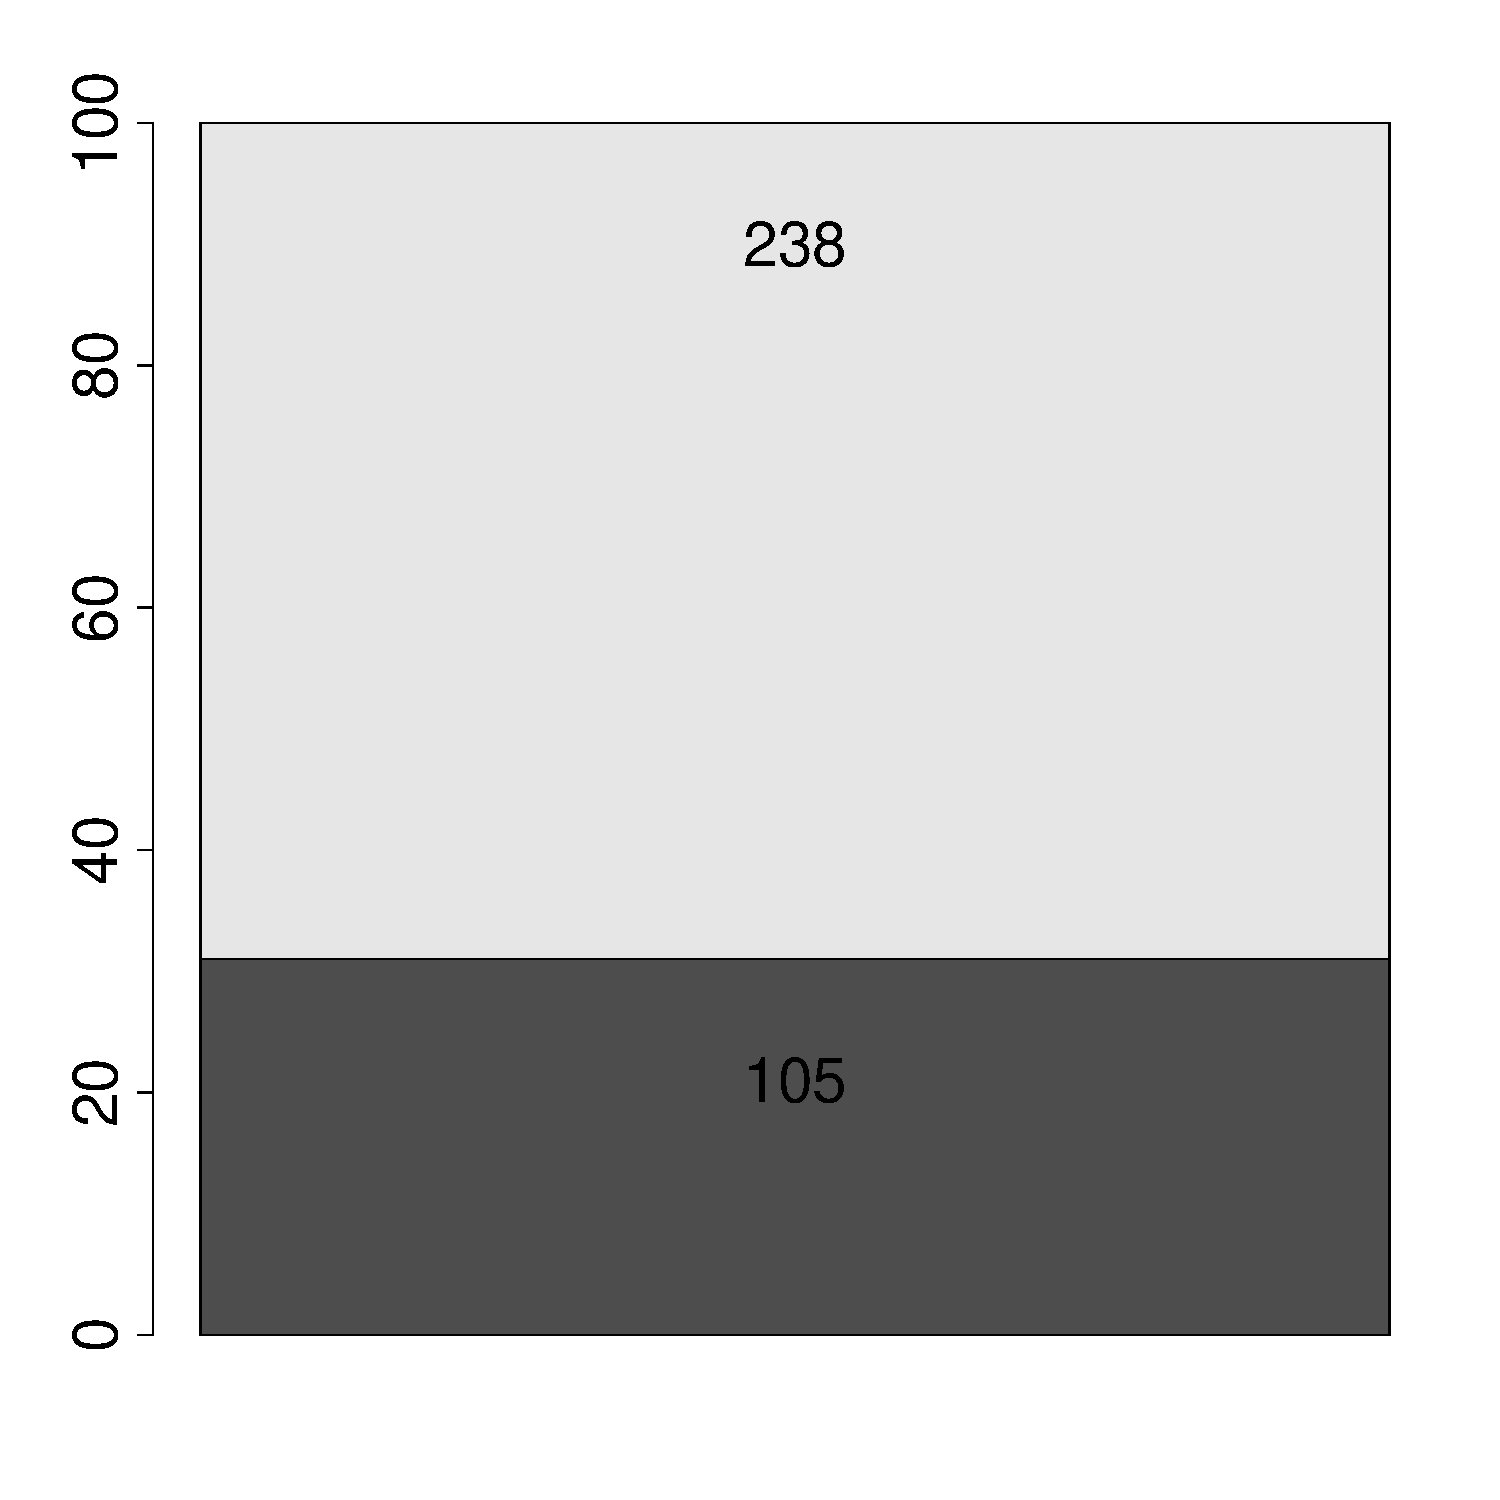
\includegraphics[height=.25\textheight]{generated/images/koerper-O}
% \caption {Otfrid}
% \end{subfigure}

% \begin{subfigure}[b]{.5\linewidth}
%   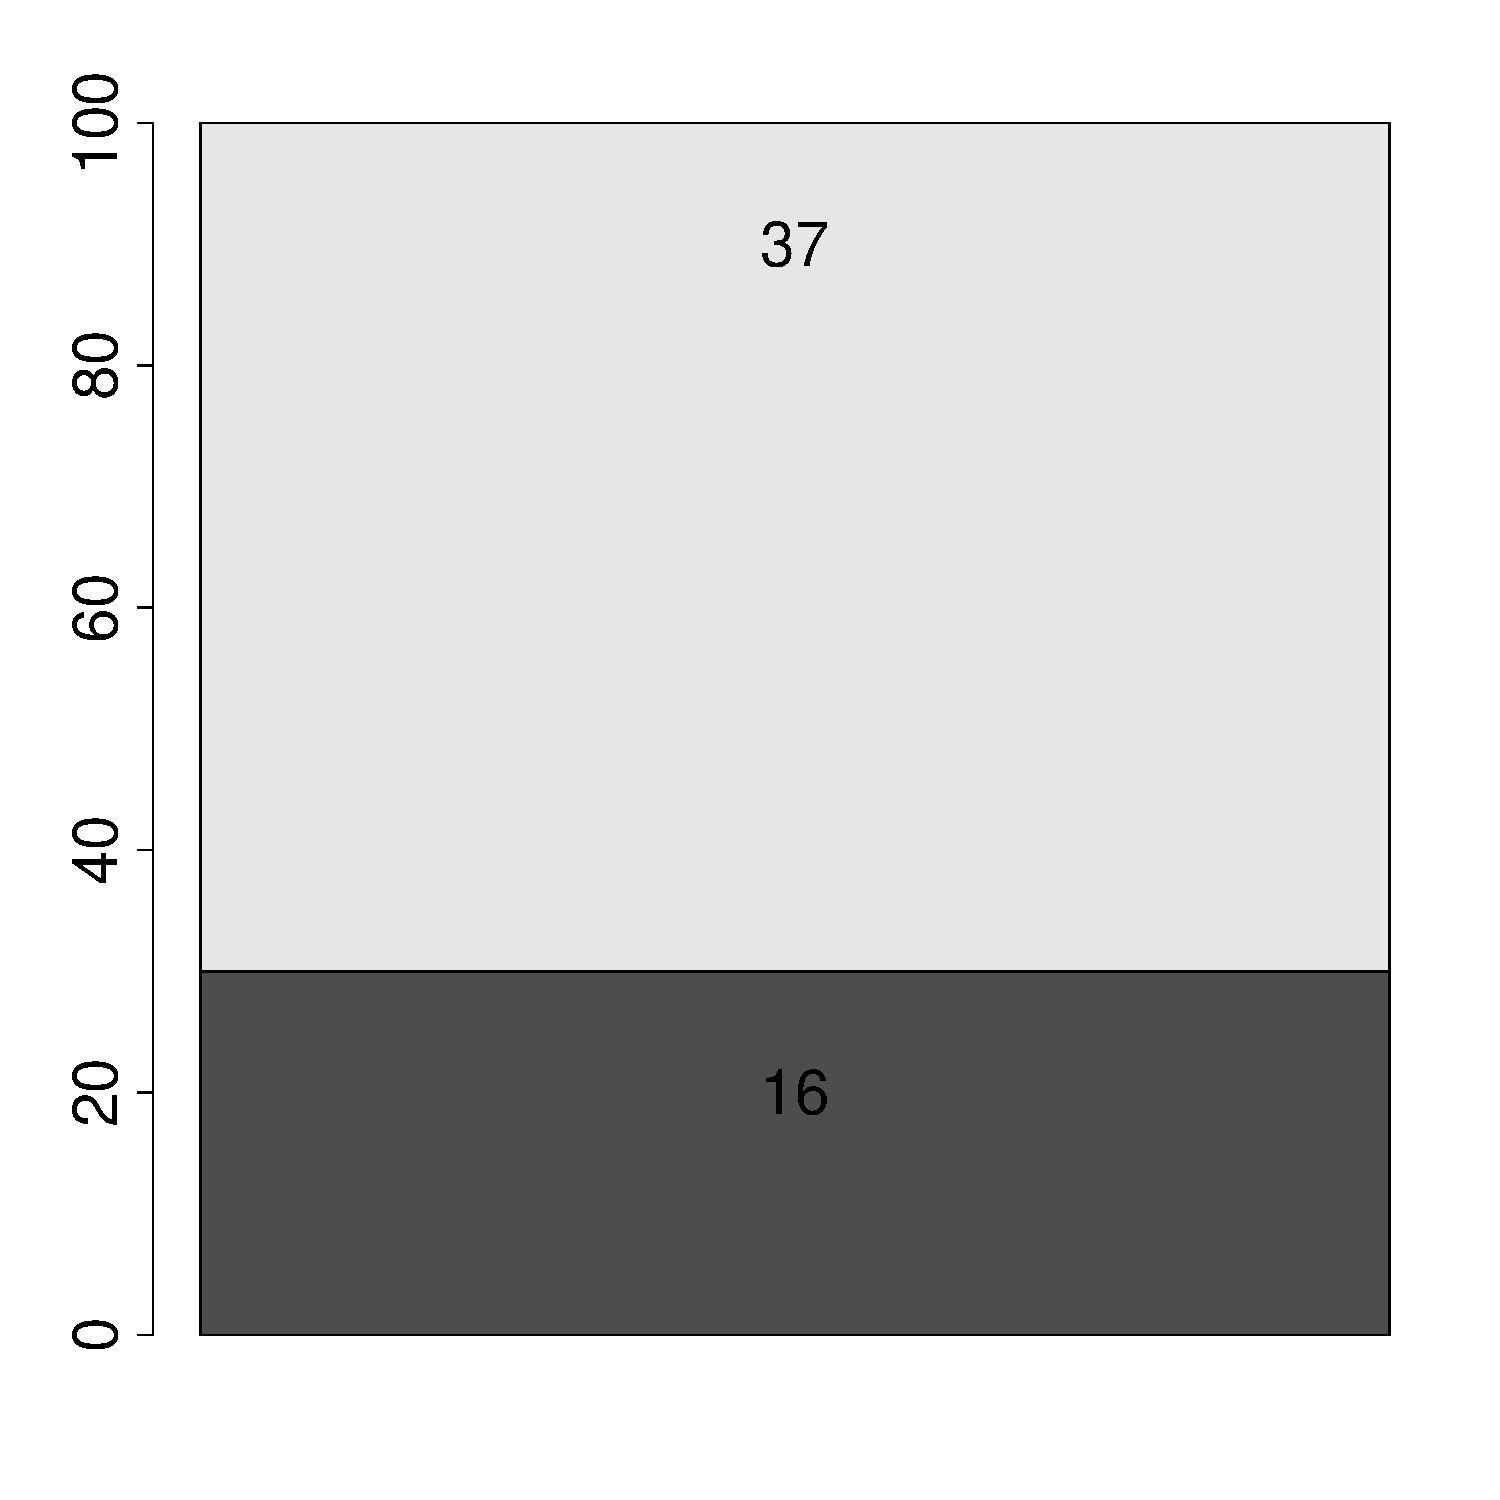
\includegraphics[height=.25\textheight]{generated/images/koerper-N}
% \caption {Notker}
% \end{subfigure}%
% \begin{subfigure}[b]{.5\linewidth}
%   
\includegraphics[height=.25\textheight]{generated/images/ort-legende}
% \end{subfigure}
% \caption{Gebrauch von \object{dër} bei Bezeichnungen für Körperteile}
% \label{fig:bel-koerper}
% \end{figure}

% %
%  \begin{figure}
% \begin{subfigure}[b]{.5\linewidth}
%   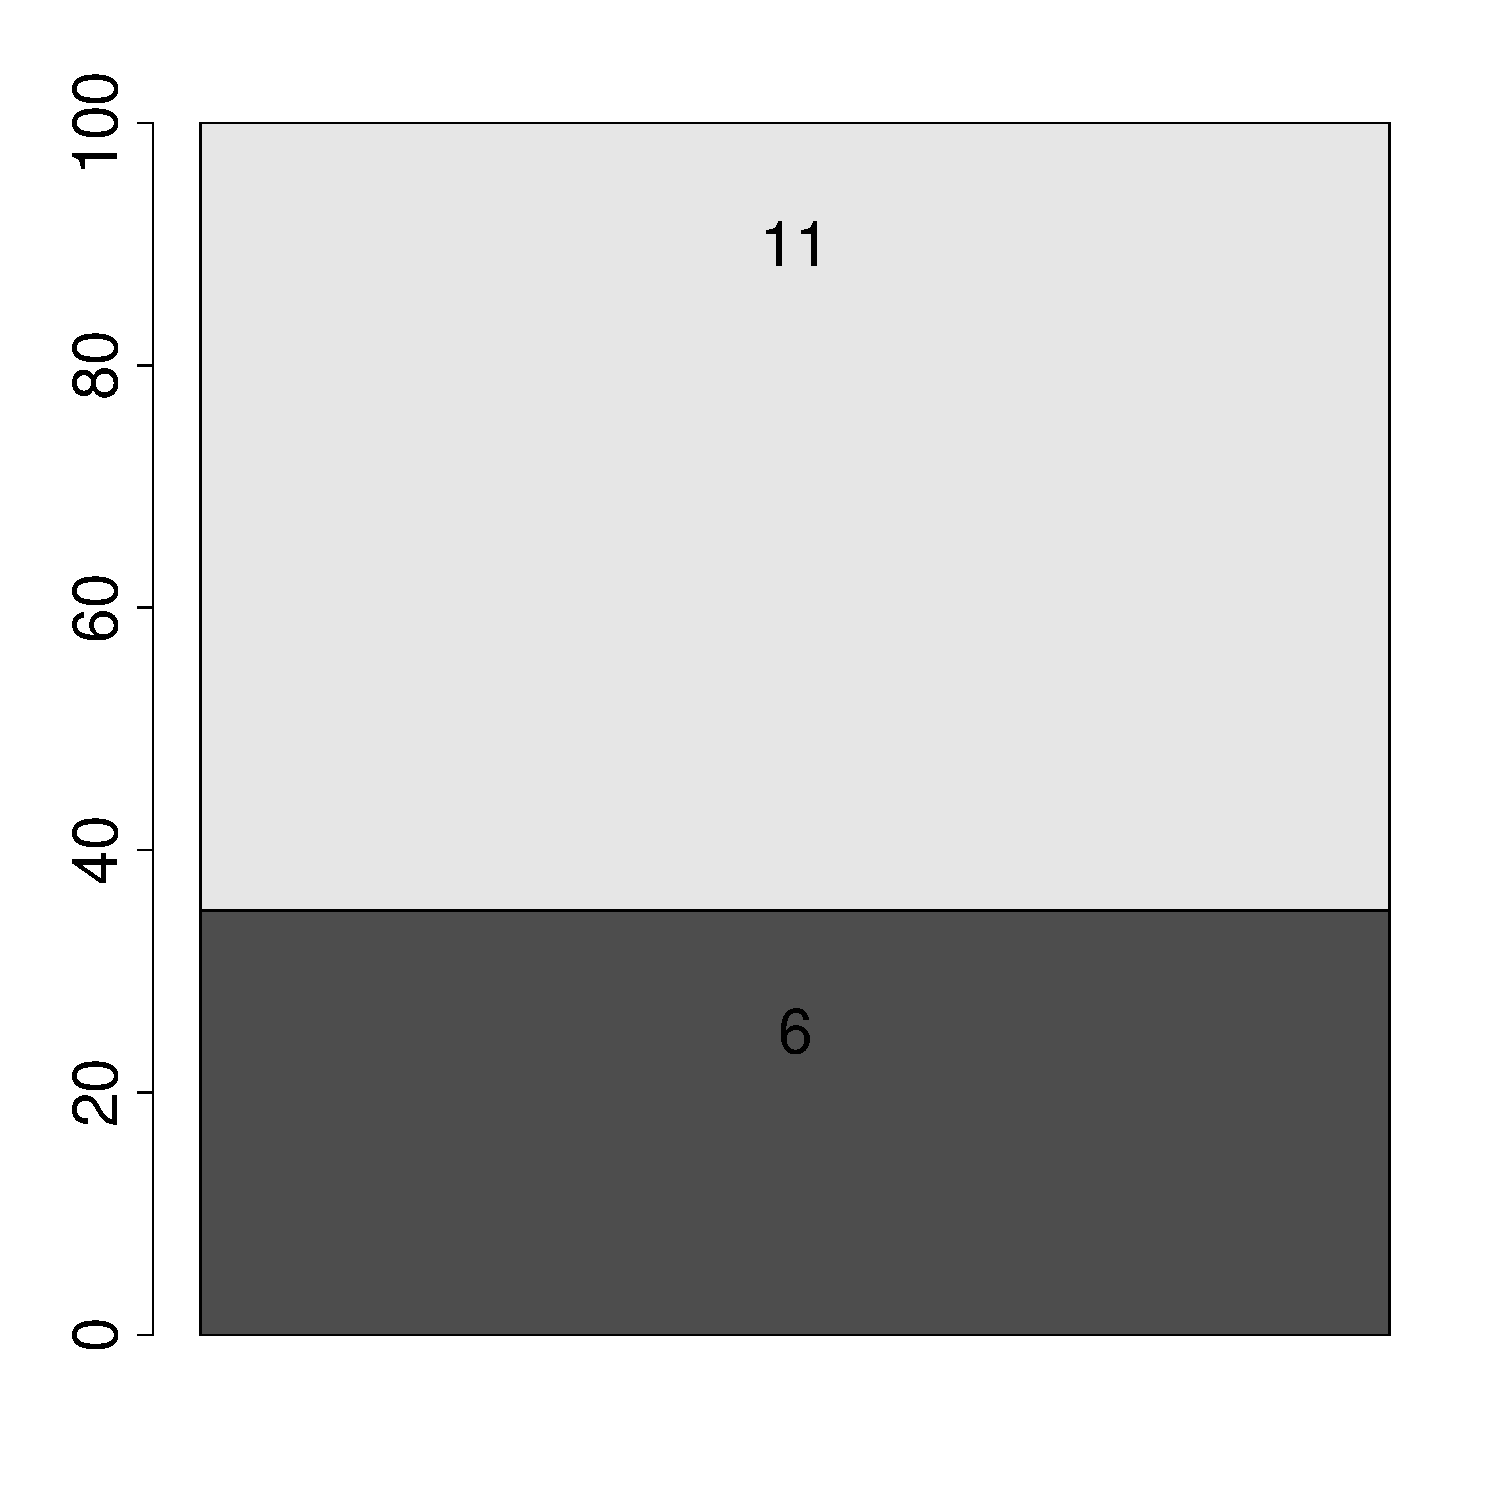
\includegraphics[height=.25\textheight]{generated/images/ort-I}
% \caption {Isidor}
% \end{subfigure}%
% \begin{subfigure}[b]{.5\linewidth}
%   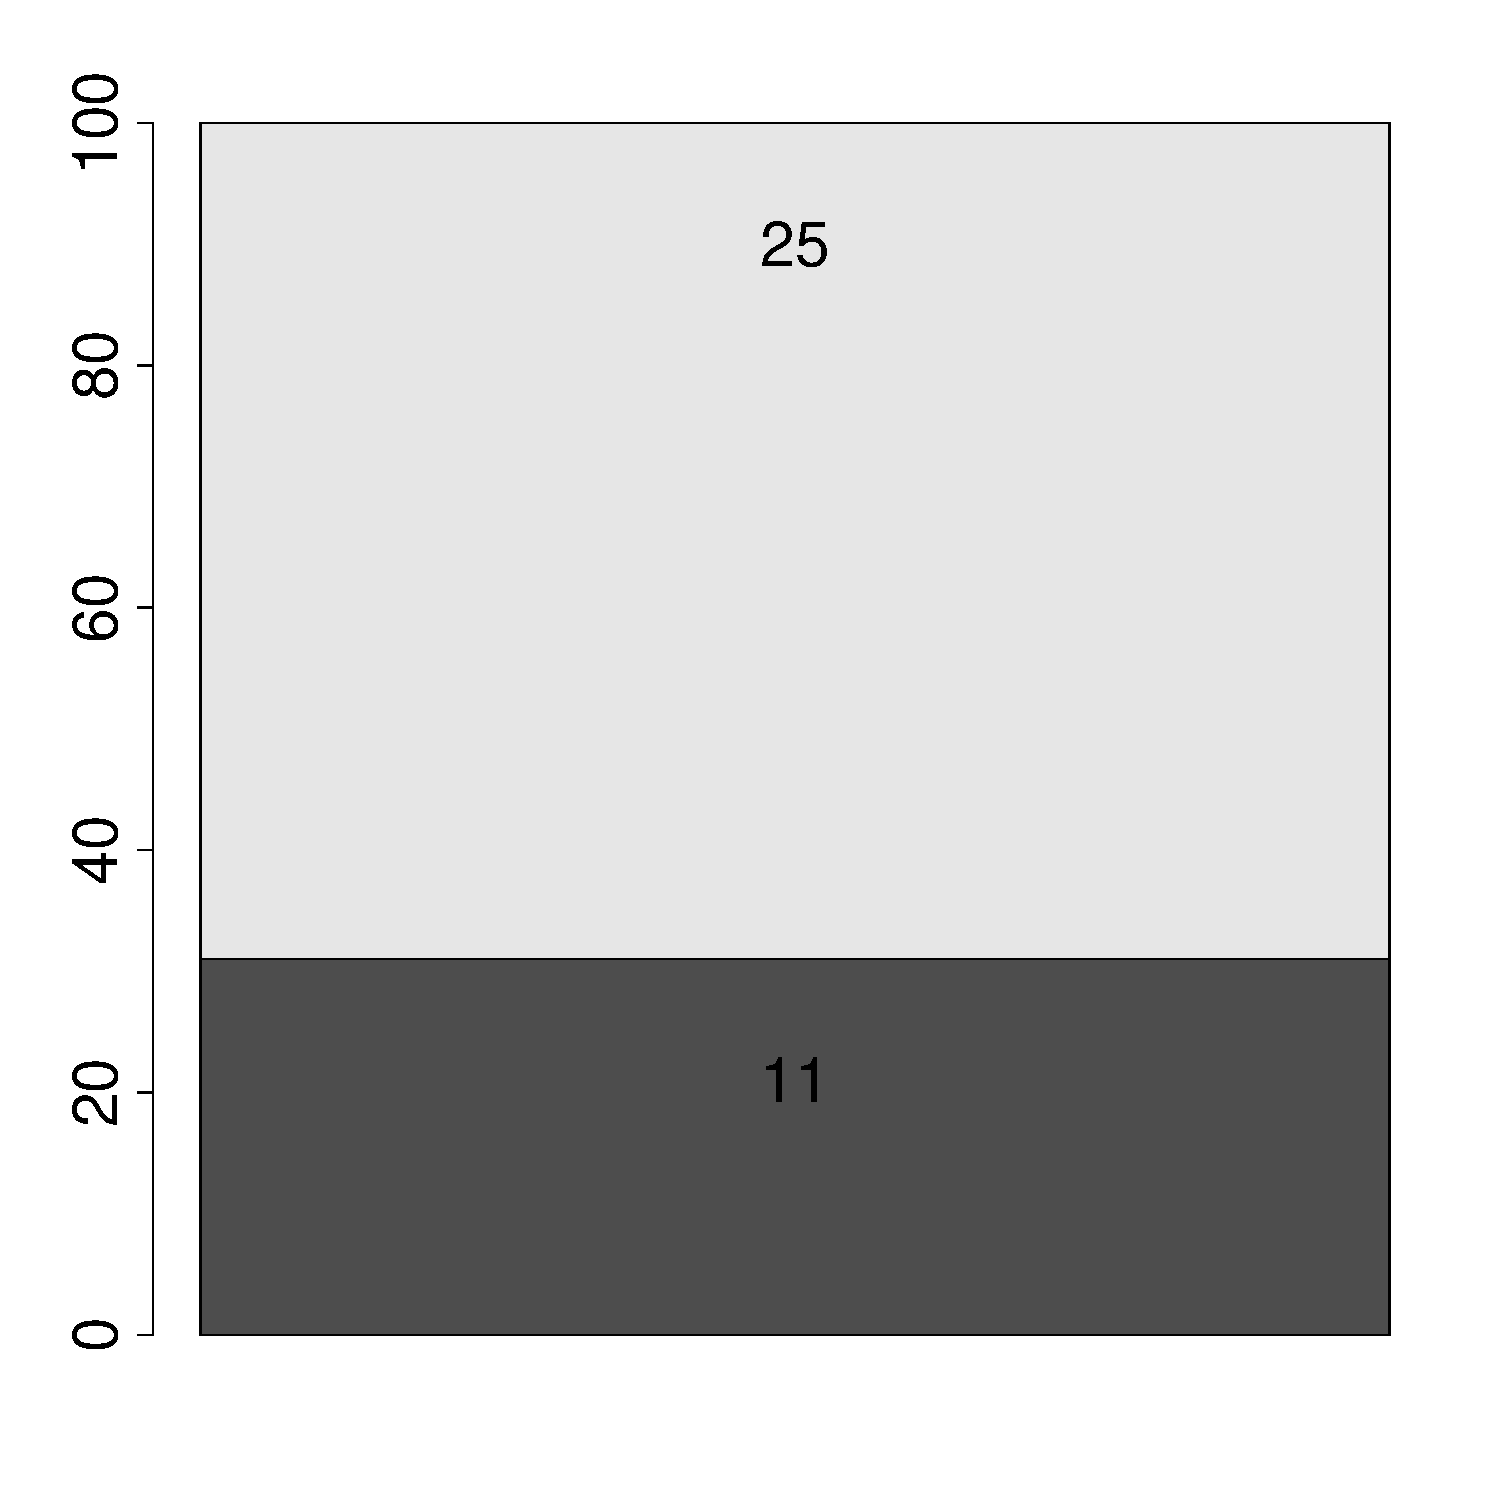
\includegraphics[height=.25\textheight]{generated/images/ort-M}
% \caption {Monseer Matthäus}
% \end{subfigure}

% \begin{subfigure}[b]{.5\linewidth}
%   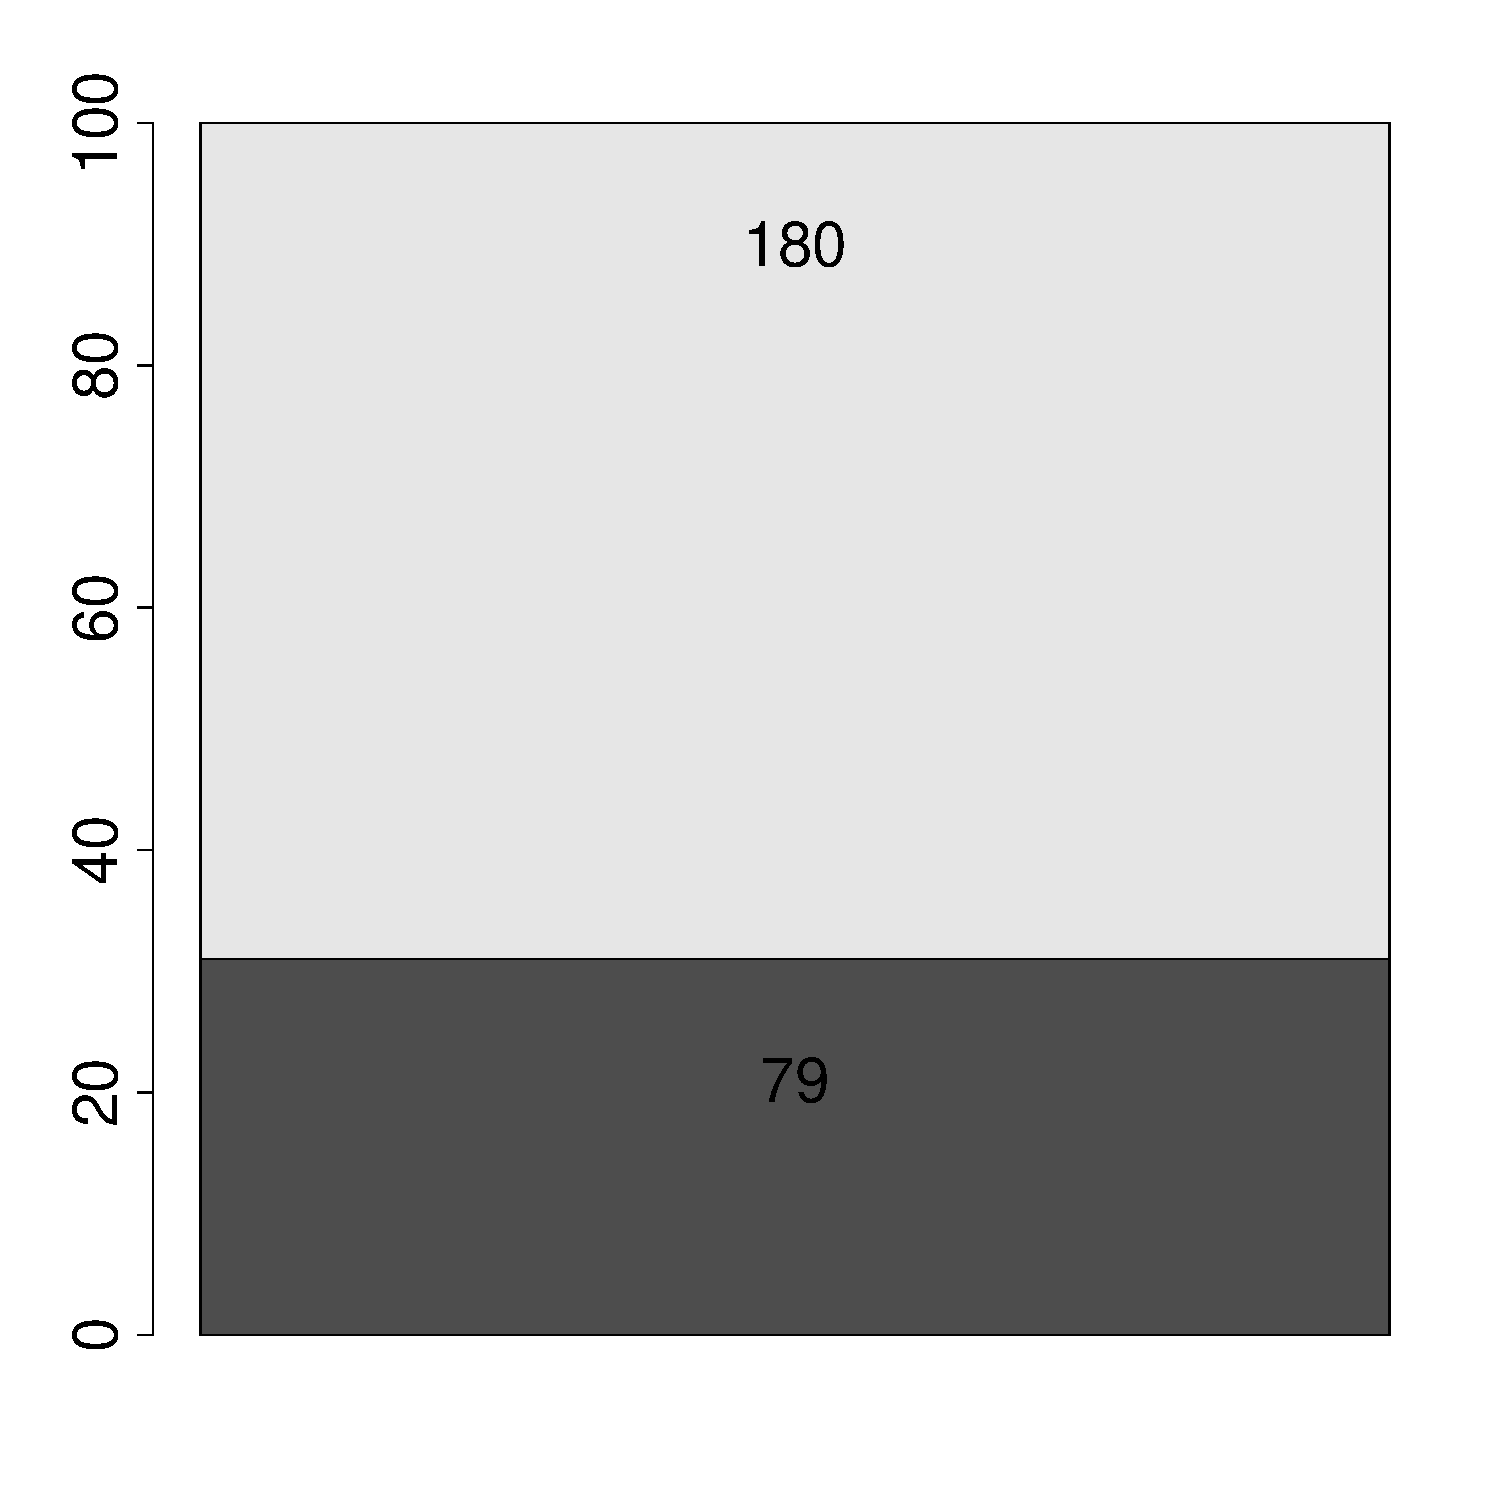
\includegraphics[width=6cm]{generated/images/ort-T}
% \caption {Tatian}
% \end{subfigure}%
% \begin{subfigure}[b]{.5\linewidth}
%   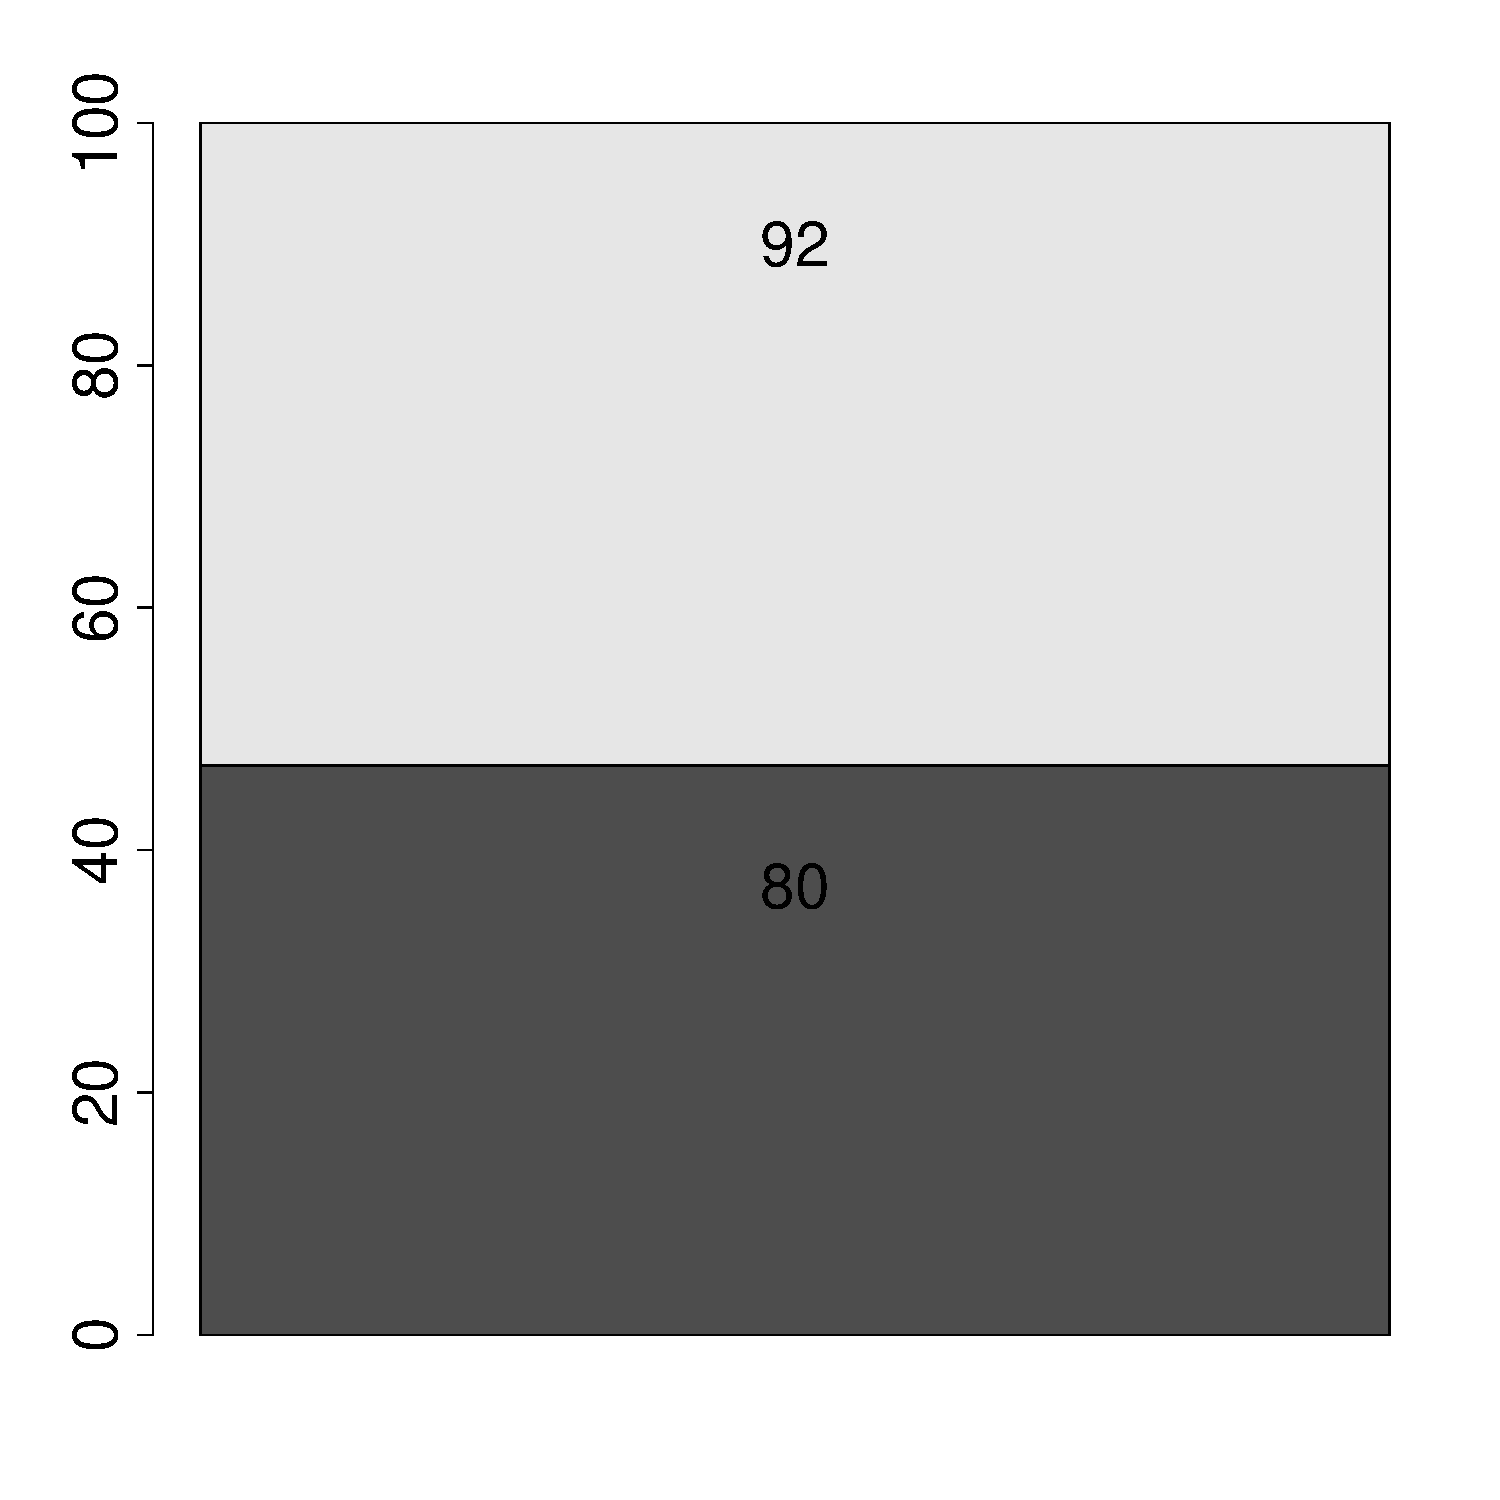
\includegraphics[height=.25\textheight]{generated/images/ort-O}
% \caption {Otfrid}
% \end{subfigure}

% \begin{subfigure}[b]{.5\linewidth}
%   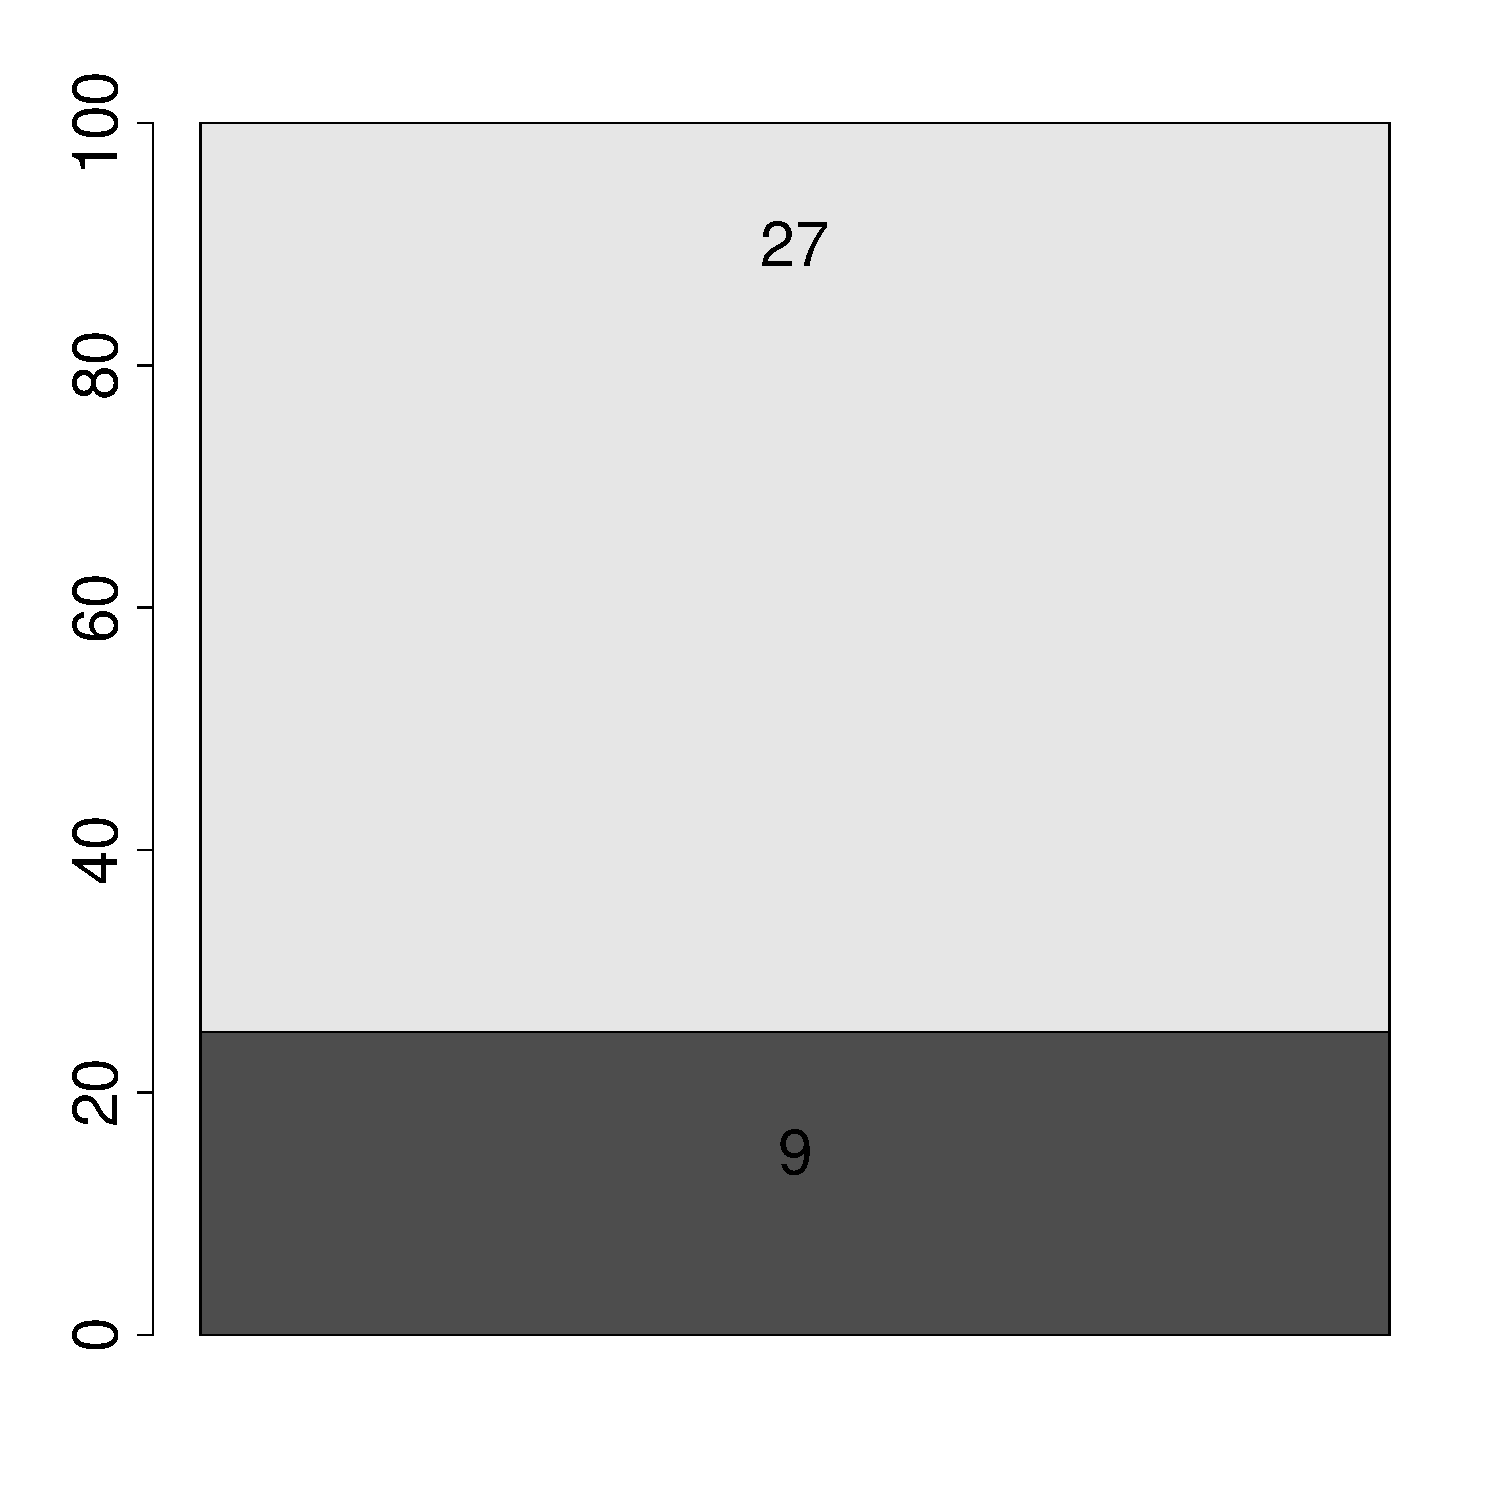
\includegraphics[height=.25\textheight]{generated/images/ort-N}
% \caption {Notker}
% \end{subfigure}%
% \begin{subfigure}[b]{.5\linewidth}
%   
\includegraphics[height=.25\textheight]{generated/images/ort-legende}
% \end{subfigure}
% \caption{Gebrauch von \object{dër} bei Ortsbezeichnungen}
% \label{fig:bel:orte}
% \end{figure}

\subsection{Individualität}\label{sec:ergeb-individualität}

Im Theorieteil der Arbeit (Abschnitt \ref{sec:indi}) wurden Parameter präsentiert, die die  \isi{Individualität} determinieren. Neben der Materialität (konkret vs. abstrakt), ist es die Zählbarkeit, welche dafür sorgt, dass ein Referent als distinktive Einheit wahrgenommen wird. Kontinuativa \is{Massennomen} (=\,Massennomen und Kollektiva) sind entsprechend weniger individualisiert als abgrenzbare pluralisierbare Einheiten.\linebreak Das Gleiche gilt für Referenten, die im Plural (also als Gruppe) erscheinen. Die nachfolgenden Ergebnisse zeigen erstens, inwiefern \object{dër} in den einzelnen Texten mit Kontinuativa kompatibel ist, und zweitens, ob sich signifikante Unterschiede zwischen Singular- und Pluralformen attestieren lassen.

%\subsubsection{Kontinuativa}

Analog zum Vorgehen bei den Unika \is{Unikum} (Abschnitt \ref{sec:ergeb-monosem}) wurde in allen Texten nach Lemmata \is{Lemma} gesucht, die typische Vertreter der zu untersuchenden Kategorie Kontinuativa repräsentieren. Um die Variable \isi{Belebtheit} auszublenden, wurden keine Kollektiva, sondern nur unbelebte Kontinuativa \is{Massennomen} ausgewählt. Die Auswahl ist dadurch begründet, dass die Nicht-Zählbarkeit von belebten Referenten offenbar nur wenig Einfluss auf die Determination hat. Dies verdeutlichen Kollektiva \is{Massennomen} wie \object{managi}, \object{folk} und  \object{liut}. Sie treten auch in den frühen Texten häufiger mit \object{dër} auf als ohne, vgl. die Lemmalisten \is{Lemma} in Abschnitt \ref{sec:ergeb-relevanz}. 

Um eine Vergleichbarkeit zwischen den Texten zu gewährleisten, wurde darauf geachtet, dass die Lemmata \is{Lemma} mit einer Tokenfrequenz \is{Token} von über 10 im Gesamtkorpus \is{Korpus} auftreten. Auf Basis der Untersuchungen von \textcite[28--29]{Graf1905}, \textcite[27--28]{Bell1907} und  \textcite[464]{Oubouzar1989} wurden die Lemmata \is{Lemma} \object{waʒʒar} \extrans{Wasser}, \object{gold} \extrans{Gold} und  \object{bluot} \extrans{Blut} ausgewählt; als Kontrolllemma \is{Lemma} dient das zählbare Nomen \object{stein} \extrans{Stein}. 

Tabelle~\ref{tab:wasser} zeigt die Häufigkeiten aller \object{waʒʒar}-Phrasen \is{Phrase} aufgeteilt nach Vorkommen mit und ohne \object{dër}. 

\begin{table}
\centering
\begin{tabular}{lrr}
\lsptoprule
{Text}  & {mit \object{dër}} & {ohne \object{dër}}  \\ \midrule
Isidor (790)           & 1  & 4     \\
Monseer Matthäus (810) & 0  & 0     \\
Tatian (840)           & 5  & 16    \\
Otfrid (870)           & 10 & 13    \\
Notker (1025)          & 2  & 4     \\ \lspbottomrule
\end{tabular}
\caption{\object{dër}-Setzung bei \object{waʒʒar} \extrans{Wassser}}
\label{tab:wasser}
\end{table}

Wie man sieht, dominieren in allen Texten die undeterminierten Belege. Die einzelne \object{dër}-Phrase \is{Phrase} im Isidor (\object{dhazs ir oba dhem uuazsserum suueiboda}, I 4,4) bezieht sich auf ein kurz zuvor genanntes Bibelzitat (\object{endi gotes gheist suueiboda oba uuazsserum}, I 4,4) und kann daher als eine pragmatisch motivierte Anapher \is{anaphorisch}\is{Pragmatische Definita}betrachtet werden \parencite[vgl. auch][110]{Oubouzar1989}. Aber auch eine abstrakt-situative \is{abstrakt-situativ} Lesart (\extrans{über das Wasser/Meer}) ist hier nicht auszuschließen.\largerpage[-1]

%, vgl. \REF{ex:I2244}.  
%\begin{exe}
\ex \label{ex:I2244} \gll \object{In dhiu} \object{auh} \object{dhanne} \object{0} \object{dhazs} \object{ir} \object{oba} \object{\underline{dhem}} \object{uuazsserum} \object{suueiboda} \object{0} \object{dhen} \object{heilegun} \object{gheist} \object{dhar} \object{bauhnida} \object{. } \\
{dabei} {auch} {damals} {} {dass} {er} {auf} {der} {Wasser} {sich bewegen} {} {der} {heilig} {Geist} {da} {zeigen} {}\\
\glt TODO: nhd. Übersetzung (I.4,4)
\end{exe}


Die Durchsicht der einzelnen Belege lässt vermuten,  dass  \object{dër}  eher gebraucht wird, wenn \object{waʒʒar} ein konkretes Gewässer, etwa das Meer oder einen Fluss denotiert. Ausgehend von den kontextsensitiven Übersetzungen im \isi{Korpus} steht \extrans{Wasser} für 9 determinierte und 23 undeterminierte Token. Wird \object{waʒʒar} zusätzlich mit \extrans{Meer}, \extrans{Fluss} oder \extrans{Bach} übersetzt, so verschiebt sich das Verhältnis leicht: 9 zu 14. Allerdings ist dieser Unterschied nicht signifikant (Exakter Test nach Fisher: $p=0{,}56$). Den Analysen von \textcite[464]{Oubouzar1989} zufolge steht \object{dër} bei individualisierten Einheiten und fehlt, wenn eine generische Lesart vorliegt. 


Das \isi{Lemma} \object{gold} kommt überwiegend ohne definites Artikelwort vor, s. Tabelle~\ref{tab:gold}; zukünftige qualitative Analysen müssten zeigen, inwiefern auch hier generischer \is{generisch} Gebrauch vorliegt. 
   
\begin{table}
\centering
\begin{tabular}{lrr}
\lsptoprule
{Text}  & {mit \object{dër}} & {ohne \object{dër}}  \\ \midrule
Isidor (790)           & 0  & 0     \\
Monseer Matthäus (810) & 2  & 1     \\
Tatian (840)           & 1  & 3     \\
Otfrid (870)           & 0  & 5     \\
Notker (1025)          & 0  & 4     \\ \lspbottomrule
\end{tabular}
\caption{\object{dër}-Setzung bei \object{gold} \extrans{Gold}}
\label{tab:gold}
\end{table}

%Zur Illustration ist in \REF{ex:N31557} ein Beispiel aus dem jüngsten Text (Notker) aufgeführt. 
%\begin{exe}
\ex \label{ex:N31557} \gll \object{dô} \object{sie} \object{íro} \object{\underline{gólt}} \object{púten} \object{. } \\
{da} {er} {er} {Gold} {anbieten} {}\\
\glt TODO: nhd. Übersetzung (N.2,102)
\end{exe}
 

Nur im Monseer Matthäus sowie im Tatian finden sich \object{gold}-Belege mit \object{dër}. Die nachfolgenden Übersetzungsstellen zeigen besonders gut, dass die Determinierung pragmatisch \is{Pragmatische Definita} genutzt wird. Während im Monseer Matthäus ein \object{dër} gesetzt wird, um lat. \object{in aurum templi} zu übersetzen, nutzt der Tatianübersetzer eine \is{Phrase} \object{dër}-Phrase, um \object{per templum} wiederzugeben. Mit \object{dër} wird also jeweils die andere Seite des Kontrastes ausgezeichnet -- im Monseer Matthäus ist es das Gold des Tempels, das im Vordergrund steht, im Tatian der Tempel selbst. 

\begin{exe}
\ex
lat. quicumque iuraverit per templum nihil est, qui autem iuraverit in aurum templi debet 
\sn \extrans{Wer da schwört bei dem Tempel, der ist nichts, wer aber bei dem Gold des Tempels schwört, der ist schuldig.}
\begin{xlist}
\ex \label{ex:gold-M} \gll  {so huuer so} {bi} {tem ple} {suerit} {neo uuiht} {sii}, {Der} {auuar} {\textit{in}} {\textit{demo}} {\textit{tem ples}} {\textit{golde}} {suerit}  {scul dic}  {eidh}  {sii}  \\
{jeder der} {bei} {Tempel} {schwört} {nichts} {sei}, 
{der} {aber} {in} {dem} {Tempels} {Gold} {schwört} {schuldig} {Eid} {sei} (M 17,1)\\

\ex \label{ex:gold-T} \gll 
{so uuer so} {suerit} {\textit{bi}} {\textit{themo}} {\textit{temple}} {ther} {n nist} {niouuiht}, {ther} {de} {suerit} {in}  {gold} {temples} {scal} \\
{Wer} {schwört} {bei} {dem} {Tempel} {der} {nicht ist} {nichts},
{der} {da} {schwört} {in} {Gold} {Tempels} {(ist) schuldig} (T 141,14)\\
\end{xlist}
\end{exe}

Im weiteren Text wird in beiden Übersetzungen das Gold des Tempels zweimal anaphorisch \is{anaphorisch} aufgenommen und auch hier sieht man unterschiedliche Übersetzungsverfahren: Im Tatian wird die erste Anapher \is{anaphorisch} mit \object{dër} wiedergegeben (\object{uuedar ist mera, thaz gold oda templum thaz dar heilagot gold?}, T 141,14),
im Monseer Matthäus ist es die zweite (\object{huuedar ist za uuare mera  gold odo kirihha diu daz golth uuihit?}, M 17,6), sinngemäß: \extrans{Was ist mehr wert, das Gold oder die Kirche, die das Gold heiligt?}. 
%\begin{exe}
\ex \label{ex:T28605} \gll \object{ther} \object{de} \object{suerit} \object{in} \object{gold} \object{\underline{temples}}  \\
{der} {da} {schwören} {in} {Gold} {Tempel}  {}\\
\glt TODO: nhd. Übersetzung (T.141,14)
\end{exe}

%\begin{exe}
\ex \label{ex:T28617} \gll \object{Dumbe} \object{inti} \object{blinte} \object{0} \object{uuedar} \object{ist} \object{mera} \object{0} \object{thaz} \object{\underline{gold}} \object{oda} \object{templum} \object{thaz} \object{dar} \object{heilagot} \object{gold} \object{?} \\
{dumm} {und} {blind} {} {wer} {sein} {mehr} {} {der} {Gold} {oder} {Tempel} {der} {da} {heiligen} {Gold} {}\\
\glt TODO: nhd. Übersetzung (T.141,14)
\end{exe}


Interessant ist der Vergleich von \object{gold} mit einem zählbaren Referenten wie  \object{stein}, s. Tabelle~\ref{tab:stein}. Die Wahrscheinlichkeit einer \object{dër}-Setzung ist hier höher: Bei \object{gold} liegt das Verhältnis von determinierten zu undeterminierten \isi{Token} bei 3 zu 13, d.h. jedes fünfte \isi{Token} trägt ein \object{dër}; bei \object{stein} ist es mit 19 zu 34 jedes dritte. 

\begin{table}
\centering
\begin{tabular}{lrr}
\lsptoprule
{Text}  & {mit \object{dër}} & {ohne \object{dër}} \\ \midrule
Isidor (790)           & 0  & 0     \\
Monseer Matthäus (810) & 0  & 0     \\
Tatian (840)           & 7  & 21    \\
Otfrid (870)           & 10 & 12    \\
Notker (1025)          & 2  & 1     \\ \lspbottomrule
\end{tabular}
\caption{\object{dër}-Setzung bei \object{stein} \extrans{Stein}}
\label{tab:stein}
\end{table}

Die nachfolgenden Tabellen zeigen die Verteilung von \object{dër} bei \object{bluot}. Auch bei diesem \isi{Massennomen} dominiert die undeterminierte Variante. Nur bei eindeutiger Referenz \is{Referentialität} steht ein \object{dër}, so etwa im Tatian, wenn von Pilatus' Blut die Rede ist \object{thero bluot Pilatus} (T, 102,1) oder im Monseer Matthäus, wo \extrans{das gerechte Blut} mit einem \isi{Adjektiv} und einem restrinktiven Relativsatz näher spezifiziert wird: \object{al daz reht ·  uuisiga bluoth · daz ubar ærda ist ka gozan} (M, 18,20--21).

%\begin{exe}
\ex \label{ex:M3723} \gll \object{*** } \object{chauf tun} \object{mit} \object{dem} \object{***} \object{z enes} \object{*** } \object{za} \object{grabum} \object{; } \object{Bidiu} \object{ist} \object{kanemnit} \object{*** } \object{daz} \object{ist} \object{\underline{bluotes}} \object{acchar} \object{untaz} \object{hiu tu} \object{Duo} \object{uuard} \object{arfullit} \object{daz} \object{kaquetan} \object{ist} \object{durah} \object{hieremiam} \object{den} \object{fora sagun} \object{Enti} \object{ant ·\fengun} \object{drizuc} \object{pendingo} \object{*** } \object{uuerdh} \object{daz} \object{sie} \object{ghachurun} \object{fona} \object{*** } \object{gabun} \object{dea} \object{uuidar} \object{demo} \object{hauuanares} \object{*** } \object{so} \object{mir} \object{kabot} \\
{} {kaufen} {mit} {der} {} {} {} {zu} {Grab} {} {deshalb} {sein} {benennen} {} {der} {sein} {Blut} {Acker} {bis} {heute} {da} {werden} {erfüllen} {der} {sprechen} {sein} {durch} {Jeremias} {der} {Prophet} {und} {empfangen} {dreißig} {Pfenning} {} {Wert} {der} {er} {auswählen} {von} {} {geben} {der} {wider} {der} {Töpfer} {} {so} {ich} {gebieten}\\
\glt TODO: nhd. Übersetzung (M.18,NA)
\end{exe}
 

\begin{table}
\centering
\begin{tabular}{lrr}
\lsptoprule
{Text}  & {mit \object{dër}} & {ohne \object{dër}} \\ \midrule
Isidor (790)           & 0  & 0     \\
Monseer Matthäus (810) & 2  & 6     \\
Tatian (840)           & 1  & 16    \\
Otfrid (870)           & 0  & 10    \\
Notker (1025)          & 2  & 0     \\ \lspbottomrule
\end{tabular}
\caption{\object{dër}-Setzung bei \object{bluot} \extrans{Blut}}
\label{tab:blut}
\end{table}


%\subsubsection{Numerus}

Da Referenten im Singular individuierter sind als Referenten, die im Plural auftreten (vgl. Abschnitt \ref{section:mass}), wurde auch der \isi{Numerus} als Variable für \isi{Individualität}  betrachtet. In Abbildung~\ref{fig:numerus} sind alle Appellativa \is{Gattungsname} aufgeteilt nach \isi{Numerus} und \object{dër}-Gebrauch abgebildet.

\begin{figure}[p]
\begin{subfigure}[b]{.5\linewidth}
  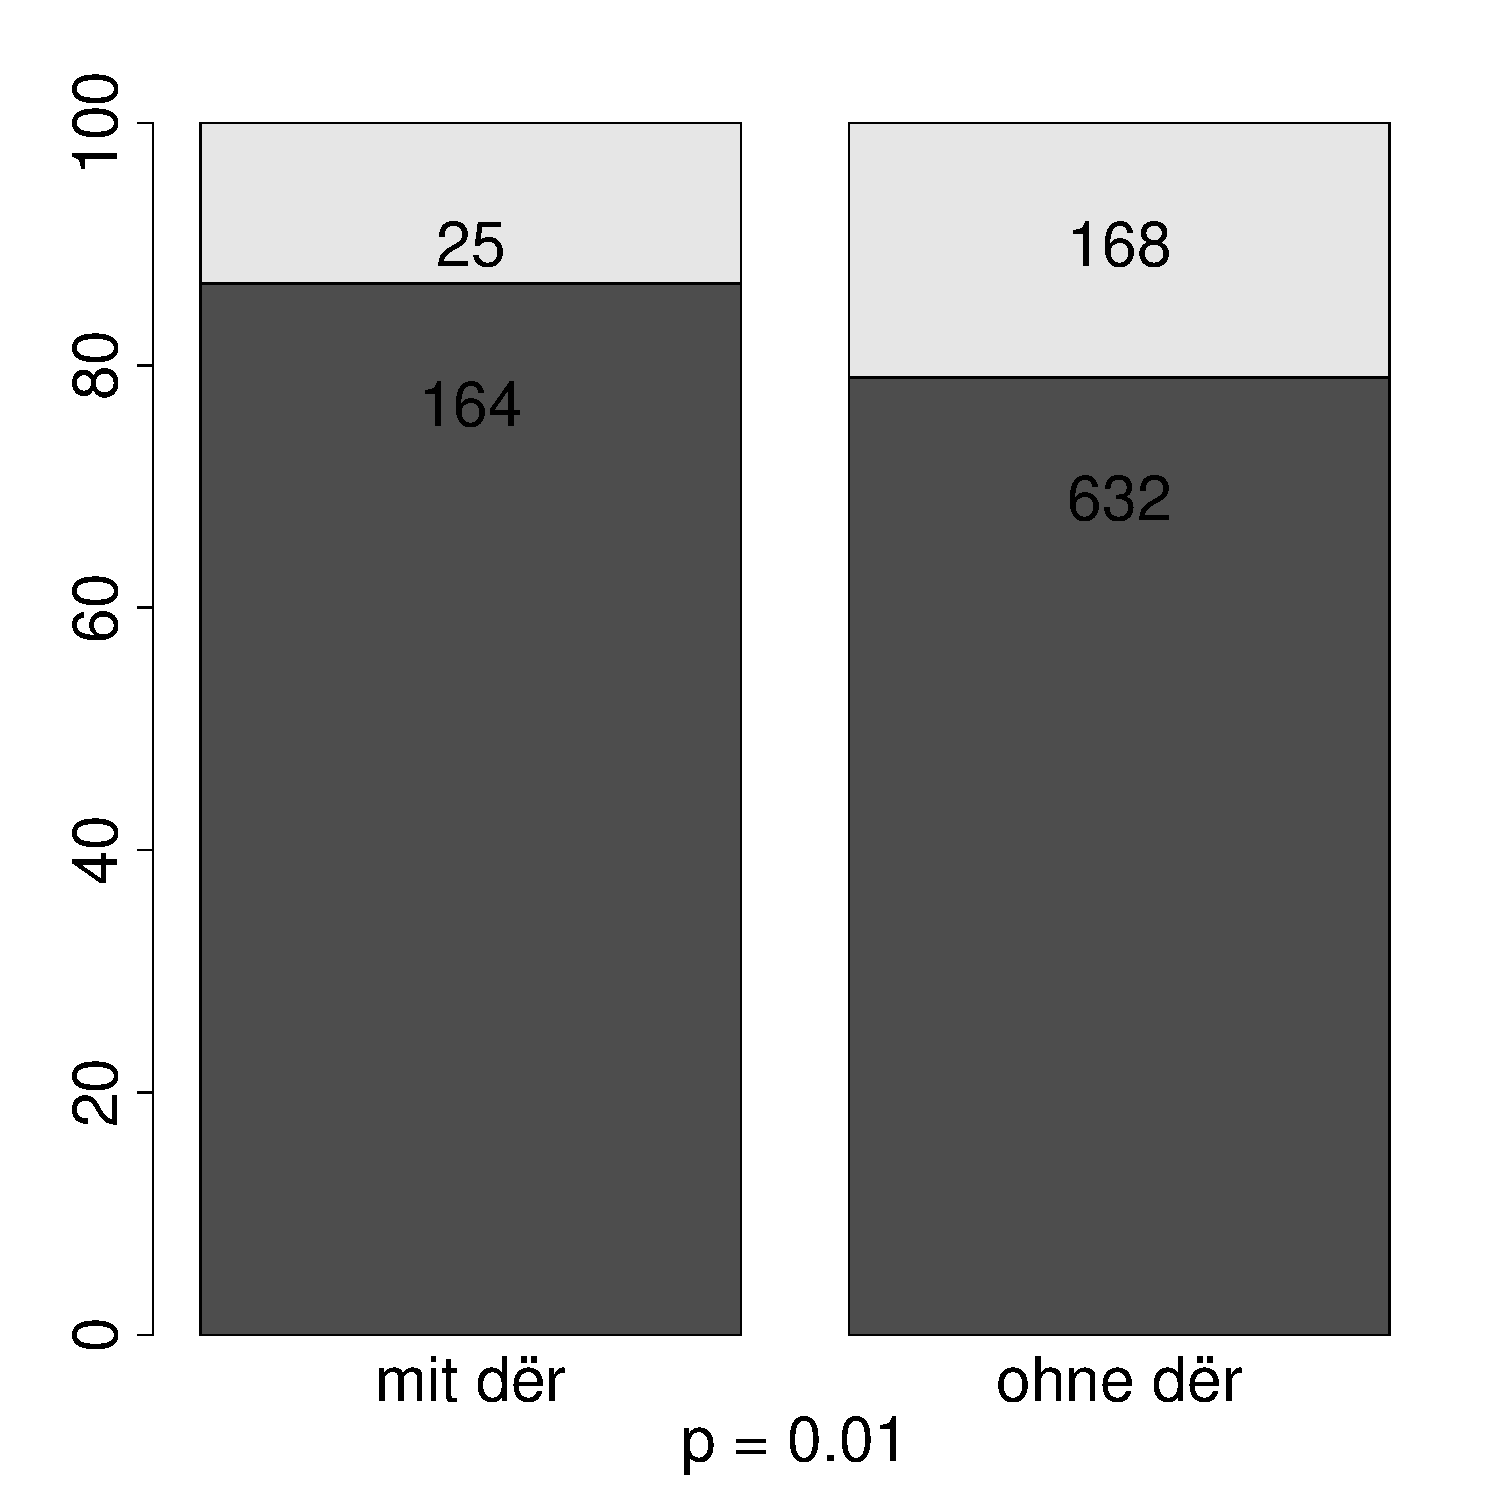
\includegraphics[height=.25\textheight]{generated/images/numerus-isidor}
\caption {Isidor}
\end{subfigure}%
\begin{subfigure}[b]{.5\linewidth}
  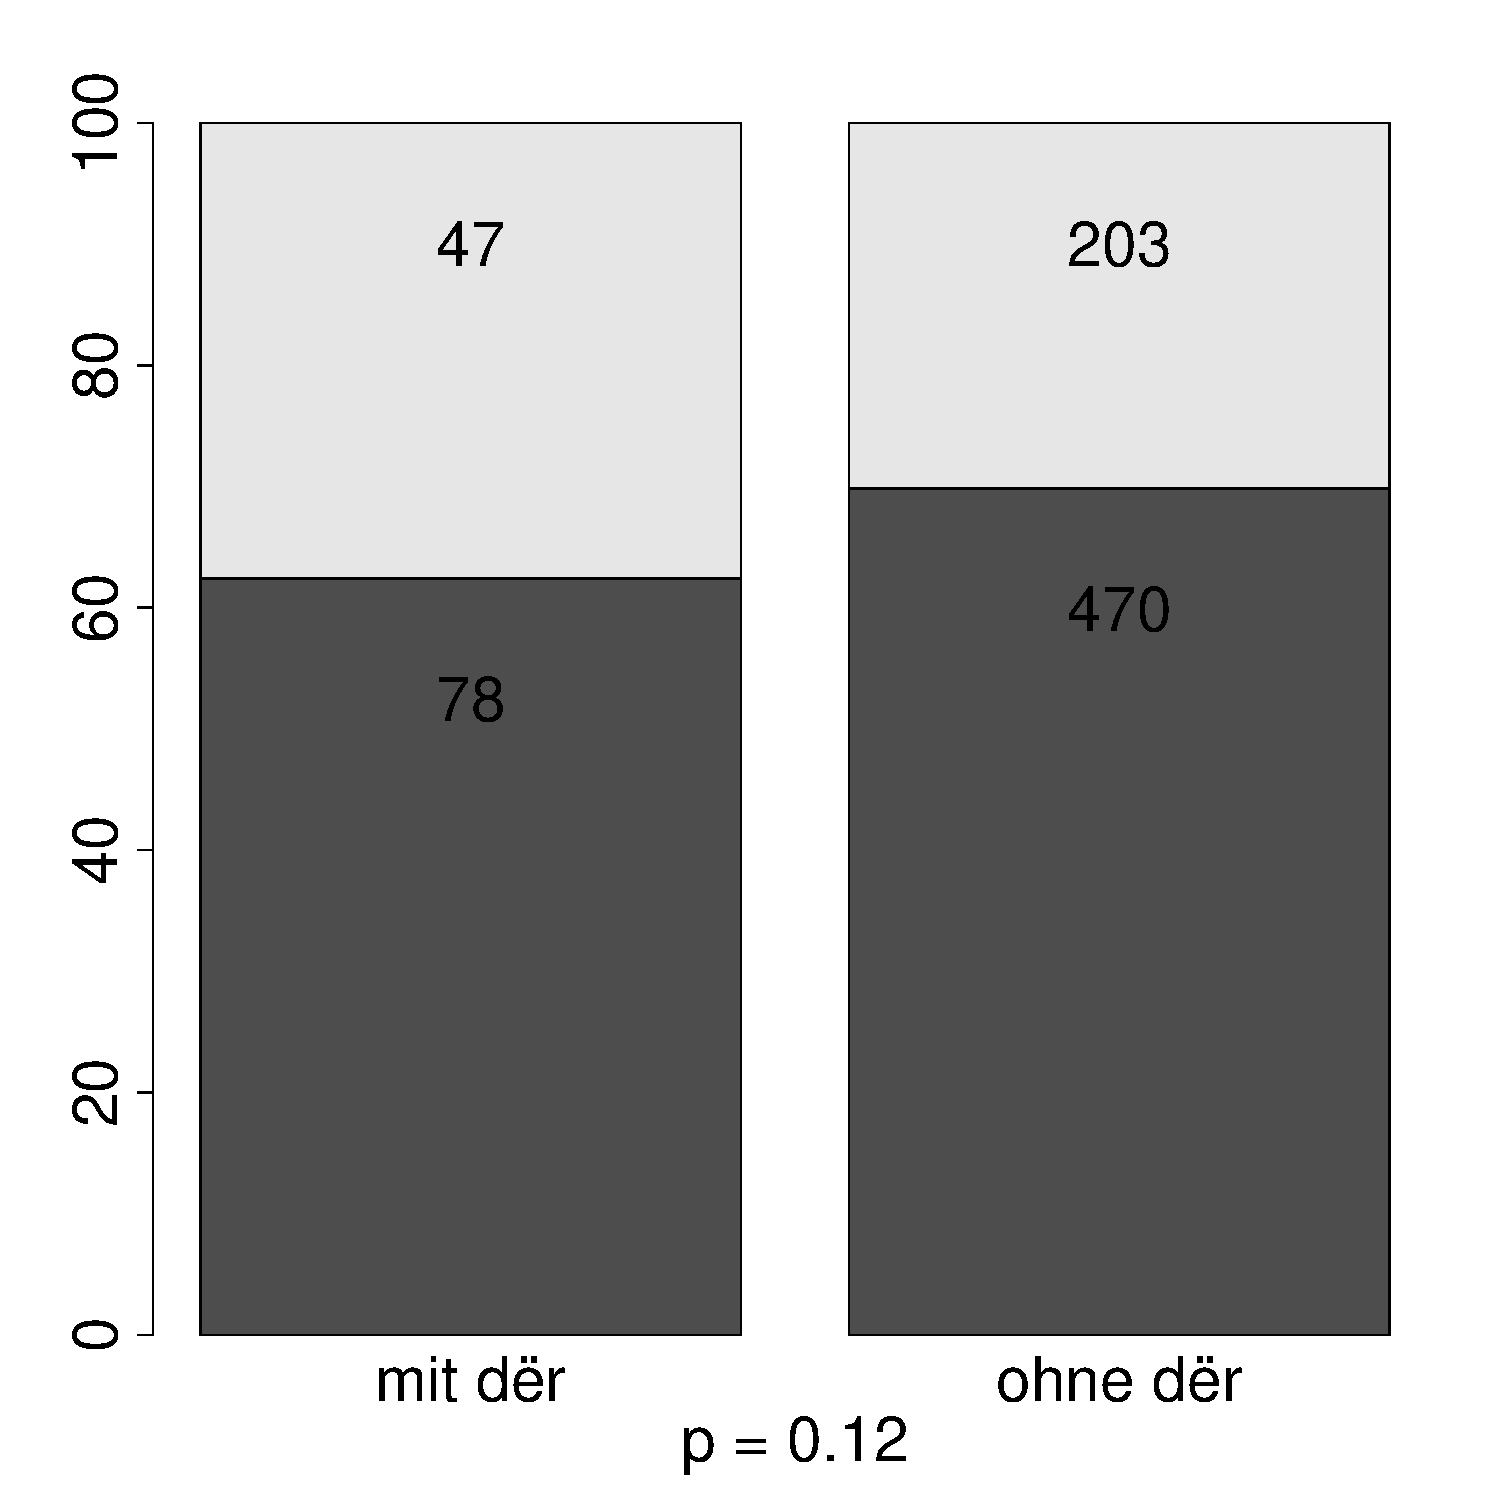
\includegraphics[height=.25\textheight]{generated/images/numerus-matt}
\caption {Monseer Matthäus}
\end{subfigure}

\begin{subfigure}[b]{.5\linewidth}
  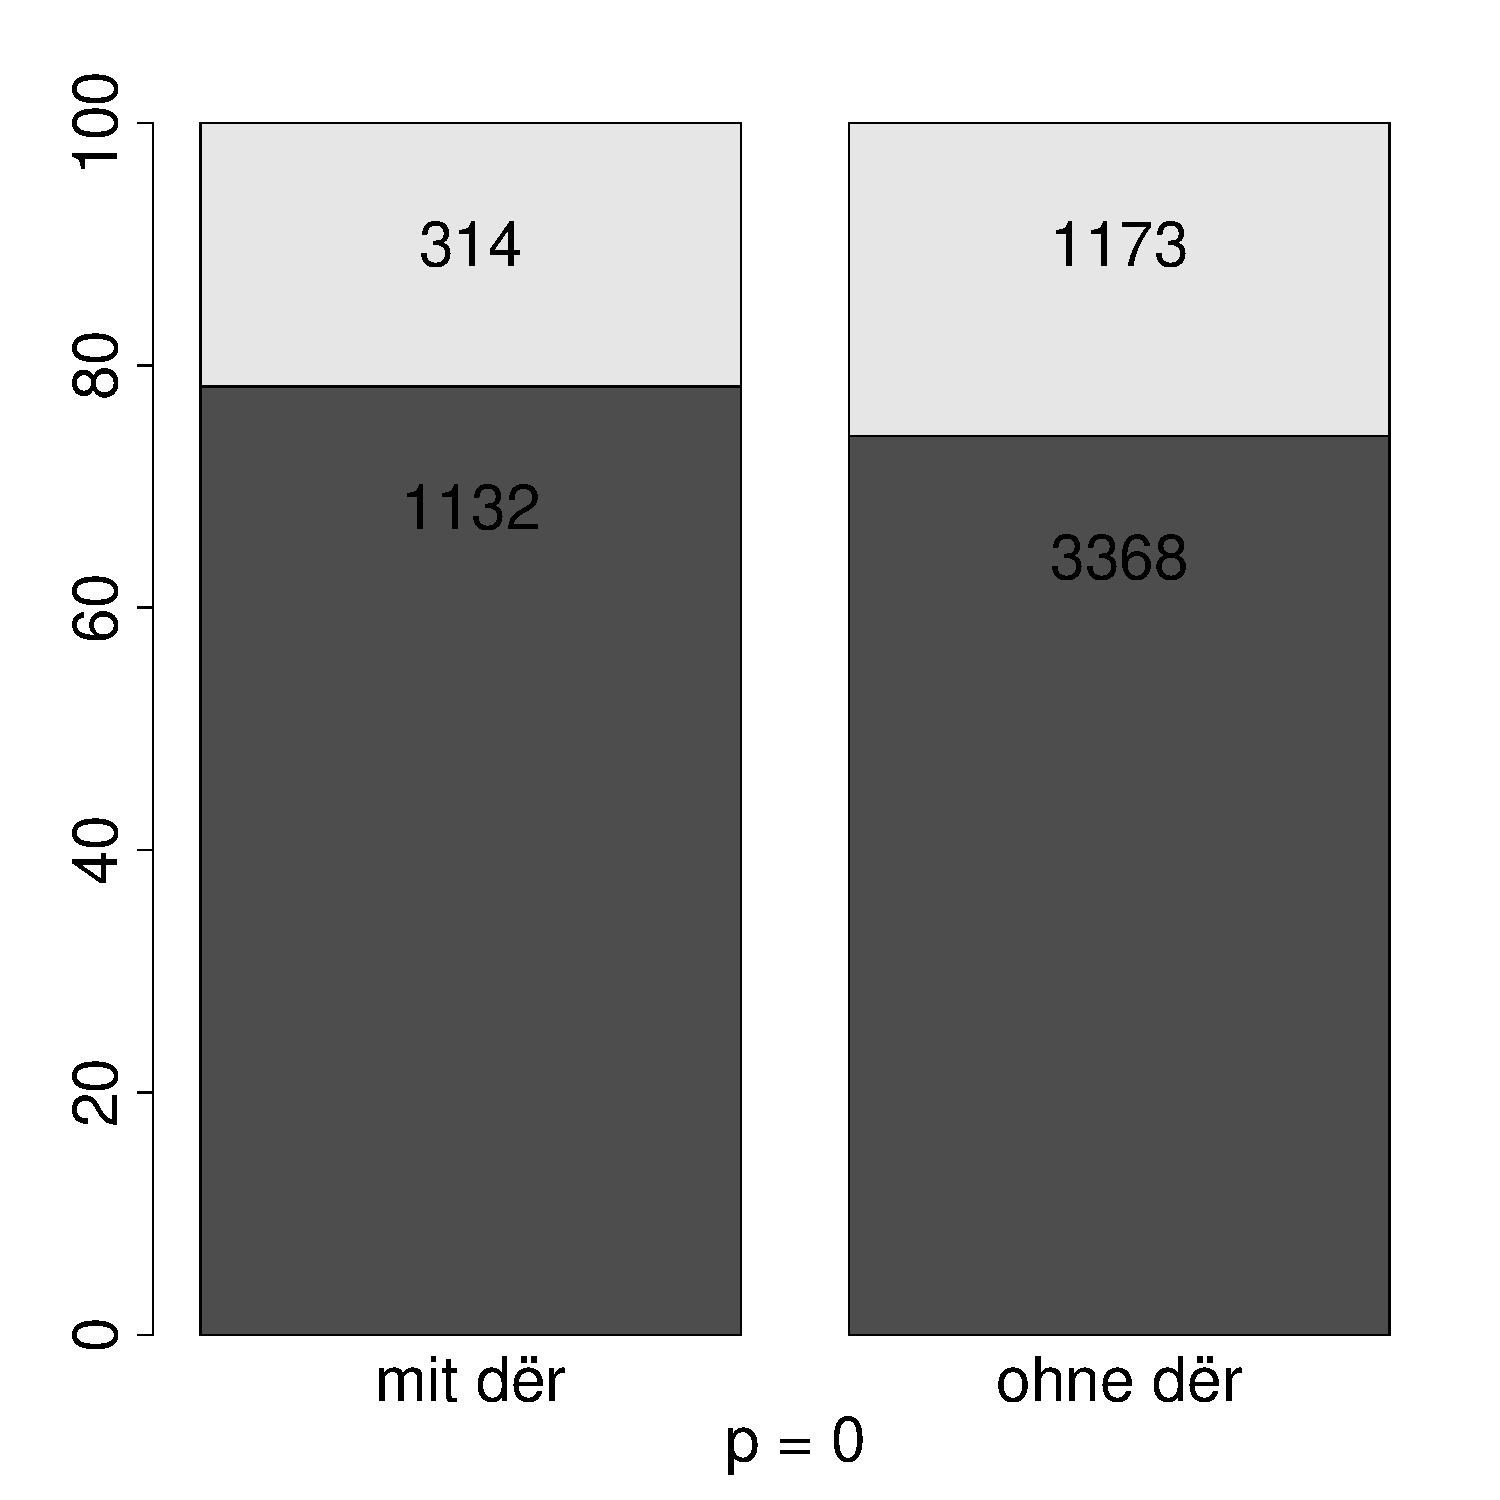
\includegraphics[height=.25\textheight]{generated/images/numerus-tatian}
\caption {Tatian}
\end{subfigure}%
\begin{subfigure}[b]{.5\linewidth}
  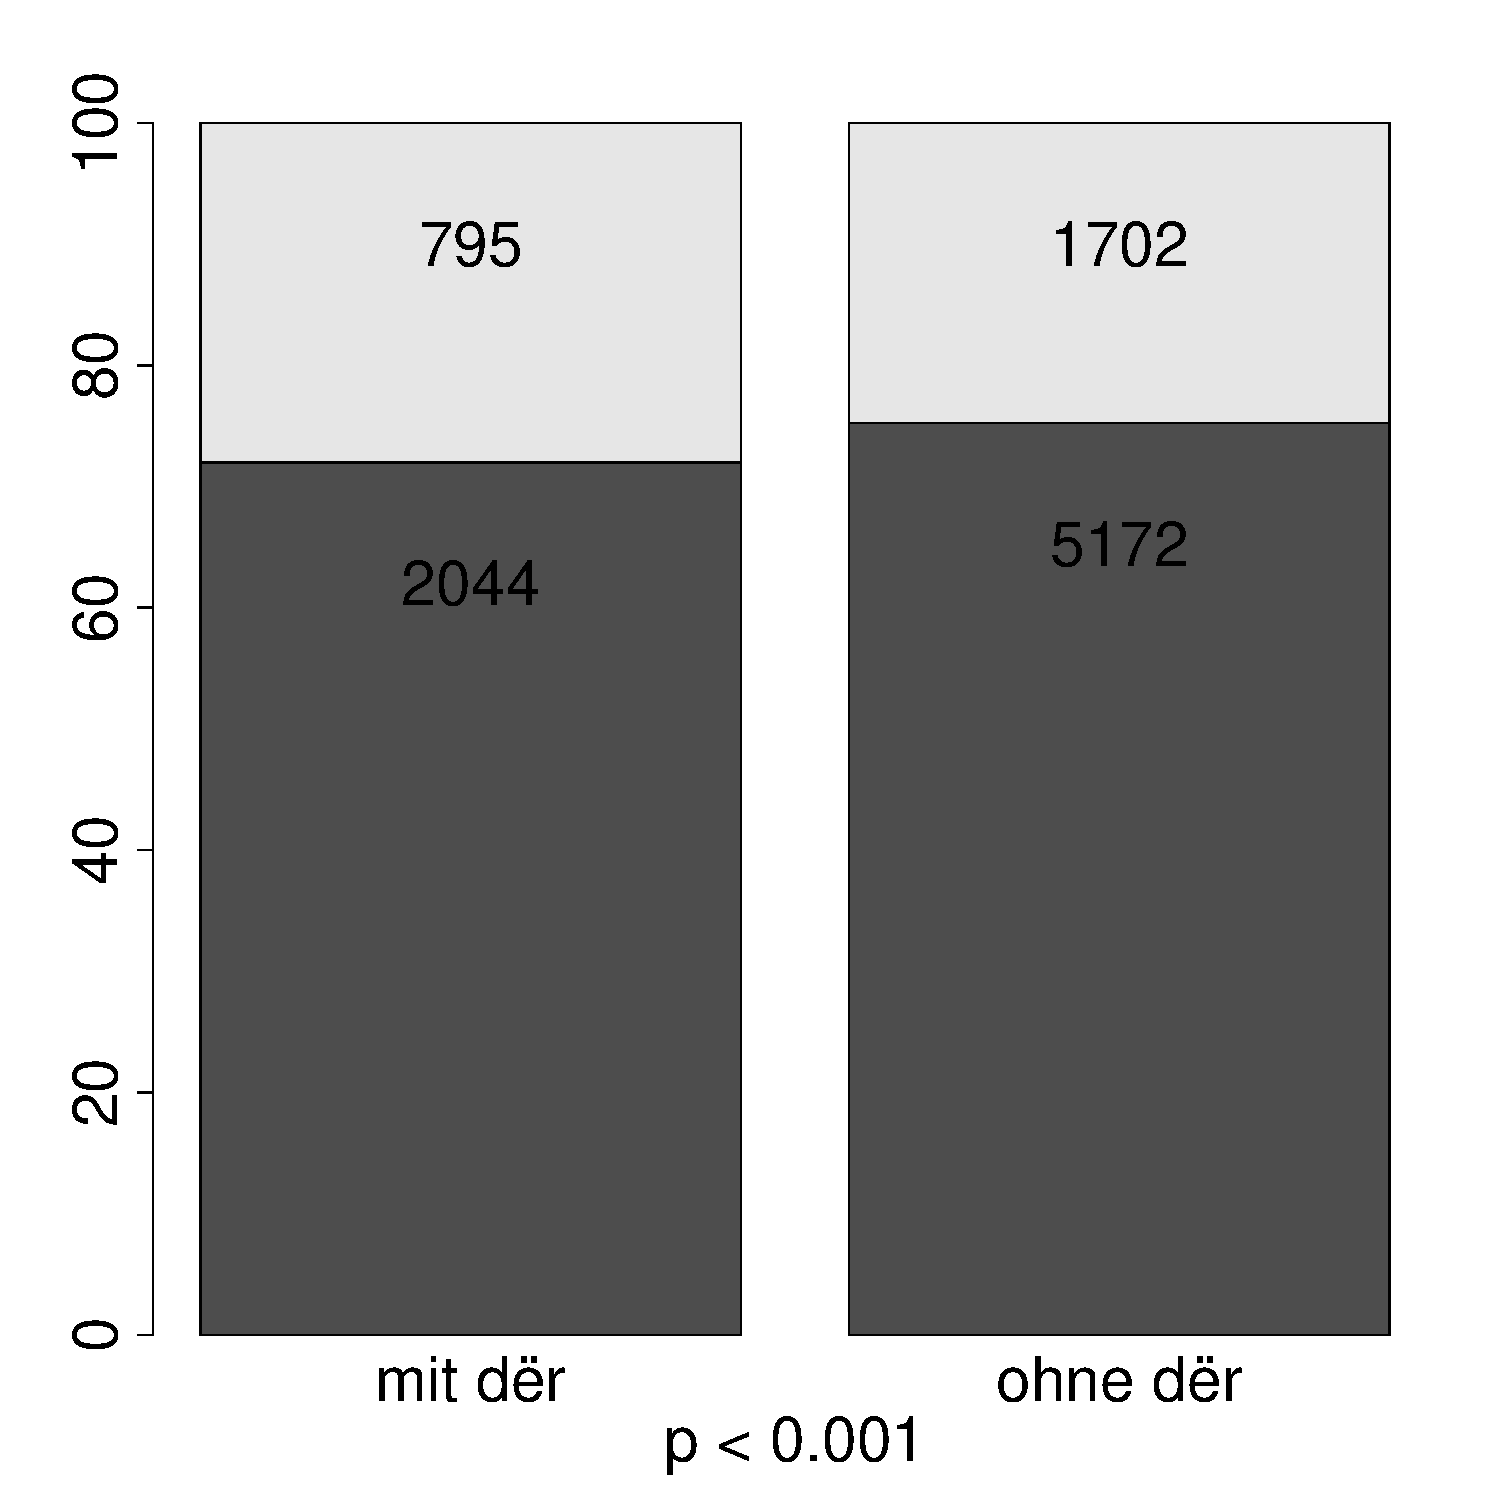
\includegraphics[height=.25\textheight]{generated/images/numerus-otfrid}
\caption {Otfrid}
\end{subfigure}

\begin{subfigure}[b]{.5\linewidth}
  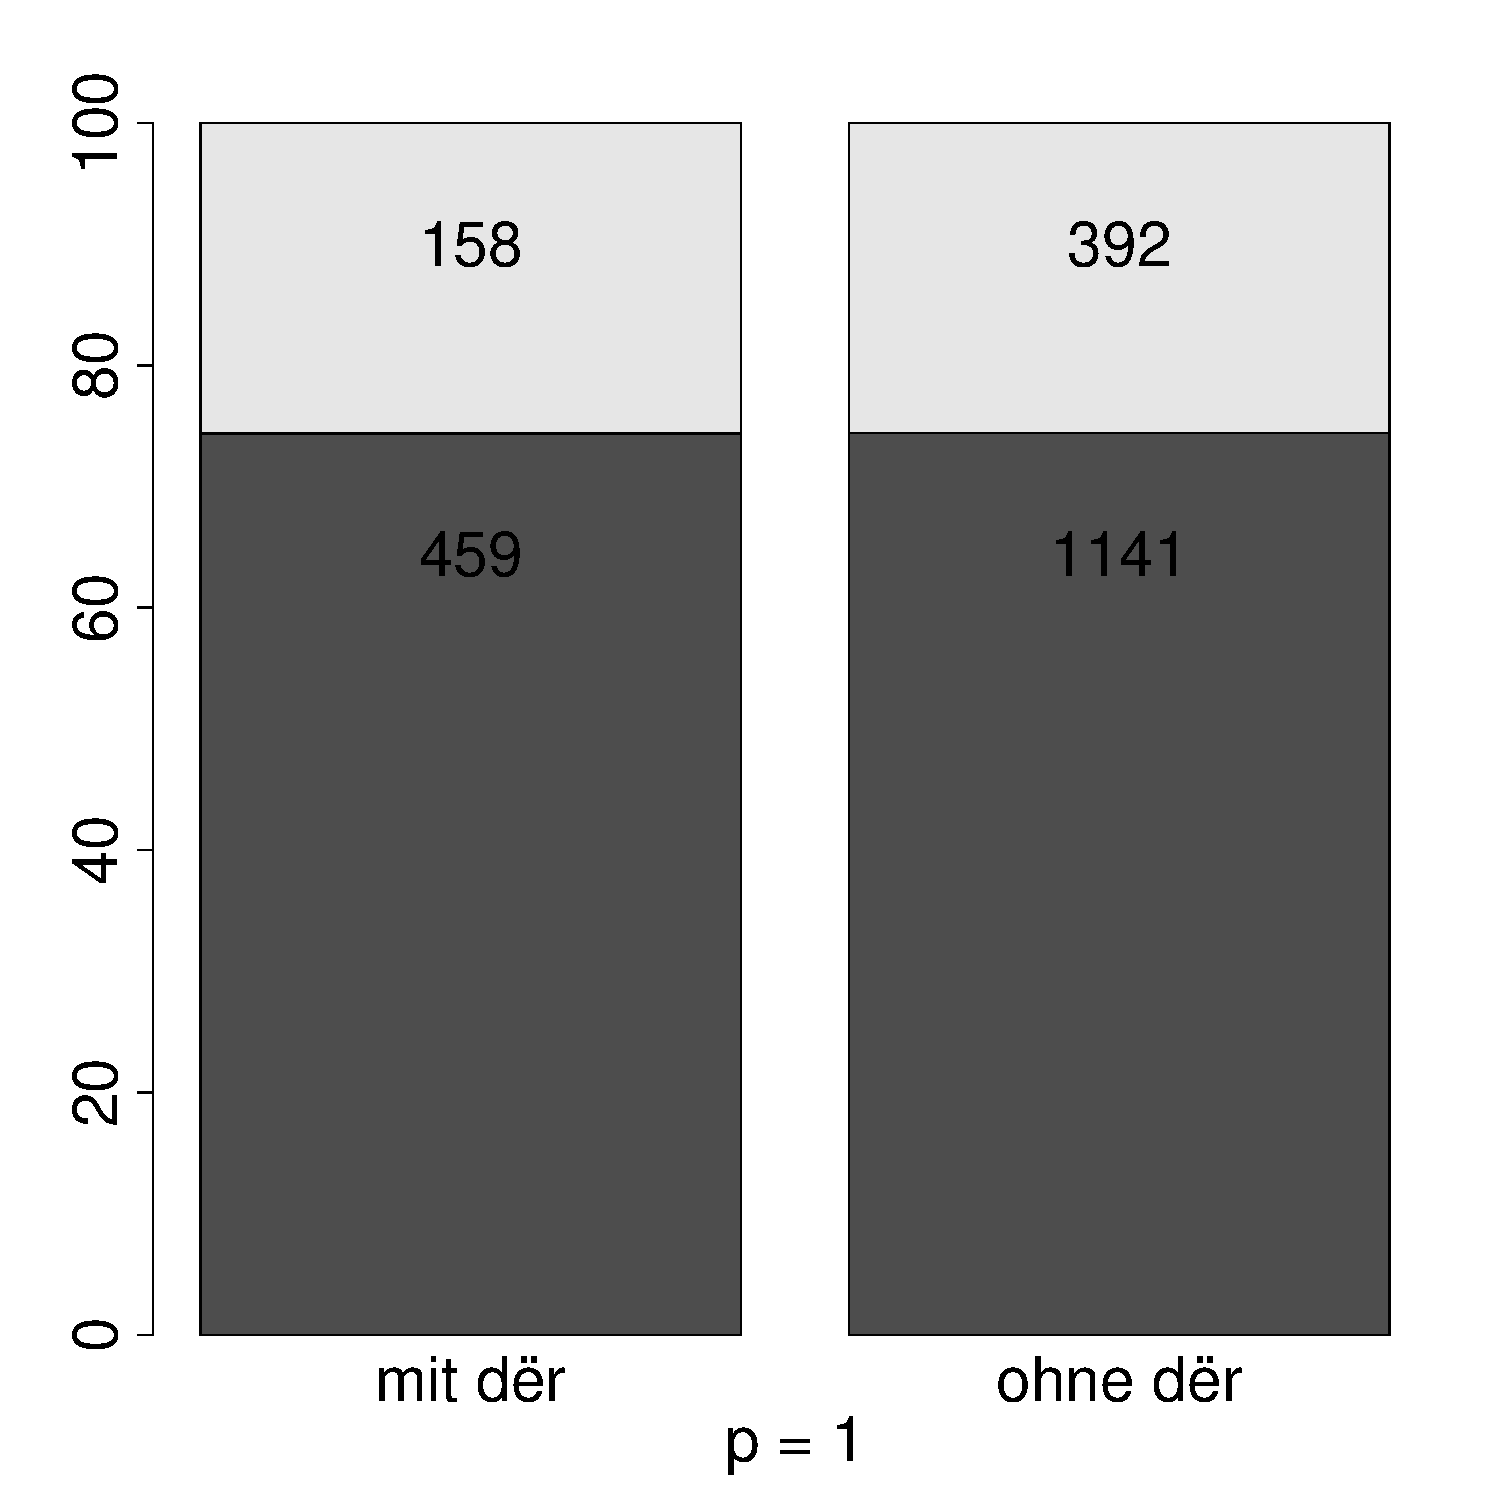
\includegraphics[height=.25\textheight]{generated/images/numerus-notker}
\caption {Notker}
\end{subfigure}%
\begin{subfigure}[b]{.5\linewidth}
  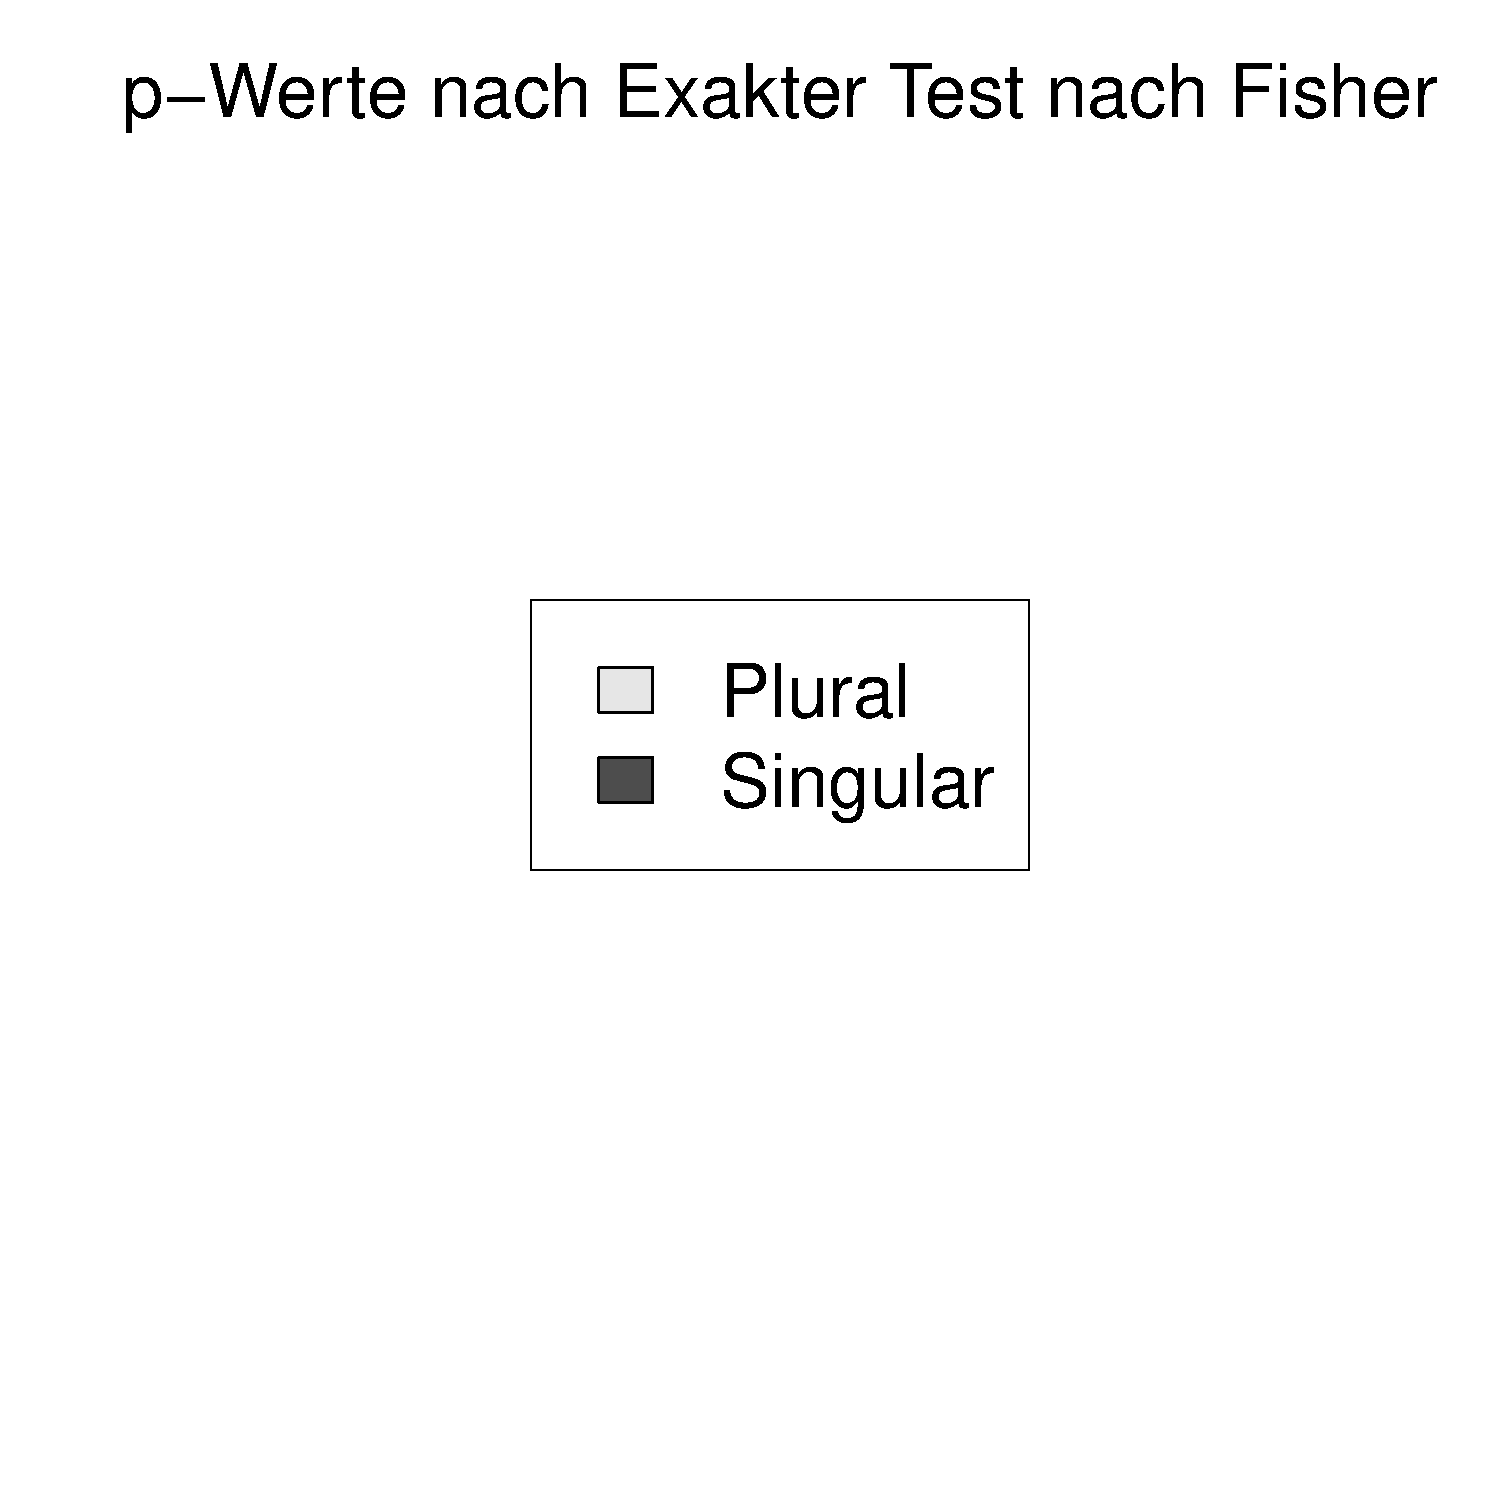
\includegraphics[height=.25\textheight]{generated/images/numerus-legende}
\end{subfigure}

\caption{Gebrauch von \object{dër} in Korrelation mit \isi{Numerus} (relative Häufigkeiten)}
\label{fig:numerus}
\end{figure}

Man sieht, dass die Belege im Singular in allen Texten deutlich in der Überzahl sind. Sie werden aber nicht zwangsläufig häufiger als erwartet mit \object{dër} determiniert. Die Unterschiede zwischen der Singular- und Pluralverteilung wurde mit Hilfe des Exakten Tests nach Fisher auf statistische Signifikanz geprüft. Im Isidor gibt es mehr Belege im Singular, die mit \object{dër} determiniert werden als im Plural. Dieser Unterschied ist signifikant ($p=0{,}01$). Die umgekehrte Tendenz im Monseer Matthäus hält dem statistischen Test nicht stand ($p=0{,}12$). Mit einem $p$-Wert,
der jeweils kleiner als $0{,}01$ ist, muss die leichte Affinität der Singularbelege zu \object{dër} im Tatian bzw. der Pluralbelege bei Otfrid dagegen als signifikant eingestuft werden. Bei Notker ist das Verhältnis ausgeglichen ($p=1$). Die Hypothese, dass Referenten im
Singular wahrscheinlicher mit \object{dër} hervorgehoben werden als plurale
Referenten, lässt sich also mit dieser Gegenüberstellung nicht verifizieren. 

Die bisherigen Ergebnisse deuten darauf hin, dass andere Faktoren den \isi{Numerus} als Individualitätsparameter \is{Individualität} überlagern: So wurde im vorhergehenden Abschnitt gezeigt, wie \isi{Massennomen} überwiegend ohne \object{dër} vorkommen, aber typischerweise im Singular stehen. Auf der anderen Seite gibt es viele belebte und konkrete Referenten, die häufig mit \object{dër} determiniert werden, aber im Plural auftreten, darunter bspw. das bei Otfrid hochfrequente \object{liut} \extrans{Volk, Leute} oder auch ganze Völkergruppen wie die Juden oder Pharisäer.


\subsection{Relevanz}\label{sec:ergeb-relevanz}

Um eine Übersicht zu erhalten, welche Lemmata \is{Lemma} in den einzelnen Texten präferiert in Kombination mit \object{dër} (sowohl in Kontakt- als auch Distanzstellung) auftreten, wurden die Daten in zwei Gruppen eingeteilt: Die eine beinhaltet alle \is{Lemma} Lemmata, deren \isi{Token} in $\geq$ 80\% aller Fälle  mit \object{dër} determiniert werden. In der anderen sind \is{Lemma} Lemmata, deren \isi{Token} in weniger als 20\%  ein \object{dër} bei sich tragen. Dargestellt sind nachfolgend jeweils die Spitzenreiter dieser Gruppen. Aus diesen Darstellungen können Rückschlüsse auf den Faktor kulturelle bzw. thematische \isi{Relevanz} gezogen werden (vgl. Abschnitt \ref{sec:relevanz}). Alle menschlichen Referenten wurden zusätzlich nach Geschlecht annotiert. Die Frage ist, ob patriarchiale Machtverhätnisse  einen Einfluss auf die \object{dër}-Setzung haben, und ob sich dies bei der Distribution von weiblichen und männlichen Referenten widerspiegelt. Die Ergebnisse hierzu werden nachfolgend in die Diskussion der Frequenzlisten eingepflegt.\footnote{Referenten, bei denen das Geschlecht unklar ist, etwa bei \object{Bürgern}, wurden nicht mit aufgenommen.} Was die nachfolgenden Daten nicht zeigen, sind konkrete Gebrauchskontexte: Ob die Belege hinter den Zahlen z.B. in anaphorische \is{anaphorisch} oder generische \is{generisch} Kontexte eingebettet sind, müsste in zukünftigen Studien überprüft werden. \footnote{Die Kategorie \object{übermenschlich}, die im Rahmen der Belebtheitsannotation \is{Belebtheit}\is{Annotation}gekennzeichnet wurde, enthält fast ausschließlich unikale Referenten (\object{Gott, der heilige Geist, der Teufel, der Heiland}). Sie wurden bereits in Abschnitt \ref{sec:ergeb-monosem} diskutiert und werden daher an dieser Stelle nicht weiter besprochen.} 

In Tabelle~\ref {tab:lemma.mit.Isidor} sind zunächst die Top-5-Lemmata \is{Lemma}  aufgeführt, die im Isidor, also dem ältesten Text, in der Mehrheit mit \object{dër} vorkommen. 

%\subsubsection{Isidor}
%Isidor mit
\inputtable{generated/tables/lemma.top10.mit-Isidor.bearbeitet}{Lemmaliste-Top-5 mit \object{dër} in $\geq$ 80\% der Belege (Isidor) }{tab:lemma.mit.Isidor}

Man sieht, dass die Liste fast ausschließlich aus biblischen Figuren besteht -- mit \object{burg} ist Jerusalem gemeint und die \object{magad} referiert immer auf die Jungfrau Maria. Interessanterweise werden andere weibliche Referenten (\object{muoter}, \object{tohter}) nicht mit \object{dër} determiniert (insgesamt wird nur auf fünf Frauen mit Appellativa \is{Gattungsname} referiert), was als Zeichen für den Einfluss der religiösen \isi{Relevanz} gewertet werden kann. 
Die nachfolgende Tabelle nimmt die umgekehrte Perspektive ein: Bei welchen Lemmata \is{Lemma} dominiert im Text die artikellose Form? Auch hier sind es biblische Referenten. Belege mit \object{truhtin} erscheinen häufig im \isi{Vokativ}, was die \object{dër}-Resistenz erklären kann. Alle anderen sind monoreferent und/oder typische Kandidaten für generische \is{generisch} Kontexte.

%Isidor ohne
\inputtable{generated/tables/lemma.top10.ohne-Isidor.bearbeitet}{Lemmaliste-Top-5 mit \object{dër} in $<20\%$ der Belege (Isidor)}{tab:lemma.ohne.Isidor}

%\subsubsection{Monseer Matthäus}

Im Monseer Matthäus sind es gesellschaftlich wichtige Referenten, die mit hoher Tokenfrequenz auftreten und mit \object{dër} determiniert werden (\object{ewawart, herizoho, herizo}), s. Tabelle~\ref{tab:lemma.mit.Matt}. Mit \object{managi} ist die Schar gemeint, die den Taten Jesus beiwohnt. Wird mit \object{diota} hingegen auf eine abstraktere und größere Menschenmenge Bezug genommen, so bleiben diese undeterminiert (vgl. Tabelle~\ref{tab:lemma.ohne.Matt}), was dafür spricht, dass hier der Faktor \isi{Individualität} zum Tragen kommt. Ähnlich wie im Isidor sind die übrigen Nomina ohne \object{dër} allerdings ebenfalls textuell  oder kulturell  relevant \is{Relevanz} (etwa \object{sun} oder \object{truhtin}).  Dass sie zur Gruppe der undeterminierten \isi{Token} gehören, hat wahrscheinlich mit ihrer Monoreferenz zu tun. 

% Matthäus mit
  \begin{table}
      \resizebox{\textwidth}{!}{% latex table generated in R 3.2.3 by xtable 1.8-2 package
% Mon Dec  3 19:12:23 2018
\begin{tabular}{rllr>{\raggedleft\arraybackslash}p{1.5cm}>{\raggedleft\arraybackslash}p{1.5cm}}
  \hline
\textbf{Rang} & \textbf{Lemma} & \textbf{Übersetzung} & \textbf{Freq.} & \textbf{Freq. mit \object{dër}} & \textbf{Rel. Anteil} \\
  \hline
1 & ewawart & Hohepriester &   7 &   7 & 1.00 \\ 
  2 & herizoho & Heerführer, Statthalter &   4 &   4 & 1.00 \\ 
  3 & heristo & Höchster, Erster &   3 &   3 & 1.00 \\ 
  4 & dorn & Dorn(strauch) &   2 &   2 & 1.00 \\ 
  5 & managi & Menge, Schar &   2 &   2 & 1.00 \\ 
   \hline
\end{tabular}
}
      \caption{Lemmaliste-Top-5 mit \object{dër} in $\geq$ 80\% der Belege (Monseer Matthäus)\label{tab:lemma.mit.Matt}}
  \end{table}
% Matthäus ohne
\inputtable{generated/tables/lemma.top10.ohne-Monsee.bearbeitet}{Lemmaliste-Top-5 mit \object{dër} in $<20\%$ der Belege (Monseer Matthäus)}{tab:lemma.ohne.Matt}

Weibliche Referenten werden selten, aber verhältnismäßig gleich häufig mit einer \object{dër}-Phrase \is{Phrase} zum Ausdruck gebracht wie männliche (3 \object{dër}-Phrasen \is{Phrase} stehen 15 Belegen ohne \object{dër} gegenüber; bei den Männern ist das Verhältnis 52 zu 231). Mit den drei \object{dër}-Phrasen \is{Phrase} ist immer die Jungfrau Maria gemeint. 

%subsubsection{Tatian}

Im Tatian wird die Präferenz des emergierenden Artikels auf männliche und ranghohe Referenten  sichtbar, s. Tabelle~\ref{tab:lemma.ohne.Tatian}. Hinzu kommt, dass bei \object{heilant}, \object{keisar} und \object{graf} meist auch ohne den spezifischen Kontext deutlich ist, welcher Referent gemeint ist \is{Semantische Definita} (=\,semantische Definitheit).

% Tatian mit 
\inputtable{generated/tables/lemma.top10.mit-Tatian.bearbeitet}{Lemmaliste-Top-5 mit \object{dër} in $\geq 80\%$ der Belege (Tatian) }{tab:lemma.mit.Tatian}
%Tatian ohne
\inputtable{generated/tables/lemma.top10.ohne-Tatian.bearbeitet}{Lemmaliste-Top-5 mit \object{dër} in $<20\%$ der Belege (Tatian)}{tab:lemma.ohne.Tatian}

Vergleicht man den Anteil der \object{dër}-Phrasen \is{Phrase} zwischen männlichen und weiblichen Referenten, zeigt sich ein signifikanter Unterschied ($p=0{,}001$ nach dem Exakten Test nach Fisher) in Richtung der männlichen Referenten mit \object{dër}, vgl. Tabelle~\ref{tab:genus-tatian}. 


\begin{table}
\centering
\begin{tabular}{lrr}
\lsptoprule
{Geschlecht}              & {mit \object{dër}} & {ohne \object{dër}} \\ \midrule
Männlich           & 28,0\% & 72,0\%    \\
Weiblich		 & 15,7\%  & 84,3\%     \\ \lspbottomrule
\end{tabular}
\caption{Geschlecht und \object{dër}-Setzung im Tatian ($n = 1725$)}
\label{tab:genus-tatian}
\end{table}

%\subsubsection{Otfrid}

Bei Otfrid lässt die hohe Tokenzahl von determinierten \object{dër}-Phrasen \is{Phrase} bei \object{grab} darauf schließen, dass hier thematische \isi{Relevanz} vorliegt: Das Grab als Ort der Auferstehung von Jesus ist in vielen Textstellen zentral und für den Zuhörer \is{Relevanz} relevant.  Das unspezifische \is{Spezifizität} \object{wiht}, das auch als Negationsverstärker dient, wird nie determiniert.  

%Otfrid mit
\inputtable{generated/tables/lemma.top10.mit-Otfrid.bearbeitet}{Lemmaliste-Top-5 mit \object{dër} in $\geq 80\%$ der Belege (Otfrid)}{tab:lemma.mit.Otfrid}
%Otfrid ohne
\inputtable{generated/tables/lemma.top10.ohne-Otfrid.bearbeitet}{Lemmaliste-Top-5 mit \object{dër} in $<20\%$ der Belege (Otfrid)}{tab:lemma.ohne.Otfrid}

Interessanterweise werden bei Otfrid weibliche Referenten eher determiniert als männliche, vgl. Tabelle~\ref{tab:genus-otfrid}. Der Unterschied ist signifikant ($p=0{,}003$ nach dem Exakten Test nach Fisher).

\begin{table}
\centering
\begin{tabular}{lrr}
\lsptoprule
{Geschlecht}              & {mit \object{dër}} & {ohne \object{dër}} \\ \midrule
Männlich           & 28,2\% & 71,8\%    \\
Weiblich		 & 38,4\%  & 61,6\%     \\ \lspbottomrule
\end{tabular}
\caption{Geschlecht und \object{dër}-Setzung bei Otfrid (n = 1883)}
\label{tab:genus-otfrid}
\end{table}

Bei Notker lässt sich aus der Übersicht der Lemmata kein Einfluss von \isi{Relevanz} ableiten. In Bezug auf das Geschlecht kommen hier die männlichen Referenten verhältnismäßig häufiger mit \object{dër} vor; der Unterschied ist signifikant ($p=0{,}002$ nach dem Exakten Test nach Fisher).


%\subsubsection{Notker}

% Notker mit
\begin{table}
  % latex table generated in R 3.2.3 by xtable 1.8-2 package
% Mon Dec  3 19:12:28 2018
\begin{tabular}{rllr>{\raggedleft\arraybackslash}p{1.5cm}>{\raggedleft\arraybackslash}p{1.5cm}}
  \lsptoprule
\textbf{Rang} & \textbf{Lemma} & \textbf{Übersetzung} & \textbf{Freq.} & \textbf{Freq. mit \object{dër}} & \textbf{Rel. Anteil} \\
  \midrule
1 & hertuom & Herrschaft, Senat &   6 &   6 & 1.00 \\ 
  2 & keisar & Kaiser &   6 &   5 & 0.83 \\ 
  3 & lihhamo & Körper, Leib &   5 &   4 & 0.80 \\ 
  4 & finstari & Finsternis &   4 &   4 & 1.00 \\ 
  5 & heroti & Obrigkeit, Senat &   4 &   4 & 1.00 \\ 
   \lspbottomrule
\end{tabular}

  \caption{Lemmaliste-Top-5 mit \object{dër} in $\geq$  80\% der Belege (Notker)\label{tab:lemma.mit.Notker}}
\end{table}

% Notker ohne
\begin{table}
  % latex table generated in R 3.2.3 by xtable 1.8-2 package
% Mon Dec  3 19:12:30 2018
\begin{tabular}{rllrrr}
  \lsptoprule
{Rang} & {Lemma} & {Übersetzung} & {Freq.} & {Freq. mit \object{dër}} & {Rel. Anteil} \\
  \midrule
1 & got & Gott &  28 &   0 & 0.00 \\ 
  2 & guot & Gut, Besitz &  24 &   2 & 0.08 \\ 
  3 & giwalt & Gewalt &  21 &   4 & 0.19 \\ 
  4 & rëht & Recht &  21 &   1 & 0.05 \\ 
  5 & situ & Sitte, Gewohnheit &  19 &   1 & 0.05 \\ 
   \lspbottomrule
\end{tabular}

  \caption{Lemmaliste-Top-5 mit \object{dër} in $<20\%$ der Belege (Notker)\label{tab:lemma.ohne.Notker}}
\end{table}

\begin{table}
\centering
\begin{tabular}{lrr}
\lsptoprule
{Geschlecht}              & {mit \object{dër}} & {ohne \object{dër}} \\ \midrule
Männlich           & 32,7\% & 67,3\%    \\
Weiblich		 & 10,7\%  & 89,3\%     \\ \lspbottomrule
\end{tabular}
\caption{Geschlecht und \object{dër}-Setzung bei Notker (n = 187)}
\label{tab:genus-notker}
\end{table}

\subsection{Semantische Rollen}\label{sec:ergeb-partizipanten}\largerpage

% table "präpositionen" von Hand basiert auf Skript "n-gramme" nach Präp
%% latex table generated in R 3.2.2 by xtable 1.8-2 package
% Sat Jul  2 17:20:56 2016
\begin{table}[ht]
\centering
\begin{tabular}{rr}
  \lsptoprule
 & V1 \\ 
  \midrule
NA & 110 \\ 
  DDA &  86 \\ 
  NE &  54 \\ 
  DPOS &  44 \\ 
  PPER &  32 \\ 
  DDS &  21 \\ 
  DI &  14 \\ 
  ADJ &   9 \\ 
  NEO &   8 \\ 
  DDSREL &   6 \\ 
   \lspbottomrule
\end{tabular}
\caption{Welche Wortarten folgen auf eine Präposition?  (Isidor)} 
\end{table}

%\input{generated/tables/pps-monsee}
%% latex table generated in R 3.2.2 by xtable 1.8-2 package
% Sat Jul  2 17:20:55 2016
\begin{table}[ht]
\centering
\begin{tabular}{rr}
  \hline
 & V1 \\ 
  \hline
NA & 817 \\ 
  PPER & 527 \\ 
  DDA & 481 \\ 
  DPOS & 276 \\ 
  NE & 103 \\ 
  NEO &  93 \\ 
  DDS &  54 \\ 
  DI &  53 \\ 
  ADJ &  52 \\ 
  DD &  44 \\ 
   \hline
\end{tabular}
\caption{Welche Wortarten folgen auf eine Präposition?  (Tatian)} 
\end{table}

%\input{generated/tables/pps-otfrid}
%\input{generated/tables/pps-notker}

Wie in Abschnitt \ref{sec:partizipanten} dargelegt wurde, ist zu erwarten, dass neben einem hohen Belebtheitsgrad \is{Belebtheit} auch der Faktor \isi{Agentivität} die \object{dër}-Setzung begünstigt. Um den Einfluss dieser Variable zu überprüfen, wurden die zufällig ausgewählten 100 NPs, die auch den Analysen der Definitheitskontexte \is{Definitheitskontext} zugrunde liegen (s. Abschnitt \ref{sec:ergeb-defkontexte}), in zwei Gruppen eingeteilt: eindeutige Agens-Belege \is{Agentivität} und Nicht-Agens-Belege. Wie die nachfolgenden Tabellen zeigen, tendiert  die \is{Agentivität} Agens-Grup\-pe in allen Texten stärker zur \object{dër}-Setzung. Im Isidor ist dieser Unterschied (nach dem Exakten Test nach Fisher) nicht signifikant ($p=0{,}75$), im Tatian und bei Otfrid hingegen schon ($p=0{,}02$, $p=0{,}002$).

\begin{table}
\centering
\begin{tabular}{lrr}
\lsptoprule
{Semantische Rolle}              & {mit \object{dër}} & {ohne \object{dër}} \\ \midrule
Agens           & 4  & 18     \\
Nicht-Agens		 & 12  & 66     \\ \lspbottomrule
\end{tabular}
\caption{Agentivität und \object{dër}-Setzung im Isidor}
\label{tab:rollen-isidor}
\end{table}

\begin{table}
\centering
\begin{tabular}{lrr}
\lsptoprule
{Semantische Rolle}              & {mit \object{dër}} & {ohne \object{dër}} \\ \midrule
Agens           & 9  & 9     \\
Nicht-Agens		 & 18  & 64     \\ \lspbottomrule
\end{tabular}
\caption{Agentivität und \object{dër}-Setzung im Tatian}
\label{tab:rollen-tatian}
\end{table}

\begin{table}
\centering
\begin{tabular}{lrr}
\lsptoprule
{Semantische Rolle}              & {mit \object{dër}} & {ohne \object{dër}} \\ \midrule
Agens           & 7  & 3     \\
Nicht-Agens		 & 17  & 73     \\ \lspbottomrule
\end{tabular}
\caption{Agentivität und \object{dër}-Setzung bei Otfrid}
\label{tab:rollen-otfrid}
\end{table}

\begin{sloppypar}
Im Isidor und Tatian denotieren fast alle Agens-Belege \is{Agentivität} in der \object{dër}-Gruppe menschliche (z.B. \object{forasago} \extrans{Prophet}, \object{buohhari} \extrans{Schriftgelehrter}) oder übermenschliche (z.B. \object{heilant} \extrans{Heiland}) Referenten. Ein Ausnahme ist das \isi{Subjekt} im Satz \object{Dhiu selba maneghiu chinomideo araughit dhazs meghiniga chiruni dhera dhrinissa} \extrans{Dieselbe Menge der Bezeichnung offenbart das machtvolle Geheimnis der Dreieinigkeit} (I 4,5). Bei Otfrid sind von den sieben Agensbelegen \is{Agentivität} mit \object{dër} zwei nicht-menschlich, einmal das \object{Los} als \isi{Subjekt} des Verbs \object{richten} (\object{ther lóz ther ríhtit unsih ál}, O IV,28) und einmal das \object{Gesetz}, das allen Leuten gebietet (\object{wio ther wízzod thuruh nót alten líutin gibot?}, O II,18). 
\end{sloppypar}

In einem zweiten Schritt wurden Präpositionalphrasen \is{Präpositionalphase (PP)} in den Blick genommen, da davon ausgegangen werden kann, dass diese primär zum Ausdruck von modifizierenden Angaben (etwa lokale, temporale oder zeitliche Verortung) genutzt werden und daher am weitesten vom prototypischen Agenspol entfernt sind. Sie sollten deswegen eine gewisse Resistenz gegenüber \object{dër} aufweisen. Die Gegenüberstellung in Tabelle~\ref{table:präpositionen} bestätigt diese Hypothese. Die Daten basieren auf einer Bigramm-Auswertung \is{Bigramm} des gesamten \isi{Korpus}: Es wurde ausgezählt, wie häufig ein \object{dër} auf ein \isi{Token} folgt, das als Präposition annotiert ist. 

\begin{table}
\centering
\begin{tabular}{lrrrrr}
\lsptoprule
            {Text} & \multicolumn{2}{c}{{Präp\,+\,N}} & \multicolumn{2}{c}{{Präp\,+\,\object{dër}\,+\,N}} &       {Summe} \\\cmidrule(lr){2-3}\cmidrule(lr){4-5}
            & {Freq.}        &{\%}          & {Freq.}           &{\%}              &  \\
       \midrule
Isidor      & 110            & 56,1        & 86                & 43,9            & 196    \\
M. Matthäus & 139            & 71,3        & 56                & 28,7            & 195    \\
Tatian      & 817            & 62,9        & 481               & 37,1            & 1298   \\
Otfrid      & 1616           & 71,2        & 653               & 28,8            & 2269   \\
Notker      & 268            & 56,2        & 209               & 43,8            & 477    \\ \lspbottomrule
\end{tabular}
\caption{[Präp\,+\,N] im Vergleich zu [Präp\,+\,\object{dër}\,+\,N]}
\label{table:präpositionen}
\end{table}

Betrachtet man nur den ältesten und jüngsten Text, ist kein diachroner Unterschied sichtbar: Sowohl Isidor als auch Notker verfügen jeweils über das gleiche Verhältnis von determinierten gegenüber undeterminierten Phrasen  (ca. 44\% zu 56\%). Der Vergleich zwischen Monseer Matthäus und Tatian und damit den beiden Texten, die am besten miteinander vergleichbar sind, weil sie sich von der Textsorte und vom Inhalt her ähneln, zeigt einen Anstieg von knapp 10\% zugunsten der Struktur [Präp\,+\,\object{dër}\,+\,N]. Dieser Anstieg relativiert sich allerdings bei Otfrid wieder.  

Wie groß der Anteil an anderen syntaktischen Funktionen unter den Präpositionalphrasen \is{Präpositionalphase (PP)} ist, die damit auch anderen semantischen Rollen \is{Semantische Rolle} entsprechen würden (etwa Präpositionalobjekte \is{Objekt} als Patiens), muss in zukünftigen Studien überprüft werden, damit weitere Korrelationen zwischen semantischer Rolle \is{Semantische Rolle} und Artikelsetzung sichtbar werden. 


\section{Struktur der Nominalphrase}\label{erg:struktur.np}

In diesem Abschnitt werden die Ergebnisse zur Struktur der Nominalphrase \is{Nominalsyntax}\is{Nominalphrase (NP)}präsentiert. In Abschnitt~\ref{sec:ergeb-np-struktur} wird der Fokus auf pränominale Strukturmöglichkeiten \is{Wortstellung}\is{Nominalsyntax}gesetzt, die sich aus den Daten ablesen lassen. Danach zeigt Abschnitt \ref{sec:ergebnisse-stellung}, wie das Häufigkeitsverhältnis von Voran- und Nachstellung bei \object{dër} und anderen Determinierern \is{Determinierer} in den Daten aussieht. In Abschnitt \ref{sec:ergeb-adjflex} wird der Frage nachgegangen, inwiefern die schwache Adjektivflexion \is{Flexion}\is{Adjektiv}eine Setzung von  \object{dër} auslöst. 

\subsection{Pränominale Strukturmöglichkeiten}\label{sec:ergeb-np-struktur}

Mithilfe der Wortartenannotion wurden Proxys \is{Proxy} definiert, die bestimmten NP-Strukturtypen \is{Nominalsyntax} entsprechen. Die Basis für die Auswahl der Strukturtypen diente die bisherige Forschung zur Struktur der NP \is{Nominalsyntax} im Althochdeutschen \parencite[vor allem][]{Oubouzar1989}. 

\begin{itemize}
\item [a)] \object{dër}\,+\,( \_\_+ )  Nomen Appellativum
\item [b)] Possessivpronomen\,+\,( \_\_+ )  Nomen Appellativum
\item [c)] Adjektiv\,+\,( \_\_+ )  Nomen Appellativum
\item [d)] Indefinites Element\,+\,( \_\_+ )   Nomen Appellativum
\item [e)] Nomen\textsubscript{Genitiv}\,+\,( \_\_+ )   Nomen Appellativum
\item [f)] Nomen\textsubscript{kein Genitiv}\,+\,( \_\_+ )   Nomen Appellativum
\end{itemize}

\noindent 
Bei den deklinierbaren Elementen wurde darauf geachtet, dass Übereinstimmung von \isi{Kasus}, \isi{Numerus} und \isi{Genus} vorliegt. Ein vorangestelltes Nomen im Genitiv entspricht in der Regel einem Attribut \is{Genitivattribut} (etwa \object{gotes sunu}). Folgt der Beleg einem Nomen im anderen \isi{Kasus}, lässt sich dies meist damit erklären, dass  der Beleg selbst als \isi{Genitivattribut} fungiert (z.B. \object{gheist druhtines}). 
 
Mit den vorliegenden Ergebnissen lässt sich für alle Texte beantworten, wie viele Appellativa \is{Gattungsname} ohne \isi{Determinierer} bzw. phraseneinleitende Elemente auftreten und wie salient \object{dër} als \isi{Determinierer} ist. Ferner können aus den Daten Rückschlüsse in Bezug auf ein mögliches  Determinierschema gemacht werden, das sich im Laufe des Althochdeutschen herausbildet (s. hierzu ausführlich die Diskussion in Kapitel \ref{bicpic}). Dargestellt werden nachfolgend jeweils die zehn häufigsten Strukturtypen; die weniger frequenten finden sich gruppiert am Ende der Tabelle unter \hervor{Andere}.  Was man an dieser Datenauswertung  nicht ablesen kann, sind  Abweichungen im Vergleich zur lateinischen Vorlage bei den bilingualen Texten. Daher wurde zusätzlich eine Stichprobe von je 100 NPs pro Text strukturell annotiert (vgl. die Beschreibung in Abschnitt \ref{sec:annotationsschritte}) und die Auswertung an den entsprechenden Stellen eingepflegt.

% Skript: NA-artikel: 4 Struktur der NP [Pos1 Pos2 N ]

%\subsubsection{Isidor}

In Tabelle~\ref{tab:np-isidor} sind die Top-10-Stukturtypen für Isidor aufgeführt, welche die Proxy-Suchabfrage \is{Proxy} hervorgebracht hat. 

\begin{table}
\centering
\begin{tabular}{clllrrl}
\lsptoprule
{\#} & {Det. 1}  & {Det. 2}  & & {Freq.}  &\%  & {Beispiel}   \\ \midrule
1        & ∅          & ∅             & \rdelim\}{11}{4mm}[\,+\,N] & 374        & 37,8  & \textit{sunu}                              \\
2        & ∅          & Nomen\textsubscript{Gen.}       && 152        & 15,4 & \textit{dauides samin}                   \\
3        & ∅          & Poss.          && 104        & 10,5 & \textit{siin grab}                        \\
4        & ∅          & \object{dër}           && 90         & 9,1  & \textit{dhen forasagun}                   \\
5        & \object{dër}         & Adj.          && 57         & 5,8 & \textit{in dhemu hebræischin chiscribe}   \\
6        & ∅          & Adj.           && 53         & 5,4  & \textit{liuzil chind}                     \\
7        & ∅          & Nomen         && 43         & 4,3  & \textit{gheist druhtines}                 \\
8        & \object{dër}         & Nomen\textsubscript{Gen.}       && 19         & 1,9 & \textit{dhiu iesses uurza}                \\
9        & \object{dër}         & \object{sëlb}         && 19         & 1,9 & \textit{dher selbo druhtin}               \\
10       & ∅          & Indef.          && 18         & 1,8  & \textit{einigan chuninc}                 \\
11       & \multicolumn{2}{c}{Andere} && 61         & 6,2 & \textit{allan mittingart, dheasa stat...} \\ \midrule
         & \multicolumn{2}{c}{Summe} && 990        & 100 &                                           \\ \lspbottomrule
\end{tabular}
\caption{Die häufigsten NP-Strukturtypen im Isidor}
\label{tab:np-isidor}
\end{table}

Auffällig ist, dass [Nomen\,+\,Nomen]-Verbindungen im Isidor mit fast 20\%\linebreak recht häufig sind, s. Strukturtyp 2 und 7. \is{Gattungsname} Appellativa, die unmittelbar mit \object{dër} determiniert werden, machen gut 9\% der Belege aus. Knapp 8\% der \object{dër}-Phrasen \is{Phrase} klammern \is{Nominalklammer} ein weiteres kongruierendes Element, meist ein \isi{Adjektiv} oder auch ein deiktisches \object{sëlb}, ein. In nur knapp 2\% der Belege kookkurriert \object{dër} mit einem \isi{Genitivattribut} (19 Fälle) und nur einmal tritt \object{dër} in Kombination mit einem \isi{Possessivum} auf (\object{fona dheru sineru uurzun}). Possessiva \is{Possessivum} nehmen mit ca. 12\% den zweiten Platz der \isi{Determinierer} ein. Das demonstrative \object{dëser} \is{Demonstrativum}kommt 16 mal vor und macht damit  knapp 2\% der \isi{Determinierer} aus. Knapp 36\% aller Nomen erscheinen ohne Phraseneinleiter oder \is{Genitivattribut} Genitivattribuierung. Nicht alle dieser Nomen sind jedoch definit:  Nimmt man die Ergebnisse der Stichprobenanalyse zum Vergleich (s. Abschnitt \ref{sec:ergeb-defkontexte}), so tragen im Isidor von 100 Belegen 17 Belege eine indefinite  \is{Indefinitheit} bzw. unspezifische \is{Spezifizität} Referenz, 19 sind monoreferentiell. Hochgerechnet lässt sich daher davon ausgehen, dass immerhin ein Drittel der Belege aufgrund ihrer Referenz"-eigenschaften aus dem Raster der potentiell determinierbaren \is{Gattungsname} Appellativa fallen. Fast 30\% (110) der blanken Nomen (Strukturtyp 1) sind in eine PP eingebettet, was ebenfalls die \object{dër}-Setzung blockieren könnte. 

Die Auswertung der zufällig ausgewählten 100 NPs im Isidor zeigt, dass potentielle Phraseneinleiter, allen voran \object{dër} und \is{Possessivum} Possessiva, in den meisten Fällen entgegen der lateinischen Vorlage gesetzt werden, s. Tabellen~\ref{tab:diff-ther-isidor} und~\ref{tab:diff-poss-isidor}. Wenn es im Lateinischen kein grammatisches Äquivalent gibt, so wird \object{dër} bzw. das \isi{Possessivum} vorangestellt. Wenn ein nachgestelltes Äquivalent existiert, präferiert der Übersetzer ebenfalls die Voranstellung.

% Stichprobe-NP-Struktur.R # 1
\begin{table}
\centering
\begin{tabular}{lrrr}
\lsptoprule
                   & \multicolumn{2}{c}{Latein} & \multirow{2}{*}{keine lat. Vorlage}\\
 \cmidrule(lr){2-3}
                   & vorangestellt & nachgestellt & \\ \midrule
Ahd. vorangestellt & 0                  & 0                 & 16                    \\
Ahd. nachgestellt  & 0                  & 0                 & 0                    \\ \lspbottomrule
\end{tabular}
\caption{Differenzbelege \is{Differenzbeleg} von \object{dër} im Isidor}
\label{tab:diff-ther-isidor}
\end{table}

\begin{table}
\centering
\begin{tabular}{lrrr}
\lsptoprule
                   & \multicolumn{2}{c}{Latein} & \multirow{2}{*}{keine lat. Vorlage}\\
 \cmidrule(lr){2-3}
                   & vorangestellt & nachgestellt & \\ \midrule
Ahd. vorangestellt & 0                  & 10                 & 1                    \\
Ahd. nachgestellt  & 0                  & 1                 & 0                    \\ \lspbottomrule
\end{tabular}
\caption{Differenzbelege \is{Differenzbeleg} der Possessiva \is{Possessivum} im Isidor}
\label{tab:diff-poss-isidor}
\end{table}

Belege mit Adjektiven \is{Adjektiv} sind seltener. Die sechs betreffenden NPs zeigen allerdings auch hier eine Tendenz zur Voranstellung -- auch entgegen der Vorlage. 

\begin{table}
\centering
\begin{tabular}{lrrr}
\lsptoprule
                   & \multicolumn{2}{c}{Latein} & \multirow{2}{*}{keine lat. Vorlage}\\
 \cmidrule(lr){2-3}
                   & vorangestellt & nachgestellt & \\ \midrule
Ahd. vorangestellt & 1                  & 2                 & 2                    \\
Ahd. nachgestellt  & 0                  & 1                 & 1                    \\ \lspbottomrule
\end{tabular}
\caption{Differenzbelege \is{Differenzbeleg} der Adjektive \is{Adjektiv} im Isidor}
\label{tab:diff-adj.-isidor}
\end{table}

%\subsubsection{Monseer Matthäus}

Tabelle~\ref{tab:np-matt} dokumentiert die zehn häufigsten Strukturtypen im Monseer Matthäus auf Basis der \is{Proxy} Proxysuche. 

\begin{table}
\begin{tabular}{clllrrl}
\lsptoprule
{\#} & {Det. 1}  & {Det. 2}  & & {Freq.}  &\%    \\ \midrule
1        & ∅           & ∅            & \rdelim\}{11}{4mm}[\,+\,N] & 391        & 49,0 \\
2        & ∅           & \object{dër}          && 88         & 11,0 \\
3        & ∅           & Poss.         && 75         & 9,4  \\
4        & ∅           & Nomen\textsubscript{Gen.}       && 69         & 8,6  \\
5        & ∅           & Adj.          && 49         & 6,1  \\
6        & ∅           & Nomen        && 36         & 4,5  \\
7        & \object{dër}           & Adj.          && 19         & 2,4  \\
8        & ∅           & \object{al}           && 13         & 1,6  \\
9        & ∅           & \object{dëse}         && 9          & 1,1  \\
10       & ∅           & Indef.        && 9          & 1,1  \\
11       & \multicolumn{2}{c}{Andere} && 40         & 5,0  \\ \midrule
         & \multicolumn{2}{c}{Summe} && 798        & 100  \\ \lspbottomrule
\end{tabular}
\caption{Die häufigsten NP-Strukturtypen im Monseer Matthäus}
\label{tab:np-matt}
\end{table}

Jede zweite \isi{Phrase} in diesem Text ist eine blanke NP. Auch hier lässt sich ein Teil der  Determiniererlosigkeit \is{Determinierer} dadurch erklären, dass auf indefinite oder monosemantische \is{Unikum} Referenten verwiesen wird. Auffällig ist, dass [Nomen\,+\,Nomen]-Bigramme \is{Bigramm} weniger häufig als im Isidor vorkommmen. Die meisten eingeleiteten Phrasentypen enthalten entweder ein \object{dër} oder ein \isi{Possessivum}. Kookkurrenzen von \object{dër} und \isi{Possessivum} sind mit $<1\%$ marginal (sie wurden unter \hervor{Andere} gefasst). Die \isi{Nominalklammer}  ist nur wenig ausgebaut: \object{dër}\,+\,Adjektivstrukturen \is{Adjektiv} machen nur knapp 2,4\% der Belege aus. Ferner zeigt eine  Bigrammauswertung \is{Bigramm} zu Strukturtyp 1 (Vergleich der Häufigkeiten von [Präposition\,+\,Nomen] mit [Nicht-Präpostion\,+\,Nomen]), dass 28\% der blanken NPs in eine PP eingebettet sind (110 von 391). 

%\subsubsection{Tatian}

Im Tatian ähnelt die Top-10-Frequenzliste der Situation im Monseer Matthäus.  Allerdings tritt [\object{dër}\,+\,N] mit mehr als 21\% deutlich häufiger auf, s. Tabelle~\ref{tab:np-tatian}.    

\begin{table}
\centering
\begin{tabular}{clllrrl}
\lsptoprule
{\#} & {Det. 1}  & {Det. 2}  & & {Freq.}  &\%   \\ \midrule
1    & ∅           & ∅            & \rdelim\}{11}{4mm}[\,+\,N] & 2625     & 43,6      \\
2    & ∅           & \object{dër}          && 1277     & 21,2      \\
3    & ∅           & Poss.         && 832      & 13,8      \\
4    & ∅           & Adj.          && 326      & 5,4       \\
5    & ∅           & Nomen\textsubscript{Gen.}       && 251      & 4,2       \\
6    & ∅           & Nomen        && 206      & 3,4       \\
7    & ∅           & \object{dëse}         && 102      & 1,7       \\
8    & \object{dër}         & Adj.          && 86       & 1,4       \\
9    & ∅           & Indef.        && 72       & 1,2       \\
10   & ∅           & \object{al}           && 44       & 0,7       \\
11   & \multicolumn{2}{c}{Andere} && 194      & 3,2       \\ \midrule
     & \multicolumn{2}{c}{Summe} && 6015     & 100       \\ \lspbottomrule
\end{tabular}
\caption{Die häufigsten NP-Strukturtypen im Tatian}
\label{tab:np-tatian}
\end{table}

Die Strukturtypen \is{Possessivum} [Possessivum\,+\,N] sowie \is{Adjektiv} [Adjektiv\,+\,N] kommen häufiger vor als [Nomen\textsubscript{Gen.}\,+\,N]. Wie in den beiden anderen Texten (Isidor und Monseer Matthäus) sind die anderen flektierenden \is{Flexion} Elemente wie das \isi{Demonstrativum} \object{dëser} oder indefinite Ausdücke für sich genommen marginal. Gruppiert man diese in die Kategorie der phraseneinleitenden Strukturtypen, so macht diese Gruppe insgesamt allerdings fast die Hälfte aller Belege aus. Die undeterminierten NPs liegen bei knapp 44\%. Sie reduziert sich, wenn man die indefiniten oder unspezifischen \is{Spezifizität}  bzw. monoreferenten Phrasen abzieht. Gemessen an der Verteilung in der Stichprobe (s. Abschnitt \ref{sec:ergeb-definitheit}) müsste man die Gruppe um mindestens ein Fünftel verkleinern. 

Betrachtet man das Stellungsverhalten der Stichprobenbelege, so zeigt sich, dass der Übersetzer Elemente, die das Potential haben, eine \isi{Phrase} einzuleiten, auch als solche nutzt -- und zwar entgegen der lateinischen Vorlage, vgl. die folgenden Tabellen~\ref{tab:diff-ther-tatian}--\ref{tab:diff-adj-tatian}.  


%\subsubsection{Otfrid}

Für Otfrid hat die Proxy-Struktursuche \is{Proxy} die in Tabelle~\ref{tab:np-otrid}  zu sehenden NP-Strukturtypen hervorgebracht.

Im Vergleich zum Tatian hat die Struktur [\object{dër}\,+\,N] ihren Abstand zu den anderen Strukturtypen vergrößert, vor allem auf Kosten der \is{Possessivum} Possessiva, die nur noch knapp 6\% ausmachen. Auch die klammernden Strukturen \is{Nominalklammer} sind im Vergleich zu den älteren Texten häufiger: [\object{dër}\,+\,Adjektiv] \is{Adjektiv} und [\object{dër}\,+\,\object{sëlb}] kommen in 5\% aller Belege vor. 

% Stichprobe-NP-Struktur.R # 1
\begin{table}[H]
\centering
\begin{tabular}{lrrr}
\lsptoprule
& \multicolumn{2}{c}{Latein} & \multirow{2}{*}{keine lat. Vorlage}\\
 \cmidrule(lr){2-3}
                   & vorangestellt & nachgestellt & \\ \midrule
Ahd. vorangestellt & 0                  & 0                 & 27                    \\
Ahd. nachgestellt  & 0                  & 0                 & 0                    \\ \lspbottomrule
\end{tabular}
\caption{Differenzbelege \is{Differenzbeleg} von \object{dër} im Tatian}
\label{tab:diff-ther-tatian}
\end{table}

\begin{table}[H]
\centering
\begin{tabular}{lrrr}
\lsptoprule
                   & \multicolumn{2}{c}{Latein} & \multirow{2}{*}{keine lat. Vorlage}\\
 \cmidrule(lr){2-3}
                   & vorangestellt & nachgestellt & \\ \midrule
Ahd. vorangestellt & 1                  & 13                 & 0                    \\
Ahd. nachgestellt  & 0                  & 0                 & 0                    \\ \lspbottomrule
\end{tabular}
\caption{Differenzbelege der Possessiva \is{Possessivum} im Tatian}
\label{tab:diff-poss-tatian}
\end{table}

\begin{table}[H]
\centering
\begin{tabular}{lrrr}
\lsptoprule
                   & \multicolumn{2}{c}{Latein} & \multirow{2}{*}{keine lat. Vorlage}\\
 \cmidrule(lr){2-3}
                   & vorangestellt & nachgestellt & \\ \midrule
Ahd. vorangestellt & 3                  & 3                & 0                    \\
Ahd. nachgestellt  & 0                  & 0                 & 0                    \\ \lspbottomrule
\end{tabular}
\caption{Differenzbelege \is{Differenzbeleg} der Adjektive \is{Adjektiv} im Tatian}
\label{tab:diff-adj-tatian}
\end{table}

Vorangestellte Genitivphrasen \is{Genitivattribut} nehmen wie im Tatian den 5. Rang ein (knapp 5\%). Blanke NPs stehen mit ca. 45\% auf dem ersten Platz; 37\% davon sind in eine PP eingebettet, was erklären könnte, warum die Phrasen kein Artikelwort aufweisen (s. Abschnitt \ref{sec:ergeb-partizipanten}). Auffällig ist, dass die Kombination aus [\object{dër}\,+\,Pos\-ses\-si\-vum] immerhin 117 Mal (=\,1,2\%) belegt ist. Es liegt nahe, diesen Strukturtyp dem Einfluss der Metrik \is{Metrik} zuzuschreiben, da in den anderen narrativen Texten eine solche Kookkurrenz fast nicht vorkommt.\footnote{Ähnlich deutet auch \textcite[][555]{Oubouzar1989} Belege dieser Art.}
Differenzbelege \is{Differenzbeleg} gibt es bei Otfrid nicht, da es sich um einen autochthonen ahd. Text handelt. Auch Notker, der letzte Text, der nachfolgend mit Blick auf die NP-Strukturtypen betrachtet wird, hat keine direkte lat. Vorlage.   

%\subsubsection{Notker}

In Tabelle~\ref{tab:np-notker} sind die zehn häufigsten NP-Strukurtypen bei Notker aufgeführt.

\begin{table}
\centering
\begin{tabular}{clllrrl}
\lsptoprule
{\#} & {Det. 1}  & {Det. 2}  & & {Freq.}  &\%    \\ \midrule
1           & ∅            & ∅           & \rdelim\}{11}{4mm}[\,+\,N] & 4339     & 44,6 \\
2           & ∅            & \object{dër}         && 2145     & 22,1 \\
3           & ∅            & Poss.        && 577      & 5,9  \\
4           & ∅            & Adj.         && 575      & 5,9  \\
5           & ∅            & Nomen\textsubscript{Gen.}     && 444      & 4,6  \\
6           & \object{dër}           & Adj.         && 251      & 2,6  \\
7           & ∅            & Nomen       && 234      & 2,4  \\
8           & ∅            & \object{dëse}        && 170      & 1,7  \\
9           & \object{dër}           & \object{sëlb}        && 118      & 1,2  \\
10          & \object{dër}           & Poss.        && 117      & 1,2  \\
11          & \multicolumn{2}{c}{Andere} && 751      & 7,7  \\ \midrule
            & \multicolumn{2}{c}{Summe} && 9721     & 100  \\ \lspbottomrule
\end{tabular}
\caption{Die häufigsten NP-Strukturtypen bei Otfrid}
\label{tab:np-otrid}
\end{table}

\begin{table}
\centering
\begin{tabular}{clllrrl}
\lsptoprule
{\#} & {Det. 1}  & {Det. 2}  & & {Freq.}  &\%    \\ \midrule
1 & ∅  & ∅  & \rdelim\}{11}{4mm}[\,+\,N] & 917 & 41,3 \\
2 & ∅  & \object{dër}  && 512 & 23,1 \\
3 & ∅  & Adj. && 241 & 10,9 \\
4 & ∅  & Poss. && 180 & 8,1 \\
5 & ∅  & Nomen\textsubscript{Gen.}  && 67 & 3,0 \\
6 & \object{dër}  & Adj. && 66 & 3,0 \\
7 & ∅  & Nomen && 34 & 1,5 \\
8 & ∅  & \object{al} && 26 & 1,2 \\
9 & ∅  & Indef. && 26 & 1,2 \\
10 & ∅  & \object{ein} && 16 & 0,7 \\
11 & \multicolumn{2}{c}{Andere} && 136 & 6,1 \\ \midrule
 & \multicolumn{2}{c}{Summe} && 2221 & 100 \\ \lspbottomrule
\end{tabular}
\caption{Die häufigsten NP-Strukturtypen bei Notker}
\label{tab:np-notker}
\end{table}

Als alleiniger \isi{Determinierer} kommt \object{dër} in zwei der zehn häufigsten Strukturtypen (Strukturtyp 2 und 6) vor und macht mehr als ein Viertel der Belege aus (> 26\%). Die blanken NPs sind mit rund 41\% anteilig geringer als in den vorhergehenden Texten (mit Ausnahme der Isidorübersetzung). Eine Kookkurrenz von \is{Possessivum} [\object{dër}\,+\,Possessivum] ist bei Notker nicht belegt. Diese Beobachtungen sprechen dafür, dass \object{dër} sich als \object{Default}-Marker für \isi{Definitheit} durchgesetzt hat. 

%\subsubsection{Strukturtypen im Vergleich} \label{sec:strukturtypen-vergleich}

Nachfolgend werden die Strukturtypen vergleichend gegenübergestellt mit dem Ziel, den Status der \isi{Nominalklammer} sowie die mögliche Einschleifung \is{Entrenchment} des Determiniererslots \is{Determiniererschema} zu überprüfen, s. hierzu erläuternd Abschnitt \ref{sec:schema} sowie die Diskussion in \ref{sec:disk-weg-block}. Anders als in den bisherigen Darstellungen erfolgt die Klassifizierung  daher nicht nach Frequenz. s. \ref{tab:strukturtypen-vergleich}, sondern danach, ob die Phrasen mit einem definiten \is{Definitheit} oder indefiniten \is{Indefinitheit} Element oder mit einem \isi{Adjektiv} eingeleitet werden, vgl. die Gruppen 1, 2 und 3. Die Gruppen 4 und 5 beinhalten \is{Gattungsname} Appellativa, die kein flektivisches \is{Flexion} Element bei sich tragen, d.h. sie stehen entweder in Kombination mit einem anderen Nomen \is{Substantiv} oder treten ganz ohne Determinination auf (=\,Blanke Nomen), 

\begin{enumerate}
\item Def.\textsubscript{flek.} (+ Adj.)\,+\,N, z.B. \object{dhen forasagun} 
\item Indef.\textsubscript{flek} (+ Adj.)\,+\,N, z.B. \object{einigan chuninc}
\item Adjektiv\footnote{Dies sind meistens stark flektierte oder endungslose Adjektive, s. Abschnitt \ref{sec:ergeb-adjflex}.}\,+\,N, z.B. \object{liuzil chind} 
\item N\,+\,N, z.B. \object{dauides samin}
\item Blanke Nomen, z.B. \object{got}
\end{enumerate}

Die Gruppe \hervor{Andere} hat sich im Vergleich zu ihrem Pendant in den vorhergehenden Tabellen verkleinert, da die meisten Einzelbelege in Oberklassen überführt wurden,  z.B. \is{Adjektiv}\is{Possessivum}[Possessivum\,+\,Adjektiv\,+\,N] in [Det\textsubscript{flek} (+ Adj.)\,+\,N]. Die Gruppe vereint hier nun seltene und aus heutiger Sicht untypische Strukturen (etwa \is{Genitivattribut} [\object{dër}\,+ Genitivattribut\,+\,N]) oder Kombinationen aus mehreren \is{Determinierer} Determinierern, z.B. \is{Possessivum} [\object{dër}\,+\,Possessivum]. 

\begin{table}
\resizebox{\textwidth}{!}{\begin{tabular}{crrrrrrrrrr}
\lsptoprule
& \multicolumn{10}{c}{Text}\\\cmidrule(lr){2-11}
& \multicolumn{2}{c}{{I}}      & \multicolumn{2}{c}{{M}} & \multicolumn{2}{c}{{T}}      & \multicolumn{2}{c}{{O}}      & \multicolumn{2}{c}{{N}}     \\\cmidrule(lr){2-3}\cmidrule(lr){4-5}\cmidrule(lr){6-7}\cmidrule(lr){8-9}\cmidrule(lr){10-11}
                                   {Struktur}     &\%    & Abs.&\%   & Abs.&\%   & Abs. &\%   & Abs. &\%   & Abs.\\\midrule
1      & 29,6  & 293 & 25,3 & 202 & 39,4 & 2371 & 35,9 & 3487 & 37,0 & 821 \\
2   & 3,7   & 37  & 3,9  & 31  & 2,8  & 167  & 2,8  & 273  & 4,1  & 92  \\
3                                 & 5,7   & 56  & 6,3  & 50  & 5,4  & 326  & 5,9  & 575  & 10,9 & 241 \\
4                                  & 19,7  & 195 & 13,2 & 105 & 7,6  & 457  & 7,0  & 678  & 4,5  & 101 \\
5                           & 37,8  & 374 & 49,0 & 391 & 43,6 & 2625 & 44,6 & 4339 & 41,3 & 917 \\
Andere                                 & 3,5   & 35  & 2,4  & 19  & 1,1  & 69   & 3,8  & 369  & 2,2  & 49  \\\midrule
Summe                                  &       & 990 &      & 798 &      & 6015 &      & 9721 &      & 2221\\ \lspbottomrule
\end{tabular}}
\caption{NP-Strukturtypen im Vergleich (alle Texte)}
\label{tab:strukturtypen-vergleich}
\end{table}


Der Vergleich zeigt, dass schon im Isidor mehr als ein Drittel aller Nomina Appellativa \is{Gattungsname} mit einem kongruierenden Element auftreten. Im Großteil der Fälle markieren sie die \isi{Phrase} als definit. In späteren Texten (mit Ausnahme vom Monseer Matthäus) nimmt diese Gruppe im Vergleich zu den anderen Strukturtypen sogar noch mehr Raum ein. Bei Notker sind zudem auch \is{Adjektiv} [Adjektiv\,+\,N]-Strukturen sehr häufig, so dass in diesem späten Text insgesamt mehr als die Hälfte aller Nomen von einem  klammeröffnenden \is{Nominalklammer} Element eingeleitet werden. Die [N\,+\,N]-Gruppe besteht vor allem aus \is{Genitivattribut} Genitivphrasen, die ein Nomen prä- oder postnominal begleiten. Die in Abschnitt \ref{sec:ergeb-np-struktur} durchgeführten Strukturanalysen zu den einzelnen Texten haben sichtbar gemacht, dass die pränominalen Genitive \is{Wortstellung}\is{Genitivattribut}im Laufe der Zeit an Frequenz verlieren. Aus der Forschung ist bekannt, dass sie hinter das Bezugsnomen wandern, vor allem, wenn sie unbelebte Referenten denotieren \parencite{Demske2001}. Weil der Phrasenanfang des postnominalen Genitivs \is{Genitivattribut} immer häufiger mithilfe des emergierenden Artikels angezeigt werden kann, ergibt sich ein neuer Strukturtyp: [\object{dër} + N + [\object{dër} + N\textsubscript{Gen.}]] (vgl. zu diesem Wortstellungswandel \is{Wortstellung} auch Abschnitt \ref{wortstellungswandel} ). Die Stichprobe zur NP in den drei Texten Isidor, Tatian und Otfrid hat nicht genügend Genitivphrasen hervorgebracht, um diese Entwicklung dokumentieren zu können, weswegen in zukünftigen Studien entweder größere Stichproben notwendig sind oder modifizierte Proxysuchen \is{Proxy} vorgenommen werden müssten.   


\subsection{Stellungsfestigkeit der Determinierer} \label{sec:ergebnisse-stellung}

Um das Stellungsverhalten \is{Nominalsyntax}\is{Wortstellung}der definiten und indefiniten Phraseneinleiter zu analysieren, wurden die Häufigkeiten der pränominal \is{Wortstellung} gebrauchten \object{dër}-Token, der Possessiva \is{Possessivum} sowie der Indefinita \is{Indefinitheit} (darunter \object{ein}, \object{sum} und \object{al}) ihren postnominalen Äquivalenten gegenüberstellt. Hierzu wurden die PoS-Annotation \is{Annotation} aus dem Altdeutschkorpus \is{Korpus} zu Hilfe genommen, welche neben der Wortart auch Informationen zur Stellung enthalten. 

Wie in Tabelle~\ref{tab:stellung-det} zu sehen ist, dominiert in allen Texten eindeutig die Voranstellung -- die nachgestellten Belege kommen bei Isidor, im Monseer Matthäus und im Tatian nicht über 2\%. Der einzige poetische Text (Otfrid) ist etwas variabler. Possessiva \is{Possessivum} werden hier in gut 6\% der Fälle nachgestellt, Indefinita \is{Indefinitheit} in 3\% und \object{dër} in 2\%. 

Tabelle~\ref{tab:stellung-ther} illustriert das Verhältnis von Voran- und Nachstellung von allen \object{dër}-Belegen.\footnote{Die Häufigkeiten weichen leicht von den Ergebnissen in Abschnitt \ref{sec:ergeb-ther-freq} ab, da \object{dër} nicht nur bei \is{Gattungsname} Appellativa, sondern auch bei Substantivierungen \is{Substantivierung} auftreten kann. Tabelle~\ref{tab:stellung-ther} führt zudem auch diejenigen Belege auf, die vorher durch Kongruenzfehler oder Unregelmäßigkeiten bei der \isi{Annotation} durch das Raster fielen, vgl. Abschnitt \ref{sec:aufbereitung}.} Wie man sieht, kommen die nachgestellten Belege nur bei Otfrid über 3\%. 

%Skript: NA-Artikel.R: Determinierer gebündelt
\begin{table}
\centering
\begin{tabular}{l@{ }r *{3}{S[table-format=2.1] S[table-format=1.1]} }
\lsptoprule
     & & \multicolumn{2}{c}{\textit{dër}} & \multicolumn{2}{c}{Possessivum} & \multicolumn{2}{c}{Indefinitum}\\\cmidrule(lr){3-4}\cmidrule(lr){5-6}\cmidrule(lr){7-8}
\multicolumn{2}{l}{Text}  & {voran} & {nach} & {voran} & {nach} & {voran} & {nach} \\ \midrule
I & (790)  & 59,0    & 0,7   & 28,8 & 0,9 & 10,6 & 0,0\\
M & (810)  & 50,4    & 0,6   & 31,8 & 0,6 & 15,9 & 0,8\\
T & (840)  & 55,5    & 1,0   & 33,8 & 0,3 & 9,2  & 0,3\\
O & (870)  & 59,9    & 2,0   & 20,9 & 6,5 & 7,7  & 3,1\\
N & (1025) & 64,6    & 2,0   & 21,1 & 0,3 & 11,3 & 0,9\\\lspbottomrule
\end{tabular}
\caption{Voran- und Nachstellung bei \is{Determinierer} Determinierern (Anteile in \%)\label{tab:stellung-det}}
\end{table}

% # 6 Nur Stellung von ther
\begin{table}
\centering
\begin{tabular}{l@{ }r @{\hspace{4\tabcolsep}} *{2}{S[table-format=2.1] S[table-format=4.0]} }
\lsptoprule
  & & \multicolumn{2}{c}{{\object{dër} vorangestellt}} & \multicolumn{2}{c}{{\object{dër} nachgestellt}} \\\cmidrule(lr){3-4}\cmidrule(lr){5-6}
\multicolumn{2}{l}{Text}  & {\%} & {abs.} & {\%} & {abs.}\\\midrule
I & (790)  & 98,9 & 266  & 1,1 & 3 \\
M & (810)  & 98,9 & 184  & 1,1 & 2 \\
T & (840)  & 98,2 & 1735 & 1,8 & 31 \\
O & (870)  & 96,8 & 3203 & 3,2 & 107 \\
N & (1025) & 97,1 & 993  & 2,9 & 30 \\\lspbottomrule
\end{tabular}
\caption{Voran- und Nachstellung bei \object{dër}\label{tab:stellung-ther}}
\end{table}


\subsection{Die Korrelation von schwachem Adjektiv und \object{dër}} \label{sec:ergeb-adjflex}

Wie in Abschnitt~\ref{schwache-Adjektivflexion} erläutert wurde, sorgen schwach flektierte \is{Flexion} Adjektive \is{Adjektiv} im Althochdeutschen für eine individualisierende Lesart des Referenten, auf den sie bezogen werden. Sie sind daher semantisch mit definiten Artikelwörtern gut kompatibel und treten häufig im Verbund mit \object{dër} auf. Dies kann bei häufiger Kookkurrenz zur Herausbildung des Schemas \is{Schema}\is{Adjektiv}[\object{dër}\,+\,Adjektiv\textsubscript{schwach}\,+ N] beigetragen haben. In Opposition hierzu stehen stark \is{Flexion} flektierte, aber auch endungslose \is{Adjektiv} Adjektive. Sie rufen eine indefinite Interpretation des Referenten hervor. 

Um die Kollokationsstärke von \object{dër}\,+\,schwach \is{Flexion} flektiertem \isi{Adjektiv} zu messen, wurden alle Token, die im Altdeutschkorpus \is{Korpus} als attributive Adjektive \is{Adjektiv} annotiert sind, extrahiert und aufgeteilt nach Flexionsform \is{Flexion} (schwach, stark und endungslos) in Belege mit und ohne \object{dër} geordnet. Dabei wurde darauf geachtet, dass \is{Kasus} Kasus-, Genus- und \is{Genus}\is{Numerus}Numeruskongruenz vorliegt. Tabelle~\ref{tab:adj-abs} zeigt die Verteilung in absoluten Zahlen. Während stark flektierte \is{Flexion} und endungslose Adjektive \is{Adjektiv} in allen Texten äußerst selten mit \object{dër} kombiniert werden, überwiegen bei den schwach flektierten \is{Flexion}\is{Adjektiv}Adjektiven eindeutig die Fälle mit \object{dër}. Nach dem Exakten Test nach Fisher ist dieser Unterschied in allen Texten hoch signifikant ($p < 0{,}001$). 

Die Residuen in Abbildung~\ref{fig:ther-adj} zeigen, welche Gruppen für die Abweichung verantwortlich sind. Schon im jüngsten Text treten die schwach flektierten \is{Flexion} Adjektive \is{Adjektiv} überzufällig häufig mit \object{dër} auf. In den späteren Denkmälern wird diese Präferenz noch deutlicher. Der Anteil der schwach flektierten \is{Flexion} Adjektive \is{Adjektiv} ohne \object{dër} geht im Laufe der Zeit zurück.\largerpage[2]

%\inputtable{generated/tables/adj-I}{Absolute Zahlen, Adjektive, Isidor}{tab:adj-I}
%\inputtable{generated/tables/adj-M}{Absolute Zahlen, Adjektive, Monseer Fragmente}{tab:adj-M}
%\inputtable{generated/tables/adj-T}{Absolute Zahlen, Adjektive, Tatian}{tab:adj-T}
%\inputtable{generated/tables/adj-O}{Absolute Zahlen, Adjektive, Otfrid}{tab:adj-O}
%\inputtable{generated/tables/adj-N}{Absolute Zahlen, Adjektive, Notker}{tab:adj-N}

\begin{table}[H]
\begin{tabular}{lrrrr}
  \lsptoprule
{Text} & {Struktur} & {schwach} & {stark} & {endungslos} \\ 
  \midrule
I & mit \object{dër} & 50 & 0 & 0 \\ 
 & ohne \object{dër} & 16 & 21 & 11 \\ 
   \midrule
M & mit \object{dër} & 23 & 2 & 1 \\ 
 & ohne \object{dër} & 15 & 40 & 17 \\ 
  \midrule
T & mit \object{dër} & 77 & 1 & 0 \\ 
 & ohne \object{dër} & 33 & 170 & 75 \\ 
  \midrule
O & mit \object{dër} & 218 & 29 & 1 \\ 
 & ohne \object{dër} & 100 & 423 & 71 \\ 
  \midrule
N & mit \object{dër} & 63 & 5 & 0 \\ 
 & ohne \object{dër} & 48 & 210 & 38 \\ 
   \lspbottomrule
\end{tabular}
\caption{\object{dër}-Setzung und Adjektivflexion (absolute Zahlen)}
\label{tab:adj-abs}
\end{table}

\begin{figure}
\begin{subfigure}[b]{.5\linewidth}
  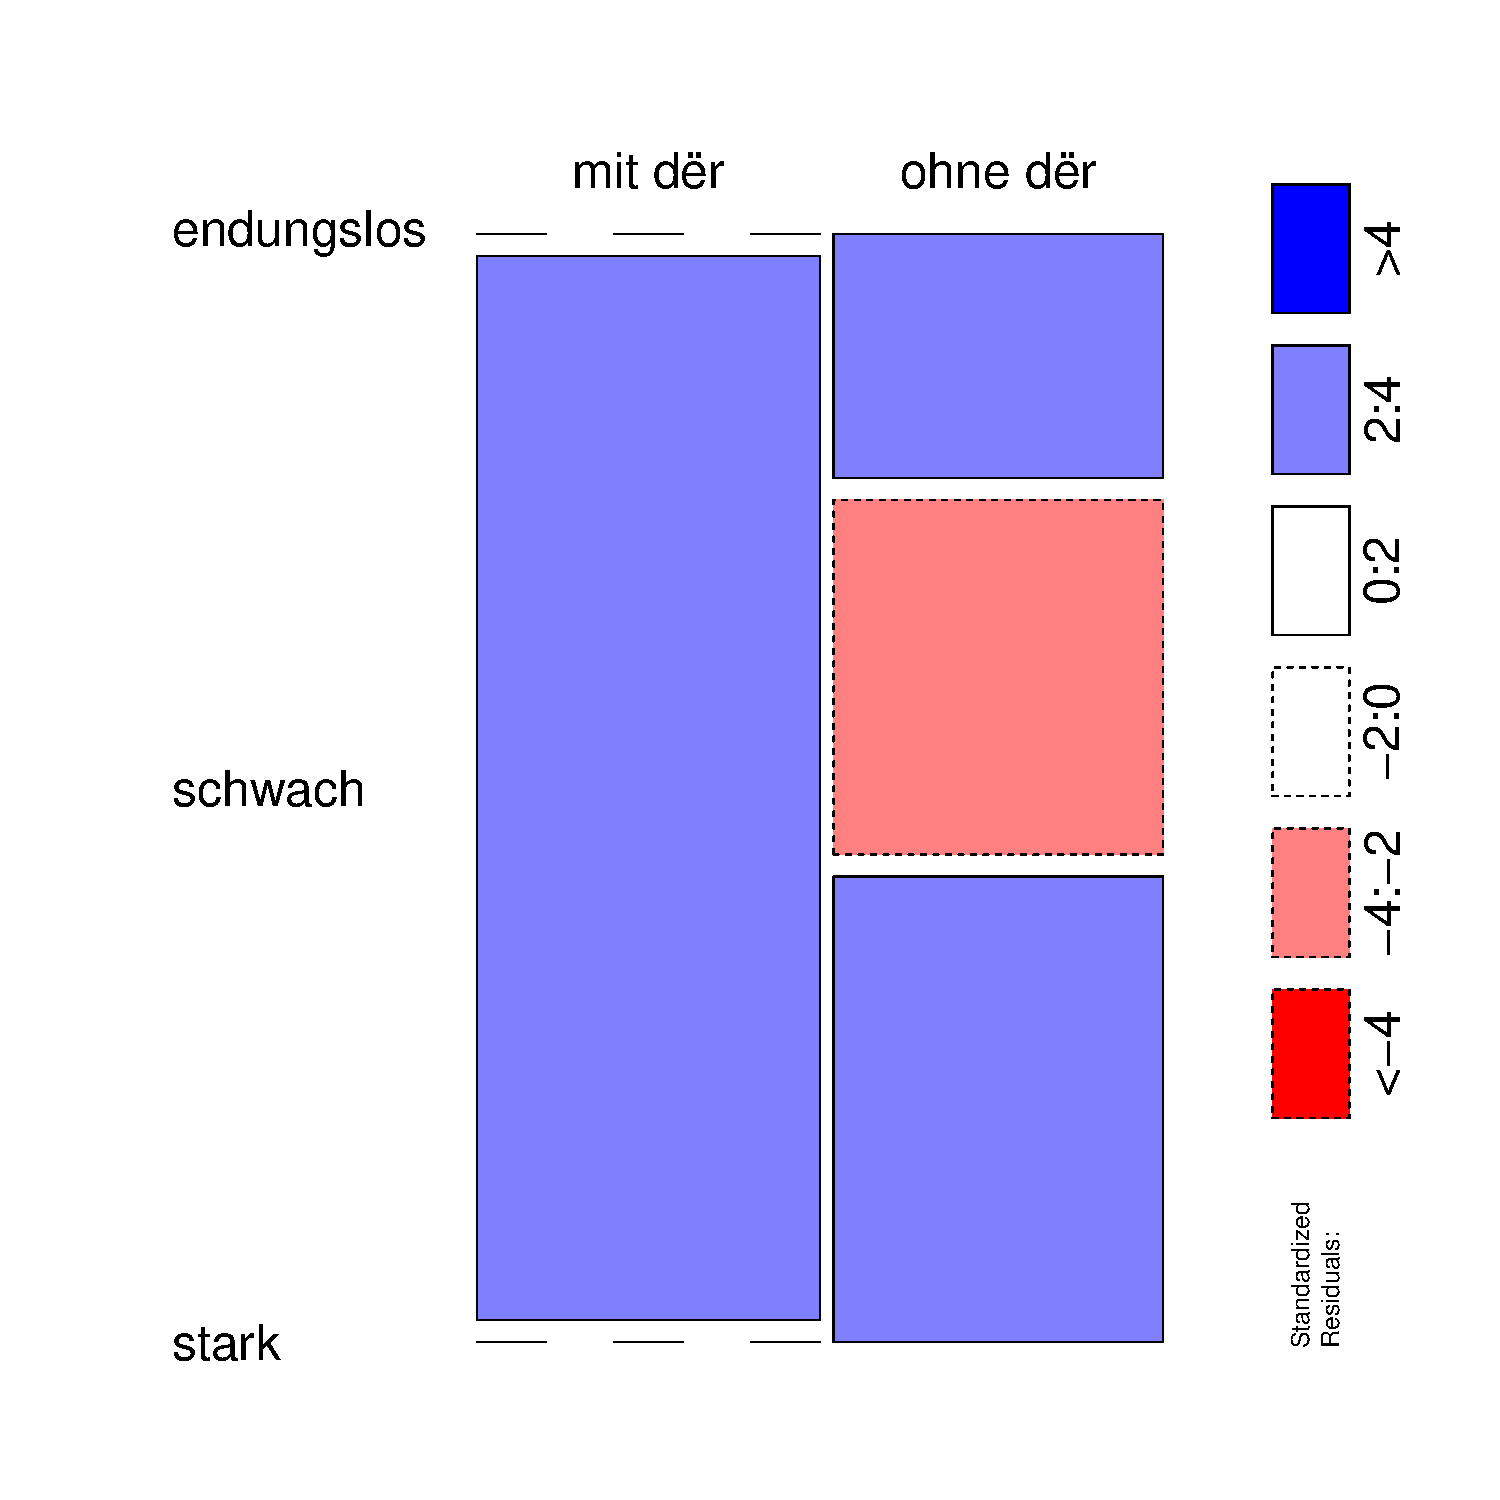
\includegraphics[height=.25\textheight]{generated/images/adjektive-I}
\caption {Isidor}
\end{subfigure}%
\begin{subfigure}[b]{.5\linewidth}
  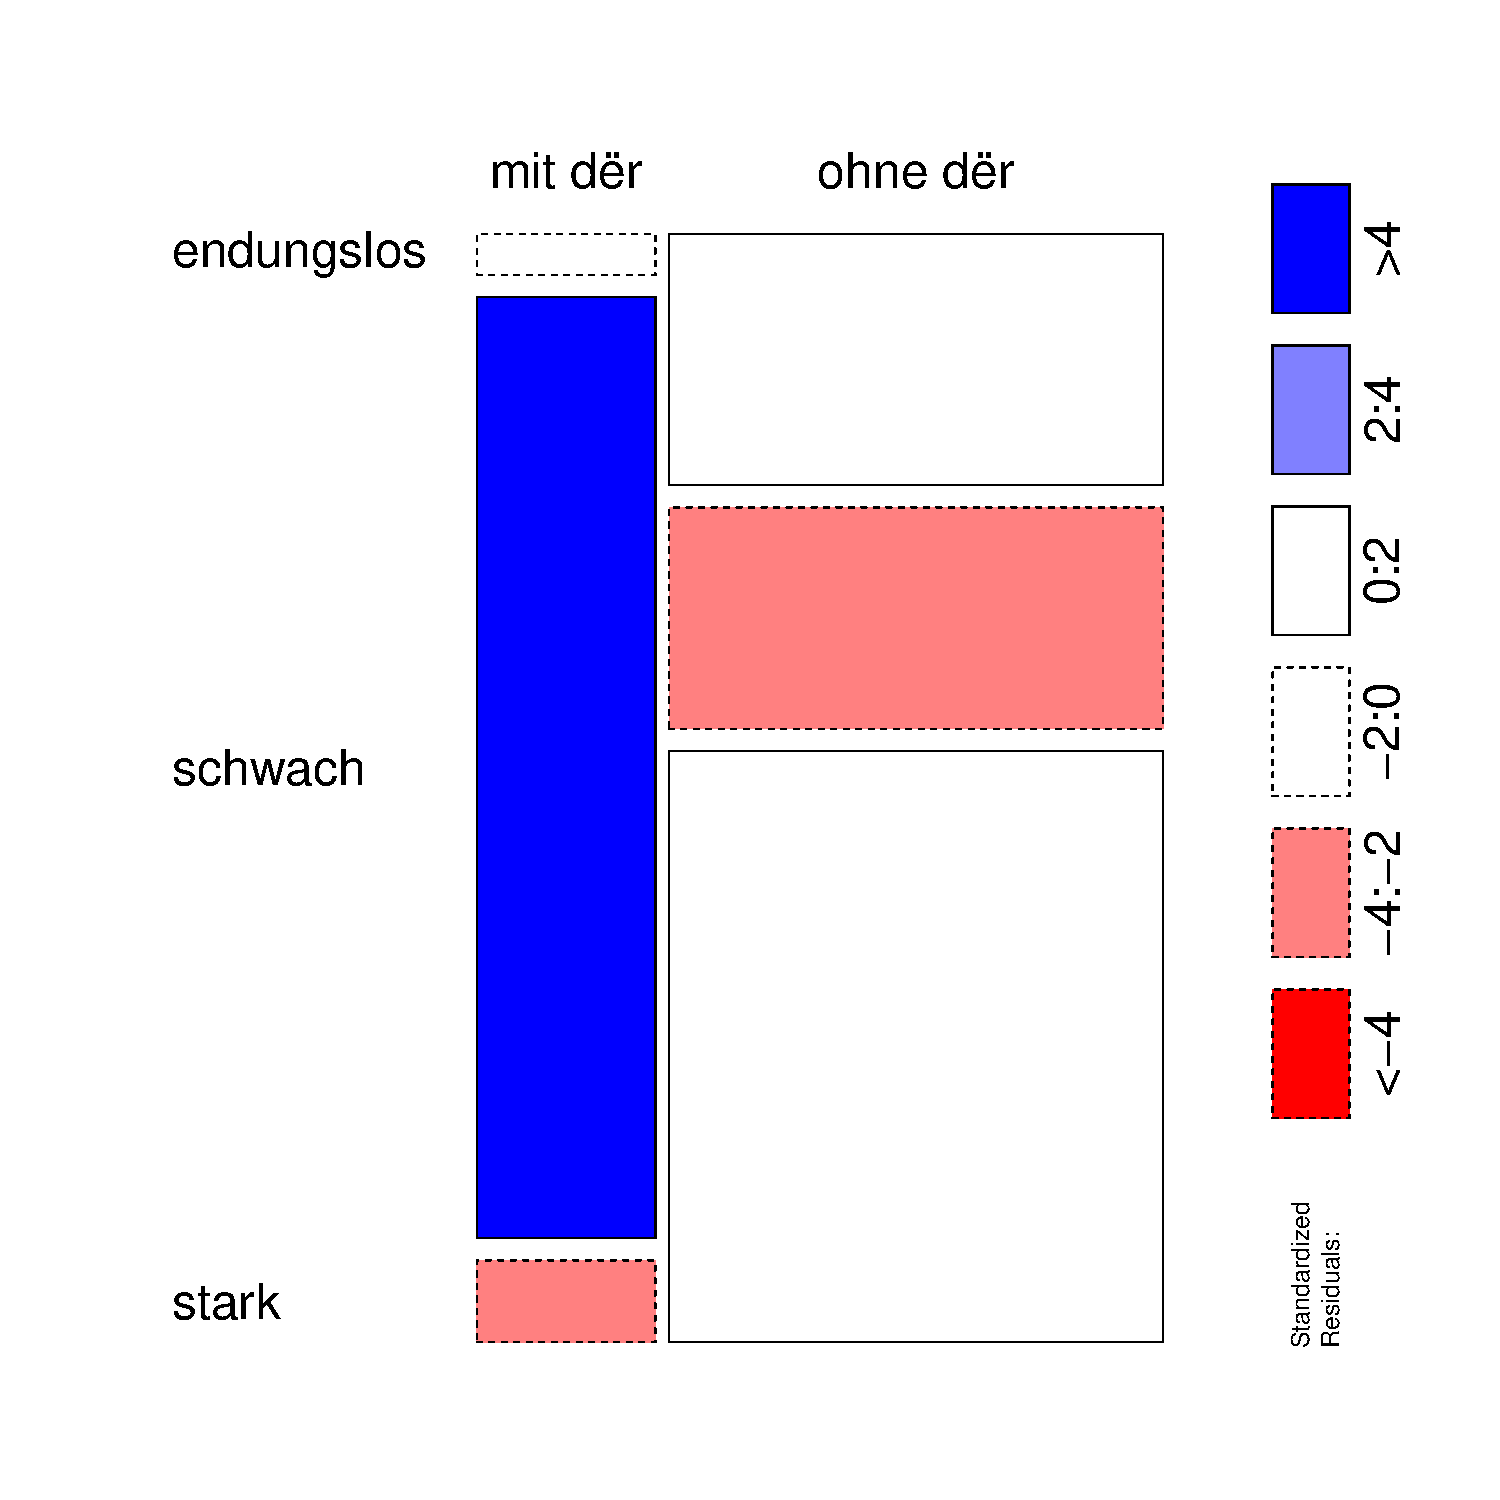
\includegraphics[height=.25\textheight]{generated/images/adjektive-M}
\caption {Monseer Fragmente}
\end{subfigure}

\begin{subfigure}[b]{.5\linewidth}
  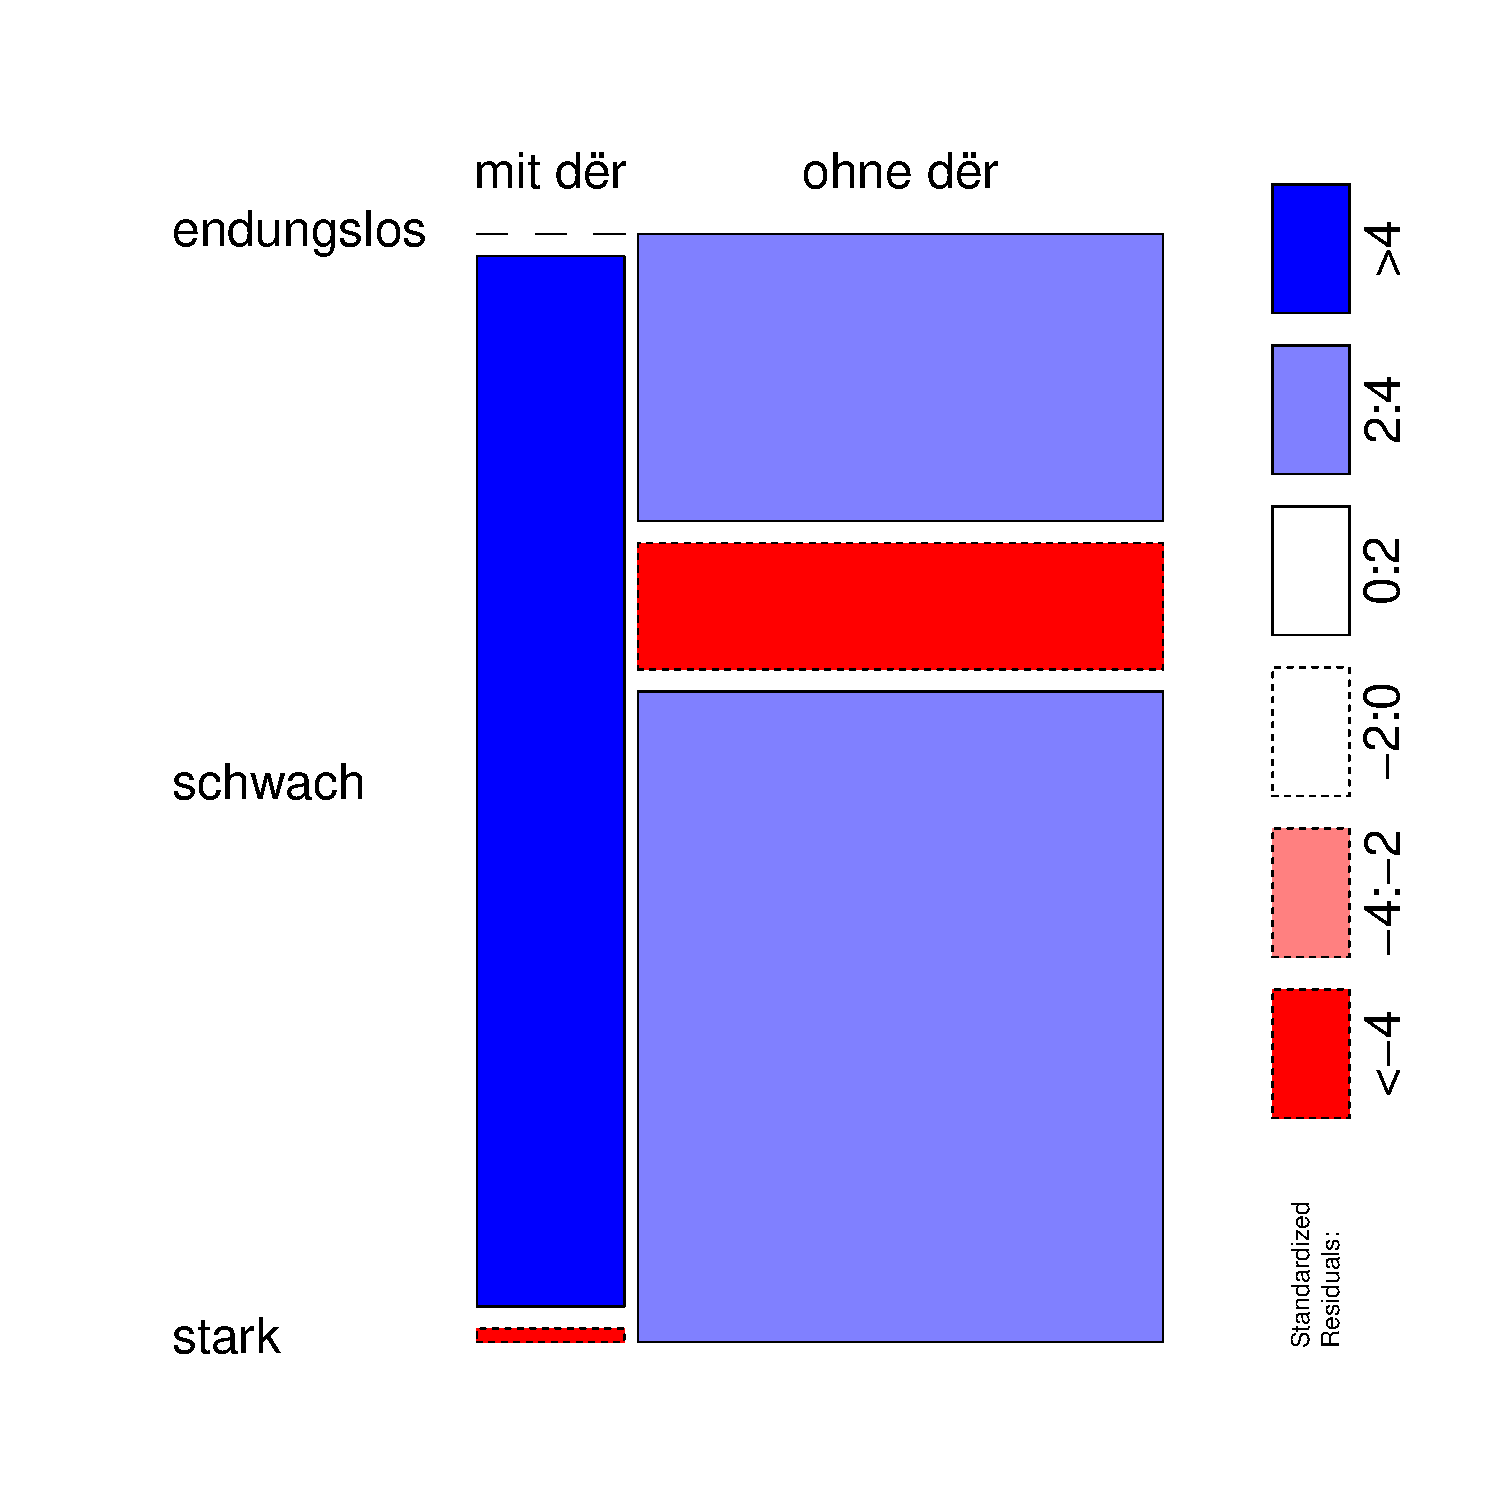
\includegraphics[height=.25\textheight]{generated/images/adjektive-T}
\caption {Tatian}
\end{subfigure}%
\begin{subfigure}[b]{.5\linewidth}
  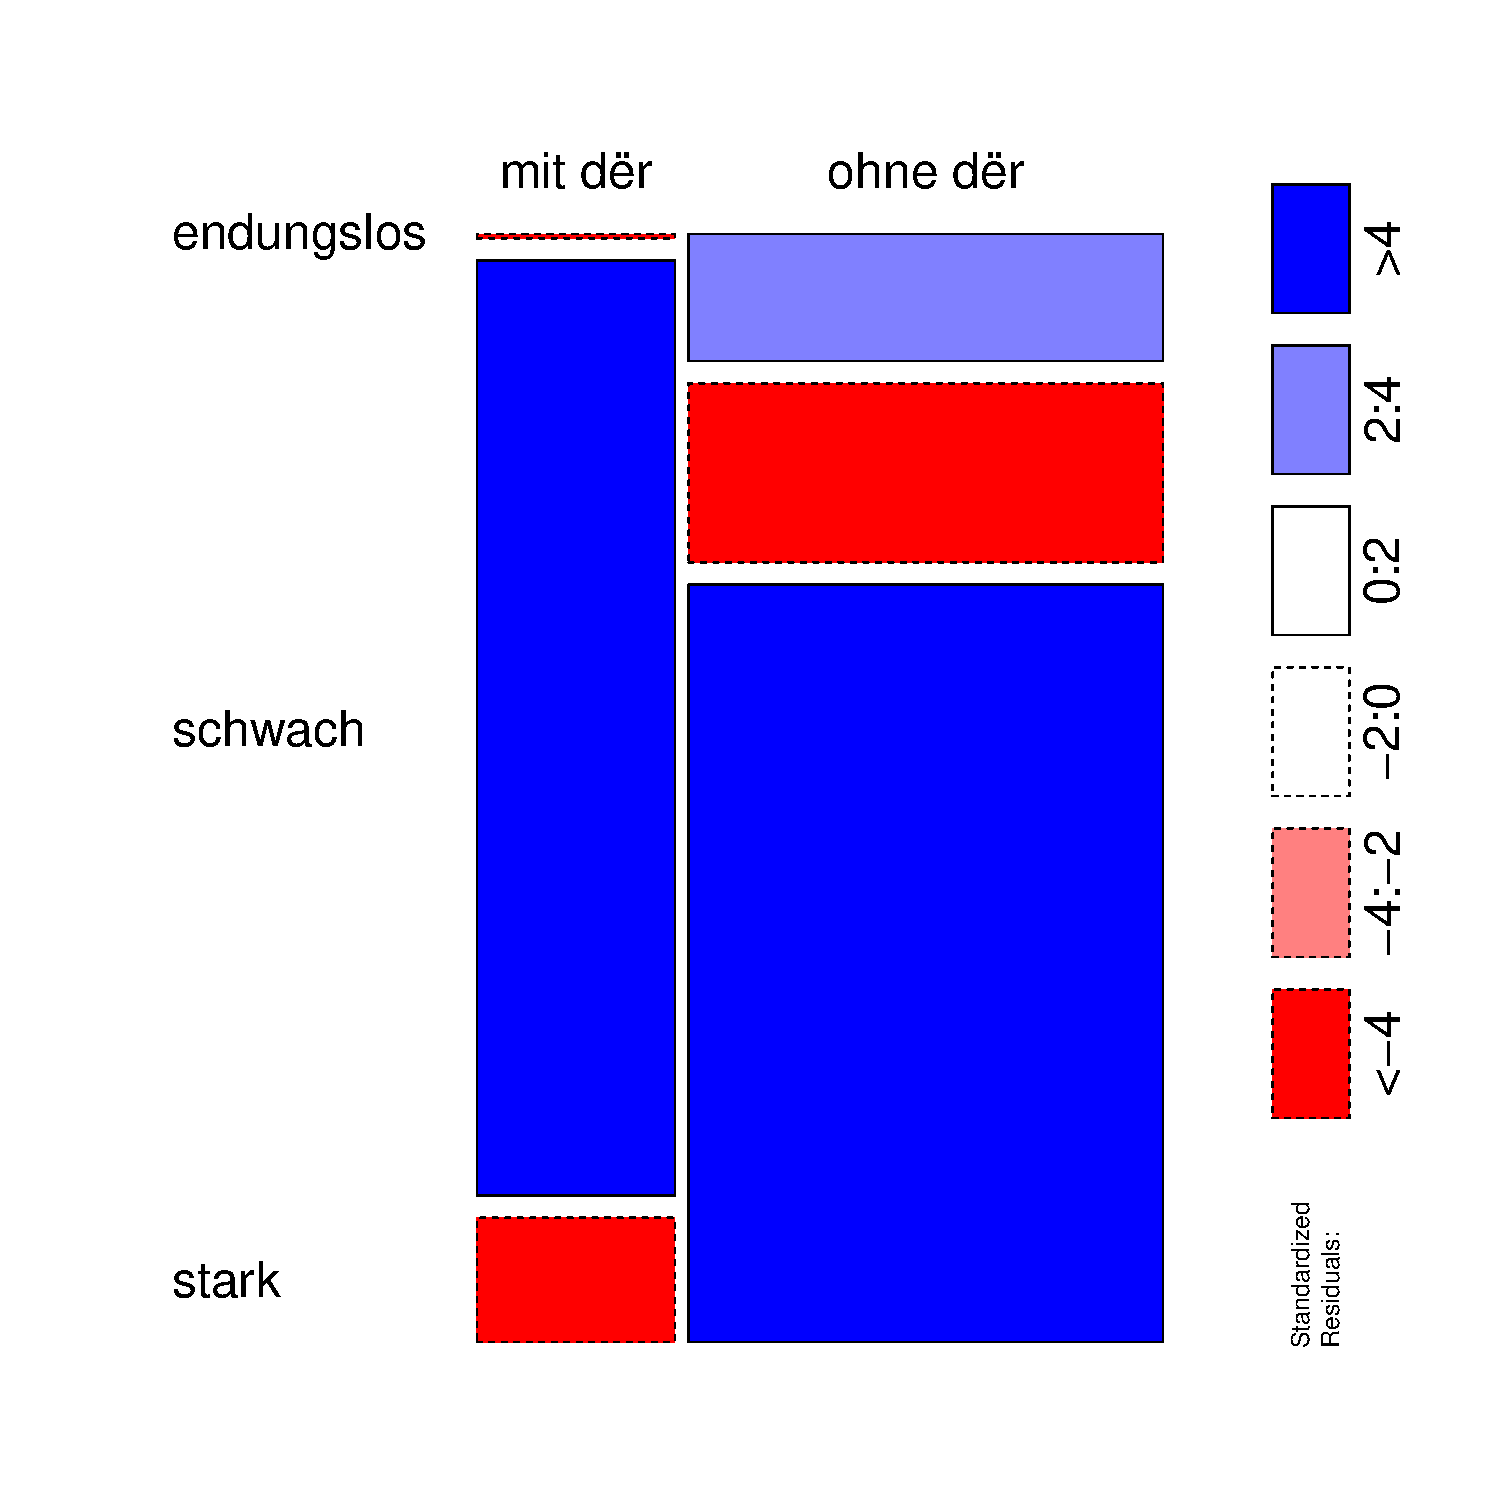
\includegraphics[height=.25\textheight]{generated/images/adjektive-O}
\caption {Otfrid}
\end{subfigure}
\begin{subfigure}[b]{.5\linewidth}
  \includegraphics[height=.25\textheight]{generated/images/adjektive-N}
\caption {Notker}
\end{subfigure}
\caption{\object{dër}-Setzung und Adjektivflexion}
\label{fig:ther-adj}
\end{figure}

\section{Zusammenfassung}

Mit der vorliegenden Korpusuntersuchung \is{Korpus}\is{Korpuslinguistik}wurde eine systematische Analyse von [\object{dër}\,+\,N] im Althochdeutschen vorgenommen. Aus den Daten ist deutlich geworden, dass die Struktur über die Jahrhunderte nicht nur an Frequenz gewinnt, sondern auch in neue Kontexte expandiert. Schon im Isidor, dem ältesten untersuchten Text (um 790), werden mithilfe von \object{dër} häufiger semantisch-definite \is{Semantische Definita} Referenten denotiert als \is{Pragmatische Definita} pragmatisch-definite. Zudem wurden im Isidor auch ein generischer \is{generisch}  Beleg sowie Superlativkonstruktionen \is{Superlativ} mit \object{dër} ausfindig gemacht. Der Anteil der semantisch-definiten \is{Semantische Definita} Kontexte, die mit \object{dër}-Phrasen \is{Phrase} ausgedrückt werden, steigt in den späteren Texten an. Bei Otfrid (um 870) machen sie die Hälfte aller Belege aus und auch Unika \is{Unikum} kommen mit \object{dër} vor. Die \isi{Expansion} ist im jüngsten Text, Notkers Boethius (um 1025), am größten: Hier werden sowohl Phrasen im \isi{Superlativ} als auch Unika \is{Unikum} in der Mehrzahl durch \object{dër}-Phrasen \is{Phrase} ausgedrückt.

Die Auswertungen zur \isi{Belebtheit} zeigen, dass in fast allen Texten menschliche und in den späteren Texten auch konkrete Referenten präferiert mit \object{dër} erscheinen. Abstrakta \is{Abstraktum} und \isi{Massennomen} bleiben hingegen überzufällig häufig undeterminiert. Die Abstrakta \is{Abstraktum} nehmen in den späteren Texten allerdings an Frequenz zu und kommen auch häufiger mit \object{dër} vor. \isi{Massennomen} sind insgesamt nur marginal vertreten. Während  \object{gold} fast immer artikellos erscheint, gibt es vor allem in den jüngeren Texten bei \object{waʒʒar} und \object{bluot} auch Belege mit \object{dër}. Für die Variable \isi{Numerus}, die als Indikator für \isi{Individualität} fungieren sollte, zeigt sich ein gemischtes Bild:  Während im Isidor und im Tatian \object{dër}-Belege häufiger im Singular stehen, sind es im Monseer Matthäus und bei Otfrid Pluralbelege, die eine Präferenz für \object{dër} zeigen. Auch die Untersuchung zur \isi{Relevanz} hat keine eindeutigen Ergebnisse hervorgebracht: Zwar stehen in allen Texten kulturell oder thematisch relevante \is{Relevanz} Referenten an der Spitze der Nomina, die regelmäßig ($\geq$ 80\%) mit \object{dër} determiniert werden. Doch auch denjenigen Nomina, die in der Mehrzahl ohne Artikelwort auftreten, lässt sich eine textuelle oder kulturelle \isi{Relevanz} (darunter \object{sun} oder \object{himil}) nicht absprechen. Im Tatian und bei Notker sind es männliche Referenten, die signifikant häufiger mit \object{dër} determiniert werden, bei Otfrid hingegen weibliche Referenten. Die Stichprobenanalyse zur semantischen Rolle \is{Semantische Rolle} hat gezeigt, dass agentivische Referenten stärker als andere Referenten zur \object{dër}-Setzung tendieren. Aus der globalen Auswertung von Präpositionalphrasen \is{Präpositionalphase (PP)} lässt sich ableiten, dass weniger zentrale Partizipanten länger undeterminiert bleiben. 

Die Analysen zur Struktur der Nominalphrase \is{Nominalsyntax}\is{Nominalphrase (NP)}legen offen, dass der Großteil aller Substantive \is{Substantiv} (Unika \is{Unikum} und Eigennamen \is{Eigenname} ausgeschlossen) pränominal determiniert wird. Während in den frühen Texten zu diesen Determinierern \is{Determinierer} auch adnominale Genitive \is{Genitivattribut} zählen, sind es in den späteren Texten vor allem flektierbare \is{Flexion} Elemente, allen voran \object{dër}. Sie präferieren eindeutig die Voranstellung. Nur Otfrids Evangelienbuch, der einzige poetische Text, zeigt ein freieres Stellungsverhalten, allerdings kommen auch hier die postnominalen \object{dër}-Belege sowie Possessiva \is{Possessivum} und Indefinita \is{Indefinitheit} nicht über einstellige Prozentwerte. Im Gegensatz zu stark flektierten \is{Flexion} und endungslosen Adjektiven \is{Adjektiv} stehen schwach flektierte \is{Flexion} und damit individualisierende Adjektive überzufällig häufig mit \object{dër}.
